%Jorge: ver. barbaria; notas fora
%Jorge: Ajustar quebra e imagens

%\renewcommand\sectionitem{\vspace{-2ex}{\centering\section[Capítulo \textsc{\thesection}\hspace{1ex}]{\thesection}}}

\chapter*{} %O ateneu
\section{I}

\begingroup
\linenumbers

\noindent\textsc{``Vais encontrar} o mundo, disse"-me meu pai, 
à porta do Ateneu. Coragem para a luta.'' 


Bastante experimentei depois a verdade deste aviso, que
me despia, num gesto, das ilusões de criança educada exoticamente na
estufa de carinho que é o regime do amor doméstico; diferente do que se
encontra fora, tão diferente, que parece o poema dos cuidados maternos
um artifício sentimental, com a vantagem única de fazer mais sensível a
criatura à impressão rude do primeiro ensinamento, têmpera brusca da
\wfigura{1}{2.6}{l}
vitalidade na influência de um novo clima rigoroso. Lembramo"-nos,
entretanto, com saudade hipócrita, dos felizes tempos; como se a mesma
incerteza de hoje, sob outro aspecto, não nos houvesse perseguido
outrora, e não viesse de longe a enfiada das decepções que nos ultrajam. 

Eufemismo, os felizes tempos, eufemismo apenas, igual aos
outros que nos alimentam, a saudade dos dias que correram como
melhores. Bem considerando, a atualidade é a mesma em todas as datas.
Feita a compensação dos desejos que variam, das aspirações que se
transformam, alentadas perpetuamente do mesmo ardor, sobre a mesma base
fantástica de esperanças, a atualidade é uma. Sob a coloração cambiante
das horas, um pouco de ouro mais pela manhã, um pouco mais de púrpura
ao crepúsculo --- a paisagem é a mesma de cada lado, beirando a estrada
da vida. 

Eu tinha onze anos. 

Frequentara como externo, durante alguns
meses, uma escola familiar do Caminho Novo, onde algumas senhoras
inglesas, sob a direção do pai, distribuíam educação à infância como
melhor lhes parecia. Entrava às nove horas, timidamente, ignorando as
lições com a maior regularidade, e bocejava até as duas, torcendo"-me
de insipidez sobre os carcomidos bancos que o colégio comprara, de
pinho e usados, lustrosos do contato da malandragem de não sei quantas
gerações de pequenos. Ao meio"-dia, davam"-nos pão com manteiga. Esta
recordação gulosa é o que mais pronunciadamente me ficou dos meses de
externato; com a lembrança de alguns companheiros --- um que gostava de
fazer rir à aula, espécie interessante de mono louro, arrepiado,
vivendo a morder, nas costas da mão esquerda, uma protuberância calosa
que tinha; outro, adamado, elegante, sempre retirado, que vinha à
escola de branco, engomadinho e radioso, fechada a blusa em diagonal do
ombro à cinta por botões de madrepérola. Mais ainda: a primeira vez que
ouvi certa injúria crespa, um palavrão cercado de terror no
estabelecimento, que os partistas denunciavam às mestras por duas
iniciais como em monograma. 

Lecionou"-me depois um professor em domicílio. 

Apesar deste ensaio da vida escolar a que me sujeitou a
família, antes da verdadeira provação, eu estava perfeitamente virgem
para as sensações novas da nova fase. O internato! Destacada do
conchego placentário da dieta caseira, vinha próximo o momento de se
definir a minha individualidade. Amarguei por antecipação o adeus às primeiras alegrias;
olhei triste os meus brinquedos, antigos já! os meus queridos pelotões
de chumbo! espécie de museu militar de todas as fardas, de todas as
bandeiras, escolhida amostra da força dos estados, em proporções de
microscópio, que eu fazia formar a combate como uma ameaça tenebrosa ao
equilíbrio do mundo; que eu fazia guerrear em desordenado aperto, --- 
massa tempestuosa das antipatias geográficas, encontro definitivo e
ebulição dos seculares ódios de fronteira e de raça; que eu pacificava
por fim, com uma facilidade de Providência Divina, intervindo
sabiamente, resolvendo as pendências pela concórdia promíscua das
caixas de pau. Força era deixar à ferrugem do abandono o elegante vapor
da linha circular do lago, no jardim, onde talvez não mais tornasse a
perturbar com a palpitação das rodas a sonolência morosa dos peixinhos,
rubros, dourados, argentados, pensativos à sombra dos tinhorões, na
transparência adamantina da água\ldots{} 

Mas um movimento animou"-me, primeiro estímulo sério da vaidade: 
distanciava"-me da comunhão da família, como um homem! ia por minha conta 
empenhar a luta dos merecimentos; e a confiança nas próprias forças sobrava. 
Quando me disseram que estava a escolha feita da casa de educação que me devia
receber, a notícia veio achar"-me em armas para a conquista audaciosa
do desconhecido. 

Um dia, meu pai tomou"-me pela mão, minha mãe
beijou"-me a testa, molhando"-me de lágrimas os cabelos e eu parti.

Duas vezes fora visitar o Ateneu antes da minha instalação. 

Ateneu era o grande colégio da época. Afamado por um sistema de nutrido reclame,
mantido por um diretor que de tempos a tempos reformava o
estabelecimento, pintando"-o jeitosamente de novidade, como os
negociantes que liquidam para recomeçar com artigos de última remessa,
o Ateneu desde muito tinha consolidado crédito na preferência dos pais;
sem levar em conta a simpatia da meninada, a cercar de aclamações o
bombo vistoso dos anúncios. 

O Dr.\,Aristarco Argolo de Ramos, da
conhecida família do Visconde de Ramos, do Norte, enchia o Império com
o seu renome de pedagogo. Eram boletins de propaganda pelas Províncias,
conferências em diversos pontos da cidade, a pedidos, à sustância,
atochando a imprensa dos lugarejos, caixões, sobretudo, de livros
elementares, fabricados às pressas com o ofegante e esbaforido concurso
de professores prudentemente anônimos, caixões e mais caixões de
volumes cartonados em Leipzig, inundando as escolas públicas de toda a
parte com a sua invasão de capas azuis, róseas, amarelas, em que o nome
de Aristarco, inteiro e sonoro, oferecia"-se ao pasmo venerador dos
esfaimados de alfabeto dos confins da Pátria. Os lugares que os não
procuravam eram um belo dia surpreendidos pela enchente, gratuita,
espontânea, irresistível! E não havia senão aceitar a farinha daquela
marca para o pão do espírito. E engordavam as letras, à força, daquele
pão. Um benemérito. Não admira que em dias de gala, íntima ou nacional,
festas do colégio ou recepções da coroa, o largo peito do grande
educador desaparecesse sob constelações de pedraria, opulentando a
nobreza de todos os honoríficos berloques. 
\wfigura{2}{3.6}{d}

Nas ocasiões de aparato é que se podia tomar o pulso ao homem. 
Não só as condecorações
gritavam"-lhe do peito como uma couraça de grilos: \textit{Ateneu!} \textit{Ateneu!}
Aristarco todo era um anúncio. Os gestos, calmos, soberanos, eram de um
rei --- o autocrata excelso dos silabários; a pausa hierática do andar
deixava sentir o esforço, a cada passo, que ele fazia para levar
adiante, de empurrão, o progresso do ensino público; o olhar
fulgurante, sob a crispação áspera dos supercílios de monstro japonês,
penetrando de luz as almas circunstantes --- era a educação da
inteligência; o queixo, severamente escanhoado, de orelha a orelha,
lembrava a lisura das consciências limpas --- era a educação moral. A
própria estatura, na imobilidade do gesto, na mudez do vulto, a simples
estatura dizia dele: aqui está um grande homem\ldots{} não veem os 
côvados de Golias?!\footnote{ Referência à passagem bíblica em que Davi mata o gigante Golias. 
Côvado é uma antiga medida equivalente a 66 cm. [\versal{N.}~da \versal{E.}]}\ldots{} 
Retorça"-se sobre tudo isto um par de 
bigodes, volutas maciças de fios alvos, torneadas a capricho, cobrindo os lábios, fecho
de prata sobre o silêncio de ouro, que tão belamente impunha como o
retraimento fecundo do seu espírito, --- teremos esboçado, moralmente,
materialmente, o perfil do ilustre diretor. Em suma, um personagem que,
ao primeiro exame, produzia"-nos a impressão de um enfermo, desta
enfermidade atroz e estranha: a obsessão da própria estátua. Como
tardasse a estátua, Aristarco interinamente satisfazia"-se com a
afluência dos estudantes ricos para o seu instituto. De fato, os
educandos do Ateneu significavam a fina flor da mocidade brasileira. 

A irradiação do \textit{réclame}\footnote{ Palavra francesa que designa 
qualquer tipo de publicidade, por meio de folheto, anúncio, cartaz etc. 
[\versal{N.}~da \versal{E.}]} alongava de tal modo os tentáculos através do
país, que não havia família de dinheiro, enriquecida pela setentrional
borracha ou pela charqueada do sul, que não reputasse um compromisso de
honra com a posteridade doméstica mandar dentre seus jovens, um, dois,
três representantes abeberar"-se à fonte espiritual do Ateneu. 

Fiados nesta seleção apuradora, que é comum o erro sensato de julgar melhores
famílias as mais ricas, sucedia que muitos, indiferentes mesmo e
sorrindo do estardalhaço da fama, lá mandavam os filhos. Assim entrei eu. 

A primeira vez que vi o estabelecimento, foi por uma festa de
encerramento de trabalhos. 

Transformara"-se em anfiteatro uma das
grandes salas da frente do edifício, exatamente a que servia de capela;
paredes estucadas de suntuosos relevos, e o teto aprofundado em largo
medalhão, de magistral pintura, onde uma aberta de céu azul despenhava
aos cachos deliciosos anjinhos, ostentando atrevimentos róseos de
carne, agitando os minúsculos pés e as mãozinhas, desatando fitas de
gaze no ar. Desarmado o oratório, construíram"-se bancadas circulares,
que encobriam o luxo das paredes. Os alunos ocupavam a arquibancada.
Como a maior concorrência preferia sempre a exibição dos exercícios
ginásticos, solenizada dias depois do encerramento das aulas, a
acomodação deixada aos circunstantes era pouco espaçosa; e o público,
pais e correspondentes em geral, porém mais numeroso do que se
esperava, tinha que transbordar da sala da festa para a imediata. Desta
ante"-sala, trepado a uma cadeira, eu espiava. Meu pai ministrava"-me
informações. Diante da arquibancada, ostentava"-se uma mesa de grosso
pano verde e borlas de ouro. Lá estava o diretor, o ministro do
Império, a comissão dos prêmios. Eu via e ouvia. Houve uma alocução
comovente de Aristarco; houve discursos de alunos e mestres; houve
cantos, poesias declamadas em diversas línguas. O espetáculo
comunicava"-me certo prazer respeitoso. O diretor, ao lado do
ministro, de acanhado físico, fazia"-o incivilmente desaparecer na
brutalidade de um contraste escandaloso. Em \textit{grande tenue}\footnote{ Expressão 
de origem francesa que significa ``traje de gala'' ou ``traje cerimonial''. [\versal{N.}~da \versal{E.}]} 
dos dias graves, sentava"-se elevado no seu orgulho como em um trono. A bela
farda negra dos alunos, de botões dourados, infundia"-me a
consideração tímida de um militarismo brilhante, aparelhado para as
campanhas da ciência e do bem. A letra dos cantos, em coro dos falsetes
indisciplinados da puberdade, os discursos, visados pelo diretor,
pançudos de sisudez, na boca irreverente da primeira idade, como um
\textit{Cendrillon}\footnote{ Título original do conto de Charles Perrault 
conhecido em português como \textit{A gata borralheira}. [\versal{N.}~da \versal{E.}]} 
malfeito da burguesia conservadora, recitados em monotonia
de realejo e gestos rodantes de manivela, ou exagerados, de voz cava e
caretas de tragédia fora de tempo, eu recebia tudo convictamente, como
o texto da bíblia do dever; e as banalidades profundamente lançadas
como as sábias máximas do ensino redentor. Parecia"-me estar vendo a
legião dos amigos do estudo, mestres à frente, na investida heroica do
obscurantismo, agarrando pelos cabelos, derribando, calcando aos pés a
Ignorância e o Vício, misérrimos trambolhos, consternados e esperneantes. 

Um discurso principalmente impressionou"-me. À direita
da comissão dos prêmios, ficava a tribuna dos oradores. Galgou"-a
firme, tesinho, o Venâncio, professor do colégio, a quarenta mil"-réis
por matéria, mas importante, sabendo falar grosso o timbre de
independência, mestiço de bronze, pequenino e tenaz, que havia de varar
carreira mais tarde. O discurso foi o confronto chapa dos torneios
medievais com o moderno certame das armas da inteligência; depois, uma
preleção pedagógica, tacheada de flores de retórica a martelo; e a
apologia da vida de colégio, seguindo"-se a exaltação do Mestre em
geral e a exaltação, em particular, de Aristarco e do Ateneu. ``O
mestre, perorou Venâncio, é o prolongamento do amor paterno, é o complemento da
ternura das mães, o guia zeloso dos primeiros passos, na senda
escabrosa que vai às conquistas do saber e da moralidade. Experimentado
no labutar cotidiano da sagrada profissão, o seu auxílio ampara"-nos
como a Providência na Terra; escolta"-nos assíduo como um anjo de
guarda; a sua lição prudente esclarece"-nos a jornada inteira do futuro.
Devemos ao pai a existência do corpo; o mestre cria"-nos o espírito
(sorites de sensação), e o espírito é a força que impele, o impulso que
triunfa, o triunfo que nobilita, o enobrecimento que glorifica, e a
glória é o ideal da vida, o louro do guerreiro, o carvalho do artista,
a palma do crente! A família é o amor no lar, o estado é a segurança
civil; o mestre, com o amor forte que ensina e corrige, prepara"-nos
para a segurança íntima inapreciável da vontade. Acima de Aristarco --- 
Deus! Deus tão"-somente; abaixo de Deus --- Aristarco.'' 

Um último gesto espaçoso, como um jamegão no vácuo, arrematou o rapto de
eloquência. 

Eu me sentia compenetrado daquilo tudo; não tanto por
entender bem, como pela facilidade da fé cega a que estava disposto. As
paredes pintadas da ante"-sala imitavam pórfiro verde; em frente ao
pórtico aberto para o jardim, graduava"-se uma ampla escada, caminho
do andar superior. Flanqueando a majestosa porta desta escada, havia
dois quadros de alto"-relevo: à direita uma alegoria das artes e do
estudo, à esquerda as indústrias humanas, meninos nus como nos frisos
de Kaulbach, risonhos, com a ferramenta simbólica --- psicologia pura
do trabalho, modelada idealmente na candura do gesso e da inocência.
Eram meus irmãos! Eu estava a esperar que um deles convidativo me
estendesse a mão para o bailado feliz que os levava. Oh! que não seria
o colégio, tradução concreta da alegoria, ronda angélica de corações à
porta de um templo, dulia permanente das almas jovens no ritual austero
da virtude! 

Por ocasião da festa da ginástica, voltei ao colégio. 

O Ateneu estava situado no Rio Comprido, extremo, ao chegar aos morros.

As eminências de sombria pedra e a vegetação selvática debruçavam sobre
o edifício um crepúsculo de melancolia, resistente ao próprio sol a
pino dos meios"-dias de novembro. Esta melancolia era um plágio ao
detestável pavor monacal de outra casa de educação, o negro Caraça de
Minas. Aristarco dava"-se palmas desta tristeza aérea --- a atmosfera
moral da meditação e do estudo, definia, escolhida a dedo para maior
luxo da casa, como um apêndice mínimo da arquitetura. 

No dia da \textit{festa da educação física}, como rezava o programa (programa de arromba, 
porque o secretário do diretor tinha o talento dos programas), não percebi a
sensação de ermo tão acentuada em sítios montanhosos, que havia de
notar depois. As galas do momento faziam sorrir a paisagem. O arvoredo
do imenso jardim, entretecido a cores por mil bandeiras, brilhava ao
sol vivo com o esplendor de estranha alegria; os vistosos panos, em
meio da ramagem, fingiam flores colossais, numa caricatura extravagante
de primavera; os galhos frutificavam em lanternas venezianas, pomos de
papel enormes, de uma uberdade carnavalesca. Eu ia carregado, no
impulso da multidão. Meu pai prendia"-me solidamente o pulso, que me
não extraviasse. 

Mergulhado na onda, eu tinha que olhar para cima, para
respirar. Adiante de mim, um sujeito mais próximo fez"-me rir; levava
de fora a fralda da camisa\ldots{} Mas não era fralda; verifiquei que era o
lenço. Do chão subia um cheiro forte de canela pisada; através das
árvores, com intervalos, passavam rajadas de música, como uma
tempestade de filarmônicas. 

Um último aperto mais rijo estalando"-me as costelas espremeu"-me 
por um estreito corte num muro, para o espaço livre. 

Em frente, um gramal vastíssimo. Rodeava"-o uma ala de
galhardetes, contentes no espaço, com o pitoresco dos tons enérgicos
cantando vivo sobre a harmoniosa surdina do verde das montanhas. Por
todos os lados apinhava"-se o povo. Voltando"-me, divisei, ao longo
do muro, duas linhas de estrado com cadeiras quase exclusivamente
ocupadas por senhoras, fulgindo os vestuários, em violenta confusão de
colorido. Algumas protegiam o olhar com a mão enluvada, com o leque, à
altura da fronte, contra a rutilação do dia num bloco de nuvens que crescia do
céu. Acima do estrado, balouçavam docemente e sussurravam bosquetes de
bambu, projetando franjas longuíssimas de sombra pelo campo de relva.

Algumas damas empunhavam binóculos. Na direção dos binóculos
distinguia"-se um movimento alvejante. Eram os rapazes. ``Aí vêm!
disse"-me meu pai; vão desfilar por diante da princesa.'' A princesa
imperial, regente nessa época, achava"-se à direita em gracioso
palanque de sarrafos. 

Momentos depois adiantavam"-se por mim os alunos
do Ateneu. Cerca de trezentos; produziam"-me a impressão do
inumerável. Todos de branco, apertados em larga cinta vermelha, com
alças de ferro sobre os quadris e na cabeça um pequeno gorro cingido
por um cadarço de pontas livres. Ao ombro esquerdo traziam laços
distintivos das turmas. Passaram a toque de clarim, sopesando os
petrechos diversos dos exercícios. Primeira turma, os \textit{halteres},
segunda, as \textit{maças}, terceira, as \textit{barras}. 

Fechavam a marcha, desarmados,
os que figurariam simplesmente nos exercícios gerais. 

Depois de longa volta, a quatro de fundo, dispuseram"-se em pelotões, invadiram o
gramal, e, cadenciados pelo ritmo da banda de colegas, que os esperava
no meio do campo, com a certeza de amestrada disciplina, produziram as
manobras perfeitas de um exército sob o comando do mais raro instrutor.

Diante das fileiras, Bataillard, o professor de ginástica, exultava,
envergando a altivez do seu sucesso na extremada elegância do talhe,
multiplicando por milagroso desdobramento o compêndio inteiro da
capacidade profissional, exibida em galeria por uma série infinita de
atitudes. A admiração hesitava a decidir"-se pela formosura masculina
e rija da plástica de músculos a estalar o brim do uniforme, que ele
trajava branco como os alunos, ou pela nervosa celeridade dos
movimentos, efeito elétrico de lanterna mágica, respeitando"-se na
variedade prodigiosa a unidade da correção suprema. 

Ao peito tilintavam"-lhe as agulhetas do comando, apenas de cordões vermelhos
em trança. Ele dava as ordens fortemente, com uma vibração penetrante
de corneta que dominava à distância, e sorria à docilidade mecânica dos
rapazes. Como oficiais subalternos, auxiliavam"-no os chefes de turma;
postados devidamente com os pelotões, sacudindo à manga distintivos de
fita verde e canutilho. 

Acabadas as evoluções, apresentaram"-se os
exercícios. Músculos do braço, músculos do tronco, tendões dos
jarretes, a teoria toda do \textit{corpore sano}\footnote{ Da frase latina 
\textit{mens sana in corpore sano}, do poeta romano Juvenal: 
``mente sã em um corpo são''. [\versal{N.}~da \versal{E.}]} foi praticada valentemente ali,
precisamente, com a simultaneidade exata das extensas máquinas. Houve
após, o assalto aos aparelhos. Os aparelhos alinhavam"-se a uma banda
do campo, a começar do palanque da regente. Não posso dar ideia do
deslumbramento que me ficou desta parte. Uma desordem de contorções,
deslocadas e atrevidas; uma vertigem de volteios à barra fixa,
temeridades acrobáticas ao trapézio, às perchas, às cordas, às escadas;
pirâmides humanas sobre as paralelas, deformando"-se para os lados em
curvas de braços e ostentações vigorosas de tórax; formas de estatuária
viva, trêmulas de esforço, deixando adivinhar de longe o estalido dos
ossos desarticulados; posturas de transfiguração sobre invisível apoio;
aqui e ali uma cabecinha loura, cabelos em desordem cacheados à testa,
um rosto injetado pela inversão do corpo, lábios entreabertos ofegando,
olhos semicerrados para escapar à areia dos sapatos, costas de suor,
colando a blusa em pasta, gorros sem dono que caíam do alto e juncavam
a terra; movimento, entusiasmo por toda a parte e a soalheira, branca
nos uniformes, queimando os últimos fogos da glória diurna sobre aquele
triunfo espetaculoso da saúde, da força, da mocidade. 

O professor Bataillard, enrubescido de agitação, rouco de comandar, chorava de
prazer. Abraçava os rapazes indistintamente. Duas bandas militares
revezavam"-se ativamente, comunicando a animação à massa dos
espectadores. O coração pulava"-me no peito com um alvoroço novo, que
me arrastava para o meio dos alunos, numa leva ardente de fraternidade.
Eu batia palmas; gritos escapavam"-me, de que me arrependia quando
alguém me olhava. 

Deram fim à festa os saltos, os páreos de carreira,
as lutas romanas e a distribuição dos prêmios de ginástica, que a mão
egrégia da Sereníssima Princesa e a pouco menos do Esposo Augusto
alfinetavam sobre os peitos vencedores. Foi de ver"-se: os jovens
atletas aos pares aferrados, empuxando"-se, constringindo"-se,
rodopiando, rolando na selva com gritos satisfeitos e arquejos de
arrancada; os corredores, alguns em rigor, respiração medida, beiços
unidos, punhos cerrados contra o corpo, passo miúdo e vertiginoso;
outros irregulares, bracejantes, prodigalizando pernadas, rasgando o ar
a pontapés, numa precipitação desengonçada de avestruz, chegando
esbofados, com placas de poeira na cara, ao poste da vitória. 

Aristarco arrebentava de júbilo. Pusera de parte o comedimento soberano que eu
lhe admirara na primeira festa. De ponto em branco, como a rapaziada, e
chapéu"-do"-chile, distribuía"-se numa ubiquidade impossível de meio
ambiente. Viam"-no ao mesmo tempo a festejar os príncipes com o
risinho nasal, cabritante, entre lisonjeiro e irônico, desfeito em
etiquetas de reverente súdito e cortesão; viam"-no bradando ao
professor de ginástica, a gesticular com o chapéu seguro pela copa;
viam"-no formidável, com o perfil leonino rugir sobre um discípulo que
fugira aos trabalhos, sobre outro que tinha limo nos joelhos de haver
lutado em lugar úmido, gastando tal veemência no ralho, que chegava a
ser carinhoso. 

O figurino campestre rejuvenescera"-o. Sentia as pernas
leves e percorria celerípede a frente dos estrados, cheio de
cumprimentos para os convidados especiais e de interjetivos amáveis
para todos. Perpassava como uma visão de brim claro, súbito extinta
para reaparecer mais viva noutro ponto. Aquela expansão vencia"-nos;
ele irradiava de si, sobre os alunos, sobre os espectadores, o
magnetismo dominador dos estandartes de batalha. Roubava"-nos dois
terços da atenção que os exercícios pediam; indenizava"-nos com o
equivalente em surpresas de vivacidade, que desprendia de si,
profusamente, por erupções de jorro em roda, por ascensões cobrejantes
de girândola, que iam às nuvens, que baixavam depois serenamente,
diluídas na viração da tarde, que os pulmões bebiam. Ator profundo,
realizava ao pé da letra, a valer, o papel diáfano, sutil, metafísico,
de alma da festa e alma do seu instituto. 

Uma coisa o entristeceu, um pequenino escândalo. Seu filho Jorge, 
na distribuição dos prêmios, recusara"-se a beijar a mão da princesa, 
como faziam todos ao receber a medalha. Era republicano o pirralho! 
Tinha já aos quinze anos as
convicções ossificadas na espinha inflexível do caráter! Ninguém
mostrou perceber a bravura. Aristarco, porém, chamou o menino à parte.
Encarou"-o silenciosamente e --- nada mais. E ninguém mais viu o
republicano! Consumira"-se naturalmente o infeliz, cremado ao fogo
daquele olhar! Nesse momento as bandas tocavam o hino da monarquia
jurada, última verba do programa. 

Começava a anoitecer, quando o
colégio formou ao toque de recolher. Desfilaram aclamados, entre alas
de povo, e se foram do campo, cantando alegremente uma canção escolar.

À noite houve baile nos três salões inferiores do lance principal do
edifício e iluminação no jardim. 

\begin{center}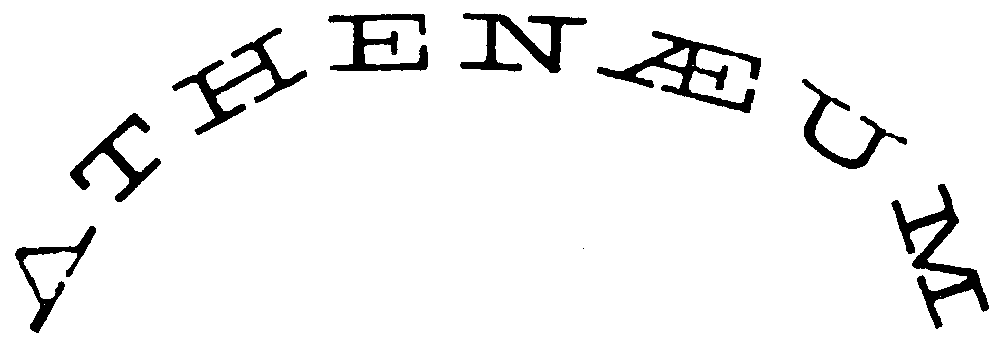
\includegraphics[width=4cm]{3.png}\end{center}

Na ocasião em que me ia embora,
estavam acendendo luzes variadas de Bengala diante da casa. O Ateneu,
quarenta janelas, resplendentes do gás interior, dava"-se ares de
encantamento com a iluminação de fora. Erigia"-se na escuridão da
noite, como imensa muralha de coral flamante, como um cenário animado
de safira com horripilações errantes de sombra, como um castelo
fantasma batido de luar verde emprestado à selva intensa dos romances
cavalheirescos, despertado um momento da legenda morta para uma
entrevista de espectros e recordações. Um jato de luz elétrica,
derivado de foco invisível, feria a inscrição
dourada sobre as janelas centrais no alto do prédio. A uma delas, à sacada,
Aristarco mostrava"-se. Na expressão olímpica do semblante transpirava
a beatitude de um gozo superior. Gozava a sensação prévia, no banho
luminoso, da imortalidade a que se julgava consagrado. Devia ser assim:
--- luz benigna e fria, sobre bustos eternos, o ambiente glorioso do Panteão. A
contemplação da posteridade embaixo. 

Aristarco tinha momentos destes,
sinceros. O anúncio confundia"-se com ele, suprimia"-o, substituía"-o,
e ele gozava como um cartaz que experimentasse o entusiasmo de ser
vermelho. Naquele momento, não era simplesmente a alma do seu
instituto, era a própria feição palpável, a síntese grosseira do
título, o rosto, a testada, o prestígio material do seu colégio,
idêntico com as letras que luziam em auréola sobre a cabeça. As letras,
de ouro, ele, imortal: única diferença. 

\figura{4}{6}

Guardei, na imaginação
infantil, a gravura desta apoteose com o atordoamento ofuscado, mais ou
menos de um sujeito partindo à meia"-noite de qualquer teatro, onde,
em mágica beata, Deus Padre pessoalmente se houvesse prestado a
concorrer para a grandeza do último quadro. Conheci"-o solene na
primeira festa, jovial na segunda; conheci"-o mais tarde em mil
situações, de mil modos; mas o retrato que me ficou para sempre do meu
grande diretor, foi aquele --- o belo bigode branco, o queixo barbeado,
o olhar perdido nas trevas, fotografia estática, na ventura de um raio
elétrico. 

É fácil conceber a atração que me chamava para aquele mundo
tão altamente interessante, no conceito das minhas impressões. Avaliem
o prazer que tive, quando me disse meu pai que eu ia ser apresentado ao
diretor do Ateneu e à matrícula. O movimento não era mais a vaidade,
antes o legítimo instinto da responsabilidade altiva, era uma
consequência apaixonada da sedução do espetáculo, o arroubo de
solidariedade que me parecia prender à comunhão fraternal da escola.
Honrado engano, esse ardor franco por uma empresa ideal de energia e de
dedicação premeditada confusamente, no cálculo pobre de uma experiência
de dez anos. 

O diretor recebeu"-nos em sua residência, com
manifestações ultra de afeto. Fez"-se cativante, paternal; abriu"-nos
amostras dos melhores padrões do seu espírito, evidenciou as faturas do
seu coração. O gênero era bom, sem dúvida nenhuma; que apesar do paletó
de seda e do calçado raso com que se nos apresentava, apesar da bondosa
familiaridade com que declinava até nós, nem um segundo o destituí da
altitude de divinização em que o meu critério embasbacado o aceitara.

Verdade é que não era fácil reconhecer ali, tangível e em carne, uma
entidade outrora da mitologia das minhas primeiras concepções
antropomórficas; logo após Nosso Senhor, o qual eu imaginara velho,
feíssimo, barbudo, impertinente, corcunda, ralhando por trovões,
carbonizando meninos com o corisco. Eu aprendera a ler pelos livros
elementares de Aristarco, e o supunha velho como o primeiro, porém
rapado, de cara chupada, pedagógica, óculos apocalípticos, carapuça
negra de borla, fanhoso, onipotente e mau, com uma das mãos para trás
escondendo a palmatória e doutrinando à humanidade o be"-á"-bá. 

As impressões recentes derrogavam o meu Aristarco; mas a hipérbole
essencial do primitivo transmitia"-se ao sucessor por um mistério de
hereditariedade renitente. Dava"-me gosto então a peleja renhida das
duas imagens e aquela complicação imediata do paletó de seda e do
sapato raso, fazendo aliança com Aristarco \textsc{ii} contra Aristarco \textsc{i}, no
reino da fantasia. Nisto afagaram"-me a cabeça. Era Ele! Estremeci.

``Como se chama o amiguinho?'', perguntou"-me o diretor. 

--- Sérgio\ldots{} dei o nome todo, baixando os olhos e sem esquecer o ``seu criado'' da
estrita cortesia. 

--- Pois, meu caro Sr.\,Sérgio, o amigo há de ter a
bondade de ir ao cabeleireiro deitar fora estes cachinhos\ldots{} 

Eu tinha ainda os cabelos compridos, por um capricho amoroso de minha mãe. O
conselho era visivelmente salgado de censura. O diretor, explicando a
meu pai, acrescentou com o risinho nasal que sabia fazer: ``Sim, senhor,
os meninos bonitos não provam bem no meu colégio\ldots{}'' 

--- Peço licença para defender os meninos bonitos\ldots{} objetou alguém entrando.

Surpreendendo"-nos com esta frase, untuosamente escoada por um
sorriso, chegou a senhora do diretor, D.\,Ema. Bela mulher em plena
prosperidade dos \textit{trinta anos de Balzac},\footnote{ Alusão ao romance de Honoré de Balzac, 
\textit{A mulher de 30 anos}. [\versal{N.}~da \versal{E.}]} 
formas alongadas por graciosa magreza, erigindo porém o tronco sobre
quadris amplos, fortes como a maternidade; olhos negros, pupilas
retintas de uma cor só, que pareciam encher o talho folgado das
pálpebras; de um moreno rosa que algumas formosuras possuem, e que
seria também a cor do jambo, se jambo fosse rigorosamente o fruto
proibido. Adiantava"-se por movimentos oscilados, cadência de minueto
harmonioso e mole que o corpo alternava. Vestia cetim preto justo sobre
as formas, reluzente como pano molhado; e o cetim vivia com ousada
transparência a vida oculta da carne. Esta aparição maravilhou"-me.
Houve as apresentações de cerimônia, e a senhora com um nadinha de
excessivo desembaraço sentou"-se ao divã perto de mim. 

--- Quantos anos tem?, perguntou"-me. 

--- Onze anos\ldots{} 

--- Parece ter seis, com estes lindos cabelos. 

Eu não era realmente desenvolvido. A senhora
colhia"-me o cabelo nos dedos: 

--- Corte e ofereça a mamãe, aconselhou
com uma carícia; é a infância que aí fica, nos cabelos louros\ldots{}
Depois, os filhos nada mais têm para as mães. 

O poemeto de amor materno deliciou"-me como uma divina música. Olhei furtivamente 
para a senhora. Ela conservava sobre mim as grandes pupilas negras, lúcidas,
numa expressão de infinda bondade! Que boa mãe para os meninos, pensava
eu. Depois, voltada para meu pai, formulou sentidamente observações a
respeito da solidão das crianças no internato. 

--- Mas o Sérgio é dos fortes, disse Aristarco, apoderando"-se da palavra. 
Demais, o meu colégio é apenas maior que o lar doméstico. O amor não é precisamente o
mesmo, mas os cuidados de vigilância são mais ativos. São as crianças
os meus prediletos. Os meus esforços mais desvelados são para os
pequenos. Se adoecem e a família está fora, não os confio a um
correspondente\ldots{} Trato"-os aqui, em minha casa. Minha senhora é a
enfermeira. Queria que o vissem os detratores\ldots{} 

Enveredando pelo tema
querido do elogio próprio e do Ateneu, ninguém mais pôde falar\ldots{}

Aristarco, sentado, de pé, cruzando terríveis passadas,
imobilizando"-se a repentes inesperados, gesticulando como um tribuno
de \textit{meetings},\footnote{ Palavra inglesa que significa 
``comícios, reuniões''. [\versal{N.}~da \versal{E.}]} clamando 
como para um auditório de dez mil pessoas,
majestoso sempre, alçando os padrões admiráveis, como um leiloeiro, e
as opulentas faturas, desenrolou, com a memória de uma última
conferência, a narrativa dos seus serviços à causa santa da instrução.
Trinta anos de tentativas e resultados, esclarecendo como um farol
diversas gerações agora influentes no destino do país! E as reformas
futuras? Não bastava a abolição dos castigos corporais, o que já dava
uma benemerência passável. Era preciso a introdução de métodos novos,
supressão absoluta dos vexames de punição, modalidades aperfeiçoadas no
sistema das recompensas, ajeitação dos trabalhos, de maneira que seja a
escola um paraíso, adoção de normas desconhecidas cuja eficácia ele
pressentia, perspicaz como as águias. Ele havia de criar\ldots{} um horror,
a transformação moral da sociedade! 

Uma hora trovejou"-lhe à boca, em
sanguínea eloquência, o gênio do anúncio. Miramo"-lo na inteira
expansão oral, como, por ocasião das festas, na plenitude da sua
vivacidade prática. Contemplávamos (eu com aterrado espanto) distendido
em grandeza épica --- \textit{o homem"-sanduíche} da educação nacional. Lardeado
entre dois monstruosos cartazes. Às costas, o seu passado incalculável
de trabalhos; sobre o ventre, para a frente, o seu futuro: a \textit{réclame}
dos imortais projetos.


\section{II}

\noindent\textsc{Abriam"-se as aulas} a 15 de fevereiro. 

De manhã, à hora regulamentar, compareci. 
O diretor, no escritório do estabelecimento, ocupava uma
cadeira rotativa junto à mesa de trabalho. Sobre a mesa um grande livro
abria"-se em colunas maciças de escrituração e linhas encarnadas.

Aristarco, que consagrava as manhãs ao governo financeiro do colégio,
conferia, analisava os assentamentos do guarda"-livros. De momento a
momento entravam alunos. Alguns acompanhados. A cada entrada, o diretor
lentamente fechava o livro comercial, marcando a página com um alfanje
de marfim; fazia girar a cadeira e soltava interjeições de acolhimento,
oferecendo episcopalmente a mão peluda ao beijo contrito e filial dos meninos. 

Os maiores, em regra, recusavam"-se à cerimônia e partiam com
um simples aperto de mão. 

O rapaz desaparecia, levando o sorriso pálido
na face, saudoso da vadiação ditosa das férias. O pai, o
correspondente, o portador, despedia"-se, depois de banais
cumprimentos, ou palavras a respeito do estudante, amenizadas pela
gracinha da bonomia superior de Aristarco, que punha habilmente um
sujeito fora de portas com o riso fanhoso e o simples modo impelido de
segurar"-lhe os dedos. 

\figura{5}{6}

A cadeira girava de novo à posição primitiva; o
livro da escrituração espalmava outra vez as páginas enormes; e a
figura paternal do educador desmanchava"-se, volvendo a
simplificar"-se na esperteza atenta e seca do gerente. 

A este vaivém de atitudes, feição dupla de uma mesma individualidade e contingência
comum dos sacerdócios, estava tão habituado o nosso diretor, que nenhum
esforço lhe custava a manobra. O especulador e o levita ficavam"-lhe
dentro em camaradagem íntima, \textit{bras dessus, bras dessous}.\footnote{ Expressão idiomática 
francesa que significa ``de braços dados''. [\versal{N.}~da \versal{E.}]}
Sabiam, sem prejuízo da oportunidade, aparecer por alternativa ou simultaneamente;
eram como duas almas inconhas num só corpo. 

Soldavam"-se nele o educador e o empresário com uma perfeição rigorosa de acordo, 
dois lados da mesma medalha; opostos, mas justapostos. 

Quando meu pai entrou
comigo havia no semblante de Aristarco uma pontinha de aborrecimento.
Decepção talvez de estatística, o número dos estudantes novos não
compensando o número dos perdidos, as novas entradas não
contrabalançando as despesas do fim do ano\ldots{} Mas a sombra de despeito
apagou"-se logo, como o resto de túnica que apenas tarda a sumir"-se
numa mutação à vista; e foi com uma explosão de contentamento que o
diretor nos acolheu. 

Sua diplomacia dividia"-se por escaninhos
numerados, segundo a categoria de recepção que queria dispensar. Ele
tinha maneiras de todos os graus, segundo a condição social da pessoa.
As simpatias verdadeiras eram raras. No âmago de cada sorriso
morava"-lhe um segredo de frieza que se percebia bem. E duramente se
marcavam distinções políticas, distinções financeiras, distinções
baseadas na crônica escolar do discípulo, baseadas na razão discreta
das notas do guarda"-livros. Às vezes, uma criança sentia a alfinetada
no jeito da mão a beijar. Saía indagando consigo o motivo daquilo, que
não achava em suas contas escolares\ldots{} O pai estava dois trimestres
atrasado. 

Por diversas causas a minha recepção devia ser das melhores.
Efetivamente; Aristarco levantou"-se ao nosso encontro e nos conduziu
à sala especial das visitas. 

Saiu depois a mostrar o estabelecimento,
as coleções em armários dos objetos próprios para facilitar o ensino.
Eu via tudo curiosamente, sem perder os olhares dos colegas
desconhecidos, que me fitavam muito ancho na dignidade do uniforme em
folha. O edifício fora caiado e pintado durante as férias, como os
navios que aproveitam o descanso nos portos para uma reforma de
apresentação. Das paredes pendiam as cartas geográficas, que eu me
comprazia de ver como um itinerário de grandes viagens planejadas.
Havia estampas coloridas em molduras negras, assuntos de história santa
e desenho grosseiro, ou exemplares zoológicos e botânicos, que me
revelavam direções de aplicação estudiosa em que eu contava triunfar.
Outros quadros vidraçados exibiam sonoramente regras morais e conselhos
muito meus conhecidos de amor à verdade, aos pais, e temor de Deus, que
estranhei como um código de redundância. Entre os quadros, muitos relativos ao
Mestre --- os mais numerosos; e se esforçavam todos por arvorar o mestre
em entidade incorpórea, argamassada de pura essência de amor e suspiros
cortantes de sacrifício, ensinando"-me a didascalolatria que eu, de
mim para mim, devotamente, jurava desempenhar à risca. Visitamos o
refeitório, adornado de trabalhos a lápis dos alunos, a cozinha de
azulejo, o grande pátio interno dos recreios, os dormitórios, a
capela\ldots{} De volta à sala de recepção, adjacente à da entrada lateral e
fronteira ao escritório, fui apresentado ao professor Mânlio da aula
superior de primeiras letras, um homem aprumado, de barba toda grisalha
e cerrada, pessoa excelente, desconfiando por sistema de todos os
meninos. 

Durante o tempo da visita, não falou Aristarco senão das suas
lutas, suores que lhe custava a mocidade e que não eram justamente
apreciados. ``Um trabalho insano! Moderar, animar, corrigir esta massa
de caracteres, onde começa a ferver o fermento das inclinações;
encontrar e encaminhar a natureza na época dos violentos ímpetos;
amordaçar excessivos ardores; retemperar o ânimo dos que se dão por
vencidos precocemente; espreitar, adivinhar os temperamentos; prevenir
a corrupção; desiludir as aparências sedutoras do mal; aproveitar os
alvoroços do sangue para os nobres ensinamentos; prevenir a depravação
dos inocentes; espiar os sítios obscuros; fiscalizar as amizades;
desconfiar das hipocrisias; ser amoroso, ser violento, ser firme;
triunfar dos sentimentos de compaixão para ser correto; proceder com
segurança, para depois duvidar; punir para pedir perdão depois\ldots{} Um
labor ingrato, titânico, que extenua a alma, que nos deixa acabrunhados
ao anoitecer de hoje, para recomeçar com o dia de amanhã\ldots{} Ah! meus
amigos, concluiu ofegante, não é o espírito que me custa, não é o
estudo dos rapazes a minha preocupação\ldots{} É o caráter! Não é a preguiça
o inimigo, é a imoralidade!'' 

Aristarco tinha para esta palavra uma
entonação especial, comprimida e terrível, que nunca mais esquece quem
a ouviu dos seus lábios. ``A imoralidade!'' E recuava tragicamente,
crispando as mãos. ``Ah! mas eu sou tremendo quando esta desgraça nos
escandaliza. Não! Estejam tranquilos os pais! No Ateneu, a imoralidade
não existe! Velo pela candura das crianças, como se fossem, não digo
meus filhos: minhas próprias filhas! O Ateneu é um colégio moralizado!
E eu aviso muito a tempo\ldots{} Eu tenho um código\ldots{}'' Neste ponto o
diretor levantou"-se de salto e mostrou um grande quadro à parede.
``Aqui está o nosso código. Leiam! Todas as culpas são prevenidas, uma
pena para cada hipótese: o caso da imoralidade não está lá. O
parricídio não figurava na lei grega. Aqui não está a imoralidade. Se a
desgraça ocorre, a justiça é o meu terror e a lei é o meu arbítrio!
Briguem depois os senhores pais!\ldots{}'' 

Afianço"-lhes que o meu tremeu
por mim. Eu, encolhido, fazia em superlativo a metáfora sabida 
\textit{das varas verdes}.\footnote{ Da expressão \textit{tremer como varas verdes}: 
``tremer de medo ou de susto''. [\versal{N.}~da \versal{E.}]} Notando a minha perturbação, o diretor desvaneceu"-se 
em afagos. ``Mas para os rapazes dignos eu sou um pai!\ldots{} os maus eu
conheço: não são as crianças, principalmente como você, o prazer da
família, e que há de ser, estou certo, uma das glórias do Ateneu.
Deixem estar\ldots{}'' Eu tomei a sério a profecia e fiquei mais calmo.

Quando meu pai saiu, vieram"-me lágrimas, que eu tolhi a tempo de ser
forte. Subi ao salão azul, dormitório dos médios, onde estava a minha
cama, mudei de roupa, levei a farda ao número 54 do depósito geral, meu
número. Não tive coragem de afrontar o recreio. Via de longe os
colegas, poucos àquela hora, passeando em grupos, conversando
amigavelmente, sem animação, impressionados ainda pelas recordações de
casa; hesitava em ir ter com eles, embaraçado da estreia das calças
longas, como um exagero cômico, e da sensação de nudez à nuca, que o
corte recente dos cabelos desabrigara em escândalo. João Numa, inspetor
ou bedel, baixote, barrigudo, de óculos escuros, movendo"-se com
vivacidade de bácoro alegre, veio achar"-me indeciso, à escada do
pátio. ``Não desce, a brincar?'', perguntou bondosamente. ``Vamos, desça,
vá com os outros.'' O amável bácoro tomou"-me pela mão e descemos juntos. 

O inspetor deixou"-me entre dois rapazinhos, que me trataram
com simpatia. 

Às onze horas, a sineta deu o sinal das aulas. Os meus
bons companheiros, de classes atrasadas, indicaram a sala de ensino superior de 
primeiras letras, que devia ser a
minha, e se despediram. 

O professor Mânlio, a quem eu fora recomendado,
recomendou"-me por sua vez ao mais sério dos seus discípulos, o
honrado Rebelo. Rebelo era o mais velho e tinha óculos escuros como
João Numa. O vidro curvo dos óculos cobria"-lhe os olhos
rigorosamente, monopolizando a atenção no interesse único da mesa do
professor. Como se fosse pouco, o zeloso estudante fazia concha com as
mãos às têmporas, para impedir o contrabando evasivo de algum olhar
escapado ao monopólio do vidro. 

Este luxo de aplicação não provinha do
simples empenho de fazer atitude de exemplar. Rebelo sofria da vista,
tanto que muito tarde pudera entregar"-se aos estudos. Recebeu"-me
com um sorriso benévolo de avô; afastou"-se um pouco para me dar lugar
e esqueceu"-me incontinenti, para afundar"-se na devoradora atenção
que era o seu apanágio. 

Os companheiros de classe eram cerca de vinte;
uma variedade de tipos que me divertia. O Gualtério, miúdo, redondo de
costas, cabelos revoltos, motilidade brusca e caretas de símio --- palhaço dos outros, 
como dizia o professor; o Nascimento, o \textit{bicanca},\footnote{ ``Bico grande'', 
por extensão, ``nariz grande; narigão''. [\versal{N.}~da \versal{E.}]}
alongado por um modelo geral de pelicano, nariz esbelto, curvo e largo
como uma foice; o Álvares, moreno, cenho carregado, cabeleira espessa e
intonsa de vate de taverna, violento e estúpido, que Mânlio
atormentava, designando para o mister das plataformas de bonde, com a
chapa numerada dos recebedores, mais leve de carregar que a
responsabilidade dos estudos; o Almeidinha, claro, translúcido, rosto
de menina, faces de um rosa doentio, que se levantava para ir à pedra
com um vagar lânguido de convalescente; o Maurílio, nervoso, insofrido,
fortíssimo em tabuada: cinco vezes três, vezes dois, noves fora, vezes
sete?\ldots{} Lá estava Maurílio, trêmulo, sacudindo no ar o dedinho
esperto\ldots{} olhos fúlgidos no rosto moreno, marcado por uma pinta na
testa; o Negrão, de ventas acesas, lábios inquietos, fisionomia agreste
de cabra, canhoto e anguloso, incapaz de ficar sentado três minutos,
sempre à mesa do professor e sempre enxotado, debulhando um risinho de
pouca"-vergonha, fazendo agrados ao mestre, chamando"-lhe bonzinho, que
não correspondia com um sopapo, aventurando a todo ensejo uma tentativa
de abraço que Mânlio repelia, precavido de confianças; Batista Carlos,
raça de bugre, valido, de má cara, coçando"-se muito, como se
incomodasse a roupa no corpo, alheio às coisas da aula, como se não
tivesse nada com aquilo, espreitando apenas o professor para aproveitar
as distrações e ferir a orelha aos vizinhos com uma seta de papel
dobrado. Às vezes a seta do bugre ricochetava até a mesa de Mânlio.
Sensação; suspendiam"-se os trabalhos; rigoroso inquérito. Em vão, que
os partistas temiam"-no e ele era matreiro e sonso para disfarçar.

Dignos de nota havia ainda o Cruz, tímido, enfiado, sempre de orelha em
pé, olhar covarde de quem foi criado a pancadas, aferrado aos livros,
forte em doutrina cristã, fácil como um despertador para desfechar as
lições de cor, perro como uma cravelha para ceder uma ideia por conta
própria; o Sanches, finalmente, grande, um pouco mais moço que o
venerando Rebelo, primeiro da classe, muito inteligente, vencido apenas
por Maurílio na especialidade dos noves fora vezes tanto, cuidadoso dos
exercícios, êmulo do Cruz na doutrina, sem competidor na análise, no
desenho linear, \mbox{na cosmografia.} 

O resto, uma cambadinha indistinta,
adormentados nos últimos bancos, confundidos na sombra preguiçosa do
fundo da sala. 

Fui também recomendado ao Sanches. Achei"-o supinamente
antipático: cara extensa, olhos rasos, mortos, de um pardo
transparente, lábios úmidos, porejando baba, meiguice viscosa de
crápula antigo. Era o primeiro da aula. Primeiro que fosse do coro dos
anjos, no meu conceito era a derradeira das criaturas. 

Entretinha"-me a espiar os companheiros, quando o professor pronunciou o meu nome.
Fiquei tão pálido que Mânlio sorriu e perguntou"-me brando, se queria
ir à pedra. Precisava examinar"-me. 

\lfigura{6}{6}

De pé, vexadíssimo, senti
brumar"-se"-me a vista, numa fumaça de vertigem. Adivinhei sobre mim
o olhar visguento do Sanches, o olhar odioso e timorato do Cruz, os
óculos azuis do Rebelo, o nariz do Nascimento, virando devagar como um leme; 
esperei a seta do Carlos, o
quinau do Maurílio, ameaçador, fazendo cócegas ao teto, com o dedo
feroz; respirei no ambiente adverso da maldita hora, perfumado pela
emanação acre das resinas do arvoredo próximo, uma conspiração contra
mim da aula inteira, desde as bajulações de Negrão até a maldade
violenta do Álvares. Cambaleei até a pedra. O professor
interrogou"-me; não sei se respondi. Apossou"-se"-me do espírito um
pavor estranho. Acovardou"-me o terror supremo das exibições,
imaginando em roda a ironia má de todos aqueles rostos desconhecidos.
Amparei"-me à tábua negra, para não cair; fugia"-me o solo aos pés,
com a noção do momento; envolveu"-me a escuridão dos desmaios,
vergonha eterna! liquidando"-se a última energia\ldots{} pela melhor das
maneiras piores de liquidar"-se uma energia.

Do que se passou depois,
não tenho ideia. A perturbação levou"-me a consciência das coisas.
Lembro"-me que me achei com o Rebelo, na rouparia, e o Rebelo
animava"-me com um esforço de bondade sincero e comovedor. 

Rebelo retirou"-se e eu, em camisa, acabrunhado, amargando o meu desastre,
enquanto o roupeiro procurava o gavetão 54, fiquei a considerar a
diferença daquela situação para o ideal de cavalaria com que sonhara
assombrar o Ateneu. 

Como tardava o criado, apanhei aborrecido um
folheto que ali estava à mesa dos assentos, entradas de enxoval,
registros de lavanderia. Curioso folheto, versos e estampas\ldots{}
Fechei"-o convulsamente com o arrependimento de uma curiosidade
perversa. Estranho folheto! Abri"-o de novo. Ardia"-me à face
inexplicável incêndio de pudor, constringia"-me a garganta esquisito
aperto de náusea. Escravizava"-me, porém, a sedução da novidade. Olhei
para os lados com um gesto de culpado; não sei que instinto
acordava"-me um sobressalto de remorso. Um simples papel, entretanto,
borrado na tiragem rápida dos delitos de imprensa. Arrostei"-o. O
roupeiro veio interromper"-me. ``Larga daí!'', disse com brutalidade, 
``isso não é para menino!'' E retirou o livrinho. 

Esta impressão viva de
surpresa curou"-me da lembrança do meu triste episódio, crescendo"-me
na imaginação como as visões, absorvendo"-me as ideias. Zumbia"-me
aos ouvidos a palavra aterrada de Aristarco\ldots{} Sim, devia ser isto: um
entravamento obscuro de formas despidas, roupas abertas, um turbilhão
de frades bêbados, deslocados ao capricho de todas as deformidades de
um monstruoso desenho, tocando"-se, saltando a sarabanda diabólica sem
fim, no empastado negrume da tinta do prelo; aqui e ali, o raio branco
de uma falha, fulminando o espetáculo e a gravura, como o estigma
complementar do acaso. 

A rouparia ocupava grande parte do subchão do
imenso edifício, entre o vigamento do soalho e a terra cimentada. Outra
parte era destinada aos lavatórios, centenas de bacias, ao longo das
paredes e pouco acima num friso de madeira os copos e as escovas de
dentes. Terceiro compartimento, além destes, acomodava o arsenal dos
aparelhos ginásticos e o dormitório da criadagem. Da rouparia para o
recreio central atravessava"-se obliquamente o saguão das bacias. Logo
a sair ao pátio encontrei o benévolo Rebelo, que me esperava. Insistiu
com um requinte importuno de complacência sobre o meu incidente,
desculpando"-me, explicando"-me, absolvendo"-me; tornou"-se
insuportável. Para mudar de conversa pedi informações acerca do nosso
professor. Deu"-mas ótimas, nem outras daria um aluno exemplar como
ele. \textit{Nenhum mestre é mau para o bom discípulo}, afirmava 
uma das máximas de parede. 

Era hora de descanso, passeávamos, conversando. Falamos dos
colegas. Vi, então, de dentro da brandura patriarcal do Rebelo,
descascar"-se uma espécie de inesperado Tersito, produzindo injúrias e
maldições. ``Uma cáfila! uma corja! Não imagina, meu caro Sérgio. Conte
como uma desgraça ter de viver com esta gente.'' E esbeiçou um lábio
sarcástico para os rapazes que passavam. ``Aí vão as carinhas sonsas,
generosa mocidade\ldots{} Uns perversos! Têm mais pecados na consciência que
um confessor no ouvido; uma mentira em cada dente, um vício em cada
polegada de pele. Fiem"-se neles. São servis, traidores, brutais,
adulões. Vão juntos. Pensa"-se que são amigos\ldots{} Sócios de
bandalheira! Fuja deles, fuja deles. Cheiram a corrupção, empestam de longe. 
Corja de hipócritas! Imorais! Cada dia de vida tem"-lhes vergonha da véspera.
Mas você é criança; não digo tudo o que vale a generosa mocidade. Com
eles mesmos há de aprender o que são\ldots{} Aquele é o Malheiro, um grande
em ginástica. Entrou graúdo trazendo para cá os bons costumes de quanto
colégio por aí. O pai é oficial. Cresceu num quartel no meio da chacota
dos praças. Forte como um touro, todos o temem, muitos o cercam, os
inspetores não podem com ele; o diretor respeita"-o; faz"-se a vista
larga para os seus abusos\ldots{} Este que passou por nós, olhando muito, é
o Cândido, com aqueles modos de mulher, aquele arzinho de quem saiu da
cama, com preguiça nos olhos\ldots{} Este sujeito\ldots{} Há de ser seu
conhecido. Mas faço exceções: ali vem o Ribas, está vendo? feio
coitadinho como tudo, mas uma pérola. É a mansidão em pessoa. Primeira
voz do Orfeão, uma vozinha de moça que o diretor adora. É estudioso e
protegido. Faz a vida cantando como os serafins. Uma pérola!'' 

--- Ali está um de joelhos\ldots{}? 

--- De joelhos\ldots{} Não há perguntar; é o Franco.
Uma alma penada. Hoje é o primeiro dia, ali está de joelhos o Franco.
Assim atravessa as semanas, os meses, assim o conheço nesta casa, desde
que entrei. De joelhos como um penitente expiando a culpa de uma raça.
O diretor chama"-lhe cão, diz que tem calos na cara. Se não tivesse
calos ao joelho, não haveria canto do Ateneu que ele não marcasse com o
sangue de uma penitência. O pai é de Mato Grosso; mandou"-o para aqui
com uma carta em que o recomendava como incorrigível, pedindo
severidade. O correspondente envia de tempos a tempos um caixeiro, que
faz os pagamentos e deixa lembranças. Não sai nunca\ldots{} Afastemo"-nos
que aí vem um grupo de gaiatos. 

\wfigura{7}{2.9}{l}

Um tropel de rapazes atravessou"-nos a
frente, provocando"-me com surriadas. 

``Viu aquele da frente, que
gritou \textit{calouro}? Se eu dissesse o que se conta dele\ldots{} aqueles olhinhos
úmidos de Senhora das Dores\ldots{} Olhe; um conselho: faça"-se forte aqui,
faça"-se homem. Os fracos perdem"-se. 

``Isto é uma multidão; é preciso
força de cotovelos para romper. Não sou criança, nem idiota; vivo só e
vejo de longe; mas vejo. Não pode imaginar. Os gênios fazem aqui dois
sexos, como se fosse uma escola mista. Os rapazes tímidos, ingênuos,
sem sangue, são brandamente impelidos para o sexo da fraqueza; são
dominados, festejados, pervertidos como meninas ao desamparo. Quando,
em segredo dos pais, pensam que o colégio é a melhor das vidas, com o
acolhimento dos mais velhos, entre brejeiro e afetuoso, estão
perdidos\ldots{} Faça"-se homem, meu amigo! Comece por não admitir
protetores.'' 

Ia por diante Rebelo com os extraordinários avisos, quando
senti puxarem"-me a blusa. Quase caí. Voltei"-me; vi à distância uma
cara amarela, de gordura balofa, olhos vesgos sem pestanas, virada para
mim, esgarçando a boca em careta de riso cínico. Um sujeito
evidentemente mais forte do que eu. Não obstante apanhei com raiva um
pedaço de telha e arremessei. O tratante livrou"-se, injuriando"-me
com uma gargalhada, e sumiu"-se. ``Muito bem'', aplaudiu Rebelo. E à
pergunta que fiz, informou: aquele desagradável rapaz era o Barbalho,
que havia de ser um dia preso como gatuno de jóias; nosso companheiro
da aula primária, do número dos esquecidos nos bancos do fundo. 

\lfigura{8}{3}

O professor Mânlio teve a bondade de adiar o meu exame, e, para
salvar"-me das consequências de escárnio do desastrado incidente da
primeira aula, obsequiou"-me na seguinte com as melhores palavras de
animação. Os rapazes foram generosos. Maurílio acariciou"-me a cabeça
mimosamente, provando que sabia ser bom o dedinho implacável dos
argumentos. Só o amarelo dos olhos vesgos teimava em fazer gaifonas à
socapa. 

Depois do jantar não tornei a ver o Rebelo. Como frequentava
algumas aulas extraordinárias do curso superior, recolhia"-se a certas
horas para as salas de cima. 

A sala do professor Mânlio era ao nível do
pátio, em pavilhão independente do edifício principal; com duas outras
do curso primário, o alojamento da banda de música e o salão
suplementar de recreio, vantajoso em dias de chuva. Formando ângulo reto com 
esta casa, uma extensa construção de tijolo e tábuas pintadas, sala geral do
estudo no pavimento térreo e dormitório em cima, concorria para fechar
metade do quadrilátero do pátio, que o grande edifício completava,
estendendo"-se em duas alas, como os braços da reclusão severa. No
fundo desta caixa desmedida de paredes, dilatava"-se um areal claro,
estéril, insípido como a alegria obrigatória; algumas árvores de
cambucá mostravam, em roda, a folhagem fixa, com o verdor morto das
palmas de igreja, alourada a esmo da senilidade precoce dos ramos que
sofrem, como se não coubesse a vegetação no internato; a um canto,
esgalgado cipreste subia até as goteiras, tentando fugir pelos telhados. 

Sem o Rebelo achei"-me aí como perdido, em meio dos rapazes.
Os conhecidos da aula desapareciam no tumulto que as salas todas despejavam. 

Nem um só de quem me pudesse aproximar. Rente com a parede
para que me não dessem atenção, insinuei"-me até o lugar donde o
inspetor Silvino, um grande magro, de avultado nariz e suíças
dilaceradas, olhar miúdo e vivo como chispas, em órbitas de antro,
fiscalizava o recreio, graduando a folgança, à mercê de um temível
canhenho. Sentava"-se à entrada do portão do lavatório. Um pouco além
da cadeira do Silvino, fiquei a salvo. Do seguro retiro avistava, no
terreiro, fresco das largas sombras da hora, o movimento dos colegas.

Num ponto e noutro formavam"-se pequenos sarilhos, condensando
irregularmente a dispersão dos alunos. Eram os pobres novatos que os
veteranos sovavam à cacholeta, fraternalmente. 

Perto de mim vi o Franco. Sempre de penitência; em pé, cara contra a parede. 
Como Silvino dava"-lhe as costas, divertia"-se a pegar moscas para arrancar a
cabeça e ver morrer o bichinho na palma da mão. Perguntei"-lhe por que
estava de castigo. Sem olhar, de mau modo: ``Lá sei! disse ele. Porque
me mandaram''. E continuou a pegar as moscas. Franco era um rapazola de
quatorze anos, raquítico, de olhos pasmados, face lívida, pálpebras
pisadas. À fronte, com a expressão vaga dos olhos e a obliquidade
dolorida dos supercílios, pousava"-lhe uma névoa de aflição e
paciência, como se vê no \textit{Flos sanctorum}.\footnote{ Título de alguns 
livros que discorrem sobre a vida dos santos. [\versal{N.}~da \versal{E.}]} A parte inferior do semblante
rebelava"-se; um canto dos lábios franzia"-se em contração constante
de odiento desprezo. Franco não ria nunca. Sorria apenas, assistindo a
uma briga séria, interessando"-se pelo desenlace como um apostador de
rinha, enfurecendo"-se quando apartavam. Uma queda alegrava"-o,
principalmente perigosa. Vivia isolado no círculo da excomunhão com que
o diretor, invariavelmente, o fulminava todas as manhãs, lendo no
refeitório perante o colégio as notas da véspera. 

Os professores já sabiam. À nota do Franco, sempre má, devia seguir"-se 
especial comentário deprimente, que a opinião esperava e ouvia com delícia,
fartando"-se de desprezar. Nenhum de nós como ele! E o zelo do mestre
cada dia retemperava o velho anátema. Não convinha expulsar. Uma coisa
destas aproveita"-se como um bibelô do ensino intuitivo, explora"-se
como a miséria do ilota, para a lição fecunda do asco. A própria
indiferença repugnante da vítima é útil. 

Três anos havia que o infeliz,
num suplício de pequeninas humilhações cruéis, agachado, abatido,
esmagado, sob o peso das virtudes alheias mais que das próprias culpas,
ali estava, --- cariátide forçada no edifício de moralização do Ateneu,
exemplar perfeito de depravação oferecido ao horror santo dos puros.

Várias vezes nessa tarde fui assaltado pela chacota impertinente do
Barbalho. O endemoninhado caolho puxava"-me a roupa, esbarrava"-me
encontrões e fugia com grandes risadas falsas, ou parava"-me de súbito em
frente, e, revestindo"-se de quanta seriedade lhe era suscetível o
açafrão da cara, perguntava: ``Mudou as calças?'' Um inferno. Até que
afinal o meu desespero estourou. 

\wfigura{9}{3}{l}
Foi à noite, pouco antes da ceia.
Estávamos a um canto mal iluminado do pátio, quase sós. O biltre
reconheceu"-me e arreganhou uma inexprimível interjeição de mofa. Não
esperei por mais. Estampei"-lhe uma bofetada. Meio segundo depois,
rolávamos na poeira, engalfinhados como feras. Uma luta rápida.
Avisaram"-nos que vinha o Silvino. Barbalho evadiu"-se. Eu verifiquei
que tinha o peito da blusa coberto de sangue que me corria do nariz. 

Uma hora mais tarde, na cama de ferro do salão azul, compenetrado da tristeza de 
hospital dos dormitórios, fundos na sombra do gás mortiço, trincando a colcha
branca, eu meditava o retrospecto do meu dia. 

Era assim o colégio. Que fazer da matalotagem dos meus planos? 

Onde meter a máquina dos meus ideais naquele mundo de brutalidade, que me intimidava, 
com os obscuros detalhes e as perspectivas informes escapando à investigação da minha
inexperiência? Qual o meu destino, naquela sociedade que o Rebelo
descrevera horrorizado, com as meias frases de mistério, suscitando
temores indefinidos, recomendando energia, como se coleguismo fosse
hostilidade? De que modo alinhar a norma generosa e sobranceira de
proceder com a objeção pertinaz do Barbalho? Inutilmente buscara
reconhecer no rosto dos rapazes o nobre aspecto da solenidade dos
prêmios, dando"-me ideia da legião dos soldados do trabalho, que
fraternizavam no empenho comum, unidos pelo coração e pela vantagem do
coletivo esforço. Individualizados na debandada do recreio, com as
observações ainda mais da crítica do Rebelo, bem diverso sentimento
inspiravam"-me. A reação do contraste induzia"-me a um conceito de
repugnância que o hábito havia de esmorecer, que me tirava lágrimas
àquela noite. Ao mesmo tempo oprimia"-me o pressentimento da solidão
moral, fazendo adivinhar que as preocupações mínimas e as concomitantes
surpresas inconfessáveis dariam pouco para as efusões de alívio, a que
corresponde o conselho, a consolação. 

Nada de protetor, dissera Rebelo.
Era o ermo. E na solidão conspiradas, as adversidades de toda a
espécie, falsidade traiçoeira dos afetos, perseguição da malevolência,
espionagem da vigilância; por cima de tudo, céu de trovões sobre os
desalentos, a fúria tonante de Júpiter"-diretor, o tremendo Aristarco
dos momentos graves. 

Lembranças da família desviaram"-me o curso às
reflexões. Não havia mais a mão querida para acalentar"-me o primeiro
sono, nem a oração, tão longe nesse momento, que me protegia à noite
como um dossel de amor; o abandono apenas das crianças sem lar que os
asilos da miséria recolhem. 

A convicção do meu triste infortúnio lentamente, suavemente 
aniquilou"-me num conforto de prostração e eu dormi. 

Pela noite adentro, comparsas de pesadelo, perseguiram"-me as
imagens várias do atribulado dia; a pegajosa ternura de Sanches, a cara
amarela do Barbalho, a expressão de tortura do Franco, os frades
descompostos do roupeiro. Sonhei mesmo em regra. Eu era o Franco. A
minha aula, o colégio inteiro, mil colégios, arrebatados, num
pé"-de"-vento, voavam léguas afora por uma planície sem termo.
Gritavam todos, urravam a sabatina de tabuadas com um entusiasmo de
turbilhão. O pó crescia em nuvens do solo; a massa confusa
ouriçava"-se de gestos, gestos de galho sem folhas em tormenta
agoniada de inverno; sobre a floresta dos braços, gesto mais alto,
gesto vencedor, a mão magra do Maurílio, crescida, enorme, preta,
torcendo, destorcendo os dedos sôfregos, convulsionados da histeria do
quinau\ldots{} E eu caía, único vencido! E o tropel, de volta, vinha sobre
mim, todos sobre mim! sopeavam"-me, calcavam"-me, pesados, carregando
prêmios, prêmios aos cestos! 

A sineta, tocando a despertar, livrou"-me
da angústia. Cinco horas da manhã. 

\section{III}

\noindent\textsc{Se em pequeno}, movido por um vislumbre de luminosa prudência, enquanto
aplicavam"-se os outros à peteca, eu me houvesse entregado ao manso
labor de fabricar documentos autobiográficos, para a oportuna confecção
de mais uma \textit{infância célebre}, certo não registraria, entre os meus
episódios de predestinado, o caso banal da natação; de consequências,
entretanto, para mim, e origem de dissabores como jamais encontrei tão amargos.
 
\textit{Natação} chamava"-se o banheiro, construído num terreno das dependências do 
Ateneu, vasta toalha d'água ao rés da terra, trinta metros sobre cinco, 
com escoamento para o Rio Comprido, e alimentada por grandes torneiras de
chave livre. O fundo, invisível, de ladrilho, oferecia uma inclinação,
baixando gradualmente de um extremo para outro. Acusava"-se ainda mais
esta diferença de profundidade por dois degraus convenientemente
dispostos para que tomassem pé as crianças como os rapazes
desenvolvidos. Em certo ponto a água cobria um homem. 


Por ocasião dos
intensos calores de fevereiro e março e do fim do ano, havia aí dois
banhos por dia. E cada banho era uma festa, naquela água gorda, salobra
da transpiração lavada das turmas precedentes, que as dimensões do
tanque impediam a devida renovação; turbulento debate de corpos nus,
estreitamente cingidos no calção de malha rajado a cores, enleando"-se
os rapazes como lampreias, uns imergindo, reaparecendo outros, olhos
injetados, cabelos a escorrer pela cara, vergões na pele de
involuntárias unhadas dos companheiros; entre gritos de alegria, gritos
de susto, gritos de terror; os menores agrupados no raso, dando"-se as
mãos em cacho, espavoridos, se algum mais forte chegava. 

\lfigura{10}{6}

Dos maiores, alguns havia que faziam medo realmente, singrando a braçadas, 
levando a ombro a resistência d'água; outros precipitavam"-se cabeça para baixo,
volteando os pés no ar como cauda de peixe, prancheando sem ver a quem.
E, borbulhando entre os nadadores, fartas ondas de ressaca
embarcavam"-se e iam transbordar pelas imediações do banheiro,
alagando tudo. 

Ao longo do tanque, corria o muro divisório, além do
qual ficava a chácara particular do diretor. À distância, viam"-se as
janelas de uma parte da casa, onde às vezes eram recolhidos os
estudantes enfermos, fechadas sempre a venezianas verdes. 

Trepada ao muro e meio escondida por uma moita de bambus e ramos de hera, 
vinha Ângela, a canarina, ver os banhos da tarde. Lançava pedrinhas aos
rapazes; os rapazes mandavam"-lhe beijos e mergulhavam, buscando o
seixo. Ângela, torcendo os pulsos, reclinando"-se para trás, ria
perdidamente um grande riso, desabrochado em corola de flor através dos
dentes alvos. 

Ao primeiro banho, amedrontou"-me a desordem movimentada. 

Procurei o recanto dos menores. Determinava a disciplina a
divisão dos banhistas em três turmas, conforme as classes de idade.
Mas, o descuido da fiscalização permitia que as turmas se confundissem
e o inspetor de serviço, com a varinha destinada aos retardatários,
vigiava afastado, de sorte que ficavam expostos os mais fracos aos
abusos dos marmanjos que as espadanas d'água acobertavam. Mal tinha eu
entrado, senti que duas mãos, no fundo, prendiam"-me o tornozelo, o
joelho. A um impulso violento caí de costas; a água abafou"-me os
gritos, cobriu"-me a vista. Senti"-me arrastado. Num desespero de
asfixia, pensei morrer. Sem saber nadar, vi"-me abandonado em ponto
perigoso; e bracejava à toa, imerso, a desfalecer, quando alguém me
amparou. Um grande tomou"-me ao ombro e me depôs à borda, estendido,
vomitando água. Levei algum tempo para me inteirar do que ocorrera.
Esfreguei por fim os olhos e verifiquei que o Sanches me tinha salvo.
``Ia afogar"-se!'', disse ele, amparando"-me a cabeça enquanto me
desempastava os cabelos de cima dos olhos. Meio aturdido ainda,
contei"-lhe efusivamente o que me haviam feito. ``Perversos!'', 
observou"-me o colega com pena, e atribuiu a brutalidade a qualquer
peste que fugira no atropelo dos nadadores, desvelando"-se em
solicitudes por tranquilizar"-me. Tive depois motivo para crer que o
perverso e a peste fora"-o ele próprio, na intenção de fazer valer um
bom serviço. 

Mas a consequência imediata do fato foi que forcei a
repugnância que o Sanches me causava e me fiz todo gratidão para com
ele e íntima amizade. Curiosa e acidentada tinha de ser essa minha
aventura de apego e confiança. 

No Ateneu formávamos a dois para tudo.
Para os exercícios ginásticos, para a entrada na capela, no refeitório,
nas aulas, para a saudação ao anjo da guarda, ao meio"-dia, para a
distribuição do pão seco depois do canto. Por amor da 
regularidade da organização militar,
repartiam"-se as três centenas de alunos em grupos de trinta, sob o
direto comando de um decurião ou \textit{vigilante}. Os vigilantes eram
escolhidos por seleção de aristocracia, asseverava Aristarco. Vigilante
era o Malheiro, o herói do trapézio; vigilante era o Ribas, a melhor
vocalização do Orfeão; vigilante era o Mata, mirrado, corcundinha, de
espinha quebrada, apelidado o \textit{mascate}, melífluo no trato, nunca punido
ninguém sabia por quê, reputação de excelente porque ninguém se
lembrava de verificar, que, entretanto, Rebelo apontava como chefe da
polícia secreta do diretor; vigilante o Saulo, que tinha três
distinções na instrução pública; vigilante Rômulo, \textit{mestre cook},\footnote{ ``Mestre-cuca, 
cozinheiro hábil.'' [\versal{N.}~da \versal{E.}]} por
alcunha, uma besta, grandalhão, último na ginástica pela corpulência
bamba, último nas aulas, dispensado do Orfeão pela garganta rachada de
requinta velha, mas exercendo no colégio, por exceção de saliência na
largura chata da sua incapacidade, as complexas e delicadas funções de
zabumba da banda. Não sei se este jeito particular para o bombo,
fórmula musical do anúncio, não sei se uma célebre herança que Rômulo
esperava de afortunados parentes, verdade é que entre todos fora Rômulo
apurado por Aristarco para o invejável privilégio de seu futuro genro.

Diversos outros vigilantes contavam"-se como estes, eleitos por um
critério que dava ensejo a que o escolhido por valentia à barra fixa
representava no estudo um papel contristador; vice"-versa, outro, como
Ribas, exemplar nas aulas, magricela e esgotado, mal podia ao trapézio
vacilar a acrobacia simplificada do prumo. 

Sanches era também vigilante. 

Estes oficiais inferiores da milícia da casa faziam"-se
tiranetes por delegação da suprema ditadura. Armados de sabres de pau
com guardas de couro, tomavam a sério a investidura do mando e eram em
geral de uma ferocidade adorável. Os sabres puniam sumariamente as
infrações da disciplina na forma: duas palavras ao cerra"-fila, perna
frouxa, desvio notável do alinhamento. Regime siberiano, como se vê, do
que resultava que os vigilantes eram altamente conceituados. 

No caso particular da nossa fortuita aproximação, não podia deixar de influir
consideravelmente a bela importância colegial do vigilante Sanches. Mas
outras circunstâncias concertaram"-se para determinar a nova feição
das minhas disposições conforme se acentuou depois do incidente do banho. 

Já me era lícito julgar iniciado na convivência íntima da
escola. Chamado por Mânlio a provas, consegui agradar, conquistando uma
aura que me devia por algum tempo favorecer. Encontrei o Barbalho.
Tinha a face marcada pelas minhas unhas; evitou"-me. No recreio cometi
a injustiça de ir deixando o Rebelo. Também o amável camarada tinha na
boca um mau cheiro que lhe prejudicava a pureza dos conselhos; demais,
falava prendendo a gente com dedos de torquês e soltando os aforismos à
queima"-roupa. Por seu lado o venerando colega correspondeu ao
movimento massando"-se comigo, e amuando. Durante as aulas, em que nos
sentávamos perto um do outro, absorvia"-se em sua desesperada atenção
e era como se estivesse a muitas milhas. Se, todavia, por
imprescindível necessidade tinha de me falar, então, dirigia"-me a
palavra com a habitual afabilidade de jovem cura. 

Estava aclimado, mas eu me aclimara pelo desalento, como um encarcerado 
no seu cárcere. 

Depois que sacudi fora a tranca dos ideais ingênuos, sentia"-me 
vazio de ânimo; nunca percebi tanto a espiritualidade imponderável da alma: o
vácuo habitava"-me dentro. Premia"-me a força das coisas; senti"-me
acovardado. Perdeu"-se a lição viril de Rebelo: prescindir de
protetores. Eu desejei um protetor, alguém que me valesse, naquele meio
hostil e desconhecido, e um valimento direto mais forte do que palavras. 

Se não houvesse olvidado as práticas, como a assistência
pessoal do Rebelo, eu notaria talvez que pouco a pouco me ia invadindo,
como ele observara, a efeminação mórbida das escolas. Mas a teoria é
frágil e adormece como as larvas friorentas, quando a estação obriga. A
letargia moral pesava"-me no declive. E, como se a alma das crianças,
à maneira do físico, esperasse realmente pelos dias para caracterizar em 
definitivo a conformação sexual do indivíduo,
sentia"-me possuído de certa necessidade preguiçosa de amparo, volúpia
de fraqueza em rigor imprópria do caráter masculino. Convencido de que
a campanha do estudo e da energia moral não era precisamente uma
cavalgata cotidiana, animada pelo clarim da retórica, como nas festas,
e pelo verso enfático dos hinos, entristeceu"-me a realidade crua.
Desiludi"-me dos bastidores da gloriosa parada, vendo"-a pelo avesso.
Nem todos os dias do militarismo enfeitam"-se com a animação dos
assaltos e das voltas triunfais; desmoralizava"-me o ramerrão
estagnado da paz das casernas, o prosaísmo elementar da faxina. 

Com esta crise do sentimento casava"-se o receio que me infundia o
microcosmo do Ateneu. Tudo ameaça os indefesos. O desembaraço
tumultuoso dos companheiros à recreação, a maneira fácil de conduzir o
trabalho, pareciam"-me traços de esmagadora superioridade;
espantava"-me a viveza dos \textit{pequenos}, tão pequenos alguns! O braço do
Sanches vinha assim salvar"-me, segunda vez, de submersão, acudindo na
vertigem do momento. 

Eu não estudava; a minha conta era, entretanto,
regular, por um concurso de elementos eventuais: direitos da recente
matrícula à benevolência, a minha recomendação ao professor Mânlio, com
os retalhos alinhavados de ciência anterior. Mantinha"-me em
satisfatória média; mas o risco da decadência era constante. O método
constituía o pior obstáculo; sem o auxílio de alguém, mais prático,
estava perdido. Sanches havia sem dúvida de valer"-me com a sua
capacidade de grande estudante, sobretudo com a boa vontade insinuativa
que desinteressadamente manifestava. Sem falar no proveito que rendia
esta afeição, empunhando por meu favor o terrível sabre de vigilante,
com guardas de couro! 

Com efeito não tardou que ele me desse a mão como
a \textit{Minerva benigna de Fenelon}. 

Entrei pela geografia como em casa minha.
As anfractuosidades marginais dos Continentes desfaziam"-se nas
cartas, por maior brevidade do meu trabalho; os rios dispensavam
detalhes complicados dos meandros e afluíam"-me para a memória,
abandonando o pendor natural das vertentes; as cordilheiras, imensa
tropa de amestrados elefantes, arranjavam"-se em sistemas de orografia
facílima; reduzia"-se o número das cidades principais do mundo,
sumindo"-se no chão para que eu não tivesse de decorar tanto nome;
arredondava"-se a cota das populações, perdendo as frações importunas,
com prejuízo dos recenseamentos e maior gravame dos úteros nacionais;
uma mnemônica feliz ensinava"-me a enumeração dos Estados e das
Províncias. Graças à destreza do Sanches, não havia incidente estudado
da superfície terrestre que se me não colasse ao cérebro como se fosse
minha cabeça por dentro o que é por fora a esfera do mundo. 

A seu turno a gramática abria"-se como um cofre de confeitos pela Páscoa. 
Cetim cor de céu e açúcar. Eu escolhia a bel"-prazer os adjetivos, como
amêndoas, adocicadas pelas circunstâncias adverbiais da mais agradável
variedade; os amáveis substantivos! voavam"-me à roda, próprios e
apelativos, como criaturinhas de alfenim alado; a etimologia, a
sintaxe, a prosódia, a ortografia, quatro graus de doçura da mesma
gustação. Quando muito, as exceções e os verbos irregulares
desgostavam"-me a princípio; como esses feios confeitos crespos de
chocolate: levados à boca, saborosíssimos. 

A história pátria deliciou"-me em quanto pôde. Desde os missionários da 
catequese colonizadora, que vinham ao meu encontro, com Anchieta, visões de
bondade, recitando escolhidas estrofes do evangelho das selvas,
mandando adiante, coroados de flores, pela estrada larga de areia
branca, os columins alegres, aprendizes da fé e da civilização;
acompanhados da turba selvagem do gentio cor de casca de árvores,
emplumados, sarapintados de mil tintas, em respeitosa contrição de
fetichismo domado, avultando do seio, do fundo da mata escura como uma
marcha fantástica de troncos. Até as eras da Independência, evocação
complicada de sarrafos comemorativos das alvoradas do Rocio e de
anseios de patriotismo infantil; um príncipe fundido, cavalgando uma
data, mostrando no lenço aos povos a legenda oficial do Ipiranga; mais
abaixo, pontuadas pelas salvas do santo Antônio, as aclamações de um
povo mesclado que deixou morrer Tiradentes para esbofar"-se em vivas
ao ramo de café da Domitila. 

Cada página era um encanto, prefaciada pela explicação
complacente do colega. Graças à habilidade das suas apresentações,
apertei a mão aos mais truculentos figurões do passado, aos mais
poderosos. Antônio Salema, o cruel, sorriu"-me; o Vidigal foi gentil;
D.\,João \textsc{vi} deixou"-me rapé nos dedos. Conheci de vista Mem de Sá,
Maurício de Nassau; vi passar o herói mineiro, calmo, mãos atadas como
Cristo, barba abundante de apóstolo das gentes, um toque de sol na
fronte, lisa e vasta, escalvada pelo destino para receber \mbox{melhor a
coroa do martírio.} 

A história santa revelou"-me este épico, quem o
diria? --- o cônego Roquette! E eu bebi a embriaguez musical dos
capítulos como o canto profundo das catedrais. Ouvi suspirar a Crença,
o idílio do Éden, o amor primitivo do Gênesis invejado dos anjos, sob o
olhar magnânimo dos leões; ouvi a queixa terna do primeiro par banido
para a dor, para o trabalho; Adão vergonhoso, vestindo as parras da
\wfigura{11}{3.6}{l}
primeira \textit{pruderie},\footnote{ Palavra francesa que significa ``pudicícia, puritanismo''. [\versal{N.}~da \versal{E.}]} Eva a envolver a nudez jovem de lírios na túnica de
ouro das madeixas, cobrindo com as mãos o ventre, obscenidade das mães,
estigmatizada pela maldição de Deus. 


E crescia o canto na abóbada e o
órgão falava à tradição inteira do sofrimento humano suplantado pela
divindade. Modulava"-se a harmonia em suave gorjeio, entoando a
elevação dos salmos, o êxtase sensual do Cântico dos Cânticos na boca
da Sulamita, e a sedução de Booz enredado no estratagema honesto da
ternura, e a melancolia trágica de Judite, e a serena glória de Ester,
a princesa querida. 

Subitamente, entreabria"-se o quadro sonoro para
irromper o coro das lamentações. Acabavam no ar, lucíolas extintas, os
derradeiros sons da harpa de Davi; perdia"-se em ecos a derradeira
antístrofe de Salomão; sumiu"-se à extremidade do campo a imagem de
Rute, ao braço o feixe louro de trigo; entrou a Hebreia sombria na
tenda de Holofernes, levando nos lábios o beijo assassino; cobriu"-se
a aparição luminosa de Ester com o sono da noite de Mardoqueu. Era a
gama dolente dos terrores. Clamavam as imprecações do dilúvio, os
desesperos de Gomorra; flamejava no firmamento a espada do anjo de
Senaqueribe; dialogavam em concerto tétrico as súplicas do Egito, os
gemidos de Babilônia, as pedras condenadas de Jerusalém. Vozeava o
tenebroso grave das pregações dos profetas. Embalde o fulgor das
transfigurações como o lívido fuzil escancarava abertas de luz sobre a
tormenta noturna; Ezequiel tinha a visão do Eterno; Elias visitava o
Mistério numa escapada de chamas. Nada. A música solene era o 
\textit{miserere}.\footnote{ Peça musical sobre o salmo 51 da Bíblia, 
que se inicia com essa palavra latina e significa ``ter piedade, compaixão''. [\versal{N.}~da \versal{E.}]}
Nem o clarão da alvorada de Belém na Judeia debelava a sombra; nem a
miragem viva do Tabor. A epopeia agonizava ao rodar do século; ecoava
numa caverna onde havia um túmulo; bradava triunfo um momento pela
Ressurreição do Justo; morria, enfim, lento, lento, com a prece dos
mártires do anfiteatro, com a longínqua prece subterrânea dos
refugiados das Catacumbas.\footnote{ Subterrâneo onde eram sepultados os cristãos na Roma antiga, 
e que servia também como lugar de culto e refúgio às perseguições. [\versal{N.}~da \versal{E.}]} 

A doutrina cristã, anotada pela proficiência
do explicador, foi ocasião de dobrado ensino que muito me interessou.
Era o céu aberto, rodeado de altares, para todas as criações
consagradas da fé. Curioso encarar a grandeza do Altíssimo; mas havia
janelas para o purgatório a que o Sanches debruçava"-se comigo, cuja
vista muito mais seduzia. E o preceptor tinha um tempero de unção na
voz e no modo, uma sobranceria de diretor espiritual, que fala do
pecado sem macular a boca. Expunha quase compungido, fincando o olhar
no teto, fazendo estalar os dedos, num enlevo de abstração religiosa;
expunha, demorando os incidentes, as mais cabeludas manifestações de
Satanás no mundo. Nem ao menos dourava os chifres, que me não fizessem
medo; pelo contrário, havia como que o capricho de surpreender com as
fantasias do Mal e da Tentação, e, segundo o lineamento do Sanches, a
cauda do demônio tinha talvez dois metros mais que na realidade.
Insinuou"-me, é certo, uma vez que não é tão feio o dito, como o
pintam. 

O catecismo começou a infundir"-me o temor apavorado dos
oráculos obscuros. Eu não acreditava inteiramente. Bem pensando, achava
que metade daquilo era invenção malvada do Sanches. E quando ele se
punha a contar histórias de castidade, sem atenção à parvidade da
matéria do preceito teológico, mulher do próximo, Conceição da Virgem, 
terceiro"-luxúria,\footnote{ O terceiro pecado capital na doutrina cristã, a luxúria. 
[\versal{N.}~da \versal{E.}]} brados ao céu pela sensualidade contra a natureza, vantagens morais do
matrimônio, e porque a carne, a inocente carne, que eu só conhecia
condenada pela quaresma e pelos monopolistas do bacalhau, a pobre carne
do \textit{beef}, era inimiga da alma; quando retificava o meu engano, que era
outra a carne e guisada de modo especial e muito especialmente
trinchada, eu mordia um pedacinho de indignação contra as calúnias à
santa cartilha do meu devoto credo. Mas a coisa interessava e eu ia
colhendo as informações para julgar por mim oportunamente. 

Na tabuada e no desenho linear, eu prescindia do colega mais velho; no desenho,
porque achava graça em percorrer os caprichosos traços, divertindo"-me
a geometria miúda como um brinquedo; na tabuada e no sistema métrico,
porque perdera as esperanças de passar de medíocre como ginasta de
cálculos, e resolvera deixar a Maurílio ou a quem quer que fosse o
primado das cifras. 

Em dois meses tínhamos vencido por alto a matéria
toda do curso; e, com este preparo, sorria"-me o agouro de magnífico
futuro, quando veio a fatalidade desandar a roda. 

Referi que Sanches me provocava uma repugnância de gosma. Depois do caso da 
natação, o reconhecimento predominou sobre a repulsa e eu admiti as assiduidades
com que de então por diante me quis beneficiar o companheiro. Afinal,
porém, tornou"-me a aparecer o afastamento instintivo que me separava do rapaz. 

Descrente da fraternidade do colégio, cuja personificação me
representava o Barbalho, eu temia o alvoroço do recreio. Conservar"-me
na sala das lições era uma medida de prudência. Estes intervalos
regulamentares de descanso, aproveitava"-os para me adiantar no curso.
Pois bem, durante estes momentos de aplicação excepcional em que
ficávamos a sós, eu e o grande, definiu"-se o fundamento da antipatia
pressentida. A franqueza da convivência aumentou dia a dia, em
progresso imperceptível. Tomávamos lugar no mesmo banco. Sanches
foi"-se aproximando. Encostava"-se, depois, muito a mim. Fechava o
livro dele e lia no meu, bafejando"-me o rosto com uma respiração de
cansaço. Para explicar alguma coisa, distanciava"-se um pouco;
tomava"-me, então, os dedos e amassava"-me até doer a mão, como se
fosse argila, cravando"-me olhares de raiva injustificada. Volvia
novamente às expansões de afeto e a leitura prosseguia, passando"-me
ele o braço ao pescoço como um furioso amigo. 

Eu deixava tudo, fingindo"-me insensível, com um plano de rompimento em ideia;
embargado, todavia, pela falta de coragem. Não havia mal naquelas
maneiras amigas; achava"-as, simplesmente, despropositadas e
importunas, máxime não correspondendo à mais insignificante
manifestação da minha parte. 

Notei que ele variava de atitude quando um
inspetor mostrava a cabeça à entrada da sala, e quando pretendia
informar"-me de alguma disciplina transcendente. 

Então o mestre singular formalizava"-se de gravidade severa e distante. 
Esta inconstância era o meu alarma. Foi afinal um entretenimento. Eu perdia
muitas vezes o fio da leitura para atender às artimanhas daquela
novíssima comédia. 

Por um dia de muito calor, acabava ele de enunciar
como um padre uma página de religião, os diversos atos de Contrição, de
Atrição, de Fé, de Esperança, de Caridade, quando propôs que eu lhos
repetisse sentado aos seus joelhos. Achei inútil a comodidade e repeti
a lição passeando pela sala. Que diabo! Aquele sujeito queria
tratar"-me definitivamente como um bebê! Com pouco mais lhe daria o
excesso de extremos para me oferecer uma volta de cueiros! Ah! que se
ainda me vivesse no ânimo a bravura audaz que trouxera de casa, sem
dúvida nenhuma há muito tempo que eu tinha despachado o Sanches com a
cartilha pelas ventas. Mas eu era outro, e a vontade vegetava tenra e
dúctil como um renovo, depois do aniquilamento da primeira decepção.
Fui transferindo o conflito. 

Às vezes a minha resistência passiva
desapontava o preceptor. Ele encarava"-me terrível, e como quem diz:
``perde a proteção de um vigilante!'', ou disfarçava a impertinência em
riso amarelo, numa abstrata expressão de fisionomia, que era aliás a 
\textit{facies}\footnote{ Palavra latina que significa ``face, semblante''.  
[\versal{N.}~da \versal{E.}]} de uma ideia fixa. 

Os exercícios corporais efetuavam"-se à tarde, uma hora depois
do jantar, hora excelente, que habituava a digestão a segurar"-se no
estômago e não escorrer pela goela quando os estudantes se balançavam à
barra fixa, pelas curvas. 

Reconheci o belo campo das manobras quando lá
fui pela primeira vez depois da matrícula, tive saudade das flâmulas
sobre o gramal verde. Mesmo, porém, desmontada a alegria de encomenda
das festas, era um sítio ameníssimo o campo. Descoberto a todo o céu,
parecia mais abundante de ar; eu lá vingava os pulmões da compressão
cerrada do regime interno. 

Findos os exercícios, partia o professor
Bataillard, e, guardados por dois inspetores, o Silvino e o João Numa,
ou João Numa e o velho Margal, venerando inválido espanhol querido de
todos, ou o Margal e o \textit{Conselheiro}, tínhamos, os alunos, um prazo de
recreio até cair a noite. 

Uma vez, ao escurecer, passeando eu calado,
com o Sanches igualmente, vendo escapar o dia para além das montanhas,
percebi que o meu companheiro balbuciava uma pergunta. Falou desatento,
admirando o crepúsculo com a testa franzida, na meia abstração que era
o seu rito costumeiro. Estávamos a um rodeio da avenida que circundava
o gramal, oposto à cancela onde conversavam os inspetores. Os colegas
jogavam a barra através da grama, ou divertiam"-se ao
\textit{saut"-de"-mouton}\footnote{ Palavra francesa que significa 
``pula-sela'' ou ``pula-mula'', brincadeira infantil. [\versal{N.}~da \versal{E.}]} 
em pontos afastados. Como não apreendi a pergunta, o
Sanches repetiu. Escapou"-me involuntário o riso\ldots{} Abarbava"-me a
mais rara espécie de pretendente! Eu ria com franqueza, mas abismado.
Era de uma extravagância original aquele Sanches! Hoje ele é engenheiro
em uma estrada de ferro do sul, um grave engenheiro\ldots{} 

Vendo que não nos podíamos entender, meteu entre nós o esplendor da tarde, e
resolvemos o embaraço concordando ambos num parecer unânime a respeito.

Durante os dias que se seguiram, Sanches esteve frio. Tive medo de
perdê"-lo. Deu"-me as lições sem uma só das intragáveis ternuras.
Exprimia"-se brevemente, entre enfezado e triste. Suspeitei uma
revolução de caráter e julguei ter achado o que me convinha: um amigo
moderado, que me livrasse dos vexames da vida colegial dos pequenos. O
caso era outro. Sanches compreendera que a ingenuidade tinha
contraminado os zelos do seu ensino. Manobrava, então, para voltar à
carga. Entretanto, deu"-se o cuidado de insistir na preparação
edificante. 

Inventou uma análise dos \textit{Lusíadas}, livro de exame, cuja
dificuldade não cessava de encarecer. 

Guiou"-me ao canto nono, como a
uma rua suspeita. Eu gozava criminosamente o sobressalto dos
inesperados. Mentor levou"-me por diante das estrofes, rasgando na
face nobre do poema perspectivas de bordel a fumegar alfazema. Bárbaro!
Havia um trajo de modéstia sobre a verdade do vocábulo; ele rasgava as
túnicas de alto a baixo, grosseiramente. Fazia do meneio grácil de cada
verso uma brutalidade ofensiva. Eu acompanhava"-o sem remorso;
reputava"-me vagamente vítima, e me dava à crueldade, submisso,
adormecido na vantagem da passividade. A análise aguilhoava as rimas;
as rimas passavam, deixando a lembrança de um requebro impudente. E o
ar severo do Sanches imperturbável. 

Tomava cada período, cada oração,
altamente, com o ademã sisudo do anatomista: sujeito, verbo,
complementos, orações subordinadas; depois o significado, zás! um corte
de escalpelo, e a frase rolava morta, repugnante, desentranhando"-se
em podridões infectas. 

Iniciou da mesma forma um curso pitoresco de
dicionário. O dicionário é o universo. Gaba"-se de esclarecimento, mas
atordoa à primeira vista como a agitação das grandes cidades
desconhecidas. Encarreirados nas páginas consideráveis, os nomes seguem
estranhamente com a numerosa prole dos derivados, ou sós,
\textit{petits"-maîtres}\footnote{ Palavra francesa que designa um jovem elegante 
de maneiras afetadas e pretensiosas. [\versal{N.}~da \versal{E.}]} 
faceiros, os galicismos; vaidosos \textit{dandies}\footnote{ Plural da palavra 
inglesa \textit{dandy}, que significa ``almofadinha'', 
``pessoa que se veste e se comporta de modo afetado''. [\versal{N.}~da \versal{E.}]} os de
proveniência albiônica. Molestam"-nos com a maneira desdenhosa, porque
os não conhecemos. As significações prolongam"-se intérminas,
entrecruzam"-se em confusa rede topográfica. O inexperiente não
conquista um passo na imensa capital das palavras. Sanches estava
afeito. Penetrou comigo até os últimos albergues da metrópole, até a cloaca máxima dos termos chulos.
Descarnou"-me em caricatura de esqueleto a circunspeção magistral do
Lexicon, como poluíra a elevação parnasiana do poema. 

Eu me sentia amesquinhado sob o peso das revelações. Causava terror aquela sabedoria
de coisas nunca sonhadas. O honrado diretor espiritual percebeu que
havia agora um ascendente de domínio que me curvava. Olhava"-me então
de frente e tinha ousados risos de malícia. Depois dos dias de reserva,
chegou"-se de novo com uma segurança de possuidor forte. Eu andava num
deplorável desmantelo de energia. Rebelo, de vez em quando,
acabrunhava"-me, através dos óculos azuis, com um olhar de desprezo ou
condolência ainda mais aviltante. Meu pai vinha ver"-me todas as
semanas; eu mostrava os prêmios de aplicação, conversava de casa; o
resto calava. Sempre desconfiado e receoso dos outros, o meu
companheiro era quase exclusivamente Sanches. Sempre juntos eu e ele.
Sabia"-se no Ateneu que ele era meu explicador, supunham até que pago.
Não causavam estranheza nossas relações. 

Contudo Sanches, como os mal"-intencionados, fugia dos lugares concorridos. 
Gostava de vaguear comigo, à noite antes da ceia, cruzando cem vezes o pátio de pouca luz,
cingindo"-me nervosamente, estreitamente até levantar"-me do chão. Eu
aturava, imaginando em resignado silêncio o sexo artificial da fraqueza
que definira Rebelo. 

Estimulado pelo abandono, que lhe parecia
assentimento tácito, Sanches precipitou um desenlace. Por uma tarde de
aguaceiro errávamos pelo saguão das bacias, escuro, úmido, recendendo
ao cheiro das toalhas mofadas e dos ingredientes dentifrícios, solidão
favorável, multiplicada pelos obstáculos à vista que ofereciam enormes
pilares quadrados em ordem a sustentar o edifício --- quando, sem
transição, o companheiro me chegou a boca ao rosto e falou baixinho. 

Só a voz, o simples som covarde da voz, rastejante, colante, como se fosse
cada sílaba uma lesma, horripilou"-me, feito o contato de um suplício
imundo. Fingi não ter ouvido; mas houve intimamente a explosão de todo
o meu asco por semelhante indivíduo, e, muito calmo desviando apenas a
vista, pretextei a falta de um lenço, que me endefluxara a friagem e\ldots{}
fui buscá"-lo. 

Fora da zona magnética em que me cativava o bom amigo,
concertaram"-se os meus instintos sopitados de revolta e Sanches
passou a ser um desconhecido. Sacrificava"-se de golpe o amigo, o
explicador e o vigilante; um rasgo de heroicidade. Ao primeiro encontro
depois do rompimento, o homem viu que estava tudo acabado. Andou a
rondar"-me temperando o olhar com um brilho de facadas. 

A ocasião é que não era a melhor para o conflito. Conveniências do ensino tinham
feito dividir"-se em duas turmas a aula do professor Mânlio, e eu fora
incluído na seção confiada ao Sanches, como auxiliar idôneo. A
consequência foi o que devia ser. Maltratado e condenado pelo ajudante,
provando mal em razão do sobressalto no exame de verificação a que me
sujeitou o professor, desmoralizado em repreensão solene com grande
regozijo do Sanches, jurei vingança. Escandalizaria o mundo com uma
vadiação sem exemplo! Percorrera a matéria toda em rápida antecipação
de estudo. Isto, porém, não bastava. Bastasse! foi o meu lema. E toca a
desandar. Fiquei abaixo do Barbalho, aliás fora de classificação
decente; fiquei abaixo do Álvares. Fui o último da aula! Resultado
razoável, para emprego de uma energiazinha que despontava. 

Ao mesmo tempo, como os filósofos atribulados, 
busquei a doce consolação dos astros. 

Aristarco iniciara um curso noturno de cosmografia. 

Estrelas era com ele. O nobre ensino! Nenhum professor, sob pena de expulsão,
abalançava"-se a intrometer"-se nas onze varas da camisola de
astrólogo. E vissem"-no, à janela, indicando as constelações,
impelindo"-as através da noite com o pontudo dedo! Nós, discípulos,
não víamos nada; mas admirávamos. Bastava ele delinear sabiamente um
agrupamento estelino às alturas, para cada um de nós por seu lado ficar
mais \textit{a quo}.\footnote{ ``Do lado de cá; deste lado''. Uso irônico 
da expressão latina para dizer que os alunos continuavam sem entender 
a demonstração. [\versal{N.}~da \versal{E.}]} E voava, fugindo, à poeira fosforescente. 

\wfigura{12}{3}{l}
Quanto a mim, o que sobretudo me maravilhava era a coragem com que Aristarco 
fisgava os astros, quando todos sabem que apontar estrelas faz criar verrugas.
 
Uma vez, muito entusiasmado, o ilustre mestre mostrou"-nos o Cruzeiro do Sul.
Pouco depois, cochichando com o que sabíamos de pontos cardeais,
descobrimos que a janela fazia frente para o norte; não atinamos.
Aristarco reconheceu o descuido: não quis desdizer"-se. Lá ficou a
contragosto o Cruzeiro estampado no hemisfério da estrela polar. 

Eu tomei amor às coisas do espaço e estudava profundamente a mecânica do
infinito pelo compêndio de Abreu. 

Para as noites brumosas, Aristarco tinha os aparelhos. Uma infinidade de
maquinismos do ensino astronômico, exemplificando o sistema solar, a teoria dos
eclipses, a gravitação dos satélites, as esferas concêntricas, terrestre e
celeste, a de dentro, de cartão lustrado, a de fora, de vidro. Um atravancamento
indescritível, sobre a mesa, de estrelas e arames torcidos, rodas dentadas de
latão, lâmpadas frouxas de nafta parodiando o sol.  Aristarco dava à manivela e
girava tudo. Com o \textit{pince"-nez}\footnote{ Palavra francesa que designa um
óculos sem haste que se ajusta ao nariz. [\versal{N.}~da \versal{E.}]} grosso de tartaruga, à
ponta do nariz, dominava o tropel dos mundos. 

``Veem, dizia, explicando a natureza, veem a minha mão aqui?'' 

Mostrava a mão direita, ao realejo, bela manopla felpuda de fazer inveja a Esaú: 

``É a mão da Providência!''

\section{IV}

\noindent\textsc{Período sereno} da minha vida moral, capítulo a escrever sobre uma
banqueta de altar, ou com o alfabeto azul que delineia o fumo do
incenso no ar tranquilo, inolvidáveis tréguas de íntimo sossego em toda
a minha juventude, eis em que se tornou a minha amarga descida ao fundo
descrédito escolar. 

A astronomia, como os céus do salmo, levou"-me à
contemplação. O mal na terra, descrito pelo Sanches com uma perícia de
conhecedor e praticante, tomou vulto no seio das minhas cogitações. A
incredulidade primeiro acabou em meu espírito, reconhecendo o
descalabro deste val de lágrimas em que vivemos. Ao tempo que devia
consagrar à minha reabilitação nos estudos, pus"-me a estudar, como
Inácio de Loyola, talvez, na mesma idade, a reabilitação do mundo.

Encarnei o pecado na figura de Sanches e carreguei. Nutria talvez no
íntimo o ambicioso interesse de um dia reformar os homens com o meu
exemplo pontifical de virtudes no sólio de Roma; mas a verdade é que me
dediquei conscienciosamente ao santo empenho de merecer essa exaltação,
preparando"-me com tempo. Perdido o ideal cenográfico de trabalho e
fraternidade, que eu quisera que fosse a escola, tinha que soltar para
outras bandas os pombos da imaginação. Viveiro seguro era o céu.
Ficava"-me a vendagem da eterna felicidade, que se não contava.

Acresce que predispunha ao enlevo a tristeza opressa de discípulo mau
em que eu jazia. E como aos pequenos esforços que tentava para
reerguer"-me ninguém dava atenção, deixei"-me ficar insensível,
resignado, como em desmaio sob um desmoronamento. Tinha a consciência
em paz, a consciência que é o espetáculo de Deus. Servia"-me a crença
como um colchão brando de malandrice consoladora. Note"-se de passagem
que, apesar dos anseios de bem"-aventurança, eu ia mal no catecismo
como no resto. 

A mais terrível das instituições do Ateneu não era a
famosa justiça do arbítrio, não era ainda a \textit{cafua}, asilo das trevas e
do soluço, sanção das culpas enormes. Era o \textit{Livro das notas}. 

Todas as manhãs, infalivelmente, perante o colégio em peso, congregado para o
primeiro almoço, às oito horas, o diretor aparecia a uma porta com a
solenidade tarda das aparições, e abria o memorial
das partes. 

Um livro de lembranças comprido e grosso, capa de couro,
rótulo vermelho na capa, ângulos do mesmo sangue. Na véspera cada
professor, na ordem do horário, deixava ali a observação relativa à
diligência dos seus discípulos. Era o nosso jornalismo. Do livro
aberto, como as sombras das caixas encantadas dos contos de maravilha,
nascia, surgia, avultava, impunha"-se a opinião do Ateneu. Rainha
caprichosa e incerta, tiranizava essa opinião sem corretivo como os
tribunais supremos. O temível noticiário, redigido ao sabor da justiça
suspeita de professores, muita vez despedidos por violentos,
ignorantes, odiosos, imorais, erigia"-se em censura irremissível de
reputações. O julgador podia ser posto fora por uma evidenciação
concludente dos seus defeitos; a difamação estampada era irrevogável. 

E pior é que lavrava o contágio da convicção e surpreendia"-se cada um
consecutivamente de não haver reparado que era mesmo tão ordinário tal
discípulo, tal colega, reforçando"-se passivamente o conceito, até
consumar"-se a obra de vilipêndio, quando, por último, o condenado,
sem mais uma sugestão de revolta, achava aquilo justo e baixava a
cabeça. A opinião é um adversário infernal que conta com a cumplicidade,
enfim, da própria vítima. 

Com exceção dos privilegiados, os vigilantes,
os amigos do peito, os que dormiam à sombra de uma reputação habilmente
arranjada por um justo conchavo de trabalho e cativante doçura, havia
para todos uma expectativa de terror antes da leitura das notas. O
livro era um mistério. 

\lfigura{13}{5.5}

À medida que se desenrolava a gazetilha, as
ânsias iam serenando. Os vitimados fugiam, acabrunhados de vergonha,
oprimidos sob o castigo incalculável de trezentas carinhas de ironia
superior ou compaixão de ultraje. Passavam junto de Aristarco ao sair
para a tarefa penal de escrita. O diretor, arrepiando uma das cóleras
olímpicas que de um momento para outro sabia fabricar, descarregava com
o livro às costas do condenado, agravante de injúria e escárnio à pena
de difamação. O desgraçado sumia"-se no corredor, cambaleando. 

Quando a coisa não dava para cóleras, Aristarco limitava"-se a sublinhar com
uma ponderação qualquer a sentença catedrática; ora uma exclamativa de
espanto, ora uma ameaça, ora um insulto vivo e breve, ora um conselho
amortalhado em fúnebre dó. 

Às vezes enlaçava com dois dedos o menino
pela nuca, e o voltava tremente e submisso para o colégio atento,
oferecendo"-o às bofetadas da opinião: ``Vejam esta cara!\ldots{}'' 

A criança, lívida, fechava os olhos. 

Em compensação, não havia expressamente punições corporais. 

O professor Mânlio, sempre
considerando a recomendação, poupou"-me longamente ao castigo
formidável das partes. Perdeu por fim a paciência e fulminou"-me. 

No dia seguinte ao almoço, amargava eu, sem açúcar que me bastasse, o
resto do café, quinado da expectativa (porque Mânlio me tinha
prevenido), quando ouvi Aristarco, alargando pausas dramáticas de
comoção, ler, claro, severo: ``O Sr.\,Sérgio tem degenerado\ldots{}'' 

Eu havia figurado já na gazetilha do Ateneu com algumas notas de louvor;
guardou"-se a sensação para a nota má. O diretor olhou"-me sombrio.

No fundo do silêncio comum do refeitório, cavou"-se um silêncio mais
fundo, como um poço depois de um abismo. Senti"-me devorado por este
silêncio hiante. A congregação justiceira dos colegas voltou"-se para
mim, contra mim. Os vizinhos de lugar à mesa afastaram"-se dos dois
lados, para que eu melhor fosse visto. De longe, da copa, chegava um
ruído argentino, horrível, de colheres à lavagem; os tamarineiros no
parque ciciavam ao vento. 

Aristarco foi clemente. Era a primeira vez, perdoou. 

A pior hipótese do sistema do pelourinho era quando o
estudante ganhava o calo da habitualidade, um assassinato do pudor,
como sucedia com o Franco. 

Dias depois da terrível nota, voltava eu a
figurar com outra má, menos filosoficamente redigida, porém agravada de reincidência. 
Aristarco não perdoou mais. Houve ainda
terceira, quarta, por diante. Cada uma delas doía"-me intensamente;
contudo não me indignavam. Aquele sofrimento eu o desejava, na
humildade devota da minha disposição atual. Chorava à noite, em
segredo, no dormitório; mas colhia as lágrimas numa taça, como fazem os
mártires das estampas bentas, e oferecia ao céu em remissão dos meus
pobres pecados, com as notas más boiando. 

No recreio, andava só e
calado como um monge. Depois do Sanches não me aproximava de nenhum
colega, senão incidentemente, por palavras indispensáveis. Rebelo
tentou atrair"-me; eu desviava. Sanches rancoroso perseguia"-me como
um demônio. Dizia coisas imundas. ``Deixa estar, jurava entre dentes,
que ainda hei"-de tirar"-te a vergonha.'' Na qualidade de vigilante
levava"-me brutalmente à espada. Eu tinha as pernas roxas dos golpes;
as canelas me incharam. Se Barbalho se lembra de vingar a bofetada,
creio que me submetia à letra evangélica.\footnote{ Alusão a Mateus, 5, 39: 
``Eu, porém, vos digo que não resistais ao mal; mas, se qualquer te bater 
na face direita, oferece-lhe também a outra''. [\versal{N.}~da \versal{E.}]} 

Durante este período de
depressão contemplativa uma coisa apenas magoava"-me: não tinha o ar
angélico do Ribas, não cantava tão bem como ele. Que faria se morresse,
entre os anjos, sem saber cantar? 

\wfigura{14}{3}{l}
Ribas, quinze anos, era feio, magro,
linfático. Boca sem lábios, de velha carpideira, desenhada em angústia
 --- a súplica feita boca, a prece perene rasgada em beiços sobre
dentes; o queixo fugia"-lhe pelo rosto, infinitamente, como uma gota
de cera pelo fuste de um círio\ldots{} 

Mas, quando, na capela, mãos postas
ao peito, de joelhos, voltava os olhos para o medalhão azul do teto,
que sentimento! que doloroso encanto! que piedade! um olhar penetrante,
adorador, de enlevo, que subia, que furava o céu como a extrema agulha
de um templo gótico! 

E depois cantava as orações com a doçura feminina
de uma virgem aos pés de Maria, alto, trêmulo, aéreo, como aquele
prodígio celeste de garganteio da freira Virgínia em um romance do
Conselheiro Bastos. 

Oh! não ser eu angélico como o Ribas! Lembro"-me
bem de o ver ao banho: tinha as omoplatas magras para fora, 
como duas asas! 

E eu era feliz nesse tempo, quando invejava o Ribas. 

Havia na minha febre religiosa certo número de reservas, que pareciam o germe de
futuro \textit{libertino}, como dizem os padres mineiros; eu não admitia a
confissão, não pensava em comunhão, estranhava os exageros do culto
público, votava antipatia aos homens de batina. Santa Rosália era a
minha devoção. 

Por que santa Rosália? Não havia motivo: era uma pequena
imagem em cartão, gravura de aço e aguadas de fino colorido, lembrança
que me dera uma prima, então morta, e eu guardava em memória amável.

Era boa a priminha. Mais velha do que eu três anos, carinhosa, maternal
comigo. Brincava pouco, velava pelos irmãos, pela ordem da casa, como
uma senhora. Tinha os olhos grandes, grandes, que pareciam crescer
ainda quando fitavam, negros, animados de um movimento suave de nuvem
sobre céu macio; o semblante claro, branco, puro, de marmórea pureza,
coando uma transparência de sangue a cada face. Raro falava;
desconhecia a agitação, ignorava a impaciência. Sabia talvez que ia
morrer. Ao vê"-la passar, sem rumor, como os espectros femininos do
sonhador americano --- leve na terra como o roçar da veste de um anjo,
sentia"-se com aperto de coração que não pertencia ao mundo aquela
criança: buscava, errante na vida, buscava apenas o repouso da forma,
sob a campa, em sítio calmo, de muito sol, onde chorassem as rosas pela
manhã --- e a liberdade etérea do sentimento. 

Um dia, não sei se do
pranto que tinha nos olhos, vi animar"-se o rosto à pequenina gravura.
Eu pensava na prima; descobri na imagem uma identidade comovente de
traços fisionômicos com a pequenina morta. Guardei então, como um
retrato, santa Rosália. 

Com a evolução de misticismo era natural
completar"-se a consagração da estampa, canonizada triunfalmente no
concílio ecumênico dos meus mais íntimos votos.

Era a sala geral do estudo, à beira do pátio central, uma peça
incomensurável, muito mais extensa do que larga. De uma das
extremidades, quem não tivesse extraordinária vista custaria a
reconhecer outra pessoa na extremidade oposta. A um lado,
encarreiravam"-se quatro ordens de carteiras de pau envernizado e os
bancos. À parede em frente perfilavam"-se grandes armários de portas
numeradas, correspondentes a compartimentos fundos, depósito de livros.
Livros é o que menos se guardava em muitos compartimentos. O dono
pregava um cadeado à portinha e formava um interior à vontade. Uns, os
futuros \textit{sportsmen},\footnote{ Em inglês, ``atletas, desportistas''. 
[\versal{N.}~da \versal{E.}]} criavam ratinhos, cuidadosamente desdentados a
tesoura, que se atrelavam a pequenos carros de papelão; outros, os
políticos futuros, criavam camaleões e lagartixas,
declarando"-se"-lhes precoce a propensão pelo viver de rastos e pela
cambiante das peles; outros, entomologistas, enchiam de casulos
dormentes a estante e vinham espiar a eflorescência das borboletas; os
colecionadores, Ladislaus Netos um dia, fingiam museus mineralógicos,
museus botânicos, onde abundavam as delicadas rendas secas de
filamentos das folhas descarnadas; outros davam"-se à zoologia e
tinham caveiras de passarinho, ovos vazados, cobras em cachaça. Um
destes últimos sofreu uma decepção. Guardava preciosamente o crânio de
não sei que fenomenal quadrúpede encontrado em escavações de uma horta,
quando verificou"-se que era uma carcaça de galinha! 

Eu tive a ideia
de armar em capela o compartimento do meu número. Havia compartimentos
enfeitados de cromos e desenhos: o meu seria um bosque de flores, e eu
acharia uma lâmpada minúscula para conservar lá dentro acesa. Ao fundo,
em dourado \textit{passe"-partout},\footnote{ Palavra francesa que significa 
``moldura''. [\versal{N.}~da \versal{E.}]} alojaria santa Rosália, a padroeira. 


\wfigura{15}{3}{l}
O projeto caiu pela dificuldade das flores. Pagando a um criado, mal
conseguia um bogari, um botão qualquer por dia. Tive de acomodar a
gravura na gaveta do móvel que possuíamos ao dormitório perto da cama,
para as escovas e os pentes. 


E todos os dias, sobre o papel, testemunho
de assídua veneração, depositava uma flor, mantendo na gaveta o clima
tépido dos meus fervores, simbolizados num tributo de perfume. 

Quando, no dia primeiro, sorriram as rosas místicas de maio, saudei"-as
enternecido do alto das janelas do salão azul, como as mensageiras do
amor de Maria. 

Iam começar os hinos pela manhã no oratório do Ateneu.
Abençoados momentos de contrição e ternura, em que a disposição
venturosa do corpo, depois do banho, vivia um pouco o recolhimento da
poesia cristã, no magnífico salão, guardando ainda, como os vapores
matinais das escarpas, as últimas sombras da noite por entre os crespos
do estuque. 

O sol vinha também à capela e colava de fora a fronte às
vidraças, brando ainda do despertar recente, fresco da \textit{toilette}\footnote{ Palavra francesa 
que designa o ato de se lavar e se vestir. [\versal{N.}~da~\versal{E.}]} da
aurora, com medo de entrar, corado da vergonha de não rezar, pobre
astro ateu. Pelas janelas abertas, esgalhavam"-se para dentro
frondosas ramas de jasmineiro, como uma invasão de floresta; e os
\wfigura{16}{3}{r}
jasmins da véspera, cansados, debulhavam"-se em conchinhas de nácar
pelo soalho, mortos, expirando no ambiente a alma livre do aroma. 


Nós, ajoelhados, ressentidos da influência moral do cenário, orávamos
sinceramente. Não havia muito mal a colher nos corações daquela
mocidade, naquele instante, repousando na trégua da oração das
miseriazinhas da hora comum. 

Eu não olhava para o altar. Lá estava,
rica, no trono iluminado, sobre três ordens de palmas, a imagem da
Senhora da Conceição Imaculada, alteando à fronte a coroa de prata,
onde engastavam pedraria os reflexos das luzes. A minha contrição, o
meu canto pertenciam a santa Rosália, ao querido cartão singelo que eu
trazia dentro da blusa de brim, que comprimia ao peito com a mão,
exacerbando o êxtase da fé pelo magnetismo do santo contato. 

O mês de maio foi a culminação do período anagógico de crença. Coincidiu com
essa época levarem"-no ao leito os incômodos de meu pai,
impedindo"-lhe as visitas do costume ao Ateneu. Eu pensava nos seus
sofrimentos, e era isto mais um tema para as variações do misticismo.

A neblina de melancolia, baixada sobre o colégio da altura da
cordilheira, repercussão da tristeza verde das matas, pesava"-me aos
ombros como a loba de um seminarista, como o voto de um frade; eu
passeava na circunscrição do recreio como num claustro, olhando as
paredes, brancas como túmulos caiados, limitando as preocupações do
espírito à minha humilhação diante de Deus, sem olhar para cima, na
modéstia curvada dos brutos --- anulando"-me a mim mesmo na angústia
do pensamento religioso, como no saco de pano bicudo, preto do farricoco. 

O céu, que a imaginação buscara dantes como os cânticos
buscam os zimbórios, caía agora sobre mim como um solidéu de bronze.

Triste e feliz. 

Ninguém sabia dos sonhos e atribuíam à excentricidade o
meu amor à solidão e ao sossego. 

Durante o hino do anjo da guarda, no
recreio abrigado, ao meio"-dia, os estudantes, afogueados e
transpirando ainda dos folguedos, paletós empapuçados sobre a cinta
de couro, cabelos revoltos, não tomavam o rito a sério, e era a dureza
dos vigilantes que os constrangia ao respeito daqueles dez minutos de
religião. Só o Ribas e eu\ldots{} e se não diminuíam as aflições da terra e
os nossos apertos, não é que o não pedíssemos ao Anjo\ldots{} 

Cantávamos a
primeira estrofe (o Ribas marcava o diapasão) e as seguintes, até a
última, que acabavam todas por uma longa nota esfusiada em foguete,
cantávamos com um esforço de adoração que bem compensaria, em caso de
balança, a leviandade irreverente de todos os colegas. 

O diapasão do Ribas era uma deliciosa nota, tratada a pastilhas, guardada a
cachenê nos dias frios, furto sem dúvida ao tesouro de gorjeios de
algum sabiá descuidado. Aristarco adorava esta nota. Às vezes, na aula
de Música chamava o Ribas e pedia"-lhe aquela, aquela\ldots{} a do hino\ldots{}

Ribas candidamente, por agradar ao diretor, punha de fora a mimosa
nota, como uma balinha do parto cor de âmbar, na ponta da língua. Ao
meio"-dia era o momento. Ribas volvia os olhos e deixava partir,
primeiro que todos, o precioso som. O colégio entoava depois, e as
vozes iam todas, as nossas, em perseguição da primeira. Baldado
esforço; que a do Ribas recolhia"-se aos coros celestiais, festejada
na cordialidade fraternal dos harmônicos, ao passo que as nossas,
desenganadas, voltavam da investida num retrocesso icário,
desmembradas, desengonçadas, espaços a baixo como um bando de garças
tontas. À distância, o conjunto podia passar por um cântico. 

Uma hora de oração que aborrecia era a da noite, antes do recolher. 

O movimento do dia sobrecarregava"-nos com uma reação irresistível de fadiga. 
O sono chumbava"-nos as pestanas como linhas de tarrafa. O harmônio da
capela, dedilhado pelo Sampaio, hoje médico parteiro, e aplicado a
extrair vagidos como outrora extraía os acordes --- produzia
vagarosamente roncos de soneira da sesta de um tigre, fungados sonoros
da digestão dormida de um abade. Alguns meninos cantavam cabeceando,
desmaiando a voz em vastos bocejos. Nas primeiras linhas, dos pequenos,
estavam muitos de olhos fechados, bem longe dos cuidados da prece. Eu
gozava o prazer da mortificação, sustendo"-me fervoroso durante a reza
noturna. 

Para isso, levava no bolso um punhado de pedrinhas, com que
formava no soalho um genuflexório despertador, fitando arregaladamente
os olhos, ardidos de sono, na lingueta tiritante do fogo das velas\ldots{}

Aludi várias vezes ao revestimento exterior de divindade com que se
apresentava habitualmente Aristarco. 

Era um manto transparente, da
natureza daquele tecido leve de brisas trançadas de Gautier, manto
sobrenatural que Aristarco passava aos ombros, revelando do estofo nada
mais que o predicado de majestade, geralmente estranho à indústria
pouco abstrata dos tecelões e à trama concreta das lançadeiras. 

Ninguém conseguiria tocar com o dedo a misteriosa púrpura. Sentia"-se, porém,
o influxo da realeza impalpável.

Assim é que um simples olhar do diretor imobilizava o colégio
fulminantemente, como se levasse no brilho ameaças de todo um
despotismo cruento. 

O diretor manobrava este talento de império com a
perícia do corredor sobre o \textit{pur sang}\footnote{ Expressão francesa que designa 
um cavalo puro-sangue. [\versal{N.}~da~\versal{E.}]} sensível. 

A sala geral do estudo
tinha inúmeras portas. Aristarco fazia aparições de súbito a qualquer
das portas, nos momentos em que menos se podia contar com ele. 

Levava as aparições às aulas, surpreendendo professores e discípulos. Por meio
deste processo de vigilância de inopinados, mantinha no estabelecimento
por toda a parte o risco perpétuo do flagrante como uma atmosfera de
susto. Fazia mais com isso que a espionagem de todos os bedéis. Chegava
o capricho a ponto de deixar algumas janelas ou portas como votadas a
fechamento para sempre, com o fim único de um belo dia abri"-las
bruscamente sobre qualquer maquinação clandestina da vadiagem. Sorria
então no íntimo, do efeito pavoroso das armadilhas, e cofiava os
majestosos bigodes brancos de marechal, pausadamente, como lambe o
jaguar ao focinho a pregustação de um repasto de sangue. 

Nos momentos de ira e de exaltações eloquentes é que sabia fazer"-se em verdade
divino. Era mais que uma revelação temerosa do Olimpo; era como se
Júpiter mandasse Mercúrio catar à terra os raios já disparados e os
unisse ao estoque inavaliável dos arsenais do Etna, para soltar tudo de
uma só vez, de uma só cólera, num só trovão, aniquilando a natureza sob
a bombarda onipotente. 

Mas não somente parodiava ele os furores
olímpicos. Aquela alma dúctil de artista sabia decair até a blandícia,
até a lágrima a propósito. 

Júpiter guardava para a oportunidade a
carícia de edredom, o gesto flexuoso do soberano \textit{cisne}. Expandia"-se
às vezes sobre o Ateneu em rompimentos de amor paterno, tão derramado,
tão jeitosamente sincero, que não tínhamos remédio senão replicar no
mesmo tom, por um madrigal de enternecimento de filhos. 

E admirávamos.

A hora solene do meio"-dia Aristarco aproveitava para distribuir uma
merenda de conselhos, depois do canto e antes de outra de fatias,
incomparavelmente mais bem recebida. Muitas vezes não eram só
conselhos. Também reprimendas em massa por culpas coletivas,
arrecadações de cigarros, ou pequenos processos sumários em que se
averiguava a autoria de delitos importantes, como encher de papel
picado uma sala, cuspir às paredes, molhar a privada, e mesmo muito
mais graves, como num episódio do Franco, que se prende ao período
beato das minhas reminiscências. 

Assistia o Mestre com a atenção do
costume à reza cantada, fazendo girar nos dedos uma medalha do relógio
sobre o colete, na abertura do fraque. Ao final, depois de um intervalo
preparatório, aperitivo de emoções, tomou a palavra num tom solene de
revelação e referiu, com toda a grandeza de que era suscetível, a
hipótese, reclamando a indignação vingadora do Ateneu. 

Franco, no domingo da véspera, aproveitando a largura da vigilância no dia vago,
fora vadiar ao jardim. E para tomar água de um poço aí existente, cuja
bomba não funcionava em regra, deliberou, imaginem! umedecer a bucha
aspiradora com um líquido que Moisés seria capaz de obter no árido
deserto, sem milagre mesmo e sem Horeb. Agora considerem que o referido
poço fornecia água para a lavagem dos pratos. 

Um murmúrio de horror elevou"-se das alas de estudantes. 

``Adianta"-te, Franco'', mandou Aristarco. 

Com a insensibilidade pétrea que o encouraçava para as
humilhações, saiu Franco do lugar e de cabeça baixa, como um cão, foi
parar no centro da sala. Ali esteve por alguns segundos, exposto, no
meio do enorme quadrado de alunos. Os olhares caíam"-lhe em cima, como
os projéteis de um fuzilamento. 

O que mais indignava, era pensar que se
havia comido em pratos lavados depois da profanação irremediável da
linfa. Passado este efeito, com que contava para a punição moral, o
diretor concluiu o libelo. Ficássemos tranquilos, estavam puros os lábios. Franco tinha
sido surpreendido por um copeiro que o prendera, e fora a bomba
incontinenti declarada --- interdita. 

Muita gente duvidou da
oportunidade da interdição. Limpavam com asco a língua no lenço,
esfregavam a boca até esfolar. 

``O porco!'', bramia Aristarco. ``O grandíssimo porco!'' 
repetia como um deus fora de si. Em redor todos
apoiavam a energia da corrigenda. Resolveu"-se, porém, deixar com vida
o criminoso. 

Aristarco marcou apenas dez páginas de castigo escrito à
noite, e passar de joelhos as horas de recreio, a começar da presente.

Formulado o veredicto, Franco caiu de rótulas no soalho com estampido,
como se repentinamente se lhe houvesse estalado às pernas uma mola. 

``Aí não! aqui, tratante!'', gritou o diretor, indicando a porta do salão.
Cantava"-se a oração do meio"-dia, como sabem, na casa das recreações em
dia de chuva, que alargava três boas portas para o pátio central.
Aristarco estava perto da do meio. 

De joelhos neste ponto, Franco, ao
pelourinho: diante das chufas dos maus e da alegria livre de todos.
Como esta porta era caminho dos rapazes até as bandejas onde se
elevavam as pilhas sedutoras da merenda, ficava ainda o condenado com
um reforçozinho de pena. Passando por ele, os mais enfurecidos deram
empurrões, beliscaram"-lhe os braços, injuriaram"-no. Franco
respondia a meia voz, por uma palavrinha porca, repetida rapidamente, e
cuspia"-lhes, sujando a todos com o arremesso dos únicos recursos da
sua posição. 

Até que um grande, mais estouvado, fê"-lo cair contra o
portal, ferindo a cabeça. A este, Franco não respondeu; pôs"-se a
chorar. 

Os inspetores fiscalizavam o serviço do pão, prevenindo
espertezas inconvenientes. 

Escaparam"-lhes os maus"-tratos. 

As desventuras do pobre rapaz e as minhas próprias haviam"-me levado para
o Franco. Eu me constituíra para ele um quase amigo. Franco era
silencioso, como arreceado de todos, tristonho, de uma melancolia
parente da imbecilidade; tinha acessos refreados de raiva, queixas que
não sabia formular. Os livros, causa primeira de seus desgostos,
faziam"-lhe horror. A necessidade de escrever por castigo promovera
nele a habilidade dos galés: adquirira um desembaraço pasmoso na faina
de encher de garranchos páginas e páginas. Esta interminável escrita
fizera"-lhe calos ao canto das unhas: meus dedos perderam o brio,
dizia ele nos momentos de amargo humor, em que improvisava sarcasmos
contra si mesmo. 

A princípio fugia de mim, resmungando coisas
indecifráveis. Depois aceitou"-me. Mas não excediam as suas
confidências o restritíssimo limite de uns grunhidos de aversão,
história de desastres pândegos que sabia, ingênuas observações a
respeito de assuntos infantis, referências de ódio aos superiores. 

Uma vez recebeu carta da província, uma das poucas que lhe chegavam por
ano. Depois da leitura percebi que tinha lágrimas nos olhos. O pranto
era"-lhe um acontecimento na fisionomia, invariavelmente de uma
pasmaceira de máscara de arame. Interessei"-me por aquele sofrimento;
ele deu"-me a carta a ler. O pai de Franco era um pobre desembargador
desterrado nos confins de Mato Grosso, com oito filhos. Uma carta
dolorosa. Fora entregue diretamente pelo caixeiro do correspondente,
escapando à curiosidade do diretor, que gostava de espiar a
correspondência dos alunos. Falava em vir à corte no fim do ano, com
todos os sacrifícios, falava em encontrar o filho bom menino, educado,
estudioso. Contava depois, entre exclamações consternadas, que uma
filha, a mais velha, desaparecera do colégio onde estava, em companhia
de um professor de piano, homem casado, sendo encontrada três ou quatro
dias depois ao abandono. Em vão tinham feito perguntas à infeliz no
interesse da punição do culpado; sepultara"-se a mocinha num mutismo
desolador, como se houvesse perdido a voz, recusando alimento, não
tirando do chão os olhos desvairados, escravos da contemplação demente da vergonha. 

--- ``Como tem descido Sérgio'', lastimavam os inspetores, 
palestrando a ordem do dia com o diretor, ``é o íntimo do Franco''. 

Ainda que isso não fosse rigorosamente exato, não foi
surpresa para mim ver o excomungado convidar"-me para uma
extraordinária empresa à noite. ``Vingar"-me da corja!'', murmurava,
gargarejando um riso incompleto e azedo. Isto à tardinha, depois da
ginástica, no mesmo dia do processo da bomba. 

Conseguira no lusco"-fusco escapar à sala onde o haviam encerrado para a 
tarefa das páginas. E juntos eu e ele porque eu lhe aceitara o convite com uma
facilidade que ainda hoje não compreendo, galgamos um canto de muro que
havia no pátio e saltamos para o jardim florestal. 

Embaixo das árvores
era já noite espessa. Demos uma volta no escuro acompanhando a curva de
uma alameda. O Franco ia adiante calado, andando leve e rápido como uma
sombra no ar. Eu o seguia irresistivelmente, como sonhando, num sonho
de curiosidade e de espanto. Que ia fazer o Franco? Aonde ia ele?
Chegamos ao capinzal, a um de cujos lados extremos ficava a natação.
Logo ao portão de ingresso nesse terreno, havia um depósito de lixo,
onde os jardineiros acumulavam as varreduras da chácara, negrejando
putrefatas, virando estrume ao tempo. 

Franco deteve"-se junto ao
monturo. Sempre em silêncio e ativamente como para não perder aquele
raro estímulo de vontade que o impelia, foi examinando o lixo com o pé.

A um canto, entre tocos de bambu, tiniram garrafas. Franco abaixou"-se
e como em ação mecânica, sem se voltar, apanhou uma garrafa, outra e
outra; foi"-me dando, sobraçou ainda outras e prosseguimos, o Franco
adiante, leve e rápido sempre no seu andar de sombra, como suspenso e
difuso na névoa quase lúcida do campo aberto. 

Atravessamos o capinzal
quase sumidos entre as altas bandas de capim"-de"-angola, cuja escura
vastidão se constelava de vaga"-lumes e vibrava da grita intensa dos
grilos e do clamor dos sapos. Diante da natação o Franco parou e me fez
parar. ``A minha vingança!'' disse entre dentes, e me indicou a toalha
d'água do grande tanque. A massa líquida, imóvel, na calma da noite,
tinha o aspecto de lustrosa calçada de azeviche; algumas estrelas
repetiam"-se na superfície negra com uma nitidez perfeita. 

Com o mesmo
modo atarefado de todo aquele singular empreendimento o Franco
acercou"-se de mim, tirou"-me as garrafas que me dera e desapareceu
da minha vista. 

Eu ouvi que ele quebrava as garrafas uma por uma. Daí a
pouco reaparecia, trazendo as abas da blusa em regaço. E começou a
lançar então com o maior sossego ao tanque, para todos os lados, aqui,
ali, dispersamente, como semeando as lascas do vidro que partira. Um
breve rumor de mergulho borbulhava à flor d'água, abrindo"-se em
círculos concêntricos os reflexos do céu. Eu vi muitas vezes contra o
albor mais claro do muro fronteiro, passando, repassando, a sombra do
sinistro semeador. 

``A minha vingança!'', repetiu"-me ainda o Franco.
``Para o sangue, sangue'', acrescentou com o risinho seco. ``Amanhã rirei
da corja!\ldots{} Trouxe"-te aqui para que alguém soubesse que eu me vingo!'' 

Ao falar mostrava"-me o lenço que enxugara o sangue do golpe à testa. 

O justo terror da aventura, em lugar vedado, por aquelas horas,
só me assaltou quando, a pular o muro do pátio, fui cair entre as mãos
do Silvino. Nos apuros da alhada, mal vi o Franco seguro pelo pescoço,
como um ladrão em flagrante. 

Em presença do diretor, no escritório
inquisitorial, improvisei uma mentira. Fôramos colher sapotis, afirmei,
explicando à tremenda arguição a estranheza da surtida. O diretor
marcou a pena de oito páginas. Franco, que andava com um déficit de
vinte pelo menos, teve de acrescentar mais estas ao passivo insolvável.
Pela vergonha da tentativa de furto e no sistema dos castigos morais,
adicionou"-se a observação suplementar: passaríamos, os delinquentes, no
outro dia, as horas do almoço e do jantar, ao refeitório, de pé, 
carregando em cada mão quantos sapotis coubessem. 

Todo o requinte de punição não me deu cuidado; pelo
contrário, estava nas condições do meu programa de pequeno mártir \textit{ad
majorem gloriam}.\footnote{ Redução da expressão latina \textit{ad majorem Dei gloriam}, 
que significa ``para a maior glória de Deus''. [\versal{N.}~da \versal{E.}]} 
Ao deixar o escritório outra coisa preocupava"-me.
Ardia de remorsos; tinha cacos de garrafa na consciência. A armadilha
sanguinária de Franco obsedava"-me como um delito meu. 

Depois das horas do serão de estudo, quando se retiravam os estudantes para os
dormitórios, fiquei com o Franco a trabalhar. Tive que suspender, ao
fim de quatro páginas. Devorava"-me o remorso como uma febre;
aterrava"-me a ideia do banho na manhã seguinte, os rapazes
atirando"-se à vingança pérfida, a água toldada de rubro. Impossível
fazer mais uma linha. Deixei o companheiro e fugi para o salão dos médios. 

A excitação recrudesceu; eu rolava na cama sobre um tormento de
lascas cortantes. Que fazer? Denunciar o Franco de madrugada? Correr às
escuras, e abrir o escoadouro ao tanque? Prevenir aos colegas, pedindo
que espalhassem? A controvérsia avultava"-me no crânio como uma
inchação de meninges. Dar"-se"-ia caso que Franco, possuído de
arrependimento, fosse apresentar cedinho aos inspetores a delação do
próprio feito? Cheguei a tentar o engodo da consciência com a
ponderação de que talvez não saltassem ao tanque muitos de uma vez, e o
primeiro ferido salvaria os outros. Mas a febre vencia, com a
perspectiva do sangue. Dez, vinte, trinta rapazes, à borda, gemendo,
extraindo dificilmente da carne as lascas encravadas! E eu, cúmplice,
que o permitira, e maior culpado, que me não cegava a razão em suma de
justa desforra\ldots{} 

Ergui"-me da cama, e descalço nas tábuas frias, para
ver se me acalmava o mal"-estar, errei pelos salões adormecidos. 

Os colegas tranquilos, na linha dos leitos, afundavam a face nas
almofadas, palejante da anemia de um repouso sem sonhos. Alguns
afetavam um esboço comovedor de sorriso ao lábio; alguns a expressão
desanimada dos falecidos, boca entreaberta, pálpebras entrecerradas,
mostrando dentro a ternura embaciada da morte. De espaço a espaço, os
lençóis alvos ondeavam do hausto mais forte do peito, aliviando"-se
depois por um desses longos suspiros da adolescência, gerados, no
dormir, da vigília inconsciente do coração. Os menores, mais crianças,
conservavam uma das mãos ao peito, outra a pender da cama, guardando no
abandono do descanso uma atitude ideal de voo. Os mais velhos,
contorcidos no espasmo de aspirações precoces, vergavam a cabeça e
envolviam o travesseiro num enlace de carícias. O ar de fora chegava
pelas janelas abertas, fresco, temperado da exalação noturna das
árvores; ouvia"-se o grito compassado de um sapo, martelando os
segundos, as horas, a pancadas de tanoeiro; outros e outros, mais
longe. O gás, frouxamente, nas arandelas de vidro fosco, bracejando dos
balões de asa de mosca, dispersava"-se igual sobre as camas, doçura
dispersa de um olhar de mãe. 

Que venturosa segurança naquele museu do
sono! E amanhã, pobres colegas! o banho, a volta, pés ensanguentados,
listrando de vestígios vermelhos o caminho! 

\lfigura{17}{4}

\indent Voltei ao meu salão. Tirei
da gaveta a imagem de santa Rosália; beijei"-a com lágrimas, pedi
conselho como um filho. A inquietação não passava. Atravessei ainda os
dormitórios, devagarinho que me não ouvisse o Margal, acomodado num
biombo a um dos ângulos do salão azul. Uma crepitação dos ossos do
tornozelo esteve a ponto de me comprometer. Dentro do biombo, tossiram;
parei um momento; curou"-se a tosse; prossegui. 

Desci ao primeiro andar do edifício; entrei na capela. 

A capela em trevas, de um negrume
absoluto de merinó preto. A escuridão dava"-lhe uma amplitude de
subterrâneo, misteriosamente sentida no espaço. Não tive medo. Fui até
ao altar. Tropecei no estrado. Ajoelhei"-me no chão e descansei a
testa nos braços a um dos ângulos do estrado do oratório. Rezei. 

Na qualidade de mau estudante não sabia até ao fim nenhuma oração. Rogava
por minha conta, improvisando súplicas, veementes, angustiosas, 
que deviam forçar a ombro a porta de São Pedro. Implorava de Deus diretamente, sem o
intermediário empenho da minha padroeira. Até que, não posso dizer
como, adormeci. 

Uma palmada acordou"-me. Era dia. Ergui"-me vexado,
de camisola, diante do Margal e de uma porção de colegas que miravam.
``É sonâmbulo, é sonâmbulo'', explicavam. 

Esta saída dispensava"-me de
dizer a que fora ali; encampei a explicação, concordando. ``Que horas
são?'', perguntei. ``Seis horas, responderam. Chegamos agora do banho.''
Tinham os cabelos empastados sobre os olhos. ``E os cacos?!'', gritei
espavorido. Examinei os pés dos companheiros. Nas chinelas com que
desciam ao banho não via sangue! Esclarecia"-se: houvera ordem de
banhos de chuva no competente banheiro, alojado em um dos cômodos
baixos do Ateneu, pelo motivo de ter servido seis vezes a água da
natação. Graças ao Senhor! Vinha"-me do céu esta solução de águas
sujas, alcançada pela minha prece. Dilatou"-se"-me a alma em ditoso alívio. 

À minha interjeição explosiva de cacos, os colegas supuseram
tontura de sono. Não assim o inspetor, que me chamou a indagar. Nova
mentira: durante a escapada dos sapotis, uma garrafa, que arremessei de
mau jeito, fizera"-se em cacos contra o muro, sobre o tanque.
Providenciou"-se. O criado encarregado de varrer o tanque, com o zelo
da domesticidade, chamou atenção para o número dos fragmentos; tão
extraordinária era a hipótese da intenção perversa que não pegou. 

No mesmo dia estive com o Franco, durante os recreios, a completar a pena.
Não me disse palavra acerca da decepção da sua vingança. Julgando"-se
comprometido, concentrava"-se na insensibilidade de carapaça que o
defendia, esperando tudo, a minha delação, uma trovoada de doestos, a
\textit{cafua}, um acréscimo ao déficit permanente da dívida penal.
Aborrecia"-se, porém, da necessidade de ser punido por um fiasco de tentativa. 

Quanto ao requinte da exposição no refeitório, mãos cheias
de sapotis, não houve meio de obrigar"-me Aristarco. Concordara em ficar
de pé; não era pouco. Franco naturalmente submeteu"-se e lá esteve,
braços abertos, a fazer de fruteira, no interesse do sistema das
punições morais. Tanto melhor para o sistema. 

À vista da relutância,
calculou"-se em páginas de escrita quanto podiam valer dois punhados
de sapotis; redução difícil, que a justiça colegial alcançou
matematicamente, pronunciando uma condenação que me daria que fazer até
mais de meia"-noite. 

Este rasgo de vigor mentia ao meu religioso papel
de submissão e sofrimento. Foi o repentino prenúncio de próxima reforma
no interior espiritual. E, como as evoluções da vontade sabem extrair
de qualquer fato a hermenêutica do determinismo, deu"-se imediatamente
uma ocorrência que ponderou muito na transformação. 

De noite, novamente
ao lado do Franco, a fatigar"-me na tarefa das páginas, tive que ficar
até tarde numa das salas do primeiro andar. Pelas dez e meia, o diretor
antes de sair para casa veio ver"-nos. ``Ainda escrevem\ldots{} estes
peraltas?\ldots{}'' disse"-nos de enorme altura, à guisa de boas"-noites, e
desapareceu confiando"-nos ao amável João Numa, bácoro, inspetor das
salas de cima. Na sua qualidade de gorducho, o João não era diligente.
Apenas viu partir Aristarco, trancou a última porta do 
Ateneu e foi dormir. 

Acabrunhado pela noitada anterior, estava eu de sono que mal
podia erguer a cabeça. De uma vez que cedi ao cansaço fui despertado
por sentir que me alisavam a mão. Adormecera sobre o braço direito
contra a carteira, pousando o rosto na tinta do castigo, deixando cair
o braço esquerdo para o banco. Um instante depois estava fora da sala,
de um pulo, como se tivesse reconhecido em sonhos que o Franco era um
monstro. 

Ao dia imediato saí da cama como de uma metamorfose. Imaginei,
generalizando errado, que a contemplação era um mal, que o misticismo
andava traidoramente a degradar"-me: a convivência fácil com o Franco 
era a prova. O Ateneu honrava"-me, por esse tempo,
com um conceito que só depois avaliei. Eu não me julgava assim tão
apeado, mas supus"-me diretamente a caminho de um mergulho. Se a alma
tivesse cabelos, eu registraria neste ponto um fenômeno de horripilação
moral. 

Fiquei perplexo. 

O triunfo na escola podia ser o Sanches, em
compensação, a humildade vencida era o Franco. Entre os dois extremos
repugnantes, revelavam"-se"-me três amostras típicas à linha do bem
viver: Rebelo, um ancião; Ribas, um angélico; Mata, o corcunda, um
polícia secreta. Para angélico decididamente não tinha jeito, estava
provado, nem omoplatas magras; para ancião, não tinha idade, nem óculos
azuis, nem mau hálito; para ser o Mata, faltava"-me o justo caráter e
a corcova\ldots{} Onde estava o dever? Na cartilha? Na opinião de Aristarco?
Na misantropia senil dos óculos azuis? 

Salteou"-me nisto, às avessas,
\textit{o relâmpago de Damasco}:\footnote{ Alusão à conversão de Paulo de Tarso, 
o apóstolo Paulo (Atos, 9). \mbox{[\versal{N.}~da \versal{E.}]}} independência. 

\section{V}

\noindent\textsc{Devo, entretanto}, à minha efeméride religiosa a maior soma de gratidão.
Suavizou"-me com a complacência divina o período de vadiação profunda
e amolecimento hipnótico com que me pesou a atmosfera do Ateneu. Toda a
perseguição de castigos, sem prejuízo da minha delicadeza
\wfigura{18}{3}{l}
moral, resvalava pelo cilício da penitência; eu emergia forte das provações.
Que tranquilidade, na apatia, ter por fiador a Deus! 

Íamos à missa nos domingos. Todos abriam os livrinhos, para que o diretor os visse
atentos. Eu não abria o meu. Deixava apenas fugir"-me o espírito para
o alto e aderir à abóbada como as decorações sagradas, ajustar"-se
estreitamente aos detalhes da arquitetura do templo como o ouro sutil
dos douradores, conservar"-se lá em cima, ávido ainda de ascensão,
ambicioso de céu como a baforada dos turíbulos. 

Havia acessos comunicativos de tosse que lavravam nas fileiras. Eu não tossia. 
Havia convulsões de riso, mal contidas no lenço, mal dominadas por um olhar
de Aristarco, de joelhos à frente do colégio, e mãos cruzadas sobre o
castão do unicórnio; como certa vez que um cão brejeiro e sem
princípios, mesmo ao elevar"-se a santa Partícula, entrou e
escapou"-se com o casquete de um fiel contrito. Eu resistia ao riso.

Cantávamos ao coro em dias solenes. Melhor organização vocal possuiria
o Orfeão do que a minha; mas se cantassem os corações em vez dos
lábios, nenhum hino evolaria mais largo, mais belo que o meu.
Traziam"-nos água com açúcar num jarro de vidro para molhar as cordas
vocais. Eu rejeitava esta doçura terrena. 

O Ateneu concorria para o
brilhantismo das procissões. Eu embrulhava"-me amplamente na opa,
encarnada como os sacrifícios, que me podia enrolar três vezes;
empunhava uma tocha que me martirizava os dedos com os pingos ardentes
de cera. E lá ia, cobiçando ainda a força lombar dos mascates para ter
às costas, eu só, aqueles pesados andores; invejando o garbo ao
presidente da filarmônica particular Prazer do Rio Comprido, que vinha
após no préstito, com o estandarte \textsc{s.\,p.\,m.\,p.\,r.\,c.}, e o punho atlético de
um equilibrista de perchas para levar correto e rijo os balançados
guiões. 

Com que tristeza, ao entrar a procissão, quando o diretor nos
mandava seguir para o colégio, com que tristeza não espiava de longe,
pela porta, o interior flamejante do templo! Lá ficava a festa de
Deus\ldots{} e nós para o Ateneu soturno, em marcha inexorável! Eu sacudia a
cabeça com desespero; não podia sofrer a privação daquela alegria,
gozar na alma a orgia de fogo dos altares, subir, com o pensamento,
degraus, degraus, ao trono cintilante, arrojando"-se para cima na
escalada da Glória. 

Depois desses entusiasmos foi"-se"-me a religião escurecendo.

Era meu vizinho, na sala geral do estudo, Barreto, um personagem duplo,
que representava, nas horas de recreio, a folgança em pessoa, e tinha
momentos de meditação trevosa com esgares de terror e falava da morte,
da outra vida, rezava muito, tinha figas de pau, bentinhos,
medalhazinhas em cordões, que saltavam fora do seio ao brinquedo.

Iniciara"-me Sanches no Mal; Barreto instruiu"-me na Punição. Abria a
boca e mostrava uma caldeira do inferno; as palavras eram chamas; ao
calor daquelas práticas, as culpas ardiam como sardinhas em frege.

Barreto andara num seminário rigoroso, regime de nitro para congelar as
ardências da idade. Era magro, testa de Alexandre Herculano, beiços
finos, olhos pretos, refulgentes, saídos, fisionomia geral de caveira
em pele ressecada de múmia. No queixo viam"-se"-lhe dois fios únicos
de barba, em caracol, cada um para a sua banda. 

Só ele, talvez,
conheceu"-me as preocupações beatas. Senhor do meu fraco, pôs"-se a
informar dos pavores da fé com a ênfase satisfeita de um cicerone.
Recordo"-me de um assunto: a comunhão sacrílega! A propósito, Barreto
deu"-me um livro a ler, um livro cruel, que descrevia coisas dignas de
Moloc: crianças diretamente justiçadas pela celeste cólera, uma delas
que, por haver comungado sem confissão prévia, iludindo ao sacerdote,
fora apanhada pela roupa entre dois cilindros de aço duma máquina e
reduzida a pasta, acabando impenitente, maldita, sem tempo para um
ai"-jesus\ldots{} Era"-me incrível, que de uma simples hóstia pudesse a
taumaturgia da crendice obter tantos efeitos de terror. 

Barreto comentava reforçando. Metia medo aceso em iras santas de pregador,
demonstrando quão longe ainda estavam os castigos da Providência, na
terra, dos suplícios da eternidade. Descrevia o inferno como se tivesse
visto. Rúbida caverna, dragões verde"-negros, cor de limo, serpentes
de ferro em brasa enroscando os condenados, demônios fulvos revolvendo
tachos de asfalto em fusão, outros espíritos caudatos levando a chuço
magotes para os tachos, de inconsoláveis réprobos. 

Li a \textit{Nova floresta}, de Bernardes. O reverendíssimo autor 
veio retocar a obra do Barreto, com as suas narrativas de iluminado terrífico. 

Comecei a achar a religião de insuportável melancolia. Morte certa, 
hora incerta, inferno para sempre, juízo rigoroso: nada mais negro! 

Era cedo demais, para que
eu pudesse pesar filosoficamente a revelação; encontrei, todavia,
embaraço invencível no ritual das cerimônias. Eu que, nos melhores
dias, não conseguira formular literalmente uma só prece do catecismo,
esbarrei definitivamente na prescrição fastidiosa do preceito. Ir à
missa, muito bem; mas o resto, e ainda mais a dependência dos senhores
ministros do culto\ldots{} Em duas palavras: a sacristia e o inferno,
prováveis escândalos e horrores inevitáveis, desgostaram"-me de tudo.
Demais, eu tinha por vezes tentado dar boa conta, estudando um pouco e
rezando muitíssimo, com um pequeno jejum ainda por cima; ao dia
seguinte --- nota má! Era um descrédito para o favor divino. Que
custava à suma Onipotência modificar em lição sabida uma ignorância
sofrível, como transmutara em fartura sem conta uma miséria de cinco pães?\footnote{ Referência às passagens 
bíblicas que narram a multiplicação de pães por Jesus. [\versal{N.}~da \versal{E.}]}

Ia"-se por esta forma a exaltação dos meus fervores, quando me
achei envolvido no episódio dos cacos. A atribulação do remorso
reacendeu por um momento a chama decadente; o resultado da minha
súplica nesse duro transe não provara mal; muito adiantada, porém, ia a
decomposição do meu êxtase. Eu esqueci a circunstância com a ingratidão
fácil dos pretendentes servidos. E cheguei à conclusão audaz. 

Não tendo força para estacar de arranco a torrente dos séculos cristãos, consegui
ao menos ficar à margem. Ignorante do ateísmo, limitei"-me a voltar o
rosto aos fantasmas do eterno. Subi ao dormitório, tirei da gaveta
santa Rosália, guardei a flor da última oferenda, seca, porque a minha
pontualidade de culto falseava já, depus"-lhe em despedida um ósculo,
e, sem mais profanação, fi"-la baixar à sala de estudo, onde lhe
cometi o modesto encargo de marcar as páginas de um volume. Estava
demitida a minha padroeira!

Pouco depois, algum apaixonado de gravuras raptou"-ma, e eu lamentei
apenas perder a lembrança da saudosa prima. 

Maio tinha passado e as
rosas; acabaram"-se as orações à Virgem. Sem os hinos da manhã, sem o
sorriso a cores de santa Rosália, restava"-me o Deus dos novíssimos,
das comunhões sacrílegas, o Deus selvagem do Barreto. Positivamente não
quis saber do carrasco; alijei a metafísica como um pesadelo. E me
achei de novo sozinho no Ateneu; sozinho mais do que nunca. Com os
astros apenas do meu compêndio, panorama da noite consoladora. 

E ainda bem, que voltava da crença pela via"-láctea, como para a crença fora.
Retirada honrosa de um desengano. 

Os dias de saída eram de quinze em
quinze. Partia"-se ao domingo, depois da missa; voltava"-se à
segunda"-feira, antes das nove da manhã. Os dias santos de guarda
ocasionavam saídas de véspera. O comissário dos gêneros e despenseiro
insistia com o diretor afrouxasse mais o sistema de feriados. Os
rapazes precisam \textit{passear}, grifava ele, com a liberdade de mordomo
confidente. Aristarco replicava com a invenção cordata dos gêneros de
terceira, elasticidade insensível dos orçamentos. 

Havia, porém, saídas extraordinárias de prêmio ou de obséquio.

A cada lição julgada boa, o
professor assinava um papelucho amarelo, \textit{bom ponto}, e entregava ao
distinto. Dez prêmios destes equivaliam a um cartão impresso, \textit{boa nota},
como dez vezes vinte réis em cobre valem um níquel de duzentos. O
sistema decimal aplicava"-se mais à conquista de um diploma honroso,
equivalente a um baralho de dez cartões de boa nota. Com tal diploma
era o estudante candidato à condecoração final de uma medalha, de prata
ou de ouro, conforme fosse mais ou menos ótimo nos diversos
superlativos do merecimento escolar. Reduzia"-se assim a papel o valor
pessoal, na \textit{clearing"-house}\footnote{ Palavra inglesa que significa 
``carteira de compensação''. [\versal{N.}~da~\versal{E.}]} da diretoria; ou, melhor: adaptava"-se a
teoria de Fox ao processo das recompensas, com todos os riscos de um
câmbio incerto, sujeito aos pânicos de bancarrota, sem um critério de
justiça, a garantir, sob a ostentação do papel"-moeda, a realidade de
um numerário de bem aquilatada virtude. 

Fosse como fosse, certo é que,
com os bilhetes de boa nota, comprava"-se uma saída, e isto era o
importante, como nos países de más finanças: desde que o papel tem
curso, de que vale o valor? 

Inútil é dizer que me não chegavam nunca as
saídas de prêmio. Tanto melhor me sabiam as outras. 

Durante a primeira
quinzena de colégio, o pensamento de um feriado e regresso à família
inebriou"-me como a ansiedade de um ideal fabuloso. Quando tornei a ver
os meus, foi como se os houvesse adquirido de uma ressurreição
milagrosa. Entrei em casa desfeito em pranto, dominado pela exuberância
de uma alegria mortal. Surpreendia"-me a ventura incrível de
mirar"-me ainda nos olhos queridos, depois da eternidade cruel de duas
semanas. Não! A magnanimidade do cataclismo temido favorecera o meu
teto. Deus permitira, na largueza pródiga da suma bondade, que eu
revisse a nossa casa sobre os alicerces, o nosso tão lembrado teto e a
chaminé tranquila a fumar o \textit{spleen}\footnote{ Palavra inglesa que denota aqui ``melancolia''. 
[\versal{N.}~da \versal{E.}]} infinito das coisas imóveis e elevadas. 

Com o tempo habituei"-me à feliz probabilidade de achar na
mesma os prezados lares, e ousei nos momentos da cisma colegial
fundamentar projetos de divertimento sobre a esperança de que, abusando
a minha ausência e só para me atormentar o coração, a terra se não
havia de abrir e devorar exata e exclusivamente o que me era mais caro.

Não foram, porém, preocupações pueris de temor, nem prospectos de
folguedo que levei ao primeiro dia de saída depois da demissão de santa
Rosália. 

Vinha buscar"-me um criado. Eu, adiante do portador, na minha
fardeta de botões dourados, parti do Ateneu, grave e mudo como um
diplomata a caminho da conferência. Ia efetivamente ruminando a mais
séria das intenções: afrontar uma entrevista franca com meu pai,
descrever"-lhe corajosamente a minha situação no colégio e obter um
auxílio para reagir. 

Meu pai acabava de deixar o leito. Nada sabia dos
meus últimos insucessos. Ficou admirado e consternado. Daí o êxito completo 
da minha entrevista. 

Dias depois, no colégio, eu era um pequeno potentado. 
Derrubei o Sanches; consegui a
revogação da disciplina das espadas; reconquistei a benevolência de
Mânlio; levantei a cerviz! Desembaraçado do arbítrio pretensioso de um
vigilante, o trabalho agradou"-me. Um conselho de casa afirmou"-me
que havia a nobre opinião de Aristarco e a opinião ainda melhor da
cartilha, mas havia uma terceira --- a minha própria, que se não era
tão boa, tão abalizada como as outras, tinha a vantagem alta da
originalidade. Com uma palavra fez"-se um anarquista. 

Daí por diante
era fatal o conflito entre a independência e a autoridade. Aristarco
tinha de roer. Em compensação, adeus esperanças de ser um dia
vigilante! principalmente: adeus indolência feliz dos tempos beatos!

Para a campanha da reação, armazenei uma abastança inextinguível de
vaidade e deliberei menosprezar do melhor modo prêmios e aplausos com
que se diplomavam os grandes estudantes. Habituado à vida do internato,
nutria a certeza de conseguir sozinho quanto não pudera com o amparo de
um amigo, nem com a ajuda de Deus. No firme propósito de me não fazer
exemplar nem me aplicar ao cobrejamento de habilidades a que o papel de
modelo obrigava, estabeleci, contudo, a razoável mediocridade sem
compromissos, de um novo programa. 

Poucos prêmios ganhava dos
papeluchos amarelos; em contrapeso facilitava aos poucos que me vinham
a emancipação boêmia do cisco. Por esta escala foram ter alguns com o
meu nome ao gabinete do diretor. Agravo de desdém que se não perdoaria
jamais. 

Desenvolveu"-se nas alturas uma antipatia por mim, que me
lisonjeava como uma das formas da consideração. Chegava eu assim por
trajeto muito diferente do que sonhara à desejada personificação moral
de pequeno homem. 

Invejosos da minha altivez, os inimigos fizeram
partido. Sanches era o chefe, na cortina; Barbalho era o líder
abertamente. Eu sorria vaidoso, levando de vencida a guerrinha, como a
espuma à proa de um barco. 

Este foi o caráter que mantive, depois de
tão várias oscilações. Porque parece que às fisionomias do caráter
chegamos por tentativas, semelhante a um estatuário que amoldasse a
carne no próprio rosto, segundo a plástica de um ideal; ou porque a
individualidade moral a manifestar"-se, ensaia primeiro o vestuário no
sortimento psicológico das manifestações possíveis. 

Reinavam no Ateneu duas perniciosas influências 
que contrabalançavam eficazmente o
porejamento de doutrina a transudar das paredes, nos conceitos de
sabedoria decorativa dos quadros, e ainda mesmo a polícia das aparições
ubíquas e subitâneas do diretor. Coisa difícil de precisar, como a
disseminação na sociedade do princípio do mal, elemento primário do
dualismo teogônico. O \textit{meio}, filosofemos, é um ouriço invertido: em vez
da explosão divergente dos dardos --- uma convergência de pontas ao
redor. Através dos embaraços pungentes cumpre descobrir o meato de
passagem, ou aceitar a luta desigual da epiderme contra as puas. Em
geral, prefere"-se o meato. 

As máximas, o diretor, a inspeção dos
bedéis, por exemplo, eram três espinhos; as referidas influências eram
mais dois. A mocidade ia transigindo do melhor jeito com as bicudas
imposições das circunstâncias. 

Representavam"-se as influências
dissolventes por duas espécies de encarnação, fundidas em hibridismo de
disparate --- a da forma feminina personificada em Ângela, a canarina,
ou antes a camareira de D.\,Ema; e a de um encontro de tábuas humildes,
conjuntadas às pressas, por força do prosaísmo incivil de um episódio
da economia orgânica. 

Falavam assim à imaginação, impressões de
relance, um olhar banhado de lascívia, a tempestade galopante das
roupas, em desordem de fuga, calculada para efeitos de irritação, um
descuido de alças afrouxadas ao corpinho, um propósito de poças d'água
em dias de chuva, obrigando a saias curtas e canelas nuas; ora a uma
porta em rápida passagem, ora através do parque frondoso; ou ao
escritório, por motivo de recados de D.\,Ema cuja frequência desesperava o diretor;
ou sobre o muro da natação, ou a qualquer canto com os copeiros, em
dueto de idílio que se espiava; ou em graçola aventurada aos
inspetores, que se babavam. 

Os grandes pilheriavam, os pequenos,
sérios, olhavam como quem aprende. 

Depois, a conspiração dos sarrafos,
o favor ao vício à sombra do pinho alcatroado, a penúria do fumo, a
mendicidade das fumaças concedidas por beneplácito de dedicação, a
pontinha do \textit{bird's"-eye}\footnote{ Corte especial de tabaco. [\versal{N.}~da \versal{E.}]} 
de boca em boca, como o chimarrão do Rio
Grande, mordida, salivada, saboreada com todo o gosto acre do que se
esconde e que é vedado; e a lembrança solitária, devastadora das
imagens do mal, distantes, inalcançadas, dança de flores doidas ao
vento; a correspondência covarde acolhida num interstício de traves
como em asilo de ínfima miséria; as obscenas leituras; e o alvoroço do
receio perpétuo, adubo cáustico de prazer mau, a vaidade de iludir, a
secreta mofa, o apetite de cupim pela demolição invisível do que está
constituído, a urdidura preocupada, extenuante de uma tramazinha de
hipocrisias mínimas e complicadas --- vivescência vermicular dos
estímulos torpes, respirada no ambiente corrompido do retiro, nascida
de baixo, de um buraco, propaganda obscura da lama. 

E diluía"-se pelos semblantes a palidez creme, cavavam"-se 
olhares vítreos das regiões do impaludismo endêmico. 

Soavam"-me ainda aos ouvidos as prédicas de
ascetismo do Barreto. Para ele o mal era fêmea. O Sanches entendia que
era macho. Amarrava"-lhe um rabo ao cóccix e criava o Satanás
bilontra, imoral e alegre. A cauda do demônio do Barreto era de rendas.
Na rua do Ouvidor, faria o Satanás --- fanfreluche. Uma coisa horrível, com
dois olhos, destinados à perdição dos homens. Saia digna de
consideração, só a de padre, que, por sinal, é batina, não é saia. O
mais não passava de pretexto da moda parisiense para disfarçar o pé de
cabra. Cuidado com Satanás sorriso! um sorriso com duas pernas, um
abraço com dois seios, uma pantomima do inferno, faceira e traidora,
graciosa e comburente, donde por descuido e por acaso vai"-se
desprendendo a humanidade, como as cobrinhas pirotécnicas de Faraó. O
menor descuido, desgraça eterna! 

Contou"-me que o porteiro do
seminário em que estivera, para não ser despedido, fora intimado a
separar"-se da própria irmã. Deus, para vir ao mundo, tinha
severamente elaborado o mistério excepcional de uma virgindade sem
mancha. E, se não fossem as profecias, que não podiam ficar
comprometidas, o veículo a Conceição, por amor da insexual pureza teria
sido o carapina José, ou mesmo o velho Zacarias, ainda mais respeitável
pela calva. 

A teologia do Barreto me calara fundo, e eu resolvera
piedoso enxotar quanta imagem de sorriso viesse pousar"-me à ideia.
Virando a página dos fervores, a teoria ficou"-me de resto, do Satanás
feminino. Com a pureza a mais, natural da idade, ia zombando de Ângela
e pompas adjacentes. Fechado o peito como a paz de Jano; e
exteriormente a vaidade me amparava. 

Para me prevenir ainda mais, veio
uma ocorrência provar pelo fato que o Barreto tinha razão acerca da
influência feminina; uma ocorrência que ensanguentou os anais do
estabelecimento, entristecendo o diretor, embora afinal se lhe tornasse
agradável pelo muito que fez falar do Ateneu. 

Tínhamos acabado de
jantar e corria como sempre a recreação, que precedia a hora da
ginástica. Das bandas da copa, ordinariamente sossegada, chegou"-nos
subitamente um rumor de algazarra. Era estranho. 

O alarido cresceu; uma
altercação violenta; depois fragor de luta, o estrondo de uma mesa
tombando. Depois gritos de socorro; mais gritos; a voz de Aristarco
aguda, dando ordens como em combate. Estávamos atônitos. 

De repente vimos assomar à porta que dominava o pátio sobre a escada de cantaria,
um homem coberto de sangue. Um grito de horror escapou a todos. O homem
precipitou"-se em dois pulos para o recreio. Trazia um ferro na mão
gotejando vermelho, uma faca de lâmina estreita ou um punhal. 

``Matou! matou!'', gritavam da copa; ``pega o assassino!''

Sobre os passos do fugitivo vinham diversas pessoas. João Numa,
gordinho, lívido e trêmulo, ao descer a escada, rolou, partindo os
óculos na pedra. 

Aristarco, a uma janela, bem certo da inviolabilidade
pessoal, ao peitoril, desenvolvia uma energia sem limites, mandando
pegar o homem da faca. Os inspetores do recreio tinham azulado. Os
rapazes berravam como loucos. 

Inesperadamente reaparece o Silvino,
muito branco, com as suíças mais pretas, pelo contraste do medo:

``Esperem! esperem!'', dizia convulso, como quem traz na algibeira um
expediente salvador. ``Esperem!'' 

Exatamente no meio do pátio abriu as
imensas pernas de Rodes magro, e levou à boca um apito. 

Infelizmente, com a força do sopro engasgou"-se o assobio, 
depois de dois chilros falhos. 

Cercado pelos criados que o perseguiam com trancas e cacetes, o
homem da faca, cuja intenção era escapulir para o jardim, encostou"-se
a uma parede. ``Deixem"-me passar, que mato mais um'', rosnava, com a
fisionomia faiscante. ``Caminho para mim!'', repetia, agitando o ferro num
frêmito de cascavéis. 

Alguns moços destemidos tinham"-se avizinhado e
completavam o imprudente cerco.

``Abre!'', rugiu praguejando o criminoso
acuado. E, de um salto de fera, arremessou"-se contra os sitiantes,
brandindo a faca. 

Com a milagrosa destreza do instinto de conservação,
cada um safou"-se como pôde; o perseguido passou como um tiro.
``Fugiu!'', clamavam de todos os lados. 

Quando o vimos cair de bruços.

Alguém se precipitara inesperadamente ao seu encontro e, escorando"-o
com o joelho e empolgando"-o pelo gasnete, com o punho o fizera rodar por
terra. 

Era o Bento Alves!\ldots{} Com uma das mãos, o bravo colega oprimia a
cara ao sujeito contra o solo, ralando"-a na areia, com a outra, por
um prodígio de vigor, imobilizava"-lhe o braço armado. Com o esquerdo
livre, o criminoso firmava, tentando erguer"-se. Esmagava"-o a
pressão de um monólito. 

Quando foram em auxílio, já o Bento Alves
desarmara o adversário, coagindo por meio da tenaz dos dedos com que
lhe ferrava o congote. 

De toda parte, aclamavam"-no herói. À janela,
de longe, Aristarco, entusiasmado, esquecia o divino aprumo e bracejava
como um moinho de vento, sem conseguir dar voz à emoção. 

Bento Alves
retirou"-se com a faca em troféu, deixando o criminoso sob uma pilha
de valentes da última hora e criados que o sufocavam. 

Quando o
pobre"-diabo pôde tomar pé, manietado, amarrado de mil maneiras por
cintas de couro, como as múmias no envoltório de tiras, acercou"-se
dele o Silvino e o agrediu covardemente com sermão de moral. 

Era criminoso dizia"-se. De que crime? Dentro de alguns momentos o colégio
inteiro o sabia. 

O homem da faca era um dos jardineiros do Ateneu.
Durante o jantar enfrentara"-se de razões com um criado da casa de
Aristarco e o matara. Havia algum tempo que disputavam os dois a
primazia no coração de Ângela; uma terrível pendência. O criado de
Aristarco julgava"-se na legítima posse desse escrínio de afetos, pela
convivência ao lado da bela, consorciados maritalmente na intimidade
dos alguidares, onde as mãos se confundiam como as louças, ou na
sociedade afetuosa do serviço dos aposentos do diretor e da senhora,
permutando entre si dichotes açucarados, à flagelação dos tapetes. 

O jardineiro, patrício da camareira, dava por si a razão de
nacionalidade, o fato de haverem chegado à América na mesma turma de
imigrantes e uma autuação completa de juramentos idôneos da sedutora.

Levados a tal aperto os nós da paixão não se desatam; cortam"-se. O
jardineiro cortou. Por mor azedume da situação dizem que Ângela de
parte a parte estimulava os adversários declarando a cada um por sua 
vez preferi"-lo exclusivamente. 

Confiado o assassino aos
urbanos, tornou"-se a vítima o objeto das atenções. 

Era este um
rapagão de trinta anos, pardo e simpático. O assassino era mais escuro,
espécie de andaluz de touradas, baixo, sólido, grosso como um cepo de
açougue. 

Apenas desapareceu o criminoso, o colégio inteiro assaltou a
escada, desejosos de ver o assassinado. À porta do refeitório, porém,
Aristarco despachou: ``não têm que ver!'' Ao mesmo tempo a sineta
importuna badalava chamando à forma. O professor Bataillard, de branco,
no cinturão vermelho, apareceu ao lado do diretor. Os rapazes
morderam"-se de raiva. E não houve nunca no mundo dois superiores mais
odiados. 

Mas a teia da disciplina tinha malhas de maior largura. Alguns
rapazes acharam meio de se esgueirar até a copa; e eu também com eles.

Desde muito, andava querendo ver um cadáver, espetáculo real, de mãos
contraídas, revirados beiços. As cartas iconográficas de parede
deixavam"-me impassível, com as estampas teóricas de cérebros a
descoberto, globos oculares exorbitados, ventres golpeados em abas,
mostrando vísceras, figuras humanas de pé, descansando a um quadril,
movendo a supinação num jeito de complacência passiva, esfolados para
que lhes víssemos as veias, modelos vivos da ciência em pose de
suplício, constâncias de brâmane, como à espera que houvéssemos
aprendido de cor a circunvolução do sangue, para vestir de novo a pele
e os músculos deslocados. Não me bastava. 

Nos grandes armários havia
melhor: peças anatômicas de massa, sangrando verniz vermelho, legítima
hemorragia; corações enormes, latejantes, úmidos à vista, mas que se
destampavam como terrinas; olhos de ciclope, arrancados, que pareciam
viver ainda estranhamente a vida solitária e inútil da visão; mas olhos
que se abriam como formas de projéteis de entrudo. Mas eu queria a
realidade, a morte ao vivo. 

Lembrava"-me de ter visto um anjinho,
entre velas, no caixão agaloado, simples carinha amarelenta, sombreada
de azul em nódoas dispersas, as mãos crispadas numa fita, cobrindo"-se
de flores a imobilidade do último sono. Vira ainda uma velha, na essa\footnote{ ``No catafalco'', 
estrado sobre o qual se coloca o ataúde. [\versal{N.}~da \versal{E.}]} elevada, uma opulenta 
velha que morrera sem herdeiros. Ao redor,
choravam muito as tochas pranto de cera cor de mel, inconsoláveis,
espichando compridas chamas, que pareciam subir ao teto com um filete
de fumo. Distinguiam"-se bem os dois pés para dentro, em botinas de
pano; e o nariz pronunciando"-se sob o lenço de rendas. 

\figura{19}{5}

Isto não era
ter visto cadáver. Eu queria o cadáver flagrante, despido dos
artifícios de armação e religiosidade, que fazem do defunto simples
pretexto para um cerimonial de aparato. O que me convinha era o galho
por terra, ao capricho da queda, decepado da árvore da existência, tal
qual. 

O cadáver do criado estava em condições; com a vantagem do
adereço dramático do sangue e do crime, como nos teatros.

Encaminhava"-me, pois, para a cozinha e sentia palpitações fortes,
abalando"-me certo modo de agradável pavor. A cozinha do Ateneu, além
dos alojamentos da copa, era espaçosa como um salão. Às paredes
cintilava o trem completo de cobre areado, em linha as peças redondas
como uma galeria de broquéis. No centro uma comprida mesa servia de
refeitório à criadagem. 

Naquela ocasião havia muita gente perto da
mesa. Vi pelas costas pessoas alheias ao estabelecimento. Disseram"-me
que estava presente a autoridade e tratava de remover o morto. Aquela
gente toda devia ser, de costas, a autoridade policial, feição do poder
público que eu não discriminava ainda bem, mas já considerava. Caído ao
soalho, vi o cadáver sobre uma esteira de sangue. 

Guardava ainda a
contorção esquerda da agonia; à boca fervia"-lhe um crivo de espuma
rosada; trajava colete fechado, calças de casimira grossa. Os
ferimentos não se viam. Os olhos estavam"-lhe inteiramente abertos e
de tal maneira virados que me fizeram estremecer. 

Alguns minutos depois
de minha entrada, chegaram dois sujeitos com uma rede. Os copeiros
ajudaram a apanhar o corpo; os homens da rede o levaram.

Impressionou"-me para sempre o desfalecimento flácido dos membros,
quando levantaram o cadáver, a moleza da cabeça, rodando nos ombros,
com um movimento próprio dos que padecem intolerável angústia, e um
choque súbito para trás que me gelou o sangue, empinando"-se o queixo
e o nó da garganta, rasgando"-se a boca, brusco, como se o ferido
vomitasse um resto tenaz da vida. 

Após a rede, pela escada da cozinha,
saíram todos; eu fiquei. Examinava ainda o chão alagado de sangue
quando alguém, passando, afagou"-me os cabelos: era Ângela! 

--- \textit{Morió}, disse, indicando o sangue, arregalando as sobrancelhas, e desapareceu
com o andar de bamboleio. 

Primeira vez que reparei que era bonita a
canarina. Sim, senhor! E para o demônio culpado de tão horrível
incidente fui de uma benevolência tal de opinião que me nasceram
remorsos. 

Ângela tinha cerca de vinte anos; parecia mais velha pelo
desenvolvimento das proporções. Grande, carnuda, sanguínea e fogosa,
era um desses exemplares excessivos do sexo que parecem conformados
expressamente para esposas da multidão --- protestos revolucionários
contra o monopólio do tálamo. 

Atirada de modos, como o ditirambo do
amor efêmero; vazia como as estátuas ocas; sem sentimentos, material e
estúpida, possuía entretanto um segredo satânico de graduar os largos
olhos de sépia e ouro, animar expressões no rosto que dir"-se"-ia
viver"-lhe na face uma alma de superfície, possante, capaz dos altos
martírios da ternura e de interpretar os poemas trágicos da dedicação.

Gostava de arregaçar as mangas para mostrar os braços, luxo de alvura,
braços perfeitos de princesa, que davam que pensar ao espanador humilde
no serviço da manhã. Exposta às soalheiras, revestira"-se a cor branca do
rosto de um moreno cálido, tom fugitivo de magnólias fanadas,
invulnerável aos rigores de ar livre, como deve ter sido outrora a
\textit{epiderme de Ceres}. Ferissem"-lhe a tez os dardos corrosivos da
insolação, vinha"-lhe apenas ao rosto um rubor mais belo, e não lhe
tirava mais o sol à mocidade da carne do que à própria terra, sob a
calcinação dos ardores: uma primavera de rosas. 

Consciente da formosura, Ângela abusava. 

E era do mal livrar"-se. Começava por um
jogo de virtude. Enxugava em ar de seriedade os lábios úmidos; as
pálpebras, de longas pestanas, baixavam sobre os olhos, sobre o rosto,
viseira impenetrável do pudor. Convidava à adoração colhendo aos ombros
o manto da candura, refugiando"-se na indiferença hierática das vestais.
Depois, uma pontinha de ingênuo sorrir, olhos fechados ainda; gradação
de infantilidade que substituía à vestal uma criança esquiva e tímida,
rindo, voltando a cara. Os olhos, por fim, aventuravam"-se de relance,
uma temeridade de noiva possível, nada mais, volvendo ao retraimento
cismador. Depois, a contemplação confiada; romance inteiro, linha por
linha, de uma virgindade. Até que súbito, meu castíssimo Barreto!
aquela virtude, aquela meiguice, aquela esquiva candura, aquela
nubilidade melancólica, aquela fisionomia honesta, pesarosa talvez de
ser amável, fendia"-se em dois batentes de porta mágica e rodava em
explosão o \textit{sabbat}\footnote{ A reunião noturna de bruxos e 
feiticeiras, liderados por Satanás, que ocorria todo sábado à meia-noite, 
segundo a crendice popular. [\versal{N.}~da \versal{E.}]} das lascívias. 

\wfigura{20}{2.5}{l}
Os olhos riam, destilando uma lágrima
de desejo; as narinas ofegavam, adejavam trêmulas por intervalos, com a
vivacidade espasmódica do amor das aves; os lábios, animados de
convulsões tetânicas, balbuciavam desafios, prometendo submissão de
cadela e a doçura dos sonhos orientais. Dominava então pela oferta
abusiva, de repente; abatia"-se à derradeira humilhação, para atrair
de baixo, como as vertigens. Ali estava, por terra, a prostituição da
vestal, o himeneu da donzela, a deturpação da inocente, três
servilismos reclamando um dono; apetite para esta orgia rara sem
convivas! 

Não escolhia amores. Era de todos como os elementos; como os
elementos, sem remorso das desordens e depredações. Franqueava"-se à
concorrência. Havia lugar para todos à sombra dos cabelos castanhos,
que lhe podiam vestir as copiosas formas, fartos, perpetuamente secos,
que ela sacudia a correr como uma poeira de feno. 

Aquele modo de olhar,
passando, de Ângela, clarificou"-me a imaginação das sombras de terror
em que me enleara o alvoroço do acontecimento da tarde e a vista
horrível do cadáver. 

Depois da façanha, Bento Alves, o herói,
sumiu"-se; comentavam"-lhe demais a bravura. Nem aos exercícios do
campo compareceu. 

Bento Alves era um misterioso. Misteriosos são no
colégio os que não andam a atravancar o espaço com as gatimanhas das
suas expansões. Frequentava as aulas superiores; sem que fosse um
estudante de rumoroso mérito, fazia"-se respeitar dos mestres e
condiscípulos. Sisudo como certos rapazes de inteligência menor que se
arreceiam do ridículo, não somente pela sisudez se impunha ao respeito.
Consideravam"-no principalmente pela nomeada de hercúleo. Os fortes
constituem realmente uma fidalguia de privilégios no internato. No
tumulto da existência em comum, fundem"-se as distinções de classe na
democracia do coleguismo, as cambiantes de fortuna apagam"-se no
figurino geral das blusas pardas. Os títulos de superioridade
prevalecem primitivamente no critério semibárbaro dos verdes anos; o
punho valido chega a fazer vantagem sobre a própria vantagem do
favoritismo. 

Alves não alardeava de forte; evitava disputas, não jogava
o pulso, preferia exercitar"-se à ginástica sem espectadores. Às
vezes, por brinquedo, cingia o braço a um colega entre o polegar e o
médio e fechava"-lhe sob a manga um bracelete roxo dolorido. Aqueles
que se sujeitavam ao formidável ensaio de tatuagem por compressão,
acercavam"-se, daí por diante, de Bento Alves com os escrúpulos da
mais reservada prudência. 

Entretanto era mole, da preguiça monumental
dos animais pujantes. Veloz, detestava a carreira; alegre, fugia aos
folguedos. Gostava do seu sossego; desviava os incômodos da convivência
distribuída, transbordante dos \textit{estimados}. Não se falava dele no Ateneu.
Limitavam"-se a temê"-lo em silêncio. 

Depois da valorosa façanha a
que o tinha levado a casualidade, teve de ver"-se herói à força. Um
desespero. Se algum companheiro caía na tolice de dizer"-lhe alguma
coisa relativamente ao crime do jardineiro, Bento Alves rasgava a
conversa com um monossílabo de impaciência, encrespando"-se como um
javali. Apesar de tudo foi o pobre modesto percutido, laminado sobre a
bigorna da notoriedade. 

Felizmente o barulho da entrada para o Ateneu
de um moço célebre veio modificar a odiosa voga. 

Acabava de matricular"-se Nearco da Fonseca, pernambucano de ilustre estirpe.

Apresentou"-se com o pai, vulto político em galarim no tempo. Era um
mancebo de dezessete anos, rosto cavado, cabelos abundantes, de talento
não comum, olhar vivo, moroso de importância, nariz adunco, avançado,
seco, quase translúcido como um nariz de vidro. Franzino como a
infância desvalida, magro como uma preleção de osteologia,
surpreendeu"-nos, entre outras, uma recomendação a seu respeito, pelo
próprio diretor às barbas do pai: --- Nearco da Fonseca era um grande
ginasta! 

Talentoso que fosse, concebíamos, se por nada mais, ao menos
pela cabeleira\ldots{} Mas um ginasta aquele espectro da necessidade! 

A juventude, entretanto, é a eterna esperança: nós esperamos por uma
exibição comprobante. 

Abalou"-se a tribo dos acrobatas, dos atletas;
toda a rapaziada de brio, o Luís à frente, que localizava na
protuberância nodosa dos bíceps o pundonor supremo da criatura,
preparou na mais vasta admiração um aposento considerável para acolher
o confrade. 

Formados trezentos, à tarde, diante dos aparelhos, foi em
movimento de avidez que ouvimos Bataillard com o cavalheirismo que o
distinguia, convidar a exibir"-se o grande Nearco. 

Estava presente o
diretor; estava presente o respeitável progenitor de Blondin. O Ateneu
olhava. 

Nearco deixou a forma, rompendo a marcha com o pé esquerdo
segundo a regra, mãos à ilharga, sério como um bispo, e encaminhou"-se
para o trapézio com o passo medido das emas, imperturbável 
como quem sabe profundamente a técnica do marchar. Perto
do aparelho, sempre de mãos à cinta, volta a volver! virou"-se para o
colégio, teso, e quebrou para nós um duro salamaleque, conservando por
segundos a efração angular das figurinhas delineadas, representando a
lavoura, na cantaria histórica do Egito. 

Assuntávamos ansiosos. 

Depois do cumprimento, Nearco empunhou a barra do trapézio, polegar para
baixo, segundo a pragmática das posições. E fez uma flexão. Ah! não
sabeis, profanos que sois, quanto vale a flexão dos membros superiores!
A fórmula no mundo ideal da mecânica é a alavanca de Arquimedes; a
aplicação prática e contundente é o murro britânico. Consiste nisto:
encolher as munhecas. 

Nearco fez uma, fez duas, fez cinco! Seguiu"-se
uma viravolta, e Nearco ao trapézio, de cócoras, pôde perambular sobre
o pasmo circunstante o pausado beque\ldots{} Não era tudo, porém! Nearco
arranjou mais umas fantasias de cambalhotas, capazes de transformar
radicalmente os princípios firmados da arte dos trambolhões, e
beneficiou"-nos, suando, com um sorriso triunfal. 

Faltava a sorte do
fim. Nearco espichou quanto pôde a lamentável ausência de músculos e
deu"-nos\ldots{} uma sereia! A sereia é tudo que há de mais elementar, de
mais pulha, de mais tolamente ostentoso em matéria de aparelhos. O
sujeito segura"-se às cordas, levanta os pés da barra, mete os pés
pelas mãos e de cabeça para a terra empurra o ventre. O pobre Nearco,
desbarrigado, não tinha ventre para empurrar. 

Não empurrou coisa
nenhuma; quando muito uns ossinhos que lhe saíam à altura do umbigo
como cabos de faca. Pulou ao chão. 

Estava exibido o acrobata! Nós
olhávamos uns para os outros, bestificados, em compostura abatida de
caras"-de"-asno. Aristarco percebeu e repreendeu"-nos com o
sobrecenho. Nós compreendemos delicadamente: estava ali o respeitável
pai de um colega\ldots{} 

Uma roda de palmas, claras, estrepitantes, inacabáveis, percorreu 
as fileiras com a eletricidade comunicativa das aclamações. 

Nearco, altivo, agradeceu com o nariz. 

\section{VI}

\noindent\textsc{O futuro tinha} reservado para Nearco um feixe de melhores palmas, uma
galhada de louros mais legítimos como tempero de vitória. 

O Grêmio Literário Amor ao Saber, instituição recente, seria o verdadeiro teatro
dos seus soberbos alcances. 

Duas vezes ao mês congregavam"-se os
amigos das letras, numa das salas de cima; a mesma das lições
astronômicas de Aristarco. Havia ainda para iluminar as sessões pedaços
de matéria cósmica pelos cantos, esfrangalhada pela análise do mestre.
Não quer dizer que merecesse as eternas luminárias da ironia a
benemérita associação. 

Às suas reuniões comparecia eu timidamente, para
nada mais que simplesmente abusar, por excessivo consumo, de um direito
dos estatutos: podiam os alunos, todos do Ateneu, em silêncio humilde,
mariscar o que fossem deixando os segadores do trigal das literaturas.

Assistente infalível, saía cheio com a retórica espigada, que ia
espalmar, prensando no dicionário conservas de espírito, relíquia
inapreciável do Belo. 

A dificuldade que encontrava um estudante para
forrar"-se ao privilégio de gremista, fazia"-me mais a fundo
venerá"-lo. 

Nearco não teve o menor embaraço. Entrara para o
estabelecimento muito adiantado. Foi imediatamente proposto, aceito e
empossado. À primeira sessão, depois do triunfo ao trapézio, tive
ocasião de apreciá"-lo à ginástica do verbo. 

Debatia"-se este
problema, dos inesgotáveis das agremiações congêneres. Quem foi maior,
Alexandre ou César? indagação histórica difícil evidentemente de levar
a cabo sem o auxílio da trena. 

Nearco arranjou a coisa a olho e
distinguiu"-se com a esperada galhardia. Falou durante hora e meia com
uma fluência que lhe angariava para sempre o epíteto de facundo.
Justapôs com o primor de um varejista de fazendas --- César sobre
Alexandre. César protestou contra a maneira, de barriga para o ar, que
nada tinha de artística; além disso espetava"-o a armadura de
Alexandre. Aquilo faria rir a Pompeu no armário das legendas e a
maledicência do senado, comprometendo"-se a seriedade secular do homem
que foi, viu e venceu\ldots{} Nearco manteve"-o inexoravelmente durante o
percurso do paralelo crítico. César não podia contar com os legionários
do bom tempo; ali esteve a fazer caretas na sujeição inerme, \textit{anima
vilis}\footnote{ Expressão latina que significa, literalmente, ``alma vil''. 
[\versal{N.}~da \versal{E.}]} dos documentos. 
Alexandre, que afora o capacete, via"-se ainda
maiorzinho que o outro, teve mais paciência, deixando"-se medir até a
peroração, com a boa vontade de um defunto. Venceu com efeito. Nearco
proclamou"-o magno dos magnos, diversas polegadas maior que o
temerário do Rubicon. 

O Grêmio esclarecido rejubilou. A discussão
encerrou"-se, não havendo mais quem falasse. Também havia cinco
sessões que eram os pobres guerreiros tratados a metro. 

Por este memorável dia arvorou"-se Nearco em notabilidade firmada. Esqueceram
todos que ele fora matriculado sob o quase compromisso de não dar um
passo que não fosse um salto"-mortal, não descansar senão de pernas
para cima em cadeiras equilibradas sobre garrafas, não ter outro
recreio que não fosse a corda bamba, por não destoar da percorrida
fama. Ficou em olvido a estreia acrobática. O Grêmio Amor ao Saber
tomou"-o a si, em posse exclusiva, como um orgulho. 

Não faltavam,
entretanto, poetas, jornalistas, polemistas, romancistas, críticos,
folhetinistas. A sociedade tinha o seu órgão, \textit{O Grêmio}, impresso no
Lombaerts, de que podiam ser canudos à vontade os sócios quites e
ainda, por maior riqueza de harmonias, os honorários. 

Entre os
honorários figurava Aristarco, presidente, colaborando sempre no
periódico com a transcrição em avulso das máximas de parede, e mandando
sempre para a quarta página um anúncio garrafal do Ateneu, que pagava
para auxiliar à empresa. Na interessante publicação apareciam
quadrinhas místicas do Ribas e sonetos lúbricos do Sanches. Barreto
publicava meditações, espécie de \textit{harpa do crente} em prosa arrebentada.

O rodapé"-romance era uma imitação d'\textit{O Guarani}, emplumada de vocábulos
indígenas e assinada --- \textit{Aimbiré}. 

Nearco atirou"-se à especialidade dos
paralelos. Começou logo por dois de pancada: Cila e Mário, Tito e Nero.
No expediente prometia"-se um terceiro curiosíssimo: Plutarco e os
beócios. 

Esta queda para as linhas equidistantes, talento aliás de
carril urbano e anexos muares, foi mais uma razão de prestígio para o
extraordinário rapaz. 

A eloquência representava"-se no Grêmio por uma
porção de categorias. Cícero tragédia --- voz cavernosa, gestos de
punhal, que parece clamar de dentro do túmulo, que arrepia os cabelos
ao auditório, franzindo com fereza o sobrolho, que, se a retórica fosse
suscetível de assinatura, acrescentaria ao fim de cada discurso
pesadamente: \textit{a mão do finado}; Cícero modéstia --- formulando excelentes
coisas, atrapalhadamente, no embaraço de um perpétuo \textit{début},\footnote{ ``Estreia'', 
em francês. [\versal{N.}~da \versal{E.}]} desculpando"-se muito em todos os exórdios e ainda mais em todas as
confirmações, lágrimas na voz, dificuldade no modo, seleto e engasgado;
Cícero circunspecção --- enunciando"-se por frases cortadas como quem
encarreira tijolos, homem da regra e da legalidade, calcando os \textit{que} e
os \textit{cujo}, longo, demorado, caprichoso em mostrar"-se mais raso do que o
muito que realmente é, amigo dos períodos quadrados e vazios como
caixões, atenuando mais em cada conceito a atenuante do conceito
anterior, conservador e ultramontano, porque as coisas estabelecidas
dispensam de pensar, apologista ferrenho de Quintiliano, retardando com
intervalos o discurso impossível para provar que divide bem a sua
elocução, com todos os requisitos da oratória, pureza, clareza,
correção, precisão, menos uma coisa a ideia; Cícero tempestade --- 
verborrágico, por paus e por pedras, precipitando"-se pela fluência
como escadas abaixo, acumulando avalanches como uma liquidação boreal
do inverno, anulando o efeito de assombroso destampatório pelo assombro
do destampatório seguinte, eloquência suada, ofegante, desgrenhada,
ensurdecedora, pontuada a murros como uma cena de pugilato; Cícero
franqueza positivo, indispensável para o encerramento das discussões,
dizendo a coisa em duas palavras, em geral grosseiro e malfalante,
pronto para oferecer ao adversário o encontro em qualquer terreno,
espécie perigosa nas assembleias; Cícero sacerdócio --- sacerdotal,
solene, orando em trêmulo, alçando a testa como uma mitra, pedindo uma
catedral para cada proposição, calçando aos pés dois púlpitos em vez de
sapatos, espécie venerada e acatada. 

Nearco introduziu o tipo ausente
do Cícero penetração --- incisivo, fanhoso e implicante, gesticulando
com a mãozinha à altura da cara e o indicador em croque, marcando
precisamente no ar, no soalho, na palma da outra mão o lugar de cada
coisa que diz, mesmo que se não perceba, pasmando de não ser entendido,
impacientando"-se até ao desejo de vazar os olhos ao público com as
pontas da sua clareza, ou derreando"-se em frouxos de compaixão pela
desgraça de nos não compreendermos, porcos e pérolas. 


\lfigura{21}{4.5}

O gesto incisivo,
mais a facúndia desimpedida, mais o talento histórico dos paralelos,
consagrou a primazia do gremista. 

O presidente efetivo da sociedade era
o Dr.\,Cláudio, professor da casa, homem de capacidade, benévolo para os
desgarros de tolice da juventude, que teria desgosto para uma semana,
se imaginassem que faltara a uma sessão por menosprezo. Esta constância
do chefe era o grande elemento de prosperidade do Amor ao Saber. 
O Dr.\,Cláudio conduzia os trabalhos com verdadeira perícia de automedonte,
esclarecia os imbróglios, forjava adjetivos de encômios que ia dando a
cada um por sua vez e a todos os estimáveis consócios, propunha algumas
teses e achava graça em outras. Nas sessões solenes pronunciava o
discurso oficial. 

A maior utilidade do Grêmio para mim era a
biblioteca. Uma coleção de quinhentos a seiscentos volumes de variado
texto, zelados pela vigilância cerberesca do Bento Alves,
bibliotecário, eleito de voto unânime. Alves era da associação, como
quase todos os alunos do curso superior. Filiava"-se ao grupo
simpático dos silenciosos, usufruindo os lucros da circunstância de não
ser do regimento a taramela obrigatória. Fora da biblioteca, os seus
serviços aos intuitos do Grêmio resumiam"-se no \textit{apoiado}! consciencioso
e firme, à disposição sempre da melhor ideia em questões elevadas, e do
mais sábio alvitre em questões de ordem. 

Alguns rapazes, não do Grêmio
e que não houvessem, nas letras, manifestado gramaticalmente notável
jeito para a conjugação sub"-reptícia do verbo adquirir, podiam obter
do presidente o direito de ingresso na sala dos livros. Eu, como amigo
que era das bonitas páginas impressas, apresentei candidatura. E como
não divertia bastante o jogo da barra ao sol, nem o
rapa"-tira"-deixa"-põe das penas de aço e das carrapetas, nem o
correr à panelinha das bolas de vidro espiraladas de cores, fez"-se"-me
a biblioteca a recreação habitual. 

Esta frequência angariou"-me dois
amigos, dois saudosos amigos --- Bento Alves e Júlio Verne. 

Ao famoso contador do \textit{Tour du monde}\footnote{ Alusão a \textit{Volta ao mundo em 80 dias}, 
romance de aventuras de Júlio Verne. [\versal{N.}~da \versal{E.}]} devo uma multidão numerosa dos amáveis
fantasmas da primeira imaginação, excêntricos como Fogg, Paganel,
Thomas Black, alegres como Joe, Passepartout, o negro Nab, nobres como
Glenarvan, Letourneur, Paulina, Barnett, atraentes como Aouda, Mary
Grant. Sobre todos, grande como um semideus, barba nitente, luminosa
como a neblina dos sonhos, o lendário Nemo da Ilha Misteriosa,
taciturno da lembrança das justiças de vingador, esperando que um
cataclismo lhe cavasse um jazigo no seio do Oceano, seu vassalo, seu
cúmplice, seu domínio, pátria sombria do expatriado.

Possuía minha literatura completa de tesouros de meninos, contos de
Schmidt; visitara uma por uma no meu burrinho as feiras da sabedoria de
Simão de Nântua; estudara profundamente pelas aventuras de Gulliver as
vacilações da vida, onde, mal acabamos de zombar da pequenez extrema,
vem sobre nós o ludíbrio da extrema grandeza, espécie de Pascal de
mamadeira entre Liliput e Brobdignak; chegara à perfeição de duvidar
das empresas de Münchhausen. Isto tudo sem falar nos \textit{Lusíadas} do
Sanches, no reverendo Bernardes, na refinada pilhéria do Bertoldo e no
\textit{Testamento do Galo}, símbolo aliás muito filosófico da odiosidade das
sucessões, que por ventura do herdeiro autoriza o destripamento do
galináceo como a tortura skakespeariana de Lear. 

Júlio Verne foi
festejado como uma migração de novidade. Onde quer que me levasse o
\textit{Forward} ou o \textit{Duncan}, o \textit{Nautilus} ou o balão \textit{Vitória}, a columbíada da
Flórida ou criptograma de Saknussen, lá ia eu, esfaimado de desenlaces,
prazenteiro, ávido como os três dias de Colombo antes da América,
respirando no cheiro das encadernações as variantes climatéricas da
leitura, desde as areias africanas até os campos de cristal do Ártico,
desde os grandes frios siderais até a aventura do Stromboli. 

A amizade
do Bento Alves por mim, e a que nutri por ele, me faz pensar que, mesmo
sem o caráter de abatimento que tanto indignava ao Rebelo, certa
efeminação pode existir como um período de constituição moral.
Estimei"-o femininamente, porque era grande, forte, bravo; porque me
podia valer; porque me respeitava, quase tímido, como se não tivesse
ânimo de ser amigo. Para me fitar esperava que eu tirasse dele os meus
olhos. A primeira vez que me deu um presente, gracioso livro de
educação, retirou"-se corado, como quem foge. Aquela timidez, em vez
de alertar, enternecia"-me, a mim que aliás devia estar prevenido
contra escaldos de água fria. Interessante é que vago elemento de
materialidade havia nesta afeição de criança, tal qual se nota em amor,
prazer do contato fortuito, de um aperto de mãos, da emanação da roupa,
como se absorvêssemos um pouco do objeto simpático. 

Na biblioteca,
Bento Alves escolhia"-me as obras; imaginava as que me podiam
interessar; e propunha a compra, ou as comprava e oferecia ao Grêmio,
para dispensar"-se de mas dar diretamente. No recreio não andávamos
juntos; mas eu via de longe o amigo, atento, seguindo"-me o seu olhar
como um cão de guarda. 

Soube depois que ameaçava torcer o pescoço a
quem pensasse apenas em me ofender; seu irmão adotivo! confirmava. 

Eu, que desde muito assumira entre os colegas um belo ar de impávida
altania, modificava"-me com o amigo, e me sentia bem na submissão
voluntária, como se fosse artificial a bravura, à maneira da conhecida
petulância feminina. 

A malignidade do Barbalho e seu grupo não dormia.
Tremendo da represália do Alves, faziam pelos cantos escorraçada
maledicência, digna deles. 

\lfigura{22}{5}

Às vezes na biblioteca, enquanto eu lia,
Alves olhava"-me do outro lado da mesa central de pano verde, com a
mão à fronte e os dedos mergulhados nos cabelos. Olhava"-me e eu o
sentia sem levantar a vista, compreendendo no mais fino refolho de
ninada vaidade que aquela contemplação traduzia o horror do ridículo,
proverbial em Bento Alves, manietando"-lhe rijamente uma demonstração
efusiva. Não fosse a crítica uma criatura do tempo, eu poderia achar
cômica a situação dos personagens desta cena de platonismo. Não havendo
a crítica para falsear a psicologia por desdobramento, limitava"-me a
ser sincero, como o pobre amigo. Às vezes vinha"-lhe à pálpebra uma
lágrima sem origem. 

No movimento geral da existência do internato,
desvelava"-se caprichosamente; sabia ser, de modo inexprimível,
fraternal, paternal, quase digo amante, tanta era a minudência dos seus
cuidados. Não havia regalo, dessas mesquinhas coisas de preço enorme na
carestia perpétua da prisão escolar, de que se não privasse o Alves, em
meu proveito, desesperando"-se, a fazer pena, se eu tentava recusar. À
conversa, falava da família no Rio Grande do Sul; tinha duas irmãs;
falava delas; do tempo passado que não as via, muito claras, de belos olhos, 
uma de quinze anos, outra de doze; ele tinha dezoito. Falava de cuidados higiênicos
meus, mudar de cama no salão azul, que estava muito perto das janelas,
e isto havia de ser nocivo\ldots{} Outras ninharias, em tom de sentida
brandura, como se desejasse decrescer das proporções sólidas de sua
conformação para reduzir"-se à exiguidade balbuciante de uma
carcaçazinha de avó, minguada de velhice, animada, ainda e apenas, pela
febre do último alento, pela necessidade de carregar ainda alguns dias
um coração, um afeto. 

Os estatutos do Grêmio marcavam duas ocasiões de
solenidades: as festas anuais de abertura e do encerramento dos
trabalhos. Além destas, as sessões comemorativas que a casa resolvesse.

Para as festas literárias, levava"-se ao pavilhão do recreio um grande
estrado, três mesas que se alinhavam para a diretoria, sob um rico pano
cor de vinho, de ramagens negras que lembravam tinteiros entornados de
mau agouro, e uma tribuna familiarmente apelidada \textit{caranguejola}. 

\wfigura{23}{3.5}{r}
Esta caranguejola, enorme e pesada, que parecia protestar, a cada solavanco,
contra o caráter de móvel que lhe queriam à força impingir, fazia
figura em todas as salas do Ateneu, conforme as exigências da retórica.
Localizada a conferência, a preleção, a prática solene, abalava"-se a
mísera e punha"-se em caminho, aos encontrões, seguindo o fadário de
mostrador ambulante de eloquência. Nestas circunstâncias não era uma
simples tribuna, era um verdadeiro prognóstico. Em se movendo a
caranguejola, discurseira iminente. Teve um dia de razoável orgulho;
dela serviu"-se no Ateneu o professor Hartt, para uma conferência de
antropologia. 

Quando a vimos andar um dia e soubemos que aquilo
significava a instalação do Amor ao Saber, congregou"-se o Ateneu,
unificado no mesmo impulso de entusiasmo, e pela primeira vez a tribuna
marchou sem o cerimonial das topadas. Despedimos os criados;
tomamo"-la nós aos ombros; levamo"-la em ovação. 

A festa inaugural
esteve animada. Mais do que se esperava, infelizmente. 

Encheu"-se de
bancos e cadeiras austríacas o vastíssimo salão. Ao centro, em frente,
a mesa da diretoria; à esquerda, os convidados; à direita, os outros
alunos, o resto, como se diz das maiorias sem voz ativa. 

Sobre o pano
avinhado de ramagens abria"-se a pasta do secretário; sobre a tribuna
cintilava cristalino o copo das urgências instantes. 

Poucos oradores.
Aristarco, presidente honorário, abriu a sessão com a chave do
peregrino verbo, recomendando a nova associação como um tentâmen
honroso e de muito fruto para os moços aplicados, que teriam ensejo de
se dar ao cultivo da Oratória e das belas"-letras. 

Subiu em seguida à
tribuna o presidente efetivo. 

Com a facilidade da sua elocução, fez o
Dr.\,Cláudio a crítica geral da literatura brasileira: a galhofa de
Gregório de Matos e Antônio José, a epopeia de Durão, o idílio da
escola mineira, a unção de Sousa Caldas e S. Carlos, a influência de
Magalhães, os ensaios do romance nacional, a glória de Gonçalves Dias e
José de Alencar. 

E passou a estudar a atualidade. 

O auditório que
escutava, interessado, mas tranquilo, começou a agitar"-se. 

O orador
representava a Nação como um charco de vinte Províncias, estagnadas na
modorra paludosa da mais desgraçada indiferença. Os germens da vida
perdem"-se na vasa profunda; à superfície de coágulos de putrefação,
borbulha, espaçadamente, o hálito mefítico do miasma, fermentado ao
sol, subindo a denegrir o céu, com a vaporização da morte. Os pássaros
calados fogem; as poucas árvores próximas no ar pesado, debruçam"-se
uniformes sobre si mesmas num desânimo vegetativo, que parece crescer,
descendo, prosperidade melancólica de salgueiros. O horizonte limpo,
remoto, desfere golpes de luz oblíqua, réptil, que resvalam, espelhando
faixas paralelas, imóveis, sobre o dormir da lama. 

Por entre os raros
caniços emergem olhos de sapo, meditando a vantagem daquela paz
sombria, indolência negra, em que chega a ser vigor de vontade estrebuchar 
quatro arrancos através da onda grossa em busca da fêmea. A arte significa a
alegria do movimento, ou um grito de suprema dor nas sociedades que
sofrem. Entre nós, a alegria é um cadáver. Ao menos se sofrêssemos\ldots{} A
condição da alma é a prostração comatosa de uma inércia mórbida. Quem
nos dera a tonicidade letal de uma vasca. Trituramos a vida por igual, 
como um osso roemos o dia, pacientes, de rojo, sobre o ventre, como
cães ao pasto. Fosse manjar o crânio de Rogério, ao menos teríamos a
tragédia\ldots{} Nada! A condição é o descanso ininterrupto do aniquilamento
no plano infinito da monotonia. E não é o teto de brasa dos estios
tropicais que nos oprime. Ah! como é profundo o céu do nosso clima
material! Que irradiação de escapadas para o pensamento a direção dos
nossos astros! O pântano das almas é a fábrica imensa de um grande
empresário, organização de artifício, tão longamente elaborada, que
dir"-se"-ia o empenho madrepórico de muitos séculos, dessorando em vez
de construir. É a obra moralizadora de um reinado longo, é o
transvasamento de um caráter, alagando a perder de vista a superfície
moral de um império --- o desmancho nauseabundo, esplanado, da tirania
mole de um tirano de sebo!\ldots{} 

Calculem agora que estava entre os
convidados o Dr.\,Zé Lobo, pai de um aluno, devoto jurado e confirmado
das instituições, irmão de não sei quantas ordens terceiras, primo de
todos os conventos, advogado de causas religiosas, conservador em suma,
enraivado e militante. O sebo da tirania caiu"-lhe nos melindres como um
pingo de vela benta. 

``Protesto!'', rugiu, rubro e rouquenho, dilacerando
as barbas e erguendo o punho. Não podia admitir que viessem à sua vista
ensebar as instituições! Por maior desgraça estava também presente o
senador Rubim, avô de outro aluno, senador de maus bofes, um pai da
pátria padrasto, sem considerações nem papas na língua. 

``Quem protesta contra o sebo da tirania é burro!'', redarguiu ao apartista com a
pachorra temível dos velhos insolentes. 

--- ``Burro, não!'', clamou o
outro, empalidecendo sob a vergasta da injúria, nervoso, perturbado
pela atenção da sala inteira que o encarava. ``Burro, não! tais
expressões são indignas de V.\,Ex.ª, um senador e um velho!\ldots{}'' 

--- ``Burro, sim!\ldots{}'', repetia o outro vagarosamente, com um arreganho
enfastiado de insulto. ``Burro, sim!\ldots{}''

Aristarco conservava"-se à
presidência, na pasmaceira de pau dos ídolos afrontados. O salão
enorme, alunos e convidados, tumultuava em vagalhões, fragmentado em
partidos opostos, uns pelo senador e pela anarquia, outros pelo
advogado e pela ordem pública. Muitos gesticulavam de pé; havia
estudantes gritando em cima dos bancos. Os insultos voavam como
pelouros; os protestos rangiam como escudos feridos; havia mãos pelo ar
que pediam espadas. 

Aproveitando"-se do escarcéu, o advogado ousara
arremessar uns desaforos ao senador. O outro, sem ouvir bem, ia
replicando com a impertinência do seu estribilho: ``Burro, sim'', até
que, impaciente, pôs remate à polêmica com as cinco letras da energia
popular que Waterloo fez heroicas, Victor Hugo fez épicas e Zola fez
clássicas. 

Sob o peso da conclusão, Zé Lobo cedeu. 

Aristarco achou que
era tempo de funcionar a presidência e sacudiu sobre o tumulto o badalo
da ordem. 

O orador na tribuna, ereto e calmo, promontório sobre a
tormenta, esperava que o alvoroço chegasse a termo. Apenas viu
arrefecer o furor dos impropérios: ``Corramos um véu sobre o cenário
desolador, continuou; venha em socorro a esperança de um renascimento''.
E por aí habilidosamente conduzindo a oração, acabou por um quadro de
futuro, armado em aurora sobre a tribuna, pórtico de luz, jorrando um
deslumbramento que extasiou os ouvintes com o encanto dos vaticínios
felizes, levando o sopro da viração matutina as nuvens do desânimo
esfumadas antes sobre o panorama. 

Tiveram a palavra, ainda, dois
estudantes, que moeram uma quantidade profusa de frases comuns a 
propósito de letras e literatos. O filho do diretor, o republicanozinho
que conhecem, tinha no bolso dez tiras, dez brulotes de eloquência
incendiária, que resolveu sufocar depois do escândalo colossal do sebo.

A segunda sessão solene do Grêmio, conquanto mais pacífica, não foi
menos importante. 

Realizou"-se em princípios de outubro, pelas
imediações das férias. A concorrência foi maior, compareceram senhoras
em grande número, o que não sucedera na de instalação; houve mais
capricho de ornatos nas salas; forrou"-se a tribuna de verde e
amarelo; inscreveram"-se os mais aproveitados campeões da oratória do
Amor ao Saber. O colégio compareceu fardado; a diretoria, de casaca. A
conferência do Dr.\,Cláudio foi subversiva, mas em sentido diverso da
primeira. Versou não mais sobre a literatura no Brasil, porém sobre a
arte em geral:

\noindent\dotfill

Arte, estética, estesia é a educação do instinto sexual. 

A manutenção
da existência indivídua tem a razão de ser no instinto de vitalidade da
espécie. O momento presente das gerações nada mais é que a ligação
prolífica do passado com a posteridade. E a razão de ser das espécies?
A indagação não perscruta. 

Para que o indivíduo perdure, momento
genésico da existência específica no tempo, é indispensável
adaptar"-se às imposições do meio universal. O rio a correr não
despreza o detalhe do mais insignificante remanso, nem pode sofismar o
obstáculo do menor rochedo no álveo. O critério inconsciente do
instinto é o guia da adaptação. 

O esforço da vida humana, desde o
vagido do berço até o movimento do enfermo, no leito de agonia,
buscando uma posição mais cômoda para morrer, é a seleção do agradável.
Os sentidos são como as antenas salvadoras do inseto titubeante; vão ao
encontro das impressões, avisadores oportunos e cautelosos. 

A cada
mundo de sensações notáveis corresponde um sentido. Os sentidos,
teoricamente delimitados, são cinco, múltipla transformação de processo
de um único --- o tato, exatamente o sentido rudimentar das antenas.

Faz"-se tateando instintivamente a procura dos agradáveis: agradável
visual, agradável auditivo, agradável olfativo, agradável gustativo,
agradável tangível, em suma. O agradável é essencialmente vital; se é
às vezes funesto, é porque o instinto pode ser atraiçoado pelas
ilusões. 

A perfectibilidade evolutiva dos organismos em função,
manifestando"-se prodigiosamente complexa, no tipo humano, corresponde
à revelação, na ordem animal, do misterioso fenômeno personalidade,
capaz de fazer a crítica do instinto, como o instinto faz a crítica da
sensação. 

A informação de reportagem de cada sentido não desperta,
portanto, no homem a atividade cerebral dos impulsos de preferência, de
repugnância, simplesmente, como nos outros animais; mas ampliada pela
psicologia inteira dos fenômenos espirituais, a variedade infinita das
comparações, permutadas de mil modos na unidade do espírito como as
peças de um jogo maravilhoso sobre o mesmo pano. 

Duas são as representações elementares do agradável realizado: nutrição e amor. 

Os animais inferiores, não favorecidos por um razoável coeficiente de
progresso, produzem secularmente a condição da inferioridade: olham,
tocam, farejam, ouvem, não provam com demasiado escrúpulo e devoram
grosseiramente para depois amar, como sempre fizeram. 

O homem, por
desejo de nutrição e de amor, produziu a evolução histórica da
humanidade. 

A nutrição reclamou a caçada fácil --- inventaram"-se as
armas; o amor pediu um abrigo, --- ergueram"-se as cabanas. A digestão
tranquila e a perfilhação sem sobressaltos precisaram de proteção
contra os elementos, contra os monstros, contra os malfeitores, --- os
homens tacitamente se contrataram para o seguro mútuo, 
pela força maior da união: nasceu a sociedade, nasceu a
linguagem, nasceu a primeira paz e a primeira contemplação. E os
pastores viram pela vez primeira que havia no céu a estrela Vésper,
expandida e pálida como o suspiro. 

Mas era preciso que fossem leitos de
amor as crinas de ouro e fogo dos leões, e que houvesse marfim, metais
luzentes, pedraria, sobre a alvura láctea da carne amada, que não
bastavam beijos para vestir; era preciso deliciar a gustação, com o
requinte das estranhezas. E os homens levaram a conquista aos reis da
floresta, ao ventre do solo; foram colher aos ares os íncolas mais
raros, emplumados de luz como criações canoras do sol, e foram buscar
às ondas os mais esquivos viajores do abismo, singrando céleres,
fantásticos, na sombra azul, em cauda um reflexo vago de escamas, para
morder"-lhes a vida. 

Urgiu ainda a fome, urgiu mais o amor e veio a
guerra, a violência, a invasão. Curvaram"-se os cativos ao látego
vencedor e foram abatidas as escravas sob a garra da lascívia
sanguinária, faminta de membros avulsos, olhos sem alma, lábios sem
palavra, formas sem vontade, pretexto miserável de espasmos.
Formaram"-se os ódios de raça, as opressões de classe, as corrupções
vingadoras e demolidoras. 

Mas a cisma evoluiu também, aquela cisma
poética da pastoral primeva que buscara os astros no céu para adereço
dos idílios. O fundo tranquilo e obscuro das almas, aonde não chega o
tumultuar de vagas da superfície, inflamou"-se de fosforescências;
geraram"-se as auréolas dos deuses, coalharam"-se os discos das
glórias olímpicas: as religiões nasceram. 

Mas era preciso que fosse
palpável o espectro da divindade: as rochas descascaram"-se em
estátuas, os metais se fizeram carne e houve templos, houve cultos,
houve leis, vieram profetas e pontífices ambiciosos. E esta evolução da
cisma que fora amante, feita instrumento da tirania, deu lugar às
práticas do terror, aos apostolados do morticínio. 

\wfigura{24}{2.5}{r}
Mas uma lira ficara
da geração primeira de cismadores, e as cordas cantavam ainda e os sons
falaram no ar as epopeias do Oriente e da Grécia. Roubou"-se aos
sacerdotes tiranos o monopólio dos deuses para jungi"-los à atrelagem
do metro; que levassem, através dos séculos, o carro triunfal da
estrofe, onda sonora de vibrações imortais. 

E os esculpidores dos
ídolos legaram o segredo da fábrica, revelando que vinham de um molde
de barro aquelas arrogâncias de bronze e que se fazem deuses como as
ânforas. E os artistas modernos recomeçaram, chamando a religião ao
\textit{atelier}, como um modelo de hora paga; e gravaram em tinta, pelos muros,
as visões místicas da crença. 

A nitidez artística das formas fizera
crer aos homens que morava realmente um espírito sagrado na porosidade
do mármore e que realmente havia em proporções infinitas uma tela de
olimpos e paraísos, onde as cores do antropomorfismo artístico viviam
soberanas, olhando o mundo lá embaixo, vazando a urna providencial das
penas e das alegrias. 

Decaídas as fantasias sentimentais, reformou"-se
o aspecto do mundo. Os deuses foram banidos como efeitos importunos do
sonho. Depois da ordem em nome do Alto, proclamou"-se a ordem
positivamente em nome do Ventre. A fatalidade nutrição foi erigida em
princípio: chamou"-se indústria, chamou"-se economia política,
chamou"-se militarismo. Morte aos fracos! Alçando a bandeira negra do
darwinismo espartano, a civilização marcha para o futuro, impávida,
temerária, calcando aos pés o preconceito artístico da religião e da
moralidade. 

Sobrevive, porém, o poema consolador e supremo, a eterna
lira\ldots{} 

Reinou primeiro o mármore e a forma; reinaram as cores e o
contorno; reinam agora os sons, --- a música e a palavra.
Humanizou"-se o ideal. O hino dos poetas do mármore, do colorido, que
remontava ao firmamento, fala agora aos homens, advogado enérgico do
sentimento. 

Sonho, sentimento artístico ou contemplação, é o prazer
atento da harmonia, da simetria, do ritmo, do acordo das impressões,
com a vibração da sensibilidade nervosa. É a sensação transformada.

A história do desenvolvimento humano nada mais é do que uma disciplina
longa de sensações. A obra de arte é a manifestação do sentimento.

Dividindo"-se as sensações em cinco espécies de sentidos, devem os
sentimentos corresponder a cinco espécies e igualmente as obras de
arte. 

Da sensação acústica vem a estesia acústica: sentimento nos sons,
nas palavras --- eloquência e música; da sensação da vista, a estesia
visual, o sentimento na forma, no traço e no colorido, escultura,
arquitetura, pintura; da sensação palatal e olfativa nasce o sentimento
do gosto e do perfume, --- artes menos consideradas pela relativa
inferioridade dos seus efeitos. A sensação do tato, secundada por todas
as outras, dá lugar ao sentimento complexo do amor, arte das artes,
arte matriz, razão de ser de todas as espécies de estesia. 

O primeiro
momento contemplativo de um amoroso foi o advento da estética, no gozo
visual das linhas da formosura, na delícia auditiva de uma expressão
inarticulada, que fosse emitida com expressão, na comoção de um
contato, na aspiração inebriante do aroma indefinido da carne. A obra
de arte do amor é a prole; o instrumento é o desejo. 

Depois da arte
primitiva e fundamental do tato, a arte do ouvido. A obra de arte é a
frase sentida, hábil para produzir emoção; o instrumento é a linguagem.

Esta arte devia mais tarde ramificar"-se em eloquência propriamente e
poesia popular, graças à aproximação híbrida de terceira arte, do
ouvido, a música. 

Com o progresso humano, o sentimento artístico da
simetria e da harmonia destacou"-se analiticamente da arte de amar. E,
depois da arte primordial, descendente imediata do instinto erótico, da
qual se desprendera, sob a forma selvagem das interjeições primitivas,
a arte da eloquência, e em seguida, sob a forma de expressões
homométricas, a poesia popular e a primeira música; nasceram as artes
intencionais, de imitação, da escultura, da arquitetura, do desenho.
Depois da poesia popular, amorosa ou heroica, veio a rapsódia. 

Ainda mais, segundo um traçado naturalíssimo de filiação, o sentimento da
simetria, trasladado para a esfera das relações sociais, serviu de
plano à organização das religiões, filhas do pavor, e das moralidades,
invenção das maiorias de fracos. Com o predomínio insensato das
religiões, o amor deixou de ser artístico, passou a ser sacramental;
com o predomínio das moralidades, deixou de ser um fenômeno, passou a
ser um ridículo ou uma coisa obscena. 

Por um raciocínio de retrocesso,
se ponderarmos que a moralidade é a organização simétrica da fraqueza
comum, que a religião é a organização simétrica do terror, que a
simetria, isto é, harmonia e proporção, é a norma artística das
imitações plásticas da ingênua admiração da criatura primitiva, e que
esta admiração prazenteira, testemunhada por uma tentativa de desenho
ou de estátua, por um canto popular ou por uma interjeição veemente,
nada mais é do que um modo acentuado de um esforço de atenção, e que a
primeira atenção dos homens do princípio, --- a lenda de Adão que o
diga, devia ser do indivíduo de um sexo para o indivíduo de outro sexo,
teremos averiguado o aforismo paradoxal de que a arte subjetivamente, o
sentimento artístico, nas suas mais elevadas, mais etéreas
manifestações, é simplesmente --- a evolução secular do instinto da
espécie. 

Esta é a sua grandeza, e por isso vai zombando, através das
idades, das vicissitudes tempestuosas do combate pela nutrição, dos
próprios exasperos homicidas do amor. 

A arte é primeiro espontânea, depois intencional. 

Manifesta"-se primeiro grosseiramente, por
erupções de sentimento, e faz o amor concreto, a interjeição, a
eloquência rudimentar, a poesia primitiva, o primitivo canto.
Manifesta"-se mais tarde, progressivamente, por efeitos de cálculo e
meditação e dá o epos,\footnote{ O gênero épico. [\versal{N.}~da \versal{E.}]} a eloquência 
culta, a música desenvolvida, o
desenho, a escultura, a arquitetura, a pintura, os sistemas religiosos,
os sistemas morais, as ambições de síntese, as metafísicas, até as
formas literárias modernas, o romance, feição atual do poema no mundo.

As manifestações espontâneas são coevas de todas as sociedades; a poesia
popular, por exemplo, não desaparece, nem a eloquência, ainda menos o
amor. As manifestações intencionais, que nada mais são do que
transformações, ampliações, aperfeiçoamentos do modo primitivo de
expressão sentimental, sujeitam"-se aos movimentos e vacilações de
tudo que progride. 

O coração é o pêndulo universal dos ritmos. O
movimento isócrono do músculo é como o aferidor natural das vibrações
harmônicas, nervosas, luminosas, sonoras. Graduam"-se pela mesma
escala os sentimentos e as impressões do mundo. Há estados de alma que
correspondem à cor azul, ou às notas graves da música; há sons
brilhantes como a luz vermelha, que se harmonizam no sentimento com a
mais vívida animação. 

A representação dos sentimentos efetua"-se de
acordo com estas repercussões. 

O estudo da linguagem demonstra. 

A vogal, símbolo gráfico da interjeição primitiva, nascida
espontaneamente e instintivamente do sentimento, sujeita"-se à
variedade cromática do timbre como os sons dos instrumentos de música.
Gradua"-se, em escala ascendente u, o, a, e, i, possuindo uma
variedade infinita de sons intermediários, que o sentimento da
eloquência sugere aos lábios, que se não registram, mas que vivem vida
real nas palavras e fazem viver a expressão, sensivelmente enérgica,
emancipada do preceito pedagógico, de improviso, quase inventada pelo
momento. 

Há ainda na linguagem o ritmo de cada expressão. Quando o
sentimento fala, a linguagem não se fragmenta por vocábulos, como nos
dicionários. É a emissão de um som prolongado, a crepitar de
consoantes, alteando"-se ou baixando, conforme o timbre vogal. 

O que move o ouvinte é uma impressão de conjunto. O sentimento de uma frase
penetra"-nos, mesmo enunciado em desconhecido idioma. 

O timbre da vogal, o ritmo da frase dão alma à elocução. O timbre é o colorido, o
ritmo é a linha e o contorno. A lei da eloquência domina na música;
colorido e linha, seriação de notas e andamentos; domina na escultura,
na arquitetura, na pintura: ainda a linha e o colorido. 

Na sua qualidade de representação primária do sentimento, depois do fato do
amor, a eloquência é a mais elevada das artes. Daí a supremacia das
artes literárias, --- eloquência escrita. 

A eloquência foi a princípio
livre, fiel ao ritmo do sentimento; influenciada pela música monótona
dos mais antigos tempos, cadenciou"-se em metro regular e monótono
como a música. Aproveitada como recurso mnemônico, libertou"-se da
música, guardando, porém, a forma do metro igual e da quantidade
equivalente, que havia de ser um dia a metrificação da sílaba, que
havia de dar em resultado a monstruosidade da rima, o calembur feito
milagre de perfeição. 

A música seguiu à parte a sua evolução. 

Na arte da eloquência da atualidade acentua"-se uma reação poderosa contra o
metro clássico; a crítica espera que dentro de alguns anos o metro
convencional e postiço terá desaparecido das oficinas da literatura. O
sentimento encarna"-se na eloquência, livre como a nudez dos
gladiadores e poderoso. O estilo derribou o verso. As estrofes
medem"-se pelos fôlegos do espírito, não com o polegar da gramática.

Hoje, que não há deuses nem estátuas, que não há templos nem
arquitetura, que não há \textit{dies irae}\footnote{ Do latim, expressão que 
significa literalmente \textit{dia da ira}: o Juízo Final. [\versal{N.}~da \versal{E.}]} 
nem Michelangelo; hoje que a
mnemônica é inútil, o estilo triunfa, e triunfa pela forma primitiva,
pela sinceridade veemente, como nos bons tempos em que o coração para
bem amar e o dizer não precisava crucificar a ternura às quatro
dificuldades de um soneto. 

Qual a missão da arte? Originária da
propensão erótica, fora do amor, a arte é inútil, --- inútil como o
esplendor corado das pétalas sobre a fecundidade do ovário. Qual a
missão das pétalas coradas? De que nos serve a primavera ser verde? As
aves cantam. Que se aproveita do cantar das aves? A arte é uma
consequência e não um preparativo. Nasce do entusiasmo da vida, do
vigor do sentimento, e o atesta. Agrada sempre, porque o entusiasmo é
contagioso como o incêndio. A alma do poeta invade"-nos. 
A poesia é a interpretação de sentimentos nossos. Não tem por fim
agradar. 

E, depois, reclamar títulos de utilidade às divagações
graciosas de uma energia da alma, que significa em primeira
manifestação a própria perpetuidade da espécie?! 

Além de inútil, a arte
é imoral. A moral é o sistema artístico da harmonia transplantado para
as relações da coletividade. Arte \textit{sui generis}.\footnote{ Expressão latina 
que significa ``único em seu gênero''. [\versal{N.}~da \versal{E.}]} Se é possível
eficazmente o regime social das simetrias da justiça e da fraternidade,
o futuro há de provar. Em todo caso, é arte diferente e as artes não se
combinam senão em produtos falsos de convenção. 

Poema intencionalmente
moral é o mesmo que estátua polícroma, ou pintura em relevo. Apenas uma
coisa possível, nada mais; há também quem faça flores, com asas de
barata e pernas. 

A verdadeira arte, a \textit{arte natural}, não conhece
moralidade. Existe para o indivíduo sem atender à existência de outro
indivíduo. Pode ser obscena na opinião da moralidade: Leda; pode ser
cruel: \textit{Roma em chamas, que espetáculo!} 

Basta que seja artística. 

Cruel, obscena, egoísta, imoral, indômita, eternamente selvagem, a arte é a
superioridade humana acima dos preceitos que se combatem, acima das
religiões que passam, acima da ciência que se corrige; embriaga como a
orgia e como o êxtase. 

E desdenha dos séculos efêmeros. 

\noindent\dotfill

À vista da tranquilidade do auditório, subentende"-se que não estavam presentes
os dois heróis da primeira sessão solene: o Dr.\,Zé Lobo não viera, para
não encontrar o senador; o senador Rubim não viera, para não encontrar
o Dr.\,Zé Lobo: impulsos equivalentes em sentido contrário anulam"-se.

Havia na sala diversos ouvintes que se distraíam de perseguir com
atenção a galopada de hipogrifo, em que se elevava a eloquência do
orador. 

Bento Alves, um; outro o Malheiro, moreno, nervoso, carrancudo,
o primeiro ginasta; outro, Barbalho. 

A preocupação de Bento Alves era
uma injúria. Entre ele e Malheiro havia rixa velha de emulação.
Malheiro não lhe perdoava a culpa de ser bravo. Os próprios prodígios
da força e agilidade, aplaudidos e proclamados pelo Ateneu, não davam
para saciar a vaidade. De que valia ser forte, se era impossível a
aplicação do seu esforço para afrouxar uma fibra à musculatura do
Bento? Ah! não ser possível por sugestão desfiar uma a uma aquelas
meadas de arame, reduzir à infantilidade débil aquela corpulência
odiosa! Por que não iriam os desejos da inveja, como vampiros, sorver o
sangue àquela força, a vida, gota a gota, àquele vigor de ferro? 

Bento Alves não dava mostras de perceber a rivalidade. Malheiro evitava"-o.
Era impossível conservar"-se um momento perto do colega, que lhe não
dessem ímpetos de assaltá"-lo. 

A façanha da prisão efetuada pelo rival
definitivamente retirava"-lhe a glória de valoroso único. Malheiro
entrou em melancolia trancada. O rosto moreno amorenou"-se mais; a
animação de um brilho não lhe chegava à janela do olhar; o sorriso nos
lábios não abria a porta. Dir"-se"-ia um frontispício de luto. 

Ficou a ruminar o projeto de um encontro. 

O meu bom amigo, exagerado em
mostrar"-se melhor, sempre receoso de importunar"-me com uma
manifestação mais viva, inventava cada dia nova surpresa e agrado.
Chegara ao excesso das flores. A princípio, pétalas de magnólia seca
com uma data e uma assinatura, que eu encontrava entre folhas de
compêndio. As pétalas começaram a aparecer mais frescas e mais vezes;
vieram as flores completas. Um dia, abrindo pela manhã a estante
numerada do salão do estudo, achei a imprudência de um ramalhete. Santa
Rosália da minha parte nunca tivera um assim. Que devia fazer uma
namorada? Acariciei as flores, muito agradecido, e escondi"-as antes
que vissem. 

Mas o Barbalho espiava, ultimamente constituído fiscal
oculto dos meus passos.

As circunstâncias o tinham aproximado do Malheiro, e o açafroado caolho
pretendia manejar a rivalidade dos dois maiores: um conflito entre
Malheiro e Bento podia ser a vergonha para mim. 

O Malheiro, com o
vozeirão grave de contrabaixo, começou a infernizar"-me por epigramas.
Queria incomodar o Alves mortificando"-me, julgando que me queixasse.
Eu devorava as afrontas do marmanjo sem descobrir o meio de tirar
correta desforra. Barbalho lembrou"-se de tomar as dores. Depois de
incitar o Malheiro contra mim, incitou o Bento contra o Malheiro.
Procurou"-o misteriosamente e informou: ``o Malheiro não passa pelo
Sérgio que não pergunte quando é o casamento\ldots{} é preciso casar\ldots{}
Ainda hoje pediu convite para as bodas. O Sérgio está desesperado''.

O furor do Alves não se descreve, furor poderoso dos calados. Uma onda de
apoplexia ruborizou"-lhe as faces. Por único movimento de indignação
contraiu os dedos, como estrangulando. Procurou o Malheiro e com a voz
talvez alterada, mas sem ódio, fez intimação: ``amanhã é a sessão de
encerramento; em meio da festa saímos ambos; preciso falar"-lhe das
bodas''. 

Malheiro percebeu: era o sonhado encontro! Apenas desceu da
tribuna o presidente efetivo do Grêmio, os adversários deixaram as
cadeiras. Barbalho saiu pouco depois. Notei o movimento e adivinhei
mais ou menos. 

Quando saímos do pavilhão, finda a solenidade, um criado
entregou"-me um envelope, uma carta do Alves, a lápis. ``Estou preso;
antes que te digam que por alguma indignidade, previno: por ter dado
uma lição ao Malheiro.'' 

Minutos depois, Franco, muito satisfeito,
contava a todos: ``tinham lutado no jardim o Malheiro e o Alves; que
briga dos dois brutos!'' Alves saíra ferido com um golpe no braço,
acreditam que de navalha; Malheiro estava no dormitório. Avisados pelo
Alves, os criados tinham ido buscá"-lo sem sentidos, ao fundo de um
bosquete no parque. ``Sem sentidos! garantia o Franco; que pândega! que
sopapos! ora o Malheiro malhado!'' 

Soube"-se que Barbalho espreitara o
combate através dos arbustos. Antes de o ver acabado, corria ativo, e
concentrando a vesgueira numa só atenção de intrigante, preparara as
coisas de modo que, ao voltar do jardim, Bento Alves foi surpreendido
por uma ordem de prisão do diretor. 

Não denunciar nunca é preceito
sagrado de lealdade no colégio. Os contendores recusaram"-se a
explicações. Bento Alves negou o braço a exame e a curativo; Malheiro,
em panos de sal, fingindo"-se muito prostrado, oferecia o mais
impenetrável silêncio às indagações de Aristarco e protestava
esborrachar as ventas a quem caísse na asneira de insinuar o bedelho no
que não era da sua conta. 

``Ora o malhado!\ldots{}'', resmungavam os colegas;
mas tratavam de esquecer o caso. 

Por minha parte, entreguei"-me de
coração ao desespero das damas romanceiras, montando guarda de suspiros
à janela gradeada de um cárcere onde se deixava deter o gentil
cavalheiro, para o fim único de propor assunto às trovas e aos
trovadores medievos.

\section{VII}
\noindent\textsc{O tédio} é a grande enfermidade da escola, o tédio corruptor que tanto se
pode gerar da monotonia do trabalho como da ociosidade. 

Tínhamos em
torno da vida o ajardinamento em floresta do parque e a toalha
esmeraldina do campo e o diorama acidentado das montanhas da Tijuca,
ostentosas em curvatura torácica e frentes felpudas de colosso:
espetáculos de exceção, por momentos, que não modificavam a secura
branca dos dias, enquadrados em pacote nos limites do pátio central,
quente, insuportável de luz, ao fundo daquelas altíssimas paredes do
Ateneu, claras da caiação do tédio, claras, cada vez mais claras.

Quando se aproxima o tempo das férias, o aborrecimento é maior.


Os rapazes, em grande parte dotados de tendências animadoras para a vida
prática, forjicavam mil meios de combater o enfado da monotonia. A
\wfigura{25}{2.5}{l}
folgança fazia época como as modas, metamorfoseando"-se depressa como
uma série de ensaios. 

A peteca não divertia mais, palmeada com
estrépito, subindo como foguete, caindo a rodopiar sobre o cocar de
penas? Inventavam"-se as bolas elásticas. Fartavam"-se de borracha?
Inventavam"-se as pequenas esferas de vidro. Acabavam"-se as esferas?
Vinham os jogos de salto sobre um tecido de linhas a giz no soalho ou
riscadas a prego na areia, a \textit{amarela}, e todas as suas variantes,
primeira casa, segunda casa, terceira casa, descanso, inferno, céu,
levando"-se à ponta de pé o seixozinho chato em arriscada viagem de
pulos. Era depois a vez dos jogos de corrida, entre os quais figurava
notavelmente o saudoso e rijo \textit{chicote"-queimado}. Variavam os aspectos
da recreação, o pátio central animava"-se com a revoada das penas, o
estalar elástico das bolas, passando como obuses, ferindo o alvo em
pontaria amestrada, o formigamento multicor das esferas de vidro pela
terra, com a gritaria de todas as vozes do prazer e do alvoroço. 

Depois havia os jogos de parada, em que circulavam como preço as penas, os
selos postais, os cigarros, o próprio dinheiro. As especulações
moviam"-se como o bem conhecido ofídio das corretagens. Havia
capitalistas e usurários, finórios e papalvos; idiotas que se
encarregavam de levar ao mercado, com a facilidade de que dispunham
fora do colégio, fornecimentos inteiros, valiosíssimos, de Mallats e
Guillots, que os hábeis limpavam com a gentileza de figurões da bolsa,
e selos inestimáveis que os colecionadores práticos desmereciam para
tirar sem custo; fumantes ébrios de fumo alheio, adquirido facilmente
no movimento da praça, repimpados à turca sobre os coxins da barata
fartura. 

As transações eram proibidas pelo código do Ateneu. Razão
demais para interessar. Da letra da lei, incubados sob a pressão do
veto, surgiram outros jogos, mais expressamente característicos, dados
que espirravam como pipocas, naipes em leque, que se abriam orgulhosos
dos belos trunfos, entremostrando a pança do rei, o sorriso galhardo do
valete, a simbólica orelha da sota, a paisagem ridente do ás; roletas
miúdas de cavalinhos de chumbo; uma aluvião de fichas em cartão,
pululantes como os dados e coradas como os padrões do carteio. 

A principal moeda era o selo. 

Pelo sinete da posta dava"-se tudo. Não
havia prêmios de lição que valessem o mais vulgar daqueles cupons
servidos. Sobre este preço, permutavam"-se os direitos do pão, da
manteiga ao almoço, da sobremesa, as delícias secretas da nicotina, o
próprio decoro pessoal em si. 

A raiva dos colecionadores, caprichando
em exibir cada qual o álbum mais completo, mais rico, transmitia"-se a
outros, simples agentes de especulação; destes ainda a outros com a
sedução do interesse. No colégio todo, só Rebelo talvez e o Ribas; o
primeiro fundeado no porto da misantropia senil que o distanciava do
mundo tempestuoso, o outro a fazer perpetuamente de anjo feio aos pés
de Nossa Senhora, escapavam à mania geral do selo, melhor, à geral
necessidade de premunir"-se com valor corrente para as emergências. 

No comércio do selo é que fervia a agitação de empório, contratos de
cobiça, de agiotagem, de esperteza, de fraude. Acumulavam"-se valores,
circulavam, frutificavam; conspiravam os sindicatos, arfava o fluxo, o
refluxo das altas e das depreciações. Os inexpertos arruinavam"-se, e
havia banqueiros atilados, espapando banhas de prosperidade.

Falava"-se, com a reserva tartamuda dos caudatários do milhão, de
fortunas imponderáveis\ldots{} Certo felizardo que possuía aqueles imensos
exemplares da primeira posta na Inglaterra, os dois raríssimos, ambos!
o azul e o branco, de 1840, com a estampa nítida de Mulrady: a
Grã"-Bretanha braços abertos sobre as colônias, sobre o mundo; à
direita, a América, a propaganda civilizadora, a conquista da savana; à
esquerda, o domínio das Índias, \textit{coolies}\footnote{ Operários asiáticos sem qualificação, 
especialmente os da China e Índia. [\versal{N.}~da \versal{E.}]} sob fardos, dorsos de elefantes
subjugados; ao fundo, para o horizonte, navios, o trenó canadiano que
foge à disparada das renas; no alto, como as vozes aladas da fama, 
os mensageiros da metrópole. 

Jóias deste preço
imobilizavam"-se nas coleções, inalienáveis por natureza como certos
diamantes. Nem por isso era menos ardente a mercancia na massa febril
da pequena circulação; da quantidade infinita dos outros selos,
retangulares, octogonais, redondos, elipsoidais, alongados
verticalmente, transversalmente, quadrados, lisos, denteados,
antiquíssimos ou recentes, ingleses, suecos, da Noruega, dinamarqueses,
de cetro e espada, suntuosos Hannover, como retalhos de tapeçaria,
cabeças de águia de Lubeck, torres de Hamburgo, águia branca da
Prússia, águia em relevo da moderna Alemanha, austríacos, suíços de
cruz branca, da França, imperiais e republicanos, de toda a Europa, de
todos os continentes, com a estampa de um pombo, de navios, de um braço
armado; gregos com a efígie de Mercúrio, o deus único que ficou de
Homero, sobrevivo do Olimpo depois de Pã; selos da China com um dragão
esgalhando garras; do Cabo, triangulares; da república de Orange com
uma laranjeira e três trompas, do Egito com a esfinge e as pirâmides,
da Pérsia de Nassered"-Din com um penacho, do Japão, bordados,
rendilhados como panos de biombo e de ventarolas, da Austrália, com um
cisne; do reino de Havaí, do Rei Kamehameha \textsc{iii}, da Terra Nova com uma
foca em campo de neve, dos Estados Unidos, de todos os presidentes, da
República de São Salvador com uma auréola de estrelas sobre um vulcão,
do Brasil, desde os enormes malfeitos de 1843, do Peru com um casal de
lhamas; todas as cores, todos os sinetes com que os Estados tarifam as
correspondências sentimentais ou mercantis, explorando indistintamente
um desconto mínimo nas especulações gigantescas e o imposto de sangue
sobre as saudades dos emigrados da fome. 

A sala geral do estudo,
comprida, com as quatro galerias de carteiras e a parede oposta de
estantes e a tribuna do inspetor, era um microcosmo de atividade
subterrânea. Estudo era pretexto e aparência, as encadernações capeavam
mais a esperteza do que os próprios volumes. 

A certas horas reunia"-se
ali o colégio inteiro, desde os elementos de primeiras letras até os
mais adiantados cursos. Agrupavam"-se por ordem de habilitações; o abc
diante da porta de entrada, à direita; à extrema esquerda, os
filósofos, cogitadores do Barbe, os latinistas abalizados, os
admiráveis estudantes do alemão e do grego. Baralhavam"-se as três
classes de idades; podia estar um marmanjo empacado à direita na
carteira dos analfabetos, e podia estar um bebê prodígio a
desmamar"-se na filosofia da esquerda. O acaso da colocação podia
sentar"-me entre o Barbalho e o Sanches, como podia da afeição do
Alves desterrar"-me uma légua. Dependia tudo do adiantamento. 

Como compensação destas desvantagens havia os telégrafos e a correspondência
de mão em mão. Os fios telegráficos eram da melhor linha de Alexandre
80, sutilíssimos e fortes, acomodados sob a tábua das carteiras,
mantidas por alças de alfinete. Em férias desarmavam"-se. Dois amigos
interessados em comunicar"-se estabeleciam o aparelho; a cada
extremidade, um alfabeto em fita de papel e um ponteiro amarrado ao
fio; legítimo Capanema. Tantas as linhas, que as carteiras vistas de
baixo apresentavam a configuração agradável de cítaras encordoadas,
tantas, que às vezes emaranhava"-se o serviço e desafinava a cítara
dos recadinhos em harpa de carcamano. 

Havia o gênio inventivo no
Ateneu, esperanças de riqueza, por alguma descoberta milagrosa que o
acaso deparasse à maneira do pomo de Newton. Ocorre"-me um perspicaz
que contava fazer fortuna com um privilégio para explorar ouro nos
dentes chumbados dos cadáveres, uma mina! Foi assim a invenção
malfadada do telégrafo"-martelinho. Tantas pancadinhas, tal letra;
tantas mais, tantas menos, tais outras. Os inventores achavam no
sistema dos sinais escritos a desvantagem de não servir à noite. O
elemento base desta reforma era uma confiança absoluta na surdez dos
inspetores; aventuroso fundamento, como se provou. 

As primeiras
pancadinhas passaram; apenas os estudantes mais próximos sorriam
disfarçando. Mas o martelinho continuou a funcionar e ganhou coragem.
No silêncio da sala gotejavam as pancadas, miúdas como o debicar de um
pintainho no soalho. 

No alto da tribuna, o Silvino coçou a orelha e
ficou atento; começava a implicar com aquilo.
Silêncio\ldots{} silêncio, e as pancadinhas de vez em quando. 

Foi o diabo.
Inesperadamente precipitou"-se do alto assento como um abutre, e com a
finura do ofício foi cair justo sobre o melhor de um despacho.
Seguiu"-se a devastação. Examinando a carteira, descobriu a rede
considerável dos outros telégrafos. Foi tudo raso. Brutal como a fúria,
implacável como a guerra --- oh Havas! --- o Silvino não nos deixou um
fio, um só fio ao novelo das correspondências! De carteira em carteira,
por entre pragas, arrancou, arrebatou, destruiu tudo, o vândalo, como
se não fosse o fio telegráfico listrando os céus a pauta larga dos
hinos do progresso e a nossa imitação modesta uma homenagem ao século.

A violência não fez mais que aumentar o tráfego dos bilhetinhos e
suspender temporariamente a telegrafia. 

De mão em mão como as
epístolas, corriam os periódicos manuscritos e os romances proibidos.
Os periódicos levavam pelos bancos a troça mordaz, aos colegas, aos
professores, aos bedéis; mesmo a pilhéria blasfema contra Aristarco,
uma temeridade. Os romances, enredados de atribulações febricitantes,
atraindo no descritivo, chocantes no desenlace, alguns temperados de
grosseira sensualidade, animavam na imaginação panoramas ideados da
vida exterior, quando não há mais compêndios, as lutas pelo dinheiro e
pelo amor, o ingresso nos salões, o êxito da diplomacia entre duquesas,
a festejada bravura dos duelos, o pundonor de espada à cinta; ou então
o drama das paixões ásperas, tormentos de um peito malsinado e sublime
sobre um cenário sujo de bodega, entre vômitos de mau vinho e
palavradas de barregã sem preço. 

Com a proximidade das férias de ano,
tudo desaparecia. O aborrecimento imperava. 

A impaciência da
expectativa de livramento fazia intolerável a reclusão dos últimos
dias. 

Organizavam"-se os preparativos para a grande exposição de
trabalhos da aula de desenho, as aulas primárias estavam a ponto de
entrar em exames, dos particulares semestrais, em que o diretor sondava
o aproveitamento. Estes cuidados não podiam combater a inércia
expectante dos ânimos. 

No salão do estudo poucos abriam livro. Os
rapazes alargavam os cotovelos sobre a carteira, fincavam o queixo nas
costas da mão e abstraíam"-se com o olhar imóvel, idiotismo de espera,
como se tentassem perceber o curso das horas no espaço. Por trás da
casa, no quintal do diretor, ouvia"-se cantando Ângela, cantilenas
espanholas, sinuosas de moleza; mais longe, muito mais, em zumbido
indistinto, como um horizonte sonoro, as cigarras trilavam, agitando o
ar quente com uma vibração de fervura. 

Nas horas longuíssimas do
recreio, os rapazes passeavam calados, destruindo a comunhão usual dos
brincos, como se temessem estragar mais alegria naquele cativeiro,
certos de melhor emprego breve. Pelas paredes a carvão, pelas tábuas
negras a traços brancos, arranhada na caliça, escrita a lápis ou à
tinta, por todos os cantos via"-se esta proclamação: \textit{Viva às férias!}
determinando a ansiedade geral, como um pedido, uma intimativa ao tempo
que fosse menos tardo, opondo, cruel, a resistência impalpável,
invencível dos minutos, dos segundos, à chegada festiva da boa data.

Bento Alves, depois de assegurar que unicamente por mim se havia
sujeitado à humilhação que sofrera, andava propositalmente arredio. 

Eu, solitário, ia e vinha como os outros, percorrendo o pátio, marcando a
bocejos os prazos alternados de impaciência e resignação, vendo pairar
por cima do recreio um papagaio que soltavam meninos da rua para as
bandas do Ateneu. Invejava"-lhe a sorte, ao papagaio cabeceando
alegre, ondeando a balouçar, estatelando"-se no vento, pássaro
caprichoso, dominando vermelho o vasto retângulo azul que as paredes
cortavam no firmamento, solitário, solitário como eu, cativo também mas
ao alto e lá fora. 

Relaxava"-se o horário; professores faltavam; era
menos rude a inspeção. Os alunos iam por toda parte à vontade. Faziam
roda de palestra nos dormitórios, pilando enfastiadamente os mais duros
assuntos, murmurações esmoídas, escabrosidades pulverizadas, trituradas
malícias, algumas vezes malícias ingênuas se é possível, caracterizando"-se no conciliábulo o
azedume tagarela do cansaço podre de um ano, conforme a psicologia de
cada salão. 

Os dormitórios apelidavam"-se poeticamente, segundo a
decoração das paredes: \textit{salão pérola}, o das crianças policiado por uma
velha, mirrada e má, que erigira o beliscão em preceito único
disciplinar, olhos mínimos, chispando, boca sumida entre o nariz e o
queixo, garganta escarlate, uma população de verrugas, cabeça penugenta
de gipaeto sobre um corpo de bruxa; \textit{salão azul, amarelo, verde, salão
floresta}, dos ramos do papel, aos quais se recolhia a classe inumerável
dos médios. O salão dos grandes, independente do edifício, sobre o
estudo geral, conhecia"-se pela denominação amena de \textit{chalé}. O chalé
fazia vida em separado e misteriosa. 

O policiamento dos dormitórios
competia aos diversos inspetores, convenientemente distribuídos. 

Na época atenuavam"-se os zelos da polícia. O próprio gipaeto do \textit{pérola}
batia as asas para a folia, uma inocente folia de noventa anos. 

A palestra corria desassombrada. 

Deitavam"-se uns a uma cama, outros
cercavam agrupados nas camas próximas e atacavam os assuntos. 

No salão dos médios: ``D.\,Ema\ldots{} D.\,Ema\ldots{} não se murmura à toa\ldots{} Reparem na
maneira de falar do Crisóstomo\ldots{} Tem motivo, um rapagão\ldots{} Palavra que
os apanhei sozinhos, juntinhos, conversando, a distância de um beijo\ldots{}''

--- O melhor é que o Crisóstomo não vai para a rua\ldots{} Que diabo, nem
tanto vale o grego, que se pague a beijocas descontadas pela mulher\ldots{}
tenho para mim que o negócio ainda acaba mal e porcamente, \textit{kakos kai
ruparos},\footnote{ \textit{Mau e imundo}, em grego. [\versal{N.}~da \versal{E.}]} com uma estralada\ldots{} 

--- Ora, diretores! empresários!
fabricantes de ciência barata e prodígios de carregação, com que
empulham os papais basbaques\ldots{} O que querem é a frequência do
negócio\ldots{} Falem cá em anúncios\ldots{} Mulher ao balcão\ldots{} Que chamariz,
uma carinha sedutora! Eu por mim, se fosse diretor, inaugurava um
\textit{Kindergarten}\footnote{ \textit{Jardim-de-infância}, em alemão. [\versal{N.}~da \versal{E.}]} 
para taludos; uma bonita diretora à testa e quatro
adjuntas amáveis\ldots{} Não haveria nhonhô graúdo que não morresse pelo
ensino intuitivo. Como não haviam de pagar para cortar pauzinhos no meu
jardim! E que serviço ao progresso do meu país: estimular à Froebel as
inteligências perrengues e as adolescências atrasadas\ldots{} 

--- Pois eu seria capaz de guerrear o estabelecimento. Se fosse diretor, 
teria o cuidado de ser também ministro do Império\ldots{} Revogava a Instrução
Pública e aprovava a minha gente por decreto, tudo de pancada e com
distinção. 

--- Qual! eu, se fosse diretor, seria safado! Não há nada
neste mundo como ser safado! Uma bonita meninada, que festança! Os
meninos gostam da gente, a gente gosta dos meninos e o colégio cresce:
\textit{crescite!}\ldots{}\footnote{ Palavra latina que significa ``crescei''. 
[\versal{N.}~da \versal{E.}]} Daí a pouco tanta matrícula, que precisaríamos mudar de casa\ldots{} 

--- Que canalha! Que linguinhas\ldots{} Safa! Pois eu cá só digo mal
daquele tipo do Liceu Marcelo, que tem na face a costura cicatrizada do
talho que lhe fez um discípulo em certa aventura com o mais pacífico
dos utensílios, e que, ainda assim, foi apanhado no Cassino deixando
aberto num divã o \textit{carnet}\footnote{ Palavra francesa que designa 
um pequeno caderno de apontamentos. [\versal{N.}~da \versal{E.}]} de baile, cuidadosamente ilustrado de
símbolos\ldots{} pedagógicos. 

A palestra no \textit{pérola} era muito mais cândida, e
principalmente, nada pessoal. 

Curso improvisado de obstétrica
elementar, pura especulação. Todos queriam saber; apertavam"-se vinte
pequenos em roda do problema, como aquelas figuras da lição de
Rembrandt. Qual a origem das espécies? Eram investigadores. Ninguém
adiantava um passo. Estava ausente o gipaeto, que talvez pudesse
explicar. Feliz quem pode conhecer a causa das coisas! Como é a entrada
na vida? Ordem dórica? jônica? compósita? As imaginações trabalhadas
formigavam avidamente sobre a questão; ninguém penetrava.
Desenrolavam"-se as teorias domésticas, angélico"-ginecológicas.

Havia em Paris uma grande empresa de exportação, da qual eram agentes
em todo o mundo os parteiros, e comissária central no Rio Mme.\,Durocher. 
Vinha o gênero nos berços, encaixotados, mijadinhos e chorosos. Esta teoria 
tinha o merecimento filosófico de prescindir das causas finais. Os metafísicos
inclinavam"-se mais para a intervenção da sobrenatureza: por ocasião
do Natal havia de noite uma distribuição geral de herdeirozinhos pela
terra, chuva de pimpolhos, para compensar a matança dos inocentes, tão
prejudicial no tempo de Herodes. Inútil dizer que os referidos
inocentes vinham outrora ao mundo pela mão dos mesmos portadores das
credenciais da revelação, hoje em desuso. 

E a academiazinha de
investigadores arrumava documentos, sorrindo alguns da credulidade dos
outros, exibindo em refutação credulidade de diverso quilate, alguns,
mais positivos, aduzindo observações próprias, porque os meninos
espiam, oferecendo à opinião dos colegas uma nota ponderosa,
edificando"-se lentamente o sistema como os sistemas se edificam,
aproveitando"-se apenas o elemento franqueado pelo apoio comum. 

Dois últimos pareceres concorreram oportunamente para desatar os embaraços e
a assembleia dispersou"-se. Um cearensezinho, de cabelo à escova,
inteligente e silencioso, amigo de responder por um jeito especial de
virar os olhos, senhor de um sorriso desconcertante que sabia armar a
propósito, falando baixinho e explícito, introduziu no debate a
descrição minuciosa, sem perda de fofos nem apanhados, da \textit{toilette}
balneária das mulheres do sertão na província, descendo ao rio, de um
belo pano simpático em que o raio do sol nascente representa de fio
mais grosso. Outro parecer foi a grosseira chacota de um caturra
barrigudinho, fronte de novilho, miniatura de arrieiro, brutal e
maroto, filho de um criador abastado do Paraná e instruído para todas
as exigências práticas da indústria paterna. Estava ali a ouvir desde o
princípio sem dizer palavra, esperando a conclusão. Supondo que o
cearense ia fazer a luz, atirou"-se adiante, interrompeu"-o e
concluiu largando o enxurro, espojando"-se farto na garotada, como a
cria da estância no lodo fresco. 

A vadiagem dos dormitórios não
consistia só em palestra. Depravados pelo aborrecimento e pela
ociosidade, inventavam extravagâncias de cinismo. 

O Cerqueira, \textit{ratazana}, sujeito cômico, cara feita de beiços, rachada em boca como as
romãs maduras, de mãos enormes como um disfarce de pés, galopava a
quatro pelos salões, zurrando em fraldas de camisa, escoucinhando uma
alegria sincera de mu. Maurílio, o dos quinaus, não era exclusivamente
o campeão da tabuada que conhecemos; tinha outra habilidade notável e
prestava"-se com aplauso a uma experiência original de fluidos
inflamáveis. Este rapaz escapou de morrer, em um dos últimos naufrágios
da nossa costa; um ex"-colega escreveu"-lhe: ``Quem os semeia, colhe
tempestades''. 

As provocações no recreio eram frequentes, oriundas do
enfado; irritadiços todos como feridas; os inspetores a cada passo
precisavam intervir em conflitos; as importunações andavam em busca das
suscetibilidades; as suscetibilidades a procurar a sarna das
importunações. Viam de joelhos o Franco, puxavam"-lhe os cabelos. Viam
Rômulo passar, lançavam"-lhe o apelido: \textit{mestre cook}! 

Esta provocação
era, além de tudo, inverdade. Cozinheiro, Rômulo! só porque lembrava a
culinária, com a carnosidade bamba, fofada dos pastelões, ou porque era
gordo das enxúndias enganadoras dos fregistas, dissolução mórbida de
sardinha e azeite, sob os aspectos de mais volumosa saúde? Rômulo era
simplesmente e completamente o confeiteiro das esperanças doces de
Aristarco. 

Anafado de aparência, e ainda mais ancho de fortuna,
significava bem o que se diz um bom partido. Aristarco tinha uma filha;
saúde, fortuna: um genro ideal; ainda por cima bonachão e pacato. 

A Melica, a altiva e requebrada Amália, lambisgoia, proporções de vareta,
fina e longa, morena e airosa, levava o tempo a fazer de princesa. Dois
grandes olhos pretos, exagero dos olhos pretos da mãe, tomavam"-lhe a
face, dando"-lhe de frente a semelhança justa de um belo \textsc{i} com dois
pingos. Por estes olhos e por sobre os ombros, que tinha erguidos e
mefistofélicos, derramavam"-se desdéns sobre tudo e sobre todos.
Possuía e petiscava a certeza fácil de que o Ateneu em peso andava
caído por ela, e morava no andor imaginário daquela idolatria de trezentos. 
Trezentos corações, trezentos desdéns. A eminência do pai sobre aquele mundozinho
desprezível dava"-lhe vida à vanglória, e ela gostava de visitar o
colégio para ter ocasião de exercitar a altivez culminante, misturada,
do sexo e da hierarquia. Quanto a Rômulo, era o primeiro no seu
desprezo. Timbrava em não prestar"-lhe atenção. Designava"-o
esplendidamente: --- o parvo. Melica era bem conversada e preciosa.

Rômulo filosofava por Epicuro. Desdéns não matam. Havia de bom naquela
atitude de noivado perene, --- uma série de utilidades: cargo de
vigilante, privilégios de benevolência, um jantar de vez em quando com
o diretor, --- isto é, uma folga ao paladar, imaginada em sonho por
quantas bocas, no regime obrigatório e destemperado da casa, menu
permanente, inviolável como a letra das Constituições. 

Quando vinha Melica ao Ateneu, era Rômulo o primeiro a aproximar"-se, 
o último a ser visto. Aristarco chamava"-o às vezes e levava a passeio com a
menina. Melica, toda donaire e orgulho, passava adiante e permitia
quando muito que Rômulo a seguisse cabisbaixo e mudo, como um
hipopótamo domesticado. Diga"-se, a bem da verdade, que o gorducho
esperava rir por último ao pai e à filha. 

Em um estabelecimento de
rumorosa fama como o Ateneu não se podia deixar de incluir no quadro
das artes a música de pancadaria. 


Passava despercebido o \textit{harmonium}\footnote{ Instrumento de teclado 
e foles acionados por meio de pedais. [\versal{N.}~da \versal{E.}]} do
Sampaio, religioso e bálbuce. Estimava"-se como coisa somenos a
rabequinha do Cunha, choramingas e expressiva, nas mãos do esguio
violinista; manhoso o instrumento como uma casa de maternidade, pálido
o músico, espichadinho e clorótico; dando ares de graça à linguagem das
cravelhas por meio de sons que imitavam a quase afasia timorata e
infantil do Cunha, descambando em síncopes, de vez em quando, de quando
em vez, estendendo guinchos histéricos de amor vadio, saltitando
\textit{pizzicatos}\footnote{ Nos instrumentos de arco, modo de execução em  
que as cordas são pinçadas com os dedos. [\versal{N.}~da \versal{E.}]}
como as biqueiras de verniz do Cunha, amigo de valsar, ágil
no baile como as fitas, as plumas e as evaporadas tules.


Considerava"-se razoavelmente o piano do Alberto Souto, bochechas
largas de maestro em efígie, pianista portento que viera parar ao
Ateneu, depois de percorrer a Europa à cata de triunfos, redondo, curto
e musical como um cilindro de realejo; famoso pela gargalhada soez,
bagaço espremido da vaidade, da cobiça, que lhe ficara dos sucessos do
palco e das surras da aprendizagem; e pela estupidez seca nos estudos,
como se a inteligência lhe houvesse escapado pelos dedos para os
teclados em deserção definitiva. 

Mas a predileção de Aristarco era pela
banda, pela pancadaria, grita vibrante dos cobres, fuzilaria das
vaquetas, levando gente à janela quando o Ateneu passava, dando rebate
à admiração das esquinas, o estrépito das caixas troando à marcha
dobrada como um eco de combates, furor infrene, irresistível, de
zabumbada em feira. 

A banda tinha casa própria e um professor bem pago.
Os instrumentistas gozavam de particular favor nos relaxamentos de
disciplina; nas ocasiões de festa eram mimoseados com um brinde de
gulodices; condecoravam"-se com distintivos de prata, que nem os
harmoniosos concertantes do Orfeão logravam pilhar. 

Ainda na banda
graduava"-se a predileção de Aristarco, segundo a importância de
sonoridade dos timbres. O grave bombardão, o oficleide, a trompa, o
trombone, o próprio sax, destinados ao mister secundário de
acompanhamento, recuando, como lacaios, na encenação sonora, homens de
armas servilmente bravos nas investidas brilhantes, ou tímidos pajens,
arrepanhando o abandono de caudas escapadas ao luxo régio das grandes
notas do canto, --- valiam menos ainda, na estima do diretor, que na
marcação da partitura. 

\wfigura{26}{3}{r}
Predileto era o flautim, florete feito som,
tênue, penetrante, perfuração de agulhas; predileta era a requinta,
espécie de flautim rachado, agressiva como a vibração do dardo das
serpentes; o fagote, aumentativo de requinta, único aparelho capaz de
produzir artificialmente a fanhosidade colérica das sogras; 
o claro oboé, laringe metálica de um cantor de epopeias, heroico
e belo; o pistão frenético e vivo, estandarte à mostra sobre a celeuma,
harmonizando, centralizando a instrumentação como um regimento de
cavaleiros. Prediletos porque gritavam mais! Prediletos principalmente
o tambor e o bombo tonante, primazia do estrondo, a trovoada das peles
tesas, que a tormenta sobraça nos arroubos de carnaval canalha dos seus
dias e que sobraçava, no Ateneu, Rômulo, o graxo Rômulo, o nédio, o
opulento, o caríssimo genro das esperanças caras. 

Foi exatamente por
esta seriação de preferências acústicas que chegou Aristarco à
descoberta do seu favorito. E por acaso. 

Durante uma festa escolar,
exibia"-se a banda. Distrai"-se o bombo e solta fora de tempo um
magnífico tiro, que ia bem à composição executada como uma gota de
tinta Monteiro numa aquarela. Metade dos ouvintes acreditaram que
aquilo era um capricho wagneriano enxertado de propósito; outra metade
não conteve o riso. 

Aristarco admirava o bombo em solo, solidão das
salvas em pleno mar, fator grandioso de sonoridade que o Zé Pereira
multiplica. Mas o riso dos convidados incomodou"-o. 

Acabada a festa,
mandou vir à presença o artista do estampido. Apresenta"-se o músico e
não sei como se entenderam que, em vez de castigo, retirou"-se Rômulo
do gabinete com os forais vantajosos de genro \textit{ad honorem}.\footnote{ Expressão latina que significa literalmente ``pela honra'', 
ou seja, sem a expectativa de proventos. [\versal{N.}~da \versal{E.}]}

O escandaloso favor suscitou uma reação de inveja. 

Rômulo era antipatizado. 
Para que o não manifestassem excessivamente, fazia"-se temer pela brutalidade.
Ao mais insignificante gracejo de um pequeno, atirava contra o infeliz
toda a corpulência das infiltrações de gordura solta, desmoronava"-se
em socos. Dos mais fortes vingava"-se, resmungando intrepidamente.

Para desesperá"-lo, aproveitavam"-se os menores do escuro. Rômulo, no
meio, ficava tonto, esbravejando juras de morte, mostrando o punho. Em
geral procurava reconhecer algum dos impertinentes e o marcava para a
vindita. Vindita inexorável. 

No decorrer enfadonho das últimas semanas,
foi Rômulo escolhido, principalmente, para expiatório do desfastio.
\textit{Mestre cook!} via"-se apregoado por vozes fantásticas, saídas da terra;
\textit{mestre cook!} por vozes do espaço rouquenhas ou esganiçadas.
Sentava"-se acabrunhado, vendo se se lembrava de haver tratado panelas
algum dia na vida; a unanimidade impressionava. Mais frequentemente,
entregava"-se a acessos de raiva. Arremetia bufando, espumando, olhos
fechados, punhos para trás, contra os grupos. Os rapazes corriam a rir,
abrindo caminho, deixando rolar adiante aquela ambulância danada de
elefantíase. 

A uma das vaias estive presente. Rômulo marcou"-me. Pouco
depois encontrávamo"-nos no longo corredor que levava à biblioteca do
Grêmio. Situação embaraçosa. Eu vinha, ele ia. Parar? Recuar? Enquanto
hesitava, fui"-me adiantando. Rômulo, de salto, empolgou"-me a gola
da blusa. Sacudia a ponto de macerar"-me o peito. ``Então, seu cachorro
(sic), diga"-me aqui, se é capaz, quem é \textit{mestre}.'' 

A injúria equilibrou"-me o espanto. Estava tudo perdido. Deitei bravura.
``\textit{Mestre, mestríssimo cook!}'', gritei"-lhe à barba. Não sei bem do que
houve. Quando dei por mim, estava estendido embaixo de uma escada.
Entraram"-me na cabeça três pregos, que havia nos últimos degraus.
Ponderando que tinha no futuro tempo de sobra para vingança,
levantei"-me e sacudi da roupa a poeira humilhante da derrota. 

Afinal, o dia chegou dos exames primários. 

Provas de formalidade para as
transições do curso elementar: primeira aula para a segunda, segunda
para a terceira, terceira para o ensino secundário. 

Levavam"-se assentos e mesas para o salão do oratório, vestido o altar de um
reposteiro, repoltreava"-se a comissão solene, da qual faziam parte
personagens da Instrução Pública, com o diretor e os professores.

Aristarco representava, na mesa, o voto pensado do guarda"-livros.
Contas justas: aprovação com louvor, cambiando às vezes para distinção
simples; atraso de trimestre, aprovação plena com risco de
simplificação; atraso de semestre, reprovado. 

Havia no Ateneu, fora
desta regra, alunos gratuitos, dóceis criaturas, escolhidas a dedo para
o papel de complemento objetivo de caridade, tímidos como se os
abatesse o peso do benefício; com todos os deveres, nenhum direito, nem
mesmo o de não prestar para nada. Em retorno, os professores tinham
obrigação de os fazer brilhar, porque caridade que não brilha é
caridade em pura perda. 

Nas provas do terceiro ano, as distinções foram
tão numerosas, que me veio ter às mãos uma, sem escândalo aliás, que
desde muito perdera o medo e começava a quadrar"-me a \textit{aisance}\footnote{ ``Naturalidade, 
facilidade'', em francês. [\versal{N.}~da \versal{E.}]} das
demonstrações, como um mal contaminado do diretor. Fiz um figurão,
apanhei a deliciosa nota, que levei a mostrar em casa, como um bichinho
raro, mimando"-lhe o pelo fino, beijocando"-lhe a focinheira. Sanches
teve louvor; Maurílio, louvor; Cruz, louvor também, graças à
especialidade da cartilha, em que era provecto, espantando a comissão
julgadora com a ladainha toda de Nossa Senhora e ameaçando"-nos com o
calendário de cor, santo por santo, observações adjacentes, mais a
designação das festas móveis e das luas, como o próprio Doutor Ayer das
pílulas catárticas o não faria. Gualtério, palhaço, foi reprovado.
Nascimento, o \textit{bicanca}, fungou de satisfação: plenamente. Negrão,
Almeidinha, Álvares, distinção. Contra a distinção deste último, o
professor Mânlio protestou surdamente; o bronco do Álvares com
distinção! Batista Carlos, o bugre das setas, bomba! Diante da comissão
mostrou"-se muito surpreendido das perguntas, como se tivesse alguma
coisa com aquilo; Barbalho, bomba. Barbalho pai andava atrasado
semestre e meio e Barbalho filho não deixou de salvar as aparências com
uma escrupulosa colaboração de asneiras. O ótimo, o venerável Rebelo
não compareceu: deixara o colégio, havia meses, por causa dos olhos.

\wfigura{27}{3}{r}
Enquanto na sala verde, emparedada de pórfiro polido, esperava, com os
colegas, que aparecesse à porta o inspetor que devia ler o resultado do
escrutínio, foi"-me parar a vista aos quadros de alto"-relevo, das artes
e das indústrias, os risonhos meninos nus, fraternais, em gesso puro e
inocência. Senti"-me velho. Que longa viagem de desenganos! Alguns
meses apenas, desde que vira, à primeira vez, as ideais crianças
vivificadas no estuque pelo contágio do entusiasmo ingênuo, ronda feliz
do trabalho\ldots{} Agora, um por um que os interpretasse, aos pequenos
hipócritas mostrando as nádegas brancas como um reverso igual de
candura, um por um que os julgasse, e todo aquele gesso das facezinhas
rechonchudas coraria de uma sanção geral e esfoladora de palmadas. Não
me enganavam mais os pequeninos patifes. Eram infantis, alegres,
francos, bons, imaculados, saudade inefável dos primeiros anos, tempos
da escola que não voltam mais!\ldots{} E mentiam todos!\ldots{} Cada rosto amável
daquela infância era a máscara de uma falsidade, o prospecto de uma
traição. Vestia"-se ali de pureza a malícia corruptora, a ambição
grosseira, a intriga, a bajulação, a covardia, a inveja, a sensualidade
brejeira das caricaturas eróticas, a desconfiança selvagem da
incapacidade, a emulação deprimida do despeito, da impotência, o
colégio, barbaria de humanidade incipiente, sob o fetichismo do Mestre,
confederação de instintos em evidência, paixões, fraquezas, vergonhas,
que a sociedade exagera e complica em proporção de escala, respeitando
o tipo embrionário, caracterizando a hora presente, tão desagradável
para nós, que só vemos azul o passado, porque é ilusão e distância.

Para a exposição dos desenhos foram retiradas as carteiras da sala de
estudo, forradas de metim escuro as paredes e os grandes armários.
Sobre este fundo, alfinetaram"-se as folhas de Carson, manchadas a
lápis pelo sombreado das figuras, das paisagens, pregaram"-se, nas
molduras de friso de ouro, os trabalhos reputados dignos desta
nobilitação. 

Eu fizera o meu sucessozinho no desenho, e a garatuja
evoluíra no meu traço, de modo a merecer encômios. A princípio, o
bosquejo simples, linear, experiência da mão; depois, os esbatimentos
de tons que consegui logo como um matiz de nuvem; depois, as vistas de
campo, folhagem rendilhada em bicos, pardieiros em demolição pitoresca
da escola francesa como ruínas de pau podre, armadas
para os artistas. Depois de muito moinho velho, muita vivenda de palha,
muito casarão deslombado, mostrando as misérias como um mendigo, muita
pirâmide de torre aldeã esboçada nos últimos planos, muita figurinha
vaga de camponesa, lenço em triângulo pelas costas, rotundas ancas,
saias grossas em pregas, sapatões em curva, passei ao desenho das
grandes cópias, pedaços de rosto humano, cabeças completas, cabeças de
corcel; cheguei à ousadia de copiar com toda a magnificência das sedas,
toda a graça forte do movimento, uma cabra do Tibete! 

Depois da distinção do curso primário, foi esta cabra o meu maior orgulho.
Retocada pelo professor, que tinha o bom gosto de fazer no desenho tudo
quanto não faziam os discípulos, a cabra tibetana, meio metro de
altura, era aproximadamente obra"-prima. Ufanava"-me do trabalho. Não
quis a sorte que me alegrasse por muito. Negaram"-me à bela cabra a
moldura dos bons trabalhos; ainda em cima --- considerem o desespero!
--- exatamente no dia da exposição, de manhã, fui encontrá"-la borrada
por uma cruz de tinta, larga, de alto a baixo, que a mão benigna de um
desconhecido traçara. Sem pensar mais nada, arranquei à parede o
desgraçado papel e desfiz em pedaços o esforço de tantos dias de
perseverança e carinho. 

Quando os visitantes invadiram a sala, notaram
na linha dos trabalhos suspensas duas enigmáticas pontas de papel
rasgado. Estranhavam, ignorando que ali estava, interessante, em último
capítulo, a história de uma cabra, de uma cruz, drama de desespero e
espólio miserando de uma obra"-prima que fora. 

As exposições
artísticas eram de dois em dois anos, alternadamente com as festas dos
prêmios. Conseguia"-se assim uma quantidade fabulosa de papel riscado
para maior riqueza das galerias. Cobria"-se o metim desde o soalho até
ao teto. Havia de tudo, não só desenhos. Alguns quadros a óleo, do
Altino, risonhas aquarelas acidentando a monotonia cinzenta do Fáber,
do Conté, do \textit{fusain}.\footnote{ Palavra francesa para designar um desenho 
feito com lápis de carvão. [\versal{N.}~da \versal{E.}]} Os futuros engenheiros aplicavam"-se às aguadas de
arquitetura, aos desenhos coloridos de máquinas. 

Entre as cabeças a
crayon retinto, crinas de ginete, felpas de onagro lanzudo, inclinando
o funil das orelhas, cerdosas frontes hirsutas de javalis, que
arreganhavam presas, perfis de audácia em colarinhos de renda, abas
atrevidas de feltro, plumas revoltas, fisionomias de marujo, selvagens,
arrepiadas, num sopro de borrasca, barbas incultas, carapuça esmurrada
sobre a testa, cachimbo aos dentes; entre todas estas caras, avultava
uma coleção notável de retratos do diretor. 

\figura{28}{5}

O melindroso assunto fora
inventado pela gentileza de um antigo mestre. Preparou"-se modelo; um
aluno copiou com êxito; e, depois, não houve mais desenhista amável que
não entendesse zeladamente dever ensaiar"-se na respeitável verônica.
Santo Deus! que ventas arranjavam ao pobre Aristarco! Era até um
desaforo! Que olhos de blefarite! que bocas de beiços pretos! que
calúnia de bigodes! que invenção de expressões aparvalhadas para o
digno rosto do nobre educador! 

Não obstante, Aristarco sentia"-se
lisonjeado pela intenção. Parecia"-lhe ter na face a cocegazinha sutil
do crayon passando, brincando na ruga mole da pálpebra, dos
pés"-de"-galinha, contornando a concha da orelha, calcando a
comissura dos lábios, entrevista na franja dos fios brancos, definindo
a severa mandíbula barbeada, subindo pelas dobras oblíquas da pele ao
nariz, varejando a pituitária, extorquindo um espirro agradável e
desopilante. 

Por isso eram acatados os desenhistas da verônica. 

Os retratos todos, bons ou maus, eram alojados indistintamente nas
molduras de recomendação. Passada a festa, Aristarco tomava ao quadro o
desenho e levava para casa. Tinha"-os já às resmas. Às vezes, em
momentos de \textit{spleen}, profundo \textit{spleen} de grandes homens, desarrumava a
pilha; forrava de retratos, mesas, cadeiras, pavimento. E vinha"-lhe
um êxtase de vaidade. Quantas gerações de discípulos lhe haviam passado
pela cara! Quantos afagos de bajulação à efígie de um homem eminente!
Cada papel daqueles era um pedaço de ovação, um naco de apoteose. 

E todas aquelas coisas malfeitas animavam"-se e olhavam brilhantemente.
``Vê, Aristarco'', diziam em coro, ``vê; nós aqui estamos, nós somos tu, e
nós te aplaudimos!'' E Aristarco, como ninguém na terra,
gozava a delícia inaudita, ele incomparável, único capaz de bem se
compreender e de bem se admirar --- de ver"-se aplaudido em chusma por
\textit{alter"-egos},\footnote{ ``Outros eus'', em latim. [\versal{N.}~da \versal{E.}]} 
glorificado por uma multidão de si mesmos. \textit{Primus inter
pares}.\footnote{ Expressão latina que significa ``o primeiro (o melhor) 
dentre seus semelhantes''. [\versal{N.}~da \versal{E.}]}

Todos, ele próprio, todos aclamando"-o. 

\section{VIII}

\noindent\textsc{No ano seguinte}, o Ateneu revelou"-se"-me noutro aspecto.
Conhecera"-o interessante, com as seduções do que é novo, com as
projeções obscuras de perspectiva, desafiando curiosidade e receio;
conhecera"-o insípido e banal como os mistérios resolvidos, caiado de
tédio; conhecia"-o agora intolerável como um cárcere, murado de
desejos e privações. 

Desenvolvido à força e habilitado no torvelinho
moral do internato, aproveitara os dois meses de feriado para espreitar
a animação da vida exterior. A sala, a sociedade, os negócios da praça
pública, que na infância são como contatos de nevoeiros resvalando pela
imaginação, que nos despertam com um estardalhaço de pesadelo, que
fogem, que se somem, deixando"-nos readormecidos no esquecimento da
idade, ao tempo em que preferimos da \textit{soirée}\footnote{ Qualquer festa ou 
reunião social noturna. [\versal{N.}~da \versal{E.}]} os bons"-bocados, das
\textit{toilettes} os laços de cores rútilas, ignorando que há talvez na vida
alguma coisa mais açúcar que o açúcar, e que o toque macio pode uma vez
levar vantagem à coloração fulgurante, quando invejamos das posições
sociais modestamente o garbo de Faetonte nos carros de praça ou a
bravura rubente de umas calças de grande uniforme, sem saber que as
ambições vão mais alto e que há comendadores; o movimento do grande
mundo não me aparecia mais como um teatro de sombras. Comecei a
penetrar a realidade exterior como palpara a verdade da existência no
colégio. Desesperava"-me então ver"-me duplamente algemado à
contingência de ser irremissivelmente pequeno ainda e colegial.
Colegial, quase calceta! marcado com um número, escravo dos limites da
casa e do despotismo da administração. 

Havia a escassa compensação dos
passeios. Uniformizava"-se de branco o colégio como para as festas de
ginástica, com os gorros de cadarço, e saíamos a dois, a quatro de
fundo, tambores, clarins à frente. 

No ano anterior, os passeios tinham
sido insignificantes, marchas alegres pelo arrabalde. Vinham ao
peitoril as mocinhas, e nós todos, anchos de militarismo, despendíamos
elegância prodigamente. Eram melhores as excursões à montanha. Subíamos
aos Dois Irmãos, caminho do Corcovado, marchávamos até a
Caixa"-d'Água. Aí debandávamos, na ameníssima chapada. 

Os passeios
eram depois do jantar. À noitinha voltávamos, dando balanço às notas de
sensações, um deslumbramento verde de floresta, um retalho de afogueado
crepúsculo, um canto de cidade ao longe diluído em fumaça cor de
pérola, ou o olhar de uma dama e o sorriso de outra, projetis
inofensivos de namoro que na hipótese de andar a gente em forma têm o
defeito da incerteza, se vêm expressamente a nós, se ao vizinho, e a
nós apenas por uma casualidade de ricochete --- o ciúme eterno dos
cerra"-filas que a Praia Vermelha conhece. 

Os novos passeios foram mais consideráveis. 

Primeiro ao Corcovado, assalto ao gigante, hoje
domado pela vulgaridade da linha férrea. 

Às 2 horas da noite, troaram
os tambores como em quartel assaltado. Os rapazes, que mal havíamos
dormido, na excitação das vésperas, precipitaram"-se dos dormitórios.
Às 3 e pouco estávamos na serra. 

Aristarco rompia a marcha, valente
como um mancebo, animando a desfilada como Napoleão nos Alpes. 

Passeio noturno de alegria sem nome. As árvores beiravam a estrada de muros de
sombra num e noutro ponto rendada de frestas para o céu límpido. No
caminho, trevas de túnel e a agitação confusa das roupas, malhada a
esmo de placas de luar brando --- réptil imenso de cinza e leite em
vagarosa subida. Que sonho de cócegas experimentaria o colosso, na dormência de
pedra que o prostrava ainda, espezinhado pela invasão! Subíamos. Pelas
abertas do arvoredo devassávamos abismos; ao fundo, a iluminação
pública por enfiadas como rosários de ouro sobre veludo negro. 

A boa altura, acampamos para o café. Criados que nos precediam com o farnel,
improvisaram um balcão, e nos serviam sucessivamente na ordem da forma.
Felizes alguns, conseguiram uma gota de fino Porto, mais quente que o
café, reforçando com um banho interno de conforto contra a umidade da
altitude e da hora, inflamando a coragem como um \textit{punch},\footnote{ Palavra inglesa 
que significa ``soco''. [\versal{N.}~da \versal{E.}]} avivando a
alegria como um brinde de fogo. 

O espaço aparecia mais claro sobre a
renda das ramas; as últimas estrelas por entre as folhas emurcheciam
como jasmins, e fechavam"-se. Aristarco deu ordens à banda. A subida
recomeçou em festa, um dobrado triunfal rasgou o silêncio das montanhas
espavorindo a noite; o bombo de Rômulo trovejou robusto, com imensa
admiração da passarada que o espiava metendo o bico à beira dos ninhos,
que o cobiçava talvez para genro, aturdindo os ecos com um repente
brutal de alvorada. 

Ao passo que nos elevávamos, elevava"-se
igualmente o dia nos ares. Apostava"-se a ver quem primeiro cansava.
Ninguém cansava. Cada avanço da luz no espaço era como um excitante
novo para a jornada, suavizando a doçura do alvorecer todo o esforço da
ascensão. Quando a música parava, ouvíamos na alvenaria do grande
encanamento, pelos respiradouros, as águas do Carioca, ciciando queixas
poéticas de náiade emparedada. 

Avistávamos por hiatos de perspectiva a baía, o Oceano 
vastamente desdobrado em chamas, extenso cataclismo de lava. 

No planalto do Chapéu de Sol paramos. O diretor convencionou que,
ao sinal de debandar, assaltaríamos na carreira o espigão de granito
empinado à extrema do monte. A rapaziada aclamou a proposta, e, com um
alarido bárbaro de peleja, arrojamo"-nos à conquista da altura. 

Chegou na frente o Tonico, meninote nervoso, de São Fidélis, especialista
invicto da carreira, corredor de prática e princípios, que de cada
exame da Instrução Pública fugia duas vezes à chamada, entendendo que a
fuga é a expressão verdadeira da força, e a bravura uma invenção
artificial dos que não podem correr. 

Rômulo fez a asneira de tentar o
espigão; ficou a meio caminho, sufocado, inanimado, roncando por terra.

Almoçamos às dez horas, cada um para seu lado, depois da distribuição
frugal do mantimento. Fartos de paisagem, formamos para a descida.

Descida penosa. Tínhamos imprudentemente esgotado as forças na
folgança. A marcha de volta foi uma miséria. Formamos ainda, mas já não
havia quem olhasse para o alinhamento. As correias frouxas escapavam à
cintura, as blusas às correias; os pés cambavam, mal equilibrados no
calçado; bambeavam os joelhos passadas de bêbado. 

As crianças adiante voltavam os olhos dolorosamente para o diretor, 
segurando"-se uns aos
outros pelos ombros, seguindo em grupos atropelados como carneiros para
a matança. Aristarco, tão lépido como na subida, estimulava o seu
povinho, chasqueando compadecidas ironias. 

Quis recorrer ao estimulante
da música. Os músicos, derreados, haviam deixado os instrumentos na
carroça da matalotagem que vinha longe. Nem tambores, nem clarins;
apenas Rômulo, atrás de todos, trazia o bombo de roldão pela estrada
como uma pipa. 

Por maior tormento, fundia"-se a soalheira em chumbo
ardente sobre nós, acendendo reflexos insuportáveis na areia da
estrada, enquanto reverberava o dia lá embaixo, sobre as casas, pelos
jardins, nublados de vaporizações de estio, sobre a vegetação das
montanhas, a florescer das tristes flores da Paixão da aleluia.

Voltávamos de um dia alegre como soldados batidos. A ordem de marcha
decompôs"-se aos poucos. Quando chegamos ao Rio Comprido, íamos por
bandos dispersos, arquejantes, os de maior fôlego na
vanguarda; depois, em cauda interminável de alquebramento, os mais
fracos, até aqueles que ficavam pelo chão como enfermos, e que os
inspetores buscavam como gado perdido. 

No portão do Ateneu, mãos às
cadeiras, dentinhos brancos à vista, esperava"-nos Ângela, fresca e
forte, e recebia com uma vaia de risadas aquela entrada de vencidos,
homens e moços. 

Quando, tempos passados, anunciou"-se o grande
piquenique ao Jardim Botânico, certo não foi objeção a lembrança deste
descalabro de fadiga. Tínhamos almoçado na montanha; tratava"-se agora
de ir jantar ao jardim. Prontos! 

Ao meio"-dia, apeava o Ateneu dos
bondes especiais à porta do grande parque. Atravessamos cantando um dos
hinos do colégio as arcarias elevadas de palmas. Junto ao lago da
avenida, debandamos. 

No bosque dos bambus, à esquerda, estavam armadas
as longas mesas para o banquete das quatro horas. Graças à boa vontade
dos pais, prevenidos oportunamente, vergavam as tábuas, sobre
cavaletes, ao peso de uma quantidade \textit{rabelaisiana}\footnote{ Alusão à 
glutonice do personagem Pantagruel, do livro 
homônimo de François Rabelais. [\versal{N.}~da \versal{E.}]} de acepipes. À parte,
em cestos, no chão, amontoavam"-se frutas, caixas e frascos de confeitaria. 

Era por um desses dias caprichosos, possíveis todo o ano,
mais frequentes de verão, em que as bátegas de chuva fazem alternativa
com as mais sadias expansões de sol, deliciosos e traidores, em que,
parece, a alma feminina se faz clima com as incertezas de pranto e riso. 

Chovera uma vez ao partirmos, outra vez em viagem; havia no
jardim muita umidade na relva e sob as folhas caídas; às alamedas de
mais sombra, via"-se a areia crivada recentemente dos pequeninos
frutos que cava o gotejar do arvoredo. Mas eram tão claros os trechos
de bom tempo, no intervalo dos nimbos, que não podiam apreensões de
aguaceiro entibiar a franqueza de alegria a que estávamos preparados. 

A rapaziada dispersou"-se pelos gramados para a montanha, para os
canaviais e pomares de ingresso vedado. Alguns, munidos de anzóis,
acocoravam"-se à beira do açude como batráquios, enquanto esperavam
que picasse a probabilidade difícil de um peixe. 

Os de espírito calmo
buscavam sítios de soledade, iam passear a cisma silenciosa; os
sentimentais, com o instinto dos fotógrafos paisagistas, ensaiavam,
comparavam, aplaudiam os melhores pontos de vista, ou, simplesmente,
dois a dois, íntimos, seguiam para longe, braços pela cintura,
balbuciando diálogos lentos. Os menores corriam, armando animadíssimos
brincos, atiravam"-se às borboletas, iam pelos cursos d'água
canalizada através do parque, perseguindo a fuga de um graveto,
trépido, inalcansável na evasão rápida da linfa. Nos enredamentos
obscuros do bosque, exatamente onde o artista grego incluiria um
sátiro, podia"-se surpreender sobre uma blusa o confiado abandono
bucólico de outros colegas. 

De quando em quando, um sinal de clarim.
Tocava"-se a reunir e fazia"-se a distribuição das gulodices. Muitos
não compareciam. 

Às quatro horas a banda de música assinalou com o hino
nacional o grande momento da festa campestre. 

De todos os pontos do
jardim começaram a chegar magotes pressurosos de uniformes brancos. Os
vigilantes, enérgicos, regularizavam a ocupação dos lugares. 

Ao correr da mesa, fechou"-se o bloqueio ameaçador de dentaduras. 

No centro, alinhavam"-se as peças, sem conta, frias, sem molho, apetitosas,
entretanto, da cor tostada e do aroma suculento. 

Os garfos agitavam"-se inimigos, amolavam"-se os trinchantes nas mãos dos
copeiros\ldots{} 

Obrigados a uma sobranceria estoica de filósofos, depois da
provação definitiva do forno, nem os perus, nem os leitões, nem os
tímidos frangos mostravam aperceber"-se da situação arriscada. 

Os frangos de pernas para trás, sobre o dorso, cabeça escondida na asa,
pareciam dormir sonhando o calembur das penas perdidas; os redondos
bácoros, encouraçados na bela cor de torresmo, serviam"-se 
dos olhos de azeitona para não mais ver as seduções mentidas da
existência, empenhados em ensinar aos homens como se leva a cabo o
suplício culinário dos palitos, com a agravante azeda dos limões em
rodela; os perus, soberbos até a última e menos filosóficos,
prescindiam francamente da cabeça, orgulhosos apenas da vastidão do
peito, enfunando a vaidade cheia do papo, hipertrofia de farofa.

Guarnecendo os assados, perfilavam"-se as garrafas pretas
desarrolhadas, conglobavam"-se montes de maçãs, peras, laranjas,
apoiadas às nacionalíssimas bananas, como um traço de nativismo. Os
pudins, as marmeladas, as compotas enchiam os vãos da toalha, com um
zelo apertado de mediador plástico. Mesmo sem meter em conta as postas
de rosbife com que contribuíra Aristarco, percebe"-se que era de truz
o jantar. 

Quando os rapazes sentaram"-se, em bancos vindos do Ateneu
de propósito, e um gesto do diretor ordenou o assalto, as tábuas das
mesas gemeram. Nada pôde a severidade dos vigilantes contra a
selvageria da boa vontade. A licença da alegria exorbitou em
canibalismo. 

Aves inteiras saltavam das travessas, os leitões, à unha,
hesitavam entre dois reclamos igualmente enérgicos, dos dois lados da
mesa. Os criados fugiram. Aristarco, passando, sorria do espetáculo
como um domador poderoso que relaxa. As garrafas, de fundo para cima,
entornavam rios de embriaguez para os copos, excedendo"-se pela toalha
em sangueira. Moderação! moderação! clamavam os inspetores, afundando a
boca em aterros de farofa dignos do Sr.\,Revy. Alguns rapazes declamavam
saúdes, erguendo, em vez de taça, uma perna de porco. À extremidade da
última das mesas um pequeno apanhara um trombone e aplicava"-se, muito
sério, a encher"-lhe o tubo de carne assada. Maurílio descobriu um
repolho recheado e devorava"-o às gargalhadas, afirmando que era
munição para os dias de gala. Cerqueira, \textit{ratazana}, curvado, redobrado,
sobre o prato, comia como um restaurante, comia, comia, comia como as
sarnas, como um cancro. Sanches, meio embriagado, beijava os vizinhos,
caindo, com os beiços em tromba. Ribas, dispéptico, era o único
retraído; suspirava de longe, anjo que era, diante dos reprovados
excessos da bacanal. 

Em meio do tumulto ebrifestante, ouviram"-se
palmas. À cabeceira da mesa principal, apresentavam"-se de pé Aristarco e
o empertigadinho e cúprico professor Venâncio. Era a poesia! Venâncio
de Lemos costumava improvisar, mais ou menos previamente, estrofes
análogas nas festas campestres\ldots{} 

Outros professores, que tinham concorrido ao piquenique, 
davam"-se à faina grosseira de jantar. Ele, não. 

Havia um quarto de hora que andava misteriosamente por uma aleia
de bambus, esfiapando as barbicas, a gaforinha, palpando a testa,
arrancando inspiração ao couro cabeludo, passando, nervoso, repassando,
espiado furtivamente pela nossa admiração. Ninguém ousava acercar"-se,
temendo perturbar a elaboração do gênio. 

Muxoxos adoráveis das brisas,
que andais pela mata, gemedoras fontes, que desfiais à toa as lágrimas
de vossos penares, amáveis sabiás cantores, que viveis de plantão na
palmeira da literatura indígena, sem que vos galardoe uma verba da
secretaria do Império, vinde comigo repartir o segredo do vosso
encanto! Sedutoras rolinhas, um pouco da vossa ternura! Vívidos
colibris, a mim! que sois como os animados tropos no poema frondoso da
floresta\ldots{} E as inspirações vieram. Primeiro, cerimoniosamente, à
altura, volteando espirais de urubu sobre a carniça; depois, de chofre,
caindo"-lhe às bicadas sobre o estro. O estro entorpecido acordou.
Fez"-se hipogrifo um asno morto. O poeta foi registrando as estrofes.

Quadras de rima fácil de particípios, espancados pelo camartelo
contundente dos agudos. 

Sustou"-se em toda a linha o furor
gastronômico dos rapazes. Ficamos a ouvir, surpresos. 

Murmuraram as brisas; as fontes correram; tomaram a palavra os sabiás; 
surgiram palmeiras em repuxo; houve revoadas de juritis, de beija"-flores;
todas essas coisas, de que se alimentam versos comuns e de que morrem à
fome os versejadores. Súbito, no melhor das quadras, exatamente quando
o poeta apostrofava o dia sereno e o sol, comparando a alegria dos
discípulos com o brilho dos prados, e a presença do Mestre com o astro
supremo, mal dos improvisos prévios! desata"-se das nuvens espessadas
uma carga"-d'água diluvial, única, sobre o banquete, sobre o poeta,
sobre a miseranda apóstrofe sem culpa. 

Venâncio não se perturbou. Abriu
um guarda"-chuva para não ser inteiramente desmentido pelas goteiras e
continuou, na guarita, a falar entusiasticamente ao Sol, à limpidez do
azul. 

\figura{29}{6}

Não querendo desprestigiar o estimável subalterno, Aristarco
fingia acreditar no improviso e, indiferente, deixava cair o aguaceiro.
As abas do chapéu de palha murchavam"-lhe ao redor da cabeça, o
rodaque branco desengomava"-se em pregas verticais gotejantes. 

Para os rapazes a chuva foi novo sinal de desordem. Deixou"-se o poeta com a
sua inspiração arrebatadora de bom tempo; recomeçou a investida aos
pratos. 

A abóbada de folhagem que nos cobria, em vez de atenuar a
violência das águas, concorria para fazer mais grossos os pingos. Pouco
importava. A filosofia impermeável do diretor servia"-nos também de
capa. Que chovesse! Era o molho dos manjares que nos faltava. As frutas
lavadas luziam com um verniz de frescura que o próprio outono não
possui. O vinho estendia"-se pela toalha encharcada numa generalização
solene de púrpura. O banho oportuno do banquete vinha temperar a
demasiada aridez das farinhas de recheio. ``Acabamos pela sopa,
descobriu Nearco, o penetrante, por onde o vulgo principia!'' 

Qual acabávamos! Ninguém acabou. Sucedeu que, com os fundilhos molhados,
ninguém quis mais sentar"-se. Girou o atropelo ao redor das mesas; os
bancos foram repelidos a pontapés. Repartia"-se o doce sem equidade;
quem não avançava a tempo ficava sem ele. Dois inspetores, João Numa e
o \textit{Conselheiro}, a pretexto de decidir uma contenda, arranjaram"-se com
uma caixa de pessegada e desapareceram. 

A chuva desculpava a bebida.
Era inacreditável o consumo de brindes. Brindes a Aristarco, brindes
aos companheiros, ao Silvino, ao poeta, ao Sol, aos temporais, ao
trovão escandinavo; inimigos figadais, no transporte do prazer,
reconciliaram"-se; Barbalho saudou"-me fogosamente. Rômulo, já tonto,
afastado das mesas, brindava o copeiro que lhe arranjara uma garrafa;
depois brindou a noiva; o criado, bebendo também, tocou"-lhe o copo.

Como escurecia, o diretor fez o clarim chamar à forma. 

Debaixo do aguaceiro que não cessava, o colégio alinhou"-se como bem pôde.
Muitos, queixando"-se de saúde delicada, obtiveram dispensa desta
inoportuna disciplina de equilíbrio; seguiram adiante para o portão
abrigado do jardim\ldots{} Após, fomos os outros, em marcha regular,
pingando de molhados. A fita vermelha dos gorros desbotava"-se"-nos
pelo rosto em fios sanguíneos. 

Quando chegamos ao portão, já nos
esperavam os bondes especiais. Do outro lado da rua, à entrada do
conhecido restaurante, apareceu a família do Aristarco com alguns
professores, que lá tinham jantado. D.\,Ema, pelo braço do Crisóstomo, a
Melica altivamente só e distanciada. 

No colégio, tivemos ordem de subir
a descanso nos dormitórios. Preventivo louvável de prudência, depois
dos excessos e da tempestade sofrida. O descanso foi simplesmente um
prolongamento da pândega do passeio. Para cessar a desordem, tocou"-se
a estudo\ldots{} Baixamos ao salão geral. Aristarco, reassumindo a dureza
olímpica da seriedade habitual, apresentou"-se e perguntou asperamente
se pretendíamos que a vida passasse a ser agora um piquenique perpétuo
na desmoralização. Tacitamente negamos e a tranquilidade normal entrou
nos eixos. 

Não sabíamos que, a essas horas, preparava o segredo da alta
justiça uma trama de intrigas, que devia estragar em terrores a
lembrança do grande passeio. 

À hora da ceia, na mesma porta em que se
lia a gazetilha das aulas, sombrio como nunca, vagaroso como os
compassos de réquiem, tétrico como o Juízo Final, entrou o diretor.

Pausa preliminar, frêmito de sensação pelo refeitório: ``Tenho a alma
triste'', começou, cavernosamente. Uma cinta de trovões no 
horizonte, restos da tormenta da
tarde, faziam fundo às palavras em coro esquiliano. 

``Tenho a alma triste. Senhores! A imoralidade entrou nesta casa! 
Recusei"-me a dar crédito, rendi"-me à evidência\ldots{}'' 
Com todo o vigor tenebroso dos
quadros trágicos, historiou"-nos uma aventura brejeira. Uma carta
cômica e um encontro marcado no Jardim. ``Ah! mas nada me escapa\ldots{}
tenho cem olhos. Se são capazes, iludam"-me! Está em meu poder um
papel, monstruoso corpo de delito! assinado por um nome de mulher! Há
mulheres no Ateneu, meus senhores!'' 

Era uma carta do Cândido, assinada Cândida. 

``Esta mulher, esta cortesã fala"-nos da segurança do lugar,
do sossego do bosque, da solidão a dois\ldots{} um poema de
pouca"-vergonha! É muito grave o que tenho a fazer. Amanhã é o dia da
justiça! Apresento"-me agora para dizer somente: serei inexorável,
formidando! E para prevenir: todo aquele que direta ou indiretamente se
acha envolvido nesta miséria\ldots{} tenho a lista dos comprometidos\ldots{} e
que negar espontâneo auxílio ao procedimento da justiça, será reputado
cúmplice e como tal: punido!'' 

Este convite era um verdadeiro arrastão.
Remexendo a gaveta da consciência e da memória, ninguém havia,
pode"-se afirmar, que não estivesse implicado na comédia colegial dos
sexos, ao menos pelo enredo remoto do \textit{ouvi dizer}. Ouvir dizer e não
denunciar logo, era um crime, dos grandes na jurisprudência costumeira.
A devassa prometida fazia alarma geral. Como prever as complicações do
processo? Como adivinhar o segredo tremendo da lista? 

Aristarco ufanava"-se de perspicácia de inquisidor. Sob a saraivada das
perguntas, ameaças, promessas, o interrogado perturbava"-se,
comprometia"-se, entregava"-se e traía os outros; nos processos do
gabinete, os fatos floresciam em corimbo, frutificavam em cacho; a
pesquisa de uma culpa descobria três, sem contar as ramificações da
cumplicidade de outiva. 

Ao retirar"-se, o diretor deixou na sala uma
estupefação de pavor. 

Eu, particularmente, tinha valiosos motivos de
sobressalto. A guerra latente que já me ligava ao diretor, como as
conjunções disjuntivas, exacerbara"-se com um episódio gravíssimo,
rompimento decisivo. 

A caminho da biblioteca, no mesmo lugar do infeliz
encontro com o enorme Rômulo, achei"-me inesperadamente com o Bento
Alves. 

As simpatias do excelente companheiro não tinham diminuído.
Durante as férias, fora ver"-me em casa, travando relações com a minha
família. Fui recomendado insistentemente ao amigo, que me valesse, nas
dificuldades da vida colegial, contra o constante perigo da camaradagem
perniciosa. Durante o mês de janeiro não nos vimos. Por ocasião da
abertura das aulas, notei"-lhe um calor novo de amizade, sem efusões
como dantes, mas evidentemente testemunhado por tremores da mão ao
apertar a minha, embaraços na voz de amoroso errado, bisonho desviar
dos olhos, denunciando a relutância de movimentos secretos e
impetuosos. Às vezes mesmo, um reflexo assustador de loucura
acentuava"-se"-lhe nos traços. 

Interessava"-me aquela agonia
comprimida. Estranha coisa, a amizade que, em vez da aproximação franca
dos amigos, podia assim produzir a incerteza do mal"-estar, uma
situação prolongada de vexame, como se a convivência fosse um
sacrifício e o sacrifício uma necessidade. 

Durante os primeiros dias do
ano, poucos alunos chegados, ficávamos horas inteiras em companhia.
Trouxera"-me um presente de livros, com dedicatória a cores de bela
caligrafia, inscrita em rosas entrelaçadas de cromo. Recordo"-me
também de um dulcíssimo cofre dourado de pastilhas e outras
ridicularias de amabilidade que me oferecia, passado de vergonha pela
insignificância do obséquio. Confusamente ocorria"-me a lembrança do
meu papelzinho de namorada faz"-de"-conta, e eu levava a seriedade
cênica a ponto de galanteá"-lo, ocupando"-me com o laço da gravata
dele, com a mecha de cabelo que lhe fazia cócega aos olhos,
soprava"-lhe ao ouvido segredos indistintos para vê"-lo rir,
desesperado de não perceber. Uma das irmãs casara no Rio Grande; ele
mostrou"-me o retrato do noivo, um par de bigodes negros descaídos,
com a noiva, um rosto oval correto e puro, o turbilhão nevoento dos
véus. Deu"-me um botão de flor de laranjeira que tinham remetido.

Andavam assim as coisas, em pé de serenidade, quando ocorreu a mais
espantosa mudança. 

Não sei que diabo de expressão notei"-lhe no
semblante, de ordinário tão bom. Desvairamento completo. Apenas me
reconheceu, atirou"-se como fizera Rômulo e igualmente brutal. Rolamos
ao fundo escuro do vão da escada. Derribado, contundido, espancado, não
descurei da defesa. Entrevi na meia obscuridade do recanto um grande
sapato embolorado. Lutando na poeira, sob o joelho esmagador do
assaltante, ataquei"-lhe a cabeça, a cara, a boca, a formidáveis
golpes de tacão, apurando a energia de sola ferrada com a onipotência
dos extremos. Bento Alves deixou"-me bruscamente. 

Tínhamos lutado em
silêncio, sem que nada mais se ouvisse do que os encontrões pelo
soalho. No corredor, entretanto, vimos Aristarco que chegava como em
socorro. Bento Alves passou; imobilizou"-o com o olhar sem vista,
esgazeado, medonho, de quem acaba de perpetrar um homicídio e
desapareceu, trôpego, manchado de pó, lábios inflamados, 
desordem nos cabelos. 

Aristarco veio sobre mim. Que explicasse a briga! Eu estava
como o adversário, empoeirado e sujo como de rolar sobre escarros.

Respondi"-lhe com violência. 

``Insolente!'', rugiu o diretor. Com uma das
mãos prendendo"-me a blusa, a estalar os botões, com a outra pela
nuca, ergueu"-me ao ar e sacudiu. ``Desgraçado! desgraçado, torço"-te
o pescoço! Bandalhozinho impudente! Confessa"-me tudo ou mato"-te.''

Em vez de confessar, segurei"-lhe o vigoroso bigode. Fervia"-me ainda
a excitação do primeiro combate; não podia olhar conveniências de
respeito. Esperneei, contorci"-me no espaço como um escorpião pisado.
O diretor arremessou"-me ao chão. E modificando o tom, falou: ``Sérgio!
ousaste tocar"-me!'' 

--- Fui primeiro tocado! repliquei fortemente. 

--- Criança! feriste um velho! 

Reparei que havia no chão fios brancos de bigode. 

--- ``Fui vilmente injuriado'', disse. ``Ah! meu filho, ferir a
um mestre é como ferir ao próprio pai, e os parricidas serão malditos.''

O tom comovido deste final inesperado impressionou"-me até o íntimo da
alma. Estava vencido. Fiquei por um minuto horrorizado de mim mesmo. De
volta do atordoamento, achei"-me só no corredor. A saída dramática do
diretor aumentou"-me ainda os remorsos. Houve uma reação de esforço
moral e desatei nervosamente em pranto, chorei a valer, amparando"-me
ao peitoril de uma janela. 

Contava certo com um castigo excepcional,
uma cominação qualquer do célebre código do arbítrio, em artigo cujo
grau mínimo fosse a expulsão solene. 

Esperei um dia, dois dias, três: o
castigo não veio. Soube que Bento Alves despedira"-se do Ateneu na
mesma tarde do extraordinário desvario. Acreditei algum tempo que a
minha impunidade era um caso especial do afamado sistema das punições
morais e que Aristarco delegara ao abutre da minha consciência o
encargo da sua justiça e desafronta. Hoje penso diversamente: não valia
a pena perder de uma vez dois pagadores prontos, só pela futilidade de
uma ocorrência, desagradável, não se duvida, mas sem testemunhas. 

O caso morreu em segredo de discrição, encontrando"-nos eu e o diretor
num conchavo bilateral de reserva, como se nada houvesse. O
ressentimento, porém, devia ser fundo e a perspectiva tormentosa do
processo ameaçava"-me como o ensejo iminente da desforra.

Não foi possível dormir tranquilo. 

À hora do primeiro almoço, como
prometera, Aristarco mostrou"-se em toda a grandeza fúnebre dos
justiçadores. De preto. Calculando magnificamente os passos pelos do
diretor, seguiam"-no em guarda de honra muitos professores. À porta
fronteira, mais professores de pé e os bedéis ainda, e a multidão
bisbilhoteira dos criados. 

Tão grande a calada, que se distinguia
nítido o tique"-taque do relógio, na sala de espera, palpitando os
ansiados segundos. 

Aristarco soprou duas vezes através do bigode,
inundando o espaço com um bafejo todo"-poderoso. 

\wfigura{30}{3}{l}
E, sem exórdio:

``Levante"-se, Sr.\,Cândido Lima!'' 

``Apresento"-lhes, meus senhores, a
Sr.ª\,D.\,Cândida'', acrescentou com uma ironia desanimada. 

``Para o meio da casa! e curve"-se diante dos seus colegas!'' 

Cândido era um grande
menino, beiçudo, louro, de olhos verdes e maneiras difíceis de
indolência e enfado. Atravessou devagar a sala, dobrando a cabeça,
cobrindo o rosto com a manga, castigado pela curiosidade pública.

``Levante"-se, Sr.\,Emílio Tourinho\ldots{}'' 

Este é o cúmplice, meus senhores!'' 

Tourinho era um pouco mais velho que o outro, porém mais
baixo; atarracado, moreno, ventas arregaladas, sobrancelhas crespas,
fazendo um só arco pela testa. Nada absolutamente conformado para galã;
mas era com efeito o amante. 

``Venha ajoelhar"-se com o companheiro.''

``Agora, os auxiliares\ldots{}'' 

Desde as cinco horas da manhã trabalhava
Aristarco no processo. O interrogatório, com o apêndice das delações da
polícia secreta e dos tímidos, comprometera apenas dez alunos. 

A chamado do diretor, foram deixando os lugares e postando"-se de
joelhos em seguimento dos principais culpados. 

``Estes são os acólitos da vergonha, os co"-réus do silêncio!'' 

Cândido e Tourinho, braço
dobrado contra os olhos, espreitavam"-se a furto, confortando"-se na
identidade da desgraça, como Francesca e Paolo no inferno. 

Prostrados os doze rapazes perante Aristarco, na passagem alongada entre as
cabeceiras das mesas, parecia aquilo um ritual desconhecido de noivado:
à espera da bênção para o casal à frente. 

Em vez da bênção chovia a cólera. 

``\ldots{} Esquecem pais e irmãos, o futuro que os espera, e a
vigilância inelutável de Deus!\ldots{} Na face estanhada não lhes pegou o
beijo santo das mães\ldots{} caiu"-lhes a vergonha como um esmalte
postiço\ldots{} Deformada a fisionomia, abatida a dignidade, agravam ainda a
natureza; esquecem as leis sagradas do respeito à individualidade
humana\ldots{} E encontram colegas assaz perversos, que os favorecem,
calando a reprovação, furtando"-se a encaminhar a vingança da
moralidade e a obra restauradora da justiça!\ldots{}'' 

Não posso atear toda a retórica de chamas que ali correu 
sobre Pentápolis.\footnote{ Agrupamento de cinco cidades mencionadas na Bíblia, 
entre as quais Sodoma e Gomorra, que teriam sido condenadas por Deus 
por causa de seus vícios. [\versal{N.}~da \versal{E.}]} Fica uma amostra do enxofre. 

Isto, porém, era um começo. Conduzidos pelos inspetores,
saíram os doze como uma leva de convictos para o gabinete do diretor,
onde deviam ser literalmente seviciados, segundo a praxe da justiça do
arbítrio. 

Consta que houve mesmo pancada de rijo. Os condenados
negaram, depois. Em todo caso, era de efeito o simples consta,
engrandecido pela refração nebulosa do boato. 

Concluída a chamada dos indiciados, a sala inteira respirou 
desafogo. No recreio, a rapaziada dispersou"-se com gritos festivos.

Franco, sobretudo, estava de um contentamento nunca visto. Casualmente
em liberdade, por não ter havido leitura das notas, fazia da
circunstância uma pirraça contra o Silvino: ``Eu é que sou o mau'',
repetia andando à rodada, ``eu é que sou o bandalho, a peste do
colégio!\ldots{} O mau sou eu só!\ldots{}'' Silvino foi gradualmente perdendo a
paciência. Atirou"-se por fim ao Franco, desesperado, lançou"-o à
terra, meteu"-lhe os pés. Alguns rapazes protestaram com gritos,
Silvino ameaçou. Fogosos da exaltação desordeira do passeio da véspera,
que por momentos dominara o terror do processo, reuniram"-se em massa
contra o Silvino. O inspetor salvou a força moral refugiando"-se no
alto da escada e fazendo de cima trejeitos enérgicos com a carteira e o
lápis. 

À tardinha, em nome do diretor, foram convocados a castigo os
cabeças do motim. 

Eu no meio. Fomos alinhados vinte e tantos no
corredor que partia do refeitório. Na qualidade de \textit{presos políticos},
vítimas de generosa sedição, não nos vexava a penitência. Uns
conversavam gracejando, outros sentavam"-se no soalho. Junto de mim
ficava um armário dos aparelhos escolares, revestindo"-se a vidraça de
uma teia protetora de metal. Através do arame, na última luz
vespertina, eu espiava lá dentro os queridos planetas de vago brilho,
como a noite encarcerada ainda. 

Por trás do armário, havia uma porta.
Conversavam do outro lado, na sala das visitas, Aristarco e o
guarda"-livros. Chegavam"-me palavras perdidas. ``\ldots{} De boa família\ldots{}
dois, um descrédito!\ldots{} Vão pensar\ldots{} Expulsar não é corrigir\ldots{} Isto é
o menos; não há gratuitos?\ldots{} Sim, sim. Quanto a mim\ldots{} desagradável
sempre riscar\ldots{} borra a escrita\ldots{} Em suma\ldots{} mocidade\ldots{}'' 

Acabavam de acender a iluminação do Ateneu. 

Decididamente, era um dia nefasto. Do corredor, ouvimos enorme barulho no pátio. 
Recomeçavam as vaias. Protegidos pela noite, mostravam"-se mais alvoroçados 
os rapazes. Era um tumulto indescritível, vozear de populaça em revolta, silvos,
brados, injúrias, em que os gritos estrídulos dos pequenos
destacavam"-se como arestas da massa confusa de clamores. 

Os inspetores chegaram aterrados a procurar o diretor, mostrando a cara
salpicada de verrugas vermelhas. Adivinhei. Era a revolução da
goiabada! Uma velha queixa. 

A comida do Ateneu não era péssima. 

O razoável para algumas centenas de tolinhos. Possuía mesmo o condimento
indispensado das moscas, um regalo. Mas aborrecia a impertinência
insistida de certos pratos. Uma epidemia, por exemplo, de fígados
guisados, o ano todo! Ultimamente, havia três meses, a \textit{goiabada} mole de
bananas, manufatura econômica do despenseiro. 

Aristarco empalideceu de despeito. Visava"-o diretamente a desaforada insurreição. 
E isto no mesmo dia em que fizera espetáculo da justiça tremenda. Não quis,
entretanto, arriscar o prestígio. Vimo"-lo no corredor, incerto, sem
sangue, mandando que voltassem os bedéis a acalmar. 

Torturava"-o ainda
em cima o ser ou não ser das expulsões. Expulsar\ldots{} expulsar\ldots{} falir
talvez. O código, em letra gótica, na moldura preta, lá estava
imperioso e formal como a Lei, prescrevendo a desligação também contra
os chefes da revolta\ldots{} Moralidade, disciplina, tudo ao mesmo tempo\ldots{}
Era demais! era demais!\ldots{} Entrava"-lhe a justiça pelos bolsos como um
desastre. O melhor a fazer era chimpar um murro no vidro amaldiçoado,
rasgar ao vento a letra de patacoadas, aquela porqueira gótica de justiça! 

\lfigura{31}{6}

Quando informaram qual o motivo das assuadas, saiu"-lhe um
peso do coração! ``Ah! Tinham motivo\ldots{} Mas aquilo era patota do
despenseiro\ldots{} Pedras que lhe atirassem seria pouco\ldots{} Mas não tinha
culpa\ldots{} Era indústria secreta a goiabada de bananas!\ldots{}'' 

A sineta, chamando à ceia, pacificou os ânimos. Espalhou"-se que Aristarco
rendia"-se à revolta e ia falar. 

À mesma porta em que aparecera
formidável de manhã, surgiu"-nos transformado, manso, liso como a
própria cordura e a lealdade; altivo, contudo, quanto comportava a
submissão. 

``Mas por que, meus amigos, não formularam uma representação?
A representação é o motim
reduzido à expressão ordeira e papeliforme! Qual a necessidade da
representação por assuadas? Têm todos razão\ldots{} Perdoo a todos\ldots{} Mas
eu sou tão enganado como os senhores\ldots{} Até hoje estava convencido de
que a goiabada era de goiaba\ldots{} A verba consagrada é para a legítima de
Campos\ldots{} Nesta casa não há misérias!\ldots{} Quando alguma coisa faltar,
reclamem que aqui estou eu para as providências, vosso Mestre, vosso
pai!\ldots{} Legítimo cascão de Campos\ldots{} Aqui têm as latas\ldots{} Mais
latas!\ldots{} leiam o rótulo\ldots{} Como podia eu suspeitar\ldots{}'' 

Enquanto o diretor falava, ia"-lhe um copeiro amontoando em torno quanta lata
vazia encontrou na copa. Grandes caixas redondas de folha, espelhantes
como luas, com o letreiro em barra. Aristarco mirava"-se nos luminosos
documentos da sua inteireza. ``Legítimo cascão! legítimo cascão, meus
senhores!'', garantia, tamborilando com os nós dos dedos numa tampa.

Escangalhavam"-se as pilhas fragorosamente pelo soalho, mas o montão
subia, em desordem, cintilando reflexos amarrotados do gás. Aristarco
avultava sobre as latas, como o princípio salvo da autoridade. A
justificação era completa. Mais algumas palavras azeitadas de ternura,
e todo ressentimento cedia, e nós saudávamos o diretor, grande ali,
como sempre, sobre o chamejamento do Flandres.

\section{IX}

\noindent\textsc{A anistia} dos revolucionários aproveitou por extensão aos execrandos
réus da moralidade. Já frouxa a fibra dos rigores, Aristarco
despediu"-os do gabinete com a penitência de algumas dezenas de
páginas de escrita e reclusão por três dias numa sala.
Desprestigiava"-se a Lei, salvavam"-se, porém, muitas coisas, entre
as quais o crédito do estabelecimento, que nada tinha a lucrar com o
escândalo de um grande número de expulsões. Quanto ao encerramento dos
culpados na trevosa cafua, impossível, que lá estava o Franco, por
exigência expressa do Silvino, como causador primeiro das
inqualificáveis perturbações da ordem no Ateneu. 

Esta resolução
agradou"-me sumamente. Pena seria, em verdade, que perdesse eu, logo
depois do Bento Alves, tão desastradamente concluído na história
sentimental das minhas relações, o meu amigo Egbert. 

Adquirira"-o com a transição para as aulas secundárias, onde o encontrei com outros
adiantados. Vizinhos de banco, compreendemo"-nos, mutuamente
simpáticos, como se um propósito secreto de coisa necessária tivesse
guiado o acaso da colocação. 

Conheci pela primeira vez a amizade. A
insignificância cotidiana da vida escolar em que a gente se aborrece, é
favorável ao desenvolvimento de inclinações mais sérias que as de
simples conveniência menineira. O aborrecimento é um feitio da
ociosidade, e da mãe proverbial dos vícios gera"-se também o vício de
sentir. 

A convivência do Sanches fora apenas como o afeiçoamento
aglutinante de um sinapismo, intolerável e colado, espécie de
escravidão preguiçosa da inexperiência e do temor; a amizade de Bento
Alves fora verdadeira, mas do meu lado havia apenas gratidão, preito à
força, comodidade da sujeição voluntária, vaidade feminina de dominar
pela fraqueza todos os elementos de uma forma passiva de afeto, em que
o dispêndio de energia é nulo, e o sentimento vive de descanso e de
sono. Do Egbert, fui amigo. Sem mais razões, que a simpatia não se
argumenta. Fazíamos os temas de colaboração; permutávamos significados,
ninguém ficava a dever. Entretanto, eu experimentava a necessidade
deleitosa da dedicação. Achava"-me forte para querer bem e mostrar.
Queimava"-me o ardor inexplicável do desinteresse. Egbert merecia"-me
ternuras de irmão mais velho. 

Tinha o rosto irregular, parecia"-me
formoso. De origem inglesa, tinha os cabelos castanhos
entremeados de louro, uma alteração exótica na pronúncia, olhos azuis de
estrias cinzentas, oblíquos, pálpebras negligentes, quase a fechar, que
se rasgavam, entretanto, a momentos de conversa, em desenho gracioso e
largo. 

Vizinhos ao dormitório, eu, deitado, esperava que ele dormisse
para vê"-lo dormir e acordava mais cedo para vê"-lo acordar. Tudo que
nos pertencia, era comum. Eu por mim positivamente adorava"-o e o
julgava perfeito. Era elegante, destro, trabalhador, generoso. Eu
admirava"-o, desde o coração, até a cor da pele e à correção das
formas. Nadava como as toninhas. A água azul fugia"-lhe diante em
marulho, ou subia"-lhe aos ombros banhando de lustre de marfim polido
a brancura do corpo. Dizia as lições com calma, dificilmente às vezes,
embaraçado por aspirações ansiosas de asfixia. Eu mais o prezava nos
acessos doentios da angústia. Sonhava que ele tinha morrido, que
deixara bruscamente o Ateneu; o sonho despertava"-me em susto, e eu,
com alívio, avistava"-o tranquilo, na cama próxima, uma das mãos sob a
face, compassando a respiração ciciante. No recreio, éramos
inseparáveis, complementares como duas condições recíprocas de
existência. Eu lamentava que uma ocorrência terrível não viesse de
qualquer modo ameaçar o amigo, para fazer valer a coragem do
sacrifício, trocar"-me por ele no perigo, perder"-me por uma pessoa
de quem nada absolutamente desejava. Vinham"-me reminiscências dos
exemplos históricos de amizade; a comparação pagava bem. 

No campo dos exercícios, à tarde, passeávamos juntos, voltas sem fim, em palestra
sem assunto, por frases soltas, estações de borboleta sobre as doçuras
de um bem"-estar mútuo, inexprimível. Falávamos baixo, bondosamente,
como temendo espantar com a entonação mais alta, mais áspera, o favor
de um gênio benigno que estendia sobre nós a amplidão invisível das
asas. \textit{Amor unus erat}.\footnote{ Expressão latina que significa 
``unidos por um amor mútuo''. [\versal{N.}~da \versal{E.}]} 

\wfigura{32}{4}{l}
Entrávamos pelo gramal. Como ia longe o
burburinho de alegria vulgar dos companheiros! Nós dois sós!
Sentávamo"-nos à relva. Eu descansando a cabeça aos joelhos dele ou
ele aos meus. Calados, arrancávamos espiguilhas à grama. O prado era
imenso, os extremos escapavam já na primeira solução de crepúsculo.
Olhávamos para cima, para o céu. Que céus de transparência e de luz! Ao
alto, ao alto, demorava"-se ainda, em cauda de ouro, uma lembrança de
sol. A cúpula funda descortinava"-se para as montanhas, diluição
vasta, tenuíssima de arco"-íris. Brandos reflexos de chama; depois, o
belo azul de pano; depois a degeneração dos matizes para a melancolia
noturna, prenunciada pela última zona de roxo doloroso. Quem nos dera
ser aquelas aves, duas, que avistávamos na altura, amigas, declinando o
voo para o ocaso, destino feliz da luz, em pleno dia ainda, quando na
terra iam por tudo às sombras! 

Outras vezes, subíamos ao duplo
trapézio. Embalávamo"-nos primeiro brando, afrontando a carícia rápida
do ar. Pouco a pouco aumentava o balanço e arriscávamos loucuras de
arremesso, assustando o Ateneu, levados em vertigem, distendidos os
braços, pés para frente, cabeça para baixo, cabelos desfeitos, ébrios
de perigo, ditosos se as cordas rompessem e acabássemos os dois ali,
como uma só vida, no mesmo arranco. 

Líamos muito em companhia. Páginas
que não terminavam, de leituras delicadas, fecundas em cisma: \textit{Robinson
Crusoé},\footnote{ Famoso romance de Daniel Defoe (1660--1713). [\versal{N.}~da \versal{E.}]} a solidão 
e a indústria humana; \textit{Paulo e Virgínia},\footnote{ Obra de Bernadin 
de Saint"-Pierre (1737--1814) que conta as alegrias e desventuras de dois 
jovens apaixonados que crescem juntos em uma ilha paradisíaca. [\versal{N.}~da \versal{E.}]} a solidão e o
sentimento. Construíamos risonhas hipóteses: que faria um de nós,
vendo"-se nos apuros de uma ilha deserta? 

\wfigura{33}{3.5}{r}
--- Eu, por mim, iniciava logo uma furiosa propaganda a favor 
da imigração e ia clamar às praias, até que me ouvisse o mundo. 

--- Eu faria coisa melhor: decretava preventivamente o casamento 
obrigatório e punha"-me a esperar pelo tempo. 

A pastoral de Bernardin de Saint"-Pierre foi principalmente o
nosso enlevo. Parecia"-nos ter o poema no coração. \textit{A baía do Túmulo},
de águas profundas e sombrias, festejada apenas algumas horas pelo sol
a prumo, em suave tristeza sempre; ao longe, por uma bocaina, a
fachada, à vista, branca, da igreja rústica de Pamplemousses. 

Ideávamos vagamente, mas inteiramente, na meditação sem palavras do sentimento,
quadro de manchas sem contorno, ideávamos bem as cenas que líamos da singela
narrativa, almas que se encontram, dois coqueiros esbeltos crescendo
juntos, erguendo aos poucos o feixe de grandes folhas franjadas, ao
calor da felicidade e do trópico. Compreendíamos os pequeninos amantes
de um ano, confundidos no berço, no sono, na inocência. 

Revivíamos o idílio todo, instintivo e puro. ``\textit{Virginie, elle sera heureuse!}\ldots{}''\footnote{ ``Virgínia, 
ela será feliz!'' [\versal{N.}~da \versal{E.}]} Animávamo"-nos da animação daquelas correrias de crianças na liberdade
agreste, gozávamos o sentido daquela topografia de denominações
originais --- \textit{Descobertas da Amizade, Lágrimas Enxugadas}, ou de alusões
à pátria distante. Ouvíamos palmear a revoada dos pássaros, disputando,
ao redor de Virgínia, a ração de migalhas. Percebíamos sem raciocínios
a filosofia sensual da mimosa entrevista.

``\textit{Est"-ce par ton esprit? Mais
nos mères en ont plus que nous deux. Est"-ce par tes caresses? Mais
elles m'embrassent plus souvent que toi\ldots{} Je crois que c'est par ta
bonté\ldots{} Mais, auparavant, repose"-toi sur mon sein et je serai
délassé. --- Tu me demandes pourquoi tu m'aimes. Mais tout ce qui a été
élevé ensemble s'aime. Vois nos oiseaux élevés dans les mêmes nids, ils
s'aiment comme nous; ils sont toujours ensemble comme nous. Écoute
comme ils s'appellent et se répondent d'un arbre à l'autre}\ldots{}''\footnote{ Trecho 
de \textit{Paulo e Virgínia}: ``É por causa de tua sabedoria? Mas nossas mães a tem 
mais do que nós. É por teus carinhos? 
Mas elas me beijam mais do que tu. Creio que é por tua bondade\ldots{} 
Mas, antes, repousa em meu seio e ficarei apaziguado. 
---Tu me perguntas por que amas a mim. Mas todos os que são criados juntos se amam. Veja 
nossos pássaros, criados juntos no mesmo ninho, amam-se como nós nos amamos; 
permanecem juntos como nós um do outro. Ouça como eles chamam um ao outro e 
respondem de uma árvore a outra\ldots{}'' [\versal{N.}~da \versal{E.}]}

Confrangia"-nos, enfim, ao voltar das páginas, a dificuldade cruel das
objeções de fortuna e de classe, o divórcio das almas irmãs, quando os
coqueiros ficavam juntos. E a iminência constritora do austro, da
catástrofe, a lua cruenta de presságios sobre um céu de ferro\ldots{} 

E guardávamos do livro, cântico luminoso de amor sobre a surdina escura
dos desesperos da escravidão colonial, uma lembrança, misto de pesar,
de encanto, de admiração. Que tanto pôde o poeta: sobre o solo maldito,
onde o café floria e o níveo algodão e o verde claro dos milhos de uma
rega de sangue, altear a imagem fantástica da bondade. Virgínia
coroada; como o capricho onipotente do Sol, formando em glória os
filetes vaporosos que os muladares fumam, que um raio chama acima e
doura. 

Com o Egbert experimentei"-me às escondidas no verso. Esboçamos
em colaboração um romance, episódios medievais, excessivamente
trágicos, cheios de luar, cercados de ogivas, em que o mais notável era
um combate devidamente organizado, com fuzilaria e canhões,
antecipando"-se de tal maneira a \textit{invenção de Schwartz},\footnote{ Alusão ao canhão, 
inventado supostamente pelo monge franciscano Berthold Schwartz no séc.~\textsc{xiv}. [\versal{N.}~da \versal{E.}]} 
que ficávamos para todo o sempre, em literatura, a salvo da increpação de não
descobrir a pólvora. 

Quando ouvi"-lhe o nome, à chamada dos
comprometidos no processo, sofri como a surpresa de um golpe.
Desesperou"-me não achar o meio de compartir com ele a vergonha. 

Qual a espécie de cumplicidade que se atribuía? Não quis saber; fosse o mais
torpe dos réus, era o meu amigo: tudo que sofresse, muito culpado
embora, era, no meu conceito, uma provação da fatalidade. E fazia"-me
estremecer a ideia de que iam maltratar criatura tão mansa, tão
complacente, tão amável, feita de sensibilidade e brandura, contra quem
o mal seria sempre uma injustiça, que eu prezaria com todos os
defeitos, com todas as máculas, na facilidade de perdão das cegueiras
sentimentais, estranhezas da preferência, que envolve tudo, no ser
querido, a frase límpida do olhar ou o cheiro acre, mesmo impuro, da
carne. 

Quando nos tornamos a ver, nenhum teve para o outro a mínima
palavra; ficamos a um banco, lado a lado, em expansivo silêncio. E
nunca, depois, nem por alusão distante, nos referimos ao caso.
Coincidência instintiva de um respeito recíproco, ódio talvez comum de
uma recordação ominosa. 

Desde o mês de julho do ano anterior, cursava
os estudos elementares das línguas, alegrando"-me a aquisição do
vocábulo estrangeiro, comércio com a linguagem dos grandes povos, como
se provasse a goles a civilização, como se bebesse a realidade do
movimento humano nos países remotos que os cosmoramas pintam, em que
vagamente acreditávamos como se acredita em romances. 

Seguiu"-se a maçada dos intermináveis temas. 

Nas aulas superiores, a facilidade
adquirida amenizava o trabalho. As páginas sorriam de literatura, com o
sorriso conhecido dos objetos familiares.

Os professores eram bons e moderados. O de francês, M.\,Delille, nome de
poeta aplicado a um urso, honrado urso, inofensivo e benévolo; saudoso
do Terceiro Império, cujo desastre o deportara para a vida de aventuras
além"-mar; barbado como um colchão de crinas, por um vigor de cabelo
denso, luxuriante, ruivo queimado no lugar da boca, mais longe preto,
através do qual nos passavam simultaneamente baforadas expressivas de
cachaça e regras de Halbout. O professor de inglês, Dr.\,Velho Júnior,
nome de contradição ainda, o melhor dos homens: zeloso, explicador
detalhado, sem exaltar"-se nunca, calvo como a ocasião, mas que
excelente ocasião de se estimar e querer bem! 

A companhia do Egbert ultimava a situação e o estudo era uma festa. 

O professor Venâncio
lecionava também inglês; escapei"-lhe às garras, felizmente: uma fera!
chatinho sob o diretor, terrível sobre os discípulos; a um deles
arremessou"-o contra um registro de gás, quebrando"-lhe os dentes.
Mânlio, além das primeiras letras, regia a cadeira especial de
português. 

Graças ao estudo do outro ano, alcancei sofrivelmente o meu
atestado de vernaculismo, garantido pela competência oficial; graças
também às tinturas do latim, em que me iniciara o padre"-mestre Frei
Ambrósio, respeitável, de nariz entupido, gesticulando com o Alcobaça,
rezando a artinha com a entonação oca e funda das missas cantadas,
consumidor de rapé por um convento, culpado, assim, de cheirar"-me
ainda hoje a Paulo Cordeiro o magnífico idioma do \textit{qui, quae, quod},\footnote{ O idioma 
latino. [\versal{N.}~da \versal{E.}]} e produzir"-me espirros uma simples reminiscência de Salústio. 

Era costume no Ateneu licenciar"-se um pouco do regimento da casa a
estudante de certa ordem, que estivesse em véspera de exame. Saía"-se
então para o jardim com os livros e a comodidade do trabalho a
bel"-prazer. Companheiros sempre, aproveitávamos, eu e o Egbert, com
toda vontade, a regalia consuetudinária. Antes da data memorável do
francês, muito passeamos pelas avenidas de sombra Chateaubriand,
Corneille, Racine, Molière. O teatro clássico dava para grandes efeitos
de declamação. Quanta tragédia perdida sobre as folhas secas! Quanto
gesto nobre desperdiçado! Quantas soberbas falas confiadas à viração
leviana e passageira! 

Um era Augusto, outro Cina; um Nearco, outro
Poliúto; um Horácio, outro Curiácio, D.\,Diogo e o Cid, Joas e Joad,
Nero e Burro, Filinto e Alceste, Tartufo e Cleanto. O arvoredo era um
cenário deveras. Dialogávamos, com toda a força das encarnações
dramáticas, a bravura cavalheiresca, o civismo romano, as apreensões de
rei ameaçado, o heroísmo da fé, os arrufos da misantropia, as
sinuosidades do hipócrita. Uma estátua de deusa anônima, de louça
esfolada, verde de velhice, constituía o auditório, auditório atento
fixamente, comedido, sem demasias de aplauso nem reprovação, mas
constante e infatigável. 

Para o desempenho dos papéis femininos havia
dificuldades; cada um queria a parte mais enérgica do recitativo.
Tirava"-se a sorte, e, segundo o acaso, um de nós ou o outro enfiava
sem"-cerimônia as saias de qualquer dama e ia perfeita a \textit{toilette} do
sentimento, noivado de Chimène, desespero de Camila, luto de Paulina,
ambição de Agripina, soberania de Ester, astúcia de Elmira, dubiedade
de Celimene. Outro papel custoso de distribuir era o de Burro, papel
honesto, entretanto, e altamente simpático. Ninguém o queria fazer, o
virtuoso conselheiro de Nero. 

Melhor que a prerrogativa do estudo livre
era uma espécie de prêmio, não catalogado nos estatutos, com que
Aristarco gentilmente obsequiava os \textit{distintos}. Levava"-os a jantar em
sua casa, uma honra! à mesma toalha com a Princesa Melica, dos olhos grandes. 

Quis o bom fado que obtivéssemos, os dois amigos, a prezada
nota, e, registre"-se, perene! examinados pelo professor Courroux, o
tremendo \textit{Catão das bolas pretas}, terror universal dos \textit{bichos}!

O diretor recebeu"-me da Instrução com um abraço contrafeito de estilo; percebi
que ainda escorria a fístula dos ressentimentos. Convidado Egbert,
força era que o fosse eu também, e o fui, de má vontade, por fórmula.
Cumpria"-me forjar pretexto e recusar o convite, mas atraía"-me certo
número de curiosidades, por exemplo: ver como comia a Melica, uma coisa
de subido interesse. 

Lembro"-me, entretanto, que havia flores sobre a
mesa, que estava a queimar a sopa; não reparei sequer se esteve presente 
a filha do diretor. 

Uma atenção absorveu"-me
exclusiva e única. D.\,Ema reconheceu"-me: era aquele pequeno das
madeixas compridas! Conversou muito comigo. Um fiapo branco
pousava"-me ao ombro do uniforme; a boa senhora tomou"-o finamente
entre os dedos, soltou"-o e mostrou"-me, sorrindo, o fio levíssimo a
cair lentamente no ar calmo\ldots{} Estava desenvolvido! Que diferença do
que era há dois anos. Tinha ideia de haver estado comigo rapidamente,
no dia da exposição artística\ldots{} 

--- ``Um peraltinha!'', interrompeu Aristarco, entre mordaz e condescendente, 
de uma janela a cujo vão
conversava com o professor Crisóstomo. 

\wfigura{34}{3.5}{r}
Eu quis inventar uma boa réplica
sem grosseria, mas a senhora me prendia a mão nas dela, maternalmente,
suavemente, de tal modo que me prendia a vivacidade também,
prendia"-me todo, como se eu existisse apenas naquela mão retida.

Depois da interrupção de Aristarco, não sei mais nada precisamente do
que se passou na tarde. 

Miragem sedutora de branco, fartos cabelos
negros colhidos para o alto com infinita graça, uma rosa nos cabelos,
vermelha como são vermelhos os lábios e os corações, vermelha como um
grito de triunfo. Nada mais. Ramalhetes à mesa, um caldo ardente, e
sempre a obsessão adorável do branco e a rosa vermelha. 

Estava a meu
lado, pertinho, deslumbrante, o vestuário de neve. Serviam"-me alguns
pratos, muitas carícias; eu devorava as carícias. Não ousava erguer a
vista. Uma vez ensaiei. Havia sobre mim dois olhos perturbadores,
vertendo a noite. Parece que me olhava também, não tenho certeza, do
outro lado, por entre as flores, o professor Crisóstomo. 

Empossado no
seu grande orgulho, que mesmo em casa fazia valer, Aristarco presidia;
tão alto, porém, e tão longe, que dir"-se"-ia um ausente. 

De volta ao Ateneu, senti"-me grande. 
Crescia"-me o peito indefinivelmente, 
como se me estivesse a fazer homem por dilatação. 
Sentia"-me elevado, vinte
anos de estatura, um milagre. Examinei então os sapatos, a ver se
haviam crescido os calcanhares. Nenhum dos sintomas estranhos
constatei. Mas uma coisa apenas: olhava agora para Egbert como para uma
recordação e para o dia de ontem. 

Daí começou a esfriar o entusiasmo da nossa fraternidade. 

\section{X}

\noindent\textsc{Bem diferente} esta exaltação deliciosa do abatimento espavorido da
véspera, da manhã mesmo, na Secretaria da Instrução Pública. A
expectativa mortal das chamadas; uma insignificância: o terror
acadêmico! que nos sobressalta, que nos deprime como o que há de mais
grave. E por ocasião das provas de francês já não era estreante. 

A estreia do primeiro exame foi de fazer febre. Três dias antes
pulavam"-me as palpitações; o apetite desapareceu; o sono depois do
apetite; na manhã do ato, as noções mais elementares da matéria com o
apetite e com o sono. \textit{Memoria in albis}.
\footnote{ Em latim, significa ``memória em branco'', ``sem memória''. [\versal{N.}\,da\,\versal{E.}]} 

O professor Mânlio animava; a
animação, lembrando o perigo, assustava mais. Esmagava"-me por
antecipação o peso enorme da bastilha da rua dos Ourives, como os
tribunais ferozes, sem apelo, a terrível campainha penetrante da
abertura da solenidade, os reposteiros plúmbeos de espesso verde,
sopesando as armas imperiais, as formidáveis paredes de alvenaria
secular. Que barbaridade aquela conspiração toda contra mim, contra um,
de todos aqueles perfis rebarbativos, contínuos, o Matoso, o Neves
Leão, as comissões, qual mais poderosa e carrancuda; o Conselho da
Instrução no fundo, coisa desconhecida, mitológica, entrevista como as
pinturas religiosas das abóbadas sombrias, onde as vozes da nave
engrossam de ressonância, emprestando a força moral à justiça das
comissões, com o prestígio da elevação e do inacessível; mais alto que tudo, 
o ministro do Império, o Executivo, o Estado, a Ordem Social, aparato enorme
contra uma criança. 

Entrava"-se pela rua da Assembleia, para o saguão ladrilhado. 

Ali estive não sei que tempo, como um condenado em
oratório. Em redor de mim, morriam de palidez outros infelizes,
esperando a chamada. Um, o mais velho de todos, cadavérico, ar de
Cristo, tinha a barba rente, pretíssima, como um queixo de ébano
adaptado a uma cara de marfim velho. 

De repente abre"-se uma porta. De
dentro, do escuro, saía uma voz, uma lista de nomes: um, outro,
outro\ldots{} ainda não era o meu\ldots{} Afinal! Não houve nem tempo para um
desmaio. Empurraram"-me; a porta fechou"-se; sem consciência dos
passos, achei"-me numa sala grande, silente, sombria, de teto baixo,
de vigas pintadas, que fazia dobrar"-se a cabeça instintivamente. Uma
parede vidraçada em toda a altura, de vidros opacos de fumaça, cor de
pergaminho, coava para o interior um crepúsculo fatigado, amarelento,
que pregava máscaras de icterícia às fisionomias. 

Entre as vidraças e
os lugares que eram destinados aos examinandos, ficava a mesa
examinadora: à direita um velho calvo, baixinho, de alouradas cãs,
rodeando a calva em franja de dragonas, barba da cor dos cabelos,
reclinava"-se ao espaldar da poltrona e lia um pequeno volume com o
esforço dos míopes, esfregando as páginas ao rosto. À esquerda, um
homem de trinta anos, barba rareada por toda a face, pálpebras
inclusive, óculos escuros, cabelo seco, caracolando. A claridade,
batendo pelas costas, denegria"-lhe confusamente as feições. O
terceiro, presidente da comissão, não se via bem, encoberto pela urna
verde de frisos amarelos. 

Distribuiu"-se o papel rubricado. Um dos
examinadores levantou"-se, apanhou com movimento circular um punhado
de pontos e lançou"-os à urna. A urna de folha cantava irônica sob o
cair dos números, sonoramente. 

Tirou"-se o ponto; momento de angústia
ainda\ldots{} Depois: estrofe dos \textit{Lusíadas}! Estávamos livres da expectativa.
Não me preocupou mais a dificuldade do ponto. 


Depois do ditado, como em
relaxamento de cansaço do espírito, esqueci o inventário natural dos
conhecimentos que a prova reclamava. Pus"-me a pensar nas primeiras
leituras de Camões, no Sanches, nos banhos da natação, na maneira de
rir de Ângela, no criado assassinado, no processo do assassino, que
fora julgado havia pouco\ldots{} Três pancadinhas que senti no calcanhar,
chamaram"-me das distrações. 

\lfigura{35}{5}

Voltei"-me: era o meu vizinho da mesa de
trás, o queixo de ébano que pedia socorro. ``Valha"-me que estou
perdido, não atino com a ordem direta!'' 

O ruído desta frase balbuciada,
sibilou bem forte para atrair a atenção da mesa. Atirei"-lhe a oração
principal, mas tive medo de acudir inteiramente. Além disso, precisava
cuidar do próprio interesse. Deixei o pobre Cristo de marfim entregue
ao desespero de uma lauda deserta. De vez em quando, o infeliz
espetava"-me as costas com a caneta. 

Para a prova oral fui mais
animado. A nota da escrita era tranquilizadora. 

Os exames orais eram
todos nas salas de cima. Entrava"-se pela rua dos Ourives. Os
examinandos estavam em geral mais calmos. Além destes, enchia"-se o
saguão da escada com a turbamulta dos assistentes, confusão de
fardetas, fraques surrados, sobrecasacas, todas as idades, todos os
colégios representados, além dos estudantes avulsos de aulas
particulares, em cujo número se confundiam caras suspeitas de
farroupilhas, exemplares definidos de vagabundagem. 

O Ateneu era
invejado. Vítimas do uniforme, os discípulos de Aristarco passeavam
entre os grupos dos colégios rivais, sofrendo dichotes, com uma
paciência recomendada de boa educação. 

Fumava"-se. No ambiente sem luz
pairava fixo o nevoeiro dos hálitos e um cheiro de sarro intolerável;
emplastravam"-se de cusparadas as paredes; passeava"-se arrastando os
pés na areia do ladrilho; ressoavam grandes gargalhadas de
\textit{ship"-chandler};\footnote{ Fornecedor de equipamento e suprimento para embarcações. [\versal{N.}~da \versal{E.}]} 
chasqueava"-se a palavrões. Alguns rapazes de sorrisos 
frouxos, sem expressão, maneiras reles, arrebitavam
para o alto, com as costas da mão, chapéus de palha suja, e passeavam
gingando. Os mais distintos davam caminho, repuxando um canto
desdenhoso de lábios, perfilando mais a elegância. 

Um rebuliço
extraordinário agitou a multidão. Acabava"-se de descobrir na cal,
coberta de epigramas e rabiscos, uma nova inscrição de muito espírito:
versalhada satírica contra o professor Courroux, da mesa de francês,
rimando em \textit{u}, sempre em \textit{u}, de cima a baixo, com uma fertilidade pasmosa
de epítetos. 

Nem de propósito! na mesma ocasião entrava e lançava"-se
precipitadamente pela escada o terrível professor. ``Não o conhece? Lá
vai!'', indicou"-me um companheiro mais próximo. 

--- Não o conhecia\ldots{}

Vi"-o, magro, anguloso, feio, olhando com ferocidade contínua, não se
sabia felizmente para quem, porque era estrábico. Por ele começou o meu
improvisado informante, e, conhecendo que eu andava atrasado a
respeito, não me deixou mais: ``Se tem empenho, fura; se não tem, babau.
Bancas de peixe! O peixe é caro às vezes, mas é sempre peixe de
mercado. Olhe o Meireles da filosofia, aquele compridão de barba russa;
o empenho é a Ritinha Pernambucana da rua dos Arcos; o Simas da mesa de
geografia, um pançudo apelidado \textit{esfera terrestre}, mimoseiem"-no com um
par de galos de briga\ldots{} o Barros Andrade\ldots{} comprem"-lhe os pontos\ldots{}
aquele diabo da retórica que me bombeou há dias\ldots{} falem"-lhe nos
versos, que não há suíças mais amáveis. O seu diretor é que os
compreende. Quando entra aqui é uma onça; o próprio teto branco
empalidece; levantam"-se, saúdam o soberano! Agora, há homens
respeitáveis: o velho Moreira, o simpático Ramiro, de sorriso
patriarcal\ldots{}'' 

Do topo da escada gritaram para o saguão que ia
principiar a chamada dos de português. 

Quando subia, vi um movimento
enorme de rapazes na rua: um rolo! Silvavam os apitos. Atacavam"-se os
estudantes com os carroceiros a sopapos de ida e volta, segundo o belo
costume do tempo. 

Prestavam"-se os exames numa grande sala de muitas
janelas, de velhos caixilhos em xadrez apertado, vidros grossos,
antigos, mal fundidos, oferecendo espessuras desiguais e densidades
verdes. Um parapeito de ferro em grade dividia o salão por dois lances;
o mais espaçoso para os assistentes. No outro havia duas mesas de
exame; a de matemática, perto da entrada, a de português, mais adiante,
e tão chegadas que se fundiam as respostas de uma com as perguntas da
outra, resultando admiráveis efeitos de aplicação das ciências exatas à
filologia. 

Antes da cerimônia palestrava"-se, à meia voz. Um sujeito
entrou, deixando cair a bengala. Olharam todos. ``Não conhece?'', 
indagou"-me o oficioso companheiro. 

Um sexagenário, encanecido e
helicoidal, cara lambida de padre, cabelos brancos ondeando pelos
ombros em bossa, sobrecasaca ilimitada riscando o chão a cada passo. ``O
Conselheiro Vilela, ou melhor, o Conselheiro Tieitch, uma instituição!
Vai presidir as matemáticas. Preside a tudo, conforme é preciso.
Incorruptível! Catão e Bruto somados\ldots{} Na banca de inglês, há uns
anos, reprovava a todos\ldots{} Como não?! dizia; se erram escandalosamente
no \textit{tieitch}! Muito depois, apanharam"-no consultando o Tautphoeus: Que
diabo, Barão, é este célebre \textit{tieitch} em que tanto se erra?\ldots{}'' 

\wfigura{36}{3}{r}
Quando no dia do jantar subi para o dormitório com o Egbert, dançava"-me no
espírito, reduzida a miniatura, a imagem de Ema (era agradável suprimir
o D.), pequenina como uma abelha de ouro, vibrante e incerta. 

Sonhei: ela sentada na cama, eu no verniz do chão, de joelhos. Mostrava"-me a
mão, recortada em puro jaspe, unhas de rosa, como pétalas incrustadas.
Eu fazia esforços para colher a mão e beijar; a mão fugia; chegava"-se
um pouco, escapava para mais alto; baixava de novo, fugia mais longe
ainda, para o teto, para o céu, e eu a via inatingível na altura,
clara, aberta como um astro. 

Ela ria do meu desespero, mostrava"-me o
pé descalço, que a calçasse; não permitia mais. Calçar"-lhe apenas o
arminho que ali estava, o pequeno sapato, branco, exânime, voltando a
sola, sem o conforto cálido do pé que o pisava, que o vivificava. 
Eu me inclinava, invejoso
do arminho, sobre o crivo de seda da meia, milagre de indústria para o
qual concorrera cada dia do século industrial com um esforço, tecido
impalpável, de fibras vivas, filtrando a transparência branda do
sangue, invólucro sutil de um mimo de joelho, de perna, de tornozelo
irremediavelmente desfalcado do espólio glorioso da estatuária pagã.
Calçá"-la apenas! Mas eu a fazia torcer"-se, calçando"-a de dores
numa tortura ardente de beijos, exalando eu próprio a alma toda em
chama. 

Que outra criatura eu era ao despertar! A aparição encantadora
extinta; mas eu sofria da reação de trevas que sucede aos
deslumbramentos. 

Continuava cordialmente com o Egbert. Parecia"-me,
entretanto, a sua amizade agora uma coisa insuficiente, como se
houvesse em mim uma selvageria amordaçada de afetos. 

Egbert parecia às
vezes um intruso. Passeando com ele, que diferença de outrora!
produzia"-me o efeito de uma \textit{terceira pessoa}. Eu preferia andar só.

Não sei por que conveniência de acomodação, fui transferido para o
dormitório dos maiores. Esta mudança distanciava"-me ainda mais do
Egbert; passamos a nos encontrar somente à tarde, no campo. 

Depois das aulas, subia para o dormitório, aproveitando"-me do relaxamento da
polícia do salão. 

O inspetor responsável era o Silvino. Receoso de uma
represália dos grandes, o prudente bedel deixava andar. 

Eu deitava"-me
preguiçoso, ouvindo a grita do pátio, como coisa absolutamente alheia à
minha vida. Contava as tábuas do teto, porção de traços paralelos que
se perdiam num reflexo da tinta. Às vezes lia narrativas de Dumas, que
não distraíam. Em outras camas, deitados como eu, de cara para cima,
cruzando os botins, alguns colegas fumavam, soprando, devagarinho,
colunas de fumo que subiam verticalmente e rodavam azuis. A um canto,
no fim do salão, jogavam três parceiros, bocejantes, acentuando sem
entusiasmo as alternativas do azar como uma partida de sonâmbulos.
Muita vez na modorra pesada da sesta, as costas aquecidas da posição,
fechando"-se"-me os olhos, ao brilho do sol que adivinhava lá fora no
terreiro abrasado, eu adormecia. À hora da aula ou do jantar, um
companheiro puxava"-me. 

Estes intervalos de dormência sem sonho, sem
ideias, sem definida cisma, eram o meu sossego. Pensar era
impacientar"-me. Que desejava eu? Sempre o desespero da reclusão
colegial e da idade. Vinham"-me crises nervosas de movimento, e eu
cruzava de passos frenéticos o pátio, sôfrego, acelerando"-me cada vez
mais, como se quisesse passar adiante do tempo. Nem me interessavam as
intrigas do salão. E que intrigas! exatamente a substância do afamado
mistério do chalé! 

A uma das extremidades do comprido salão,
armava"-se o biombo do Silvino, grande caixão de pinho a meia altura
do teto, com uma porta e uma janela de palmo quadrado, donde saíam
emanações de roupas suadas e várias outras, cheiros indecifráveis de
pouco asseio; donde saía mais, durante a noite, crescendo, decrescendo,
um roncar enorme, fungado de narigudo. 

Os rapazes furavam orifícios com
verrumas para espiar, e tinham achado a legenda do Silvino. Depois
disto, vinha a demografia especial da terceira classe, a distribuição
por famílias regulares, ou por aproximações eventuais, conforme os
caracteres, sob a divisa comum do \textit{nada haver}, ou como entendiam outros
\textit{nada a ver}. Louvavam"-se os exemplos de fidelidade; comentavam"-se as
traições; censuravam"-se as tentativas de sedução; improvisava"-se a
teoria do lar e do leito; cantava"-se o hino báquico dos caprichos
volantes, do entusiasmo passageiro. Chamavam"-me a mim o Sérgio do
Alves. Fazia"-se a crítica dos novos sob um ponto de vista
inteiramente deles. Apostavam a ver quem seria primeiro. Exigiam
juramento de segredo, para passar adiante uma história que tinham por
sua vez jurado não contar a ninguém. Serviam"-se mutuamente em pasto
às boas risadas, anedotas espessas, com ou sem aplicação, conforme o
pedido e o paladar do ensejo. Toda a crônica obscura do Ateneu
redigia"-se ali, em termos explícitos e fortes, expurgada dos
arrebiques de recato, de inverdade, pelo escrúpulo das comissões
investigadoras. O Silvino que se fosse! Não tinha nada com a conversa
dos rapazes. Uma das melhores máximas do chalé era esta, característica: 
``Fica revogado o diretor''. 

Tudo que na primeira classe e na segunda era
extraordinário, ali era normal e corrente. Todas as idades, desde o
Cândido até o Sanches. 

Das classes inferiores, havia quem fizesse
empenho em mudar para a terceira. No ambiente torvo da intriga,
insinuava"-se o vaivém silencioso das ficções, drama joco"-sério dos
instintos, em ilusão convencional e grosseira. E investiam"-se dos
diversos caracteres convictamente os mancebos, explorando o momento
efêmero da pele, novidade tenra do semblante, como elemento de
artifício, deleitando"-se no engano, tomando a peito a caricatura da
sensualidade. 

Havia o que afetava moderação no capricho, conhecendo o
desvio em regra, como o ladrão sabe ser honesto no roubo; com o ar
sério, espantadiço das \textit{femmes qui sortent};\footnote{ Em francês, neste contexto, ``mulheres que saem desacompanhadas'', 
e, às vezes, ``mulheres de vida fácil''. [\versal{N.}~da \versal{E.}]} havia os ingênuos,
perpetuamente infantis, não fazendo por mal, risonhos de riso solto,
com o segredo de adiar a inocência intata através dos positivos
extremos; havia os entusiastas da profissão, conscientes, francos,
impetuosos, apregoando"-se por gosto, que não perdoavam à natureza o
erro original da conformação: ah! não ser eu mulher para melhor o ser!
Estes faziam grupo à parte, conhecidos publicamente e satisfeitos com
isto, protegidos por um favor de simpatia geral, inconfessado mas
evidente, beneplácito perverso e amável de tolerância que favoneia
sempre a corrupção como um aplauso. Eles, os belos efebos! exemplos da
graça juvenil e da nobreza da linha. Às vezes traziam pulseiras; ao
banho triunfavam, nus, demorando atitudes de ninfa, à beira d'água, em
meio da coleção mesquinha de esqueletos sem carnes nas tangas de meia,
e carnes sem forma. Havia os decaídos, portadores miseráveis de
desprezo honesto, culpados por todos os outros, gastos às vezes antes
do consumo, atormentados pela propensão de um lado, pela repulsa de
outro, mendigos de compaixão sem esmola, reduzidos ao extremo de
conformar"-se deploravelmente com a solidão. 

Com estes em
contraposição, os de orgulho masculino, peludos, morenos, nodosos de
músculos, largos de ossada, e outros mirrados de malícia, insaciáveis,
de voz trêmula e narinas ávidas de bode, os gorduchosos de beiço
vermelho relaxado, fazendo praça de uma superioridade porque nem sempre
zelaram antes da madureza das banhas. 

Ângela dominava"-os a todos; vencia"-os. 

As janelas abertas para o quintal do diretor eram
fortemente gradeadas de madeira; por entre as travessas olhávamos.

Ângela fazia"-se menina para brincar e correr com vivacidades de gata.
Rolava no chão, envolvendo a cara nos cabelos secos, soltos. Saltava
agitando o ar com as roupas; colhia flores e jogava, distribuindo por
igual a todos, que ela a todos queria bem. Quando não havia muitos, às
grades do salão, descuidava"-se, aparecia em corpinho e saia branca,
afrouxando o cordão sobre o seio, mostrando o braço desde a espádua,
espreguiçando"-se com as mãos ambas à nuca e os cotovelos para cima,
contando para a janela histórias que não acabavam mais, enquanto às
axilas, em fofos de camisa, ia escapando a indiscrição dos fios fulvos.
Sempre ao sol! sempre alegre! filha selvagem da luz, fauna indomável
das regiões quentes, afrontando a temperatura como as leoas, insensível
e sobranceira. 

Cantava. 

Só no canto era triste: canções nostálgicas
repassadas do sentimento de coisas distantes, um lar amigo de pais, um
coração de adolescente, conhecido uma vez antes da emigração para
sempre, canções da ilha em que se ouvia o murmúrio do oceano calmo e
das brisas viajadas, e o grito angustiado das gaivotas e a celeuma
longe da maruja à faina, acompanhando um estribilho insistente de amor,
amor malandro de gente pobre à beira"-mar, feito de peixe, de
ociosidade triste e de calor. 

Às vezes era grosseira: dialogava ao
desafio em chacota desbocada, com quem quisesse; impacientava"-se
abruptamente e desaparecia, arremessando uma praga de bem"-acabada
torpeza. Fazia pilhéria; tinha um colégio também para receber internos,
externos, meio"-pensionistas. Batia no ventre. 

E com a grosseria, com a chacota, com o estribilho sentimental,
com os descuidos do corpinho, com as flores, com as turbulências de
criança sem modos, Ângela era a rainha da atenção e da curiosidade;
inflamava"-se o chalé em conflagrações de entusiasmo. Se passava algum
tempo sem aparecer, colavam"-se às grades, perscrutando a sombra das
árvores do quintal, carinhas sem conta, chupadas de saudade. 

E divertia"-se a apreciar os ardores engaiolados dos seus meninos,
entretendo"-se a desesperá"-los como quem atiça o braseiro para ver a
erupção das fagulhas, o rodopiar dos rubis candentes, com um prazer
graduado entre o orgulho da castelã requestada de cem paladinos e a
expectativa palpitante do carname em postas de um festim de jaula. 

Com o tempo vim a descobrir que uma camarilha de espertos conseguira
sofismar alguns paus da grade da última janela, três ou quatro leitos
além do meu, e passavam de noite, quando o silêncio se fazia, a tomar
fresco no jardim do diretor. Preferiam as noites escuras, que têm mais
estrelas e mais segredo, e preferiam as noites de chuva, que em questão
de fresco são decisivas. Desciam por uma corda de lençóis torcidos e
voltavam às vezes como pintos, mas refrescados sempre. Por medida de
prudência, não passeavam mais de dois por noite, fazendo sentinela um
durante a ausência do outro. 

Disse que me não interessavam as intrigas
e preocupações gerais do salão; não fui preciso; e não sei como possa
ser neste ponto sem recorrer às modalidades de expressão --- atualmente, 
virtualmente, que o anacronismo injusto condenou. Pouco se
me davam fatos; o espírito seduzia. Talvez por isso fiz a descoberta do
sofisma da camarilha; incomodando"-me a liberdade secreta, o
rega"-bofe às altas horas, como um roubo feito a mim, aos
companheiros, iludidos no sono, traição odiosa à nossa tolice de
descuidados. Veio"-me uma noite a tentação violenta de espalhar o
segredo por todos, desmoralizar os finórios, conduzir o Silvino e
mostrar"-lhe os sarrafos ajeitados à deslocação, trair merecidamente
aos traidores. Medi as objeções: além de feia delação de voluntário da
espionagem, podia ser asneira. Talvez soubessem todos, menos eu,
simplesmente por estar de pouco na terceira classe. Experimentei.
Conservei"-me acordado até a hora, com uma paciência e um esforço de
caçador de emboscada. No momento flagrante, ergui"-me na cama,
esfregando os olhos, fingindo"-me admirado. Não houve remédio senão
iniciar"-me. Os dois da noite contaram. Malheiro era o chefe da troça,
uma troça de nove, muito discretos, muito hábeis; também quem traísse
apanhava. 

A minha irritação contra o sofisma abrandou sem
desfazer"-se. Sempre que por acaso algum rapaz surpreendia os
expedicionários da frescata, era incontinenti aliciado para as
vantagens e sob as ameaças. O murro fabuloso do Malheiro era a sanção.

Não quis as vantagens, mesmo murro à parte. Não que me escaldassem as
horas noturnas do chalé! Ah! o passeio livre no jardim! as grades
abertas do cárcere forçado! Mas uma hesitação prendia"-me, de
compromissos antigos comigo mesmo, compromissos de linha reta, não sei
como diga, razões velhas de vaidade vertebrada; aversão ao subterfúgio;
ou talvez um medo que me ocorreu por último, sem fundamento: fosse uma
vez, e de volta não achasse mais a corda para subir. 

\wfigura{37}{3.3}{r}
Outro sinal de que
não escapava à psicologia comum do chalé foi um acesso de furor que
tive de sufocar, um dia que falaram de D.\,Ema diante de mim. Que me
importava D.\,Ema? Uma boa senhora, nada mais, que me festejara com
excesso de complacência, nos limites, porém, da hospitalidade de rigor
para muitas pessoas amáveis. Deixara uma simples lembrança de gratidão,
que começava a apagar"-se. 

Repetiam as murmurações do professor
Crisóstomo, frioleiras de maldade. Pelas janelas gradeadas indicavam
junto do muro da natação as venezianas da enfermaria e faziam a
apologia da enfermeira, enfermeirazinha cuidadosa, com um jeito
incomparável para o tratamento dos casos graves do coração. E vinham
com histórias de estudantes muito mal de imaginárias moléstias\ldots{}
Doeu"-me aquilo, como se me houvessem ferido o mais santo escrúpulo de
sentimento. Uma infâmia, uma
infâmia, esta afirmação de coisas improvadas! 

No meio desta temporada de
descontentamento, tive um dia de prazer, prazer malvado, mas completo.
Dormia no chalé o famoso Rômulo. Ocupava a cama inteira de ferro com a
fartura de ádipo e ressonava, no extremo oposto do salão, com a mesma
intensidade que o Silvino; falava fino o diabo e roncava grosso. Era um
dos tais da troça do Malheiro. 

Quando tocava"-lhe a vez,
reforçavam"-se os lençóis e saíam mais dois paus. 

Uma noite que o vi
descer, tive ideia de pregar"-lhe uma peça. Arriscadíssima, como vão
ver, mas eu contava com o concurso, depois, do interesse de todos em
abafar o negócio. 

Lembram"-se do receio infundado de que falei. Estava
de sentinela o companheiro, que recolocava a grade, até que um aviso do
quintal pedisse corda. Ofereci"-me para substituí"-lo. O colega foi
dormir. 

Com o sangue"-frio das boas vinganças, sem a menor pressa,
evoquei a memória da afronta que me devia Rômulo. Era justo. Recolhi
pouco a pouco a corda de lençóis, firmei forte as barras da grade e fui
dormir. Chovia a potes; tanto melhor: a injúria, que o sangue não lava,
bem pode lavar uma ducha de enxurro. Estava vingado! 

No outro dia
apareceu o gorducho entanguido, encatarrado, furibundo, em chinelos sem
meias, calças, camisas de náufrago, miserando, cercado pelo espanto de
todos e pela galhofa. 

Passara a noite sob a janela pedindo misericórdia
ao sarrafo impassível, toda a noite, inundado pelo aguaceiro, até que,
ao romper do dia, Aristarco o foi achar no lastimoso estado. 

A noiva não viu, que acordava tarde. O sogro atinou espertamente com a
aventura. Fez"-se de esquerdo. 

``Ora o rapaz!\ldots{}'', exclamou com uma satisfação muito íntima. 

E estranhou apenas que o bom do genro se
deixasse pegar como um lorpa.

\section{XI}

\noindent\textsc{O Dr.\,Cláudio} encetou uma série de preleções aos sábados, à imitação das
que fazia às quintas Aristarco sobre lugares"-comuns de moralidade.
Filosofia, ciência, literatura, economia política, pedagogia,
biografia, até mesmo política e higiene, tudo era assunto;
interessantíssimas, sem pesadas minuciosidades. Depois da astronomia do
diretor, nenhuma curiosidade me valera tão bons minutos de atenção.

Narrava"-nos a vida. As festas plutonianas do movimento, da ignição; a
gênese das rochas, fecundidade infernal do incêndio primitivo, do
granito, do pórfiro, primogênitos do fogo; o grande sono milenário dos
sedimentos, perturbado de convulsões titânicas. 

Falava do antracito e
da hulha, o luto feito pedra, lembrança trágica de muitas eras
orgulhosas do planeta, monumento da pré"-história das árvores, negro,
que a indústria dos homens devasta. Descrevia a escadaria dos terrenos,
onde existe a pegada impressa do gênio das metamorfoses, subindo, desde
a vegetação florestal dos fetos até ao homem quaternário. Falava"-nos
de Cuvier e da procissão dos monstros ressurgidos, caminho dos museus,
o megatério potente, tardo, balançando as passadas, sujo, descamando
saibro e as concreções secas do lobo diluviano, solene, cônscio da
carga de séculos que transporta.

Vinha depois a aluvião moderna das zonas formadas, o solo fecundo,
lavradio. E o mestre passava a descrever a vida na umidade, na semente,
a evolução da floresta, o gozo universal da clorofila na luz.
Falava"-nos do cerne, o generoso madeiro, o tronco, que sangra em
Dante, que sustenta nos mares o comércio, Netuno inglês do tridente de
ouro. Falava"-nos da poesia ignorada da vegetação marinha nos abismos
e da giesta, isolada nas altas neves, flor do ermo, a degradada eterna
do inacessível. 

Depois, a história dos brutos, os grandes bramidos de
macho nas regiões virgens, os dramas do egoísmo na selva, do egoísmo
rude da força que pode, cego, formidável, sagrado como a fatalidade. E
corria inteira a série das classificações, mostrando a vida no
infinitésimo, a microbia invisível, onipotência do número, sociedade
inconsciente da mônada, solidária para a morte e para as reconstruções
imperecíveis da Terra. 

O homem finalmente --- ventre, coração e
cérebro, política, poemas, critério: a alma, universo de universo,
imagem de Deus, refletor imenso, antropocêntrico, do dia, das cores,
que o sol inflama, que o sol não sente. 

Falava uma vez sobre educação.

Discutiu a questão do internato. Divergia do parecer vulgar, que o
condena.

É uma organização imperfeita, aprendizagem de corrupção,
ocasião de contato com indivíduos de toda origem? O mestre é a tirania,
a injustiça, o terror? o merecimento não tem cotação, cobrejam as
linhas sinuosas da indignidade, aprova"-se a espionagem, a adulação, a
humilhação, campeia a intriga, a maledicência, a calúnia, oprimem os
prediletos do favoritismo, oprimem os maiores, os mais fortes, abundam
as seduções perversas, triunfam as audácias dos nulos? a reclusão
exacerba as tendências ingênitas? 

Tanto melhor: é a escola da sociedade. 

Ilustrar o espírito é pouco; temperar o caráter é tudo. É
preciso que chegue um dia a desilusão do carinho doméstico. Toda a
vantagem em que se realize o mais cedo. 

A educação não faz almas:
exercita"-as. E o exercício moral não vem das belas palavras de
virtude, mas do atrito com as circunstâncias. 

A energia para afrontá"-las é a herança de sangue dos capazes da moralidade, 
felizes na loteria do destino. Os deserdados abatem"-se. 

Ensaiados no microcosmo do internato, não há mais surpresas no grande mundo lá fora,
onde se vão sofrer todas as convivências, respirar todos os ambientes;
onde a razão da maior força é a dialética geral, e nos envolvem as
evoluções de tudo que rasteja e tudo que morde, porque a perfídia
terra"-terra é um dos processos mais eficazes da vulgaridade vencedora;
onde o aviltamento é quase sempre a condição do êxito, como se houvesse
ascensões para baixo; onde o poder é uma redoma de chumbo sobre as
aspirações altivas; onde a cidade é franca para as dissoluções
babilônicas do instinto; onde o que é nulo, flutua e aparece como no
mar as pérolas imersas são ignoradas, e sobrenadam ao dia as algas
mortas e a espuma. 

O internato é útil; a existência agita"-se como a
peneira do garimpeiro: o que vale mais e o que vale menos,
separam"-se. 

Cada mocidade representa uma direção. Hão de vir os
disfarces, as hipocrisias, as sugestões da habilidade, do
esclarecimento intelectual; no fundo a direção do caráter é invariável.
A constância da bússola é uma; temos todos um norte necessário: cada um
leva às costas o sobrescrito da sua fatalidade. O colégio não ilude: os
caracteres exibem"-se em mostrador de franqueza absoluta. O que tem de
ser, é já. E tanto mais exato, que o encontro e a confusão das classes
e das fortunas equipara tudo, suprimindo os enganos de aparato, que
tanto complicam os aspectos da vida exterior, que no internato
apagam"-se no socialismo do regulamento. 

E não se diga que é um
viveiro de maus germens, seminário nefasto de maus princípios, que hão
de arborescer depois. Não é o internato que faz a sociedade; o
internato a reflete. A corrupção que ali
viceja, vai de fora. Os caracteres que ali triunfam, trazem ao entrar o
passaporte do sucesso, como os que se perdem, a marca da condenação. 

O externato é um meio"-termo falso em matéria de educação moral; nem a
vida exterior impressiona, porque a família preserva, nem o colégio
vive socialmente para instruir a observação, porque falta a convivência
de mundo à parte, que só a reclusão do grande internato ocasiona. O
internato com a soma dos defeitos possíveis é o ensino prático da
virtude, a aprendizagem do ferreiro à forja, habilitação do lutador na
luta. Os débeis sacrificam"-se; não prevalecem. Os ginásios são para
os privilegiados da saúde. O reumatismo deve ser um péssimo acrobata.
Erro grave combater o internato. 

Cumpre que se institua, que se
desenvolva, que floresça e se multiplique a escola positiva do conflito
social com os maus educadores e as companhias perigosas, na comunhão
corruptora, no tédio de claustro, de inação, de cárcere; cumpre que os
generosos ardores da alma primitiva e ingênua se disciplinem na
desilusão crua e prematura, que nunca é cedo para sentir que o futuro
importa em mais que flanar facilmente, mãos às costas, fronte às
nuvens, através das praças desimpedidas da república de Platão. 

\wfigura{38}{3}{l}
Durante a conferência pensei no Franco. Cada uma das opiniões do professor, eu
aplicava onerosamente ao pobre eleito da desdita, pagando por trimestre
o seu abandono naquela casa, aluguel do desprezo. Lembrava"-me do
desembargador em Mato Grosso e da carta que eu lera e da irmã raptada,
da vingança extravagante dos cacos, da timidez baixa das maneiras, da
concentração muda de ódios, dos movimentos incompletos de revolta, da
submissão final de escorraçado que se resigna. Tive pena. 

Depois da conferência fui visitá"-lo. 

Estava de cama no salão verde, à direita,
perto das janelas. Andava adoentado desde a última vez que fora à
prisão. 

Embaixo da casa. Fazia"-se entrada pelo saguão cimentado dos
lavatórios; sentia"-se uma impressão de escuro absoluto; para os
lados, à distância, brilhavam vivamente, como olhos brancos, alguns
respiradouros gradeados daquela espécie de imensa adega. O chão era de
terra batida, mal enxuta. Impressionava logo um cheiro úmido de
cogumelos pisados. Com a meia claridade dos respiradouros,
habituando"-se a vista, distinguia"-se no meio uma espécie de gaiola
ou capoeira de travessões fortes de pinho. Dentro da gaiola um banco e
uma tábua pregada, por mesa. Sobre a mesa um tinteiro de barro. Era a
cafua. 

Engaiolava"-se o condenado na amável companhia dos remorsos e
da execração; ainda em cima, uma tarefa de páginas para a qual o mais
difícil era arranjar luz bastante. De espaço a espaço, galopava um rato
no invisível; às vezes vinham subir às pernas do condenado os
animaizinhos repugnantes dos lugares lôbregos. À soltura surgia o
preso, pálido como um redivivo, espantado do ar claro como de uma coisa
incrível. Alguns achavam meio de voltar verdadeiramente abatidos.

Franco saiu doente. 

Alguns colegas mostravam interesse por ele. Franco
respondia com aspereza: não tinha nada! Eram todos culpados; havia de
adoecer, havia de adoecer gravemente para que tivessem remorsos, eles
mesmos, o Silvino, Aristarco, todos os seus algozes! Raciocinava como
as vítimas da antiga escola, que se deixavam morrer fiadas no espectro.
E ocultou que sofria. 

Devorou"-o por semanas uma febre ligeira, mas
impertinente. Expunha"-se à soalheira, ao sereno, de propósito. 

Um dia não pôde levantar"-se. 

Dorzinha de cabeça, explicava. Vinham"-lhe
náuseas, ele corria à janela. Embaixo havia um pé de magnólias, copado
como um bosque; ele no intervalo dos arrancos entretinha"-se em
aprumar o fio visguento do vômito contra as amplas flores alvas.

Encontrei"-o mal. 

Com a cabeça afundada no travesseiro, sumido sob a
porção de cobertores que os vizinhos haviam cedido, afetava o descuido
infantil, na fisionomia, a indiferença horripilante, suprema dos que
não vão longe. Fiquei surpreendido e aterrado. 

O médico, a chamado de
Aristarco, viera duas vezes. Condenou a ideia de remover"-se o doente;
recomendou cuidado com as vidraças; diagnosticou uma febre qualquer,
redigindo o récipe, partindo ambas as vezes com a discrição hermética
que faz a importância da classe. 

Perguntei ao Franco como passava. Ele
agitou devagar as pálpebras e sorriu"-se. Nunca lhe conheci tão belo
sorriso, sorriso de criança à morte. Oito horas da noite. O gás
atenuado produzia eflúvios contristadores de claridade. Retirei"-me
sem aprofundar a vista pelos outros dormitórios, em cujas vidraças
espelhantes devia passar sucessivamente a minha sombra. Procurei o
diretor e comuniquei"-lhe os meus terrores. 

No dia seguinte, um domingo alegre, Franco estava morto. 

\lfigura{39}{5}

O correspondente compareceu em pessoa para
as indispensáveis providências. Transferiu"-se o corpo para a capela,
onde se erigiu a essa. Aristarco chorou; mas o saimento foi modesto:
não convinha ao colégio o aparato de um grande enterro, pregão talvez
de insalubridade. 

Eu nada vi; quando subi ao salão verde novamente,
estava tudo acabado. Alguns rapazes revolviam curiosos na gaveta do
Franco o espólio da morte: uma escova de dentes esfiapada, tingida do
carmim de um pó chinês, uma velha correia sem fivela, uma fotografia
gorda de mulher despindo os seios, cartas à"-toa e um maço
considerável de \textit{boas notas}, arranjadas ninguém sabe como, com
assinaturas falsas de professores, e o nome de Franco, fraude de
sucesso com que o pobre pretendia maravilhar o magistrado de Cuiabá.

Desmanchando"-se a cama, caiu dos lençóis um cartão: uma gravura,
santa Rosália! a minha padroeira desaparecida. Morrera talvez
beijando"-a, o pária. 

Pouco tempo depois, o Ateneu em festa.

Preparava"-se a solenidade da distribuição bienal dos prêmios. As
benemerências andavam famintas de coroas. Suspenderam"-se as aulas.
Era preciso começar o preparativo com grande anterioridade, porque se
projetava coisa nunca vista. Alguns discípulos tinham prevenido ao
diretor, guardavam"-lhe uma surpresa: a oferta de um busto de bronze!
Aristarco predispunha"-se para a surpresa com todas as veras da alma.
Um busto! era a remuneração que chegava dos impagáveis esforços, a
sonhada estátua. Vinha"-lhe aos pedaços. Começavam pela cabeça; mais
tarde, oferecer"-lhe"-iam o abdômen, bela pança metálica e magnífico
umbigo de bonzo gordo, saliente como um murro; depois, o prolongamento
do corpo, aos roletes, gradualmente\ldots{} Ah! quando lhe oferecessem as
botas!\ldots{} Depois, não seria preciso mais: o pedestal, ele mesmo
oferecer"-se"-ia para adiantar. E parafusaria, acumuladas, as peças
do seu orgulho, a pilha dos seus anelos, a estátua! surgida aos poucos
da sinceridade vagarosa das oblações, como dificilmente a glória, do
escrutínio demorado dos tempos. 

Devia ser uma solenidade sem memória
nos fastos da pedagogia triunfante, um obelisco de despesas, de luxo,
de esplendor, a cuja ponta, como a erupção de uma cratera, saltasse a
surpresa, galardão das altas qualidades e pirraça suprema à
concorrência dos rivais. 

Não havia sala no Ateneu que comportasse tão
vasta festividade; nem o próprio lugar dos recreios abrigados.
Resolveu"-se cobrir de lona o pátio central, sobre grandes mastros
plantados convenientemente. Uma barraca incalculável, a maior barraca
que a imaginação humana tem concebido, que abrangesse na sombra quatro
mil pessoas, com o pano emprestado aos toldos, ao velame de uma
esquadra. Embaixo, as arquibancadas; reservando"-se, no meio, espaçosa
arena para a exibição dos laureados. Por intermédio do
ajudante"-general da Armada, que tinha dois filhos no estabelecimento,
podia"-se comodamente obter a lona. 

Durante alguns dias chegaram ao
Ateneu cargas imensas de pano. Espichavam"-se os rolos no pátio,
ao longo das paredes. Apareceram em seguida as madeiras e os
carpinteiros, um povo de carpinteiros. 

Em meio dos operários iam e
vinham os estudantes, ajudando, atrapalhando às carreiras, aos saltos,
aos gritos, pressentindo a felicidade do dia solene. Aristarco aprovava
o tumulto; queria vê"-los alegres. A morte do Franco produzira uma
penumbra de pânico; alguns rapazes tinham ido para casa, receosos da
febre. 

O alvoroço dos preparativos reanimava o Ateneu. Em poucos dias
atravancou"-se o pátio de postes e travessões, tábuas e pés de serra
como um desmedido estaleiro. Os martelos batiam por todos os cantos com
a crepitação contínua dos tiroteios. Desaparecia a terra sob a poeira
dos paus cortados. Aristarco fiscalizava o serviço como
mestre"-de"-obras, rondando calado, sério, sorvendo satisfeito as
emanações da serragem fresca, cheiro de oficina, cheiro do trabalho,
ouvindo atritar os serrotes com um rumor de fábrica, que lembrava os
haustos de ofego do vapor ao vaivém poderoso dos êmbolos. Havia um
prazer especial naquilo; crescer do chão em três dias por honra sua a
floresta das vigas e barrotes, ao esforço de tantos homens ativos e
azafamados; contarem as tábuas sob os malhos, desdobrando"-se escadas
e bancadas como um desafio às exaltações, e prejulgar do efeito total,
quando tudo fosse belbutina e paninho, e o concurso da população
invadisse, e assomasse, de um terremoto de aclamações, o busto,
altaneiro e luzente. 

Certo não foi tão nobre o orgulho daqueles
monarcas das pirâmides, idiotas macabros e colossais, arquitetos
inúteis de sepulcros. 

Partiram os carpinteiros, apresentaram"-se os
armadores. Estenderam"-se sobre o vigamento os toldos, as velas, como
um céu de lona. As janelas do pátio abriam"-se para o anfiteatro como
tribunas. 

Os armadores comprometeram em sanefas todo o pundonor do
talento. Tudo que pode produzir de aparatoso o bem combinado das cores
vivas e os apanhados de cassa flutuante, e os lambrequins pintados de
coreto, e as colunatas de papelão; tudo que pode a concordância
assombrosa da cenografia e da ripa, armou"-se no pátio profusamente.

Na arena central expandia"-se um tapete pardo, de flores claras. Em
parte da arquibancada, convenientemente disposta, alinhavam"-se
cadeiras. Os estudantes e os assistentes somenos sentar"-se"-iam na
tábua dura. As abertas de construção que não podiam ficar assim em
osso, foram empanadas de veludo com frisos de galão. Vermelho e ouro.
Acima dos assentos havia uma linha de balaústres espiralados de fitas.
Em cada balaústre um escudo com o nome de um pedagogo célebre. Por
delicadeza incluíram o nome de Aristarco várias vezes. Aristarco não
reparou. 

Um dos lados do tapete ondeava"-se em quatro degraus para um
longo estrado, fronteiro à entrada do anfiteatro, apoiado à parede da
sala geral de estudo. Erguia"-se ali um trono, sob um dossel, para a
princesa regente. De vez em quando, Aristarco, cansado de tanto
mover"-se, subia ao trono, sentava"-se. Fazia"-lhe bem o dossel por
cima. E dava regras aos armadores, de lá, como um soberano precavido
ditando o esplendor da coroação. 

Os iniciadores da subscrição do busto
haviam concluído a tarefa. Eram dois: o Clímaco, aluno gratuito, e o
professor de Desenho. Clímaco, moço de espírito prático, não levou
muito a ruminar uma feliz ideia. E se oferecêssemos um busto ao nosso
diretor? Lembrou"-se a princípio de congregar os gratuitos; mas
repeliu imediatamente a lembrança por inexequível. A gratidão
podia"-se subscrever por todos; saía mais barato. Entrou em campo. Os
primeiros assaltados pelo convite ficaram frios. Diabo! não estavam
dispostos assim, a ser gratos de uma hora para outra. Consultasse os
colegas, que, se a ideia pegasse, não teriam dúvida. Alguns mais
acanhados assinaram logo; alguns, ainda, dos pequenos assinaram sem
saber claramente o que significava a coisa. Em poucos minutos a
existência da subscrição estava no domínio público. Começou a pressão
irresistível de fato. Que miséria! hesitar por dez mil"-réis! Quem
teria coragem de furtar"-se ao testemunho público de agradecimento que
a oferta do busto significava? Era uma desfeita ao diretor! Os
primeiros signatários encarniçavam"-se com despeito em coagir os outros, como se
não quisessem ser os únicos sangrados. 

Já não era preciso esforço do
iniciador. A ideia ganhava terreno por si; em dois dias inteirava"-se
a subscrição. Muitos pagavam à vista; os que não tinham dinheiro iam
tirar ao escritório e o guarda"-livros em segredo debitava o valor,
despesas diversas na conta do trimestre. 

Diante da facilidade de obter
o dinheiro, Clímaco resolveu sensatamente dispensar do rateio os
gratuitos: aderiam com a intenção sincera. Razoável. Quando
principiaram os preparativos da solenidade, já o busto, obra de zeloso
artista, estava fundido. 

No dia 13 de novembro, às nove horas, começou
a afluência. O anfiteatro do pátio estava fechado ainda. Os convidados
que apareciam, depois de cumprimentar o diretor, espalhavam"-se a
passear em grupos pelo jardim, ou percorriam as salas do
estabelecimento, examinando os aparelhos escolares, as cartas de
parede, as máximas sábias, meditando a seriedade do ensino naquela
casa. A afluência aumentou. Os convites tinham sido distribuídos
largamente pela cidade. Às onze horas era difícil circular no Ateneu. 
A festa principiava às duas. Ao meio"-dia franqueou"-se o anfiteatro.

Foi como se se houvera aberto o seio de Abraão. A última demão dos
armadores fora digna do primeiro esforço. Cruzavam"-se, fazendo volta
às arquibancadas, no alto, em bambinela, em faixas entrelaçadas,
balançantes, o cor"-de"-rosa dos sorrisos infantis com uma tira
alaranjada do arrebol; imediatamente depois, uma zona de vivo
escarlate, ferindo sangue às veias do mais subido júbilo;
aprumavam"-se as colunatas dos escudos; debaixo dos escudos, oito
soberbos degraus da arquibancada, veludo e galões. Perto do trono,
elevava"-se um palanque para o corpo docente; ao lado oposto,
simetricamente, outro palanque para a banda de música e para os
cantores. Não se via mais o teto de lona: alças enormes de ramaria e
flores enredavam"-se ao alto em graciosa desordem, flácidas,
pendentes, como um dilúvio de primavera a desprender"-se. Entre o
verdor carregado dos festões do teto e o tapete pardo, vagava a
serenidade obscura das catedrais e das florestas, neblina penetrante de
recolhimento. As pessoas que entravam guardavam silêncio. O pouco que
se ouvia de vozes era baixinho, cochichos de missa, surdina aveludada,
amortecida, como se estivesse falando o tapete. A cornija de sanefas
vibrava em desconcerto com a melancolia religiosa do recinto. Algumas
nesgas da lona sobre a folhagem contrastavam ainda mais, abrindo"-se à
irrupção do dia. 

Os alunos entravam fardados, subiam, abancavam"-se à
esquerda, fazendo tremer o edifício todo de carpintaria. Aristarco veio
ficar à porta. Imenso reposteiro, rubro, de grandes borlas,
desviava"-se acima dele como para mostrá"-lo. Calças pretas, casaca,
peito blindado de condecorações, uma fita de dignitário ao pescoço, que
o enforcava de nobreza. Mirando! A suprema correção, a envergadura
imponente do talhe, a majestade dominadora da presença, fundia"-se
tudo numa mesma umbigada de empáfia. Os rapazes olhavam com o prazer do
soldado que se orgulha do comandante. O Mestre invejável, desempenado,
brilhante para a festa, como se houvesse engolido um armador. 

Ao redor de Aristarco, ajudantes"-de"-ordens, apressavam"-se os membros de
uma comissão de recepção, composta de professores de bela presença, e
alunos em condições semelhantes. Realizavam com o diretor um cerimonial
interessante de hospitalidade. Na entrada do anfiteatro comprimia"-se
a multidão dos convidados. Aristarco e os ajudantes espiavam,
farejavam, descobriam os pais, as famílias dos de mais elevada posição
social, pescavam para o ingresso preterindo os mais próximos. Os
escolhidos eram levados para as arquibancadas de cadeiras. Se
encontravam nos lugares especiais quem para lá não houvessem conduzido,
convidavam delicadamente a levantar"-se; que a família do Visconde de
Três Estrelas não podia ir para as tábuas nuas. Este rigor de etiqueta
fazia suar a comissão, embaraçada na massa da concorrência. Aristarco
aproveitava também para desforrar"-se dos pagadores morosos da
escrituração. Afinal deu na vista a pescaria dos seletos. Houve
murmúrios, estremecimento de surda revolta; os convites eram todos
iguais! e a pretexto de haver crescido a multidão, foram"-se muitos
esgueirando sem mais ver diretor nem comissionados de
cortesia. 

O anfiteatro encheu"-se tumultuariamente. 

A Princesa Sereníssima, com o augusto esposo, chegou pontual às duas horas,
acedendo ao convite que recebera primeiro que ninguém. 

Às duas e três
minutos, subia à tribuna Aristarco. Não preciso dizer que a
\textit{caranguejola} sofrera mais uma das grandes comoções da malfadada
existência. Ali estava, paciente e quadrada, no exercício efetivo de
porta"-retórica. Ficava à direita do sólio da princesa e diante do Orfeão. 

Aristarco inclinou"-se ligeiramente para a Graciosa Senhora.
Passeou um olhar sobre o anfiteatro. Não pôde dizer palavra. Pela
primeira vez na vida sentiu"-se mal diante de um auditório. A massa de
ouvintes apertava"-se curiosa na linha das bancadas, em curva de
ferradura. A cor preta das casacas e paletós generalizava"-se no
espaço como uma escuridão desnorteadora; amedrontava"-o o semicírculo
negro, enorme. A impressão simultânea do público impedia"-lhe
reconhecer uma fisionomia amiga que o animasse. Mas urgia improvisar
alguma coisa antes da eloquência rabiscada que trazia em tiras de
papel\ldots{} Quando o olhar foi ter a um objeto que o chamou à consciência
de si mesmo. Diante da tribuna erigia"-se uma peanha de madeira
lustrosa; sobre a peanha uma forma indeterminada, misteriosamente
envolta numa capa de lã verde. A surpresa! Era ele, que ali estava
encapado na expectativa da oportunidade; ele bronze impertérrito, sua
efígie, seu estímulo, seu exemplo: mais ele até do que ele próprio, a
tremer; porque bronze era a verdade do seu caráter, que um momento
absurdo de fraqueza desfigurava e subtraía. Lembrou"-se de que o vasto
barracão, as alças de flores, o vigamento, a belbutina, a arquitetura
dos palanques, os galões alfinetados, todas as sanefas de paninho, o
olhar dos discípulos, a presença da população, o busto na capa verde,
tudo era o seu triunfo por seu triunfo, e o embaraço desvaneceu"-se. A
inspiração ferveu"-lhe de engulho à goela, vibrou"-lhe elétrica na
língua, e ele falou. Falou como nunca, esqueceu o calhamaço
sobressalente que trouxera, improvisou como Demóstenes, inundou a
arena, os degraus do trono, as ordens todas da arquibancada até a
oitava, com o mais espantoso chorrilho de facúndia que se tem feito
correr na terra. 

O assunto conjetura"-se. Agradecimentos, o elogio de
seus penares de apóstolo. Abria a casaca e mostrava. Debaixo das
comendas tinha as cicatrizes. As setas que lhe varavam a alma não se
podiam ver bem por causa do colete. Avaliava"-se pela descrição: devia
ser horrível. Depois dos sofrimentos, os serviços. 


\wfigura{40}{3}{r}
O educador é como a
música do futuro, que se conhece em um dia para se compreender no
outro: a posteridade é que havia de julgar. Quanto ao seu passado, nem
falemos! não olhava para trás por modéstia, para não virar monumento,
como a mulher de Loth. Com o Ateneu estava satisfeito: uma sementeira
razoável; não fazia rogar para florescer. Corações de terra roxa, onde
as lições do bem pegavam vivo. Era cair a semente e a virtude
instantânea espipocava. Uma maravilha, aquela horta fecunda! Antes de
maldizerem do hortelão, caluniadores e invejosos julgassem"-lhe os
repolhos, pesassem"-lhe os nabos, as tronchudas couves, crespas,
modestas, serviçais, as cândidas alfaces, as sensíveis cebolas de
lágrima tão fácil quanto sincera, as instruídas batatas, as delicadas
abóboras, que todos vão plantar e ninguém planta, os alhos, tipos
eternos, às vezes porros, da vivacidade bem aproveitada; sem contar os
arrepiados maxixes, nem as congestas berinjelas, nem os mastruços
inomináveis, nem os agriões amargos, nem os espinafres insignificantes,
nem o caruru, a bertalha, a trapoiraba dos banhos, que tem uma flor
galante, mas que afinal é mato. Horta paradisíaca que se ufanava de
cultivar! A distribuição dos prêmios mostraria. 


Podia concluir voltando
à vaca"-fria do louvor em boca própria; preferiu uma simples bomba
qualquer de retórica, porque o mestrículo Venâncio ia também falar, e,
na qualidade de pajem por dedicação, disputava"-lhe sempre uma ponta
para carregar do manto de glórias. 

Seguiram"-se algumas peças da banda do Ateneu e os hinos escolares.

Na parte concertante diziam que Aristarco mandara encartar um solo de
zabumba para exibir o genro. Caçoadas.

A premiação foi, como devia ser,
exuberante. Aristarco leu um relatório do movimento literário nos dois
últimos anos. Lembrou o nome dos alunos de medalhas de ouro e prata,
desde a fundação da casa, e convidou o secretário a evocar, por ordem
de merecimento, os novos premiados. Extensa lista. A cada nome descia
um aluno, branco de emoção, atrapalhando os passos; e transpunha a
arena. 

À esquerda do trono estava uma longa mesa, a que se sentavam o
Exmo.~ministro do Império e vários figurões da Instrução Pública.

Diante deles, a cavaleiro, encobrindo"-os, erguia"-se uma pirâmide
verde de coroas de carvalho, papel e arame, e outra de coroas de ouro,
idem, idem. Ouro para os de medalha; carvalho para o resto, em
quantidade. 

No estrado, a pouca distância, rumas de livros luxuosamente
encadernados. O premiado recebia três, dois, um, daqueles volumes, a
medalha, a menção honrosa, um sermãozinho amável do ministro, e saía
com tudo, zonzo. 

Em caminho, pelas costas, à traição, um inspetor
enfiava"-lhe um dos diademas de papel; até os olhos, quando era grande
demais; e pior ainda quando era pequeno, porque o mísero laureado tinha
de o aguentar em equilíbrio até a bancada. 

O público batia palmas, talvez ao prêmio, talvez à sorte. 

Ribas, o Mata Corcundinha, Nearco, o
Saulo das distinções e mais outro, alcançaram medalha de ouro. Rômulo,
Malheiro, Clímaco, Sanches, Maurílio, Barreto, mais uns quinze, medalha
de prata. Eu, o Egbert, o Cruz da doutrina, o açafroado Barbalho, o
Almeidinha, o Negrão e numerosíssimos outros, a singela menção honrosa.
Aos não contemplados, ficava a compensação de desfazer raso na justiça
distribuída. 

Na massa dos convidados, diversas centenas de
representantes da boa sociedade, havia pessoas verdadeiramente
notáveis; titulares de sólida grandeza, argentários de mais sólidos
títulos, vultos políticos de bela estampa e tradições sonoras, uns
exibindo à fronte as neves pensativas do hibernal senado, outros a
energia moça da câmara temporária, médicos celebrizados por façanhas
cirúrgicas, ou simplesmente pela vivissecção recíproca de mazelas em
pleno logradouro público dos ``a pedidos''. 

Havia jornalistas, literatos,
pintores, compositores; entre as senhoras, acumuladas principalmente
nas bancadas especiais, distinguiam"-se perfis soberbos de rainha em
toda a eflorescência da formosura, que a claridade branda do lugar
vaporizava idealmente; havia ostentações de pedraria e vestuários que
impressionavam; havia juventudes de lábios e de olhar enervantes ou
arrebatadores, morenas, forçando magicamente o torpor da sesta sensual
sob a carícia opressora de um pequenino pé vitorioso, louras convidando
a um enlace de transporte à nuvem, mais alto! ao retiro etéreo onde
vivem amor as estrelas duplas\ldots{} Nada disso era o grande atrativo, nada
conseguia altear"-se para nós um palmo na perspectiva geral da
multidão; o nosso grande cuidado era o poeta, ``o poeta!'', murmurava o
colégio, uns à procura, outros indicando. Era aquele de pé, mão no
quadril, vistosamente, no palanque do professorado, entornando para as
duas bandas, sobre as pessoas mais próximas, uma profusão assombrosa de
suíças. 

Dentre as suíças, como um gorjeio do bosque, saía um belo nariz
alexandrino de dois hemistíquios, artisticamente longo, disfarçando o
cavalete da cesura, tal qual os da última moda no Parnaso. À raiz do
poético apêndice brilhavam dois olhos vivíssimos, redondos, de coruja,
como os de Minerva. Tão vivos ao fundo das órbitas cavas, que bem se
percebia ali como deve brilhar o fundo na fisionomia da estrofe. O
grande Dr.\,Ícaro de Nascimento! Vinha ao Ateneu exclusivamente para
declamar uma poesia famosa, que havia algum tempo era o sucesso
obrigado das festas escolares do Rio: \textit{O Mestre}. Logo depois dos
prêmios, teve a palavra.

Durante meia hora houve uma coisa estranha: uma convulsão angustiosa de
barbas no espaço. Crescente. Desapareceu o poeta, desapareceu o
palanque, encheu"-se o anfiteatro, foi"-se o trono com a Alteza
Regente, a longa mesa com Aristarco e o Exmo.~do Império,
enovelaram"-se as arquibancadas, desapareceu tudo numa expansão
incalculável de suíças, jubileu de queixos. Ninguém mais se via, nada
mais, no caos tormentoso de pelos, onde uma voz passava atroadora,
carga tremenda de esquadrões pela noite espessa, calcando versos como
patadas, esmagando, rompendo avante. 

\figura{41}{5}

Até que tornamos a ver o nariz.
Acalmaram pouco a pouco as barbas. Recolheram"-se como uma inundação
que se retira. Estava acabada a poesia. Ninguém percebeu palavra do
berreiro, porém a impressão foi formidável. 

Depois de uma parte de
concerto, que foi como descanso reparador, seguiu"-se a oferta do
busto. Teve a palavra o professor Venâncio. 

Aristarco, na grande mesa,
sofreu o segundo abalo de terror daquela solenidade. Fez um esforço,
preparou"-se. É preciso às vezes tanta bravura para arrostar o encômio
face a face, como as agressões. A própria vaidade acovarda"-se.
Venâncio ia falar: coragem! A oscilação do turíbulo pode fazer enjoo.
Ele receava uma coisa que talvez seja a enxaqueca dos deuses: tonturas
do muito incenso. Gostava do elogio, imensamente. Mas o Venâncio era
demais. E ali, diante daquele mundo! Não importa! Viva o heroísmo. 

Era conveniente postar"-se em atitude severa bastante e olímpica, para
corresponder à glorificação de Venâncio. Pronto. 

O orador acumulou
paciente todos os epítetos de engrandecimento, desde o raro metal da
sinceridade até o cobre dúctil, cantante das adulações. Fundiu a
mistura numa fogueira de calorosas ênfases, e sobre a massa bateu como
um ciclope, longamente, até acentuar a imagem monumental do diretor.

Aristarco depois do primeiro receio esquecia"-se na delícia de uma
metamorfose. Venâncio era o seu escultor. 

A estátua não era mais uma
aspiração: batiam"-na ali. Ele sentia metalizar"-se a carne à medida
que o Venâncio falava. Compreendia inversamente o prazer de
transmutação da matéria bruta que a alma artística penetra e anima:
congelava"-lhe os membros uma frialdade de ferro; à epiderme, nas
mãos, na face, via, adivinhava reflexos desconhecidos de polimento.
Consolidavam"-se as dobras das roupas em modelagem resistente e fixa.
Sentia"-se estranhamente maciço por dentro, como se houvera bebido
gesso. Parava"-lhe o sangue nas artérias comprimidas. Perdia a
sensação da roupa; empedernia"-se, mineralizava"-se todo. Não era um
ser humano: era um corpo inorgânico, rochedo inerte, bloco metálico,
escória de fundição, forma de bronze, vivendo a vida exterior das
esculturas, sem consciência, sem individualidade, morto sobre a
cadeira, oh, glória! mas feito estátua. 

``Coroemo"-lo!'', bradou de súbito Venâncio. 

Neste momento, o Clímaco, estrategicamente postado,
puxou com força um cordão. Da capa verde dilacerada, emergiu a
surpresa: o busto da oferta. Um pouco de sol rasteiro, passando a lona,
vinha de encomenda estilhaçar"-se contra o metal novo. 

--- Coroemo"-lo! --- repetia Venâncio, num vendaval de aclamações. E sacando
da tribuna esplêndida coroa de louros, que ninguém vira, colocou"-a
sobre a figura. 

Aristarco caiu em si. Referia"-se ao busto toda a
oração encomiástica de Venâncio. Nada para ele das belas apóstrofes!
Teve ciúmes. O gozo da metamorfose fora uma alucinação. O aclamado, o
endeusado era o busto: ele continuava a ser o pobre Aristarco, mortal,
de carne e osso. O próprio Venâncio, o fiel Venâncio, abandonava"-o. E
por causa daquilo, daquela coisa mesquinha sobre a peanha, aquele
pedaço de Aristarco, que nem ao menos era gente! 

Mal acabou de falar o
professor, viu"-se Aristarco levantar"-se, atravessar freneticamente
o espaço atapetado, arrancar a coroa de louros ao busto.

Louvaram todos a magnanimidade da modéstia. 

Mas o dia acabou insípido
para o diretor. Ruminava confusamente a tristeza daquela rivalidade
nova, --- o bronze invencível. 

Por que não usam os grandes homens, em
vez de poltronas, pedestais? 

Que vale a estátua, se não somos nós? A
adoção do pedestal nas mobílias teria ao menos a vantagem de facilitar
a provação da glória, de vez em quando, da glória efetiva, glória
atual, glória prática. 

Tinha"-se ali a um canto a coluna. Era vir a
necessidade, nada mais fácil: galgava"-se a elevação, ensaiava"-se a
postura; esperava"-se imóvel que cedesse o espasmo. Mas\ldots{} não! força
era aceitar a verdade amarga. 

O monumento prescinde do herói, não o
conhece, demite"-o por substituição, sopeia"-o, anula"-o. 

Com os diabos! Por que há de ser isto afinal a imortalidade: um pedaço de
mármore sobre um defunto?! 

À noitinha retiravam"-se os convidados, as
famílias, multidão confusa de alegrias e despeitos. As mães acariciando
muito o filho sem prêmio, os pais odiando o diretor, olhando como
vencidos para os que passavam satisfeitos, os outros pais, os colegas
do filho, menos enfatuados da própria vitória que da humilhação alheia.

Humilde, a um canto, à beira da corrente dos que iam, pouco além da
entrada do anfiteatro, mostraram"-me uma família de luto, --- a
família do Franco. O desembargador, de chapéu na mão, esquecendo de
cobrir"-se: homem baixo, fisionomia acabrunhada, longas barbas
grisalhas, calvo, olhos miúdos, pálpebras em bolsa. 

Tinha vindo de Mato Grosso um ano mais tarde do que pretendia. 
O correspondente dera a notícia. 

Andava agora mostrando à família o Rio de Janeiro. Viera à
festa colegial, ao colégio do filho, para distrair a filha, a raptada,
que ali estava com a mãe e duas irmãs menores, muito pálida, delgada,
num idiotismo sombrio, insanável de melancolia e mudez, pestanas
caídas, olhar na terra, como quem pensa encontrar alguma coisa. 

\section{XII}

\noindent\textsc{Música estranha}, na hora cálida. Devia ser Gottschalk. Aquele esforço
agonizante dos sons, lentos, pungidos, angústia deliciosa de extremo
gozo em que pode ficar a vida porque fora uma conclusão triunfal. Notas
graves, uma, uma; pausas de silêncio e treva em que o instrumento
sucumbe e logo um dia claro de renascença, que ilumina o mundo como o
momento fantástico do relâmpago, que a escuridão novamente abate\ldots{} 

Há reminiscências sonoras que ficam perpétuas, como um eco do passado.
Recorda"-me, às vezes, o piano, ressurge"-me aquela data. 

Do fundo repouso caído de convalescente, serenidade extenuada em que nos deixa a
febre, infantilizados no enfraquecimento como a recomeçar a vida,
inermes contra a sensação por um requinte mórbido da sensibilidade --- 
eu aspirava a música como a embriaguez dulcíssima de um perfume
funesto; a música envolvia"-me num contágio de vibração, como se
houvesse nervos no ar. As notas distantes cresciam"-me n'alma em
ressonância enorme de cisterna; eu sofria, como das palpitações fortes
do coração quando o sentimento se exacerba --- a sensualidade
dissolvente dos sons. 

Lasso, sobre os lençóis, em conforto ideal de
túmulo, que a vontade morrera, eu deixava martirizar"-me o encanto. A
imaginação de asas crescidas fugia solta. 

E reconhecia visões antigas,
no teto da enfermaria, no papel das paredes rosa desmaiado, cor
própria, enferma e palejante\ldots{} Aquele rosto branco, cabelos de ondina,
abertos ao meio, desatados, negríssimos, desatados para os ombros, a
adorada dos sete anos que me tivera uma estrofe, paródia
de um almanaque, valha a verdade, e que lhe fora entregue, sangrento
escárnio! pelo próprio noivo; outra igualmente clara, a pequenina, a
morta, que eu prezara tanto, cuja existência fora no mundo como o
revoar das roupas que os sonhos levam, como a frase fugitiva de um hino
de anjos que o azul embebe\ldots{} Outras lembranças confusas, precipitadas,
mutações macias, incansáveis de nuvens, enlevando com a tonteira da
elevação; lisas escapadas por um plano oblíquo de voo, oscilação de
prodigioso aeróstato, serena, em plena atmosfera\ldots{} 

Panoramas completos, uma partida, abraços, lágrimas, o \textit{steamer}\footnote{ Em inglês, 
``barco a vapor''. [\versal{N.}~da \versal{E.}]} preto, sobre a
água esmeralda, inquieta e sem fundo, a gradezinha de cordas brancas
cercando a popa, os salva"-vidas como grandes colares achatados, cabos
que se perdiam para cima, correntes que se dissolviam na espessura
vítrea do mar; a câmara dourada, baixa, sufocante, o torvelinho dos que
se acomodam para ficar, dos que se apressam para descer aos
escaleres\ldots{} 

Uma janela. Embaixo, o coradouro, espaçoso; para diante
mangueiras arredondando a copa sombria na tela nítida do céu; além das
mangueiras, conglobações de cúmulos crescendo a olhos vistos, floresta
colossal de prata; de outro lado montanhas arborizadas, expondo num
ponto e noutro, saliências peitorais de ferrugem como armaduras velhas.
No coradouro estendidas, peças de roupa, iriadas de sabão, meias
compridas de ourela vermelha, desenroladas na relva, saudosas da perna
ausente, grandes lençóis, vestidos rugosos de molhados; acima do
coradouro, cordas, às cordas camisas transparentes, decotadas,
rendadas, sem manga, lacrimejando espaçadamente a lavagem como se
suassem ao sol a transpiração de muitas fadigas; saias brancas que
dançavam na brisa a lembrança coreográfica da \textit{soirée} mais recente.

Quando o vento era mais forte, enfunava as roupas estendidas, inflando
ventres de mulher nas saias, nas camisas. Ângela aparecia. Sempre no
seu raio de sol, como as fadas no raio de Lua. Saudava"-me à janela
com uma das exclamações vivas de menino surpreso. Sem paletó, às mãos,
empilhados, dois montes de roupa enxaguada. Ajudava a lavadeira para
distrair"-se. Falava olhando para cima, afrontando o dia sem cobrir os
olhos. 

Estava aborrecida, uma preguiça! uma preguiça! uma vontade de
deitar no colo! começava as infinitas histórias, narradas devagar, como
derretidas no lábio quente, muito repisadas, de quando era pequena,
aventuras da imigração, as casas onde trabalhara; contava as origens do
drama do outro ano\ldots{} Tratara de acomodar os dois para ver se as coisas
chegavam a bom termo; a desgraça não quis. Agora, para falar a verdade,
gostava mais do que morreu. O assassino era muito mau, exigia coisas
dela como se fosse uma escrava; era bruto, bruto. Mas era de Espanha,
companheiros de viagem, e um homem bonito! sacudido, eu bem tinha
conhecido; mas judiava dela; batia, empurrava: olhe, ainda tinha
sinais, e levantava candidamente o vestido para mostrar, no joelho, na
coxa, cicatrizes, manchas antigas que eu não via absolutamente, nem
ela. 

Cessava a música\ldots{} 


\wfigura{42}{3}{l}
As venezianas abertas davam entrada à
claridade do tempo. Entrava simultaneamente um burburinho imperceptível
de árvores, falando longe, gorjeios ciciados de pássaros, gritos
humanos indistintamente, atenuados pela imensa distância, marteladas
miúdas de canteiro, tremor de carros nas ruas, miniatura extrema de
trovão, parcelas ínfimas da vida pulverizadas na luz\ldots{} 

A porta da
enfermaria descerrava"-se devagarinho e na \textit{matinée} de musselina
elegante e frouxa aparecia a amável senhora. Vinha verificar se eu
dormia, saber como passava agora. 

Bastava a sua presença para
reanimar"-me no leito. Tão boa, tão boa no seu carinho de enfermeira,
de mãe. 

Junto da cama, um velador modesto e uma cadeira. Ema
sentava"-se. Pousava os cotovelos à beira do colchão, o olhar nos meus
olhos --- aquele olhar inolvidável, negro, profundo como um abismo,
bordado pelas seduções todas da vertigem. Eu não podia resistir,
fechava as pálpebras; sentia ainda na pálpebra com o hálito de veludo a
carícia daquela atenção.

Ao fim de algum tempo, a senhora, a ver se eu tinha febre, demorava"-me
a pequenina mão sobre a testa, finíssima, fresca, deliciosa como um
diadema de felicidade. 

Eu me perdia numa sonolência sem nome que jamais
lograram produzir os mais suaves vapores do narcotismo oriental. 

Com o regime fortificante desta terapêutica, voltava"-me rapidamente a
saúde. 

Logo depois da festa de educação física, que foi alguns dias
depois da grande solenidade dos prêmios, eu adoecera. Sarampos, sem
mais nem menos. Por motivo dos seus padecimentos meu pai seguira para a
Europa, levando a família. Eu ficara no Ateneu, confiado ao diretor,
como a um correspondente. 

Meia dúzia de rapazes eram meus companheiros.
Que terrível soledade o Ateneu deserto. No pátio, o silêncio dormia ao
sol como um lagarto. Vagávamos, bocejando pelas salas desmontadas,
despidas, as carteiras amontoadas num canto, na caliça os pregos
somente das cartas com alguns quadros restantes de máximas, por maior
insipidez, os mais teimosos conselhos morais. Nos dormitórios, as camas
desfeitas mostravam o esqueleto de ferro pintado, o xadrez das chapas
cruzadas. Principiava um serviço vasto de lavagem, envernizagem,
caiação; vieram pintores reformar os aspectos do edifício que se
renovavam todos os anos. 

Os tristes reclusos das férias, ficávamos, no
meio daquela restauração geral como coisas antigas, do outro ano, com o
deplorável inconveniente de se não poder caiar de novo e pintar. 

Nesta situação, como do excesso de brilho das paredes em sol, que debatiam
fulgores na melancolia morna da circunvizinhança dos morros, começaram
a doer"-me os olhos até a lágrima, forrou"-me a língua um sabor
desagradável de castanhas cruas. Seria isso o gosto do aborrecimento?
Pesava"-me a cabeça, o corpo todo como se eu me cobrisse de chumbo.

Assim passei alguns dias, sem me queixar. Certa manhã, descubro no
corpo um formigueiro de pintinhas rubras. Aristarco fez"-me recolher
na enfermaria, um prolongamento de sua residência para os lados da
natação. Veio o médico, o mesmo do Franco; não me matou. D.\,Ema foi
para mim o verdadeiro socorro. Sabia tanto zelar, animar, acariciar,
que a própria agonia aos cuidados do seu trato fora uma ressurreição. 

A enfermaria era um simples lance da casa, espécie de pavilhão lateral,
com entrada independente pela chácara e comunicando por dentro com as
outras peças. 

A senhora não deixava a enfermaria. Vigiava"-me o sono,
as crises de delírio, como uma irmã de caridade. 

Aristarco surgia às
vezes solenemente, sem demorar. Ângela nunca. Fora"-lhe proibida a
entrada. 

Junto da cama, D.\,Ema comovia"-se, mirando a prostração
pálida ao reabrir os olhos de um desses períodos de sono dos enfermos,
que tão bem fingem de morte. Tirava"-me a mão, prendia nas dela, tempo
esquecido; luzia"-lhe no olhar um brilho de pranto. A alimentação da
dieta era ela quem trazia, quem servia. Às vezes por gracejo carinhoso
queria levar"-me ela mesma o alimento à boca, a colherinha de sagu,
que primeiro provava com um adorável amuo de beijo. Se precisava andar
no aposento para mudar um frasco, entreabrir a janela, caminhava como
uma sombra por um chão de paina. 

Eu me sentia pequeno deliciosamente
naquele círculo de conchego como em um ninho. 

Quando entrei em
convalescença, a graciosa enfermeira tornou"-se alegre. Às escondidas
do médico, embriagava"-me, com aquela medicina de risos, gargarejo
inimitável de pérolas a todo pretexto. Tagarelava, agitava"-se como um
pássaro preso. Cantava, às vezes, para adormecer"-me, músicas
desconhecidas, tão finamente, tão sutilmente, que os sons morriam"-lhe
quase nos lábios, brandos como o adejo brando da borboleta que expira.
Quando me julgava adormecido, arranjava"-me ao ombro a colcha,
alisando"-a sobre o corpo; uma vez beijou"-me na têmpora. E
retirava"-se, insensivelmente, evaporava"-se.

Por um acaso da distribuição acústica dos compartimentos da casa,
ouvia"-se bem, agradavelmente amaciado, o som do piano do salão. A
amável senhora, para mandar"-me da sua ausência alguma coisa ainda,
que acariciasse, que me fosse agradável, traduzia no teclado com a
mesma brandura sentida as músicas que sabia cantar. Nenhuma violência
de execução. Sentimento, apenas, sentimento, sucessão melódica de sons
profundos, destacados como o dobre em novembro dos bronzes; depois, uma
enfiada brilhante de lágrimas, colhidas num lago de repouso, final,
sereno, consolado\ldots{} efeitos comoventes da música de Schopenhauer;
forma sem matéria, turba de espíritos aéreos. 

A primeira vez que me
levantei, trêmulo de fraqueza, Ema amparou"-me até a janela. Dez
horas. Havia ainda a frescura matinal na terra. Diante de nós o jardim
virente, constelado de margaridas; depois, um muro de hera, bambus à
direita; uma zona do capinzal fronteiro; depois, casas, torres, mais
casas adiante, telhados ainda à distância, a cidade. Tudo me parecia
desconhecido, renovado. Curioso esplendor revestia aquele espetáculo.
Era a primeira vez que me encantavam assim aquelas gradações de verde,
o verde"-negro, de faiança, luzente da hera, o verde flutuante mais
claro dos bambus, o verde claríssimo do campo ao longe sobre o muro, em
todo o fulgor da manhã. Tetos de casas, que novidade! que novidade o
perfil de uma chaminé riscando o espaço! Ema entregava"-se, como eu,
ao prazer dos olhos. Sustinha"-me em leve enlace; tocava"-me com o
quadril em descanso. 

Absorvendo"-me na contemplação da manhã,
penetrado de ternura, inclinei a cabeça para o ombro de Ema, como um
filho, entrecerrando os cílios, vendo o campo, os tetos vermelhos como
coisas sonhadas em afastamento infinito, através de um tecido vibrante
de luz e ouro. 

Desde essa ocasião, fez"-se"-me desesperada
necessidade a companhia da boa senhora. Não! eu não amara nunca assim a
minha mãe. Ela andava agora em viagem por países remotos, como se não
vivesse mais para mim. Eu não sentia a falta. Não pensava nela\ldots{}
Escureceu"-me as recordações aquele olhar negro, belo, poderoso, como
se perdem as linhas, as formas, os perfis, as tintas, de noite, no
aniquilamento uniforme da sombra\ldots{} Bem pouco, um resto desfeito de
saudades para aquela inércia intensa, avassalando. 

Apavorava"-me um
susto, alarma eterno dos felizes, azedume insanável dos melhores dias:
não fosse subitamente destruir"-se a situação. A convalescença
progredia; era um desgosto. 

No pequeno aposento da enfermaria,
encerrava"-se o mundo para mim. O meu passado eram as lembranças do
dia anterior, um especial afago de Ema, uma atitude sedutora que se me
firmava na memória como um painel presente, as duas covinhas que eu
beijava, que ela deixava dos cotovelos no colchão premido, ao partir,
depois da última visita à noite, em que ficava como a esperar que eu
dormisse, apoiando o rosto nas mãos, os braços na cama, impondo"-me a
letargia magnética do vasto olhar. 

O meu futuro era o despertar
precoce; a ansiada esperança da primeira visita. Saltava da cama, abria
imprudentemente a vidraça, a veneziana. Ainda escuro. Uma luz em
frente, longínqua, irradiava solitária, reforçando pelo contraste a
obscuridade. Por toda a parte o firmamento limpo. O mais completo
silêncio. Dir"-se"-ia ouvir no silêncio azul das alturas a crepitação
das estrelas ardendo. 

Eu tornava ao leito. Esperava. Não dormia mais.
Ao fim de muito tempo, entrava na enfermaria, vinha ter aos lençóis, de
mansinho, como uma insinuação derramada de leite, a primeira
manifestação da alvorada. O arvoredo movia"-se fora com um bulício
progressivo de folhagem que acorda. A luz meiga, receosa,
desenvolvia"-se docemente pelo soalho, pelas paredes. 

Havia no aposento um grande cromo de paisagem, montanhas de neve no fundo, mais
à vista, uma vivenda desmantelada, uma cachoeira de anil e pinheiros
espectrais, trabalhados, encanecidos por um século de tormentas. A
madrugada subia ao quadro, como se amanhecesse também na região dos
pinheiros. Eu esperando. A madrugada progredia. 

Toucava"-se a vegetação de cores diurnas. Dialogava o primeiro trilar da passarada.
Eu esperando ainda. E ela vinha\ldots{} com a aurora. 

Trouxe"-me uma vez uma carta, de Paris, de meu pai. 

``\ldots{} Salvar o momento presente. A regra moral é a
mesma da atividade. Nada para amanhã, do que pode ser hoje; salvar o
presente. Nada mais preocupe. O futuro é corruptor, o passado é
dissolvente, só a atualidade é forte. Saudade, uma covardia, apreensão
outra covardia. O dia de amanhã transige; o passado entristece e a
tristeza afrouxa. 

Saudade, apreensão, esperança, vãos fantasmas,
projeções inanes de miragem; vive apenas o instante atual e
transitório. É salvá"-lo! salvar o náufrago do tempo. 

Quanto à linha de conduta: para diante. É a honesta lógica das ações. 

Para diante, na
linha do dever é o mesmo que para cima. Em geral, a despesa de heroísmo
é nenhuma. Pensa nisto. Para que a mentira prevaleça, é mister um
sistema completo de mentiras harmônicas. Não mentir é simples. 

\ldots{} Estou numa grande cidade, interessante, movimentada. As casas são mais 
altas que lá; em compensação, os tetos mais baixos. Dir"-se"-ia que o andar
de cima esmaga"-nos. E como cada um tem sobre a cabeça um vizinho mais
pobre, parece que a opressão, aqui, pesa da miséria sobre os ricos. 

A agitação não me faz bem. 

Abro a janela para o \textit{boulevard}:\footnote{ Palavra francesa que significa 
``avenida larga e arborizada''. [\versal{N.}~da \versal{E.}]} uma
efervescência de animação, de ruído, de povo, a festa iluminada dos
negócios, das tentativas, das fortunas\ldots{} Mas todos vêm, passam diante
de mim, afastam"-se, desaparecem. Que espetáculo para um doente!
Parece que é a vida que foge. 

Dou"-te a minha bênção\ldots{}'' 

Momento presente\ldots{} Eu tinha ainda contra a face a mão que me dera a carta;
contra a face, contra os lábios, venturosamente, ardentemente, como se
fosse aquilo o momento, como se bebesse na linda concha da palma o gozo
imortal da viva verdade. 

``Ah! tem ainda um pai, disse Ema, uma querida
mãe, irmãos que o amam\ldots{} Eu nada tenho; todos mortos\ldots{} Aparecem"-me
às vezes à noite\ldots{} sombras. Ninguém por mim. Nesta casa sou demais\ldots{}
Deixemos essas coisas. 

Não sabe o que é um coração isolado como eu\ldots{}
Todos mentem. Os que se aproximam são os mais traidores\ldots{}'' 

\wfigura{43}{3}{r}
A convivência cotidiana na solidão do aposento estabelecera a entranhada
familiaridade dos casais. 

Ema afetava não ter mais para mim avarezas de
colchete. ``Sérgio, meu filhinho.'' Dava"-me os bons"-dias. Saía, voltava
fresca, com o grande, vernal sorriso rorejado ainda do orvalho das
abluções. Rindo sem causa: da claridade feliz da manhã, de me ver
forte, quase bom. 

Debruçava"-se expansiva, resplendendo a formosura
sobre mim, na gola do \textit{peignoir},\footnote{ Palavra francesa que 
designa uma vestimenta feminina parecida com um quimono ou robe. [\versal{N.}~da \versal{E.}]} 
como um derramamento de flores de uma cornucópia. 

Tomava"-me a fronte nas mãos, colava à dela; arredava"-se
um pouco e olhava"-me de perto, bem dentro dos olhos, num encontro
inebriante de olhares. Aproximava o rosto e contava, lábios sobre
lábios, mimosas historietas sem texto, em que falava mais a vivacidade
sanguínea da boca, do que a imperceptível confusão de arrulhos
cantando"-lhe na garganta como um colar sonoro. 

Achava"-me pequenino,
pequenino. Sentava"-se à cadeira. Tomava"-me ao colo,
acalentava"-me, agitava"-me contra o seio como um recém"-nascido,
inundando"-me de irradiações quentes de maternidade, de amor.
Desprendia os cabelos e com um ligeiro movimento de espáduas fazia cair
sobre mim uma tenda escura. De cima, sobre as faces, chegava"-me o
bafejo tépido da respiração. Eu via, ao fundo da tenda, incerto como em
sonhos, a fulguração sideral de dois olhos. 

E fora preciso que soubesse
ferir o coração e escrever com a própria vida uma página de sangue para
fazer a história dos dias que vieram, os últimos dias\ldots{} 

E tudo acabou com um fim brusco de mau romance\ldots{} 

Um grito súbito 
fez"-me estremecer no leito: Fogo! fogo! Abri violentamente a janela. 
O Ateneu ardia. 

As chamas elevavam"-se por cima do 
chalé, na direção do edifício
principal. Imenso globo de fumo convulsionava"-se nos ares, tenebroso
da parte de cima, que parecia chegar ao céu, iluminado inferiormente
por um clarão cor de cobre. 

Na casa de Aristarco reinava o maior silêncio. 

As portas abertas, todos tinham saído. Precipitei"-me para
fora da enfermaria. 

Entre os reclusos das férias contava"-se um rapaz,
matriculado de pouco, o Américo. Vinha da roça. Mostrou"-se
contrariado desde o primeiro dia. Aristarco tentou abrandá"-lo;
impossível: cada vez mais enfezado. Não falava a ninguém. Era já
crescido e parecia de robustez não comum. Olhavam todos para ele como
para uma fera respeitável. De repente desapareceu. Passado algum tempo
vieram três pessoas reconduzindo"-o: o pai, o correspondente e um
criado. O rapaz, amarelo, com manchas vermelhas, movediças, no rosto,
mordia os beiços até ferir. O pai pediu contra ele toda a severidade.
Aristarco, que tinha veleidades de amansador, gloriando"-se de saber
combinar irresistivelmente a energia com o modo amoroso, tranquilizou o
fazendeiro: ``Tenho visto piores''. 

Carregando a vista com toda a
intensidade da força moral, segurou o discípulo rijamente pelo braço e
fê"-lo sentar"-se. ``Tu ficarás, meu filho!'' O moço limitou"-se a
responder, cabisbaixo, possuído de repentina complacência: ``Eu fico''.
Dizem que o pai o tratara terrivelmente, vendo"-o apresentar"-se em
casa, evadido. 

Com a proximidade da festa dos prêmios o caso do
desertor ficou esquecido, e ninguém foi jamais como ele exemplo de
cordura. 

Ardia efetivamente o Ateneu. Transpus a correr a porta de
comunicação entre a casa de Aristarco e o colégio. 

Não havia ainda
começado serviço sério de extinção. A maior parte dos criados eram
licenciados por ocasião das férias; os poucos restantes andavam como
doidos, incertos, gritando: \textit{fogo!}

Fui achar Aristarco no terraço
lateral, agitado, bradando pelas bombas, que estava perdido, que aquilo
era a sua completa desgraça! Ao redor dele pessoas do povo, que tinham
acudido, trabalhavam para salvar o escritório, antes que viessem as
chamas. O incêndio principiara no saguão das bacias. 

Por maior incremento do desastre, ardia também, 
no pátio, uma porção de madeira
que ficara das arquibancadas, aquecendo as paredes próximas, ressecando
o travejamento, favorecendo a propagação do fogo. 

O susto de tal
maneira me surpreendera, que eu não tinha exata consciência do momento.
Esquecia"-me a ver os dragões dourados revoando sobre o Ateneu, as
salamandras imensas de fumaça arrancando para a altura, desdobrando
contorções monstruosas, mergulhando na sombra cem metros acima. 

O jardim era invadido pela multidão; o bairro inteiro concorria;
vociferavam lamentações, clamavam por socorro. Dominando a confusão das
vozes, ouvia"-se o apito da polícia em alarma, cortante, elétrico, e o
rebate plangente de um sino, à distância, como o desânimo de um
paralítico que quisera vir. 

O fogo crescia ímpetos de entusiasmo, como
alegrado dos próprios clarões, desfeiteando a noite com a vergasta das
labaredas. 

Sobre o pátio, sobre o jardim, por toda a circunvizinhança
choviam fagulhas, contrastando a mansidão da queda com os tempestuosos
arrojos do incêndio. Por toda a parte caíam escórias incineradas, que a
atmosfera flagrante repelia para longe como folhas secas de imensa
árvore sacudida. 

Quando as bombas apareceram, desde muito tinham
começado os desabamentos. De instante a instante um estrondo prolongado
de descarga, às vezes surdo, agitando o solo como explosões
subterrâneas. Às vezes, a um novo alento das chamas, a coluna ardente
desenvolvia"-se muito, e avistavam"-se as árvores terrificadas,
imóveis, as mais próximas crestadas pelas ondas de ar tórrido que o
incêndio despedia. As alamedas, subitamente esclarecidas, multiplicavam
as caras lívidas, olhando. Na rua, ouvia"-se arquejar pressurosamente
uma bomba a vapor; as mangueiras, como intermináveis serpentes,
insinuavam"-se pelo chão, colavam"-se às paredes, desapareciam por
uma janela. Nas cimalhas, destacando"-se em silhueta, sobre as cores
terríveis do incêndio, moviam"-se os bombeiros. 

Perdido completamente o lance principal do edifício: sala de 
entrada, capela, dormitórios
todos da primeira e da segunda classe. Uma turma de salvação procurava
isolar o refeitório e as salas próximas, entregando"-se a um serviço
completo de vandalismo, abatendo o telhado, cortando o vigamento,
destruindo a mobília. 

Para o terraço lateral, onde se conservava
Aristarco, impassível sob a chuva chamuscante das fagulhas, chegavam
continuamente os destroços miserandos da salvação: armários
despedaçados, aparelhos, quadros de ensino inutilizados, mil fragmentos
irreconhecíveis de pedagogia sapecada. 

A frente do Ateneu apresentava o
aspecto mais terrível. De vários pontos do telhado, semelhando colunas
torcidas, espiralavam grossas erupções de fumo; às janelas superiores o
fumo irrompia também por braços imensos, que pareciam suster a mole
incalculável de vapores no alto. Com a falta de vento, as nuvens,
acumuladas e comprimidas, pareciam consolidar"-se em pavorosos
rochedos inquietos. Às janelas do primeiro andar as chamas apareciam,
tisnando os umbrais, enegrecendo as vergas. Tratadas a fogo, as
vidraças estalavam. Distinguia"-se na tempestade de rumores o barulho
cristalino dos vidros na pedra das sacadas, como brindes perdidos da
saturnal da devastação. 

Nos lugares ainda não alcançados, bombeiros e
outros dedicados arremessavam para fora camas de ferro, trastes
diversos, veladores, que vinham espatifar"-se no jardim, com um
fracasso de esmagamento. As imagens da capela tinham sido salvas no
princípio do incêndio. Estavam enfileiradas ao sereno, à beira de um
gramal, voltadas para o edifício como entretidas a ver. A Virgem da
Conceição chorava. Santo Antônio, com o menino Jesus ao colo, era o
mais abstrato, equilibrando a custo um resplendor desproporcional,
oferecendo ante os terrores a amostra de impassibilidade do sorriso
palerma, que lhe emprestara um santeiro pulha. 

O trabalho das bombas,
nesse tempo das circunscrições lendárias, era uma vergonha. Os
incêndios acabavam de cansaço. A simples presença do Coronel irritava
as chamas, como uma impertinência de petróleo. Notava"-se que o
incêndio cedia mais facilmente sem o empenho dos profissionais do
esguicho. 

No sinistro do Ateneu a coisa foi evidente. Depois das
bombas, a violência das chamas chegou ao auge. Do interior do prédio,
como das entranhas de um animal que morre, exalava"-se um rugido surdo
e vasto. Pelas janelas, sem batentes, sem bandeira, sem vidraça,
estaladas, carbonizadas, via"-se arder o teto; desmembrava"-se o
telhado, furando"-se bocas hiantes para a noite. Os barrotes, acima de
invisíveis braseiros, como animados pela dor, recurvavam crispações
terríveis, precipitando"-se no sumidouro. 

No meio da multidão comentava"-se, explicava"-se, definia"-se o incêndio. 

``Que felicidade ser o desastre em tempo de férias! --- Dizem que foi
proposital\ldots{}'' Afirmava"-se que o fogo começara de uma sala onde
estavam em pilha os colchões, retirados para a lavagem da casa. Diziam
que começara simultaneamente de vários cantos, por arrombamentos do
tubo de gás perto do soalho. Alguns suspeitavam de Aristarco e
aventuravam considerações a respeito das circunstâncias financeiras do
estabelecimento e do luxo do diretor. 

A notícia do incêndio, apesar da
hora, espalhara"-se em grande parte da cidade. Nas ruas do arrabalde
havia um movimento de festa. Grande número de alunos tinham concorrido
a testemunhar. Alguns empenhavam"-se com bravura no serviço. Outros
cercavam o diretor, em silêncio, ou fazendo 
exclamações sem nexo e manifestando os sintomas da mais perigosa
desolação. 

Aristarco, que se desesperava a princípio, refletiu que o
desespero não convinha à dignidade. Recebia com toda a calma as pessoas
importantes que o procuravam, autoridades, amigos, esforçados em
minorar"-lhe a mágoa com o lenitivo profícuo dos oferecimentos.
Afrontava a desgraça soberanamente, contemplando o aniquilamento de sua
fortuna com a tranquilidade das grandes vítimas. 

Aceitava o rigor da sorte. 

\begin{verse}
\hspace{-2em}``\textit{Et comme il voit en nous des âmes peu communes}\\
\hspace{-2em}\textit{Hors de l'ordre commun il nous fait des fortunes}.''\footnote{ ``E como 
via em nós almas pouco comuns/ Traçava-nos o destino de modo fora do comum.'' [\versal{N.}~da \versal{E.}]}
\end{verse}

\noindent\dotfill

Depois de algumas horas de sono, voltei ao colégio. O fogo abatera. Parte da casa
tinha escapado. Refeitório, cozinha, copa, uma ou duas salas. Foram
respeitados os pavilhões independentes, do pátio. Funcionavam ainda as
bombas, refrescando o entulho carbonizado e as paredes. De todos os
lados, como de extensa solfatara, nasciam filetes de fumaça, mantendo
um nevoeiro terroso e um cheiro forte de madeiras queimadas. As paredes
mestras sustentavam"-se firmes, varadas de janelas, como
arrombamentos, iguais, negrejantes como da ação contínua de muitas
idades de ruína. 

\figura{44}{6}

Sobre as paredes internas que restavam,
equilibravam"-se pontas de vigamento, revestidas de um bolor claro de
cinza, tições enormes, apagados. Na atmosfera luminosa da manhã
flutuava o sossego fúnebre que vem no dia seguinte sobre o teatro de um
grande desastre. 

Informaram"-me de coisas extraordinárias. O incêndio
fora propositalmente lançado pelo Américo, que para isso rompera o
encanamento do gás no saguão das bacias. 

Desaparecera depois do
atentado. Desaparecera igualmente durante o incêndio a senhora do
diretor. 

Dirigi"-me para o terraço de mármore do outão. Lá estava
Aristarco, tresnoitado, o infeliz. No jardim continuava a multidão dos
basbaques. Algumas famílias em \textit{toilette} matinal passeavam. Em redor do
diretor muitos discípulos tinham ficado desde a véspera, inabaláveis e
compadecidos. Lá estava, a uma cadeira em que passara a noite, imóvel,
absorto, sujo de cinza como um penitente, o pé direito sobre um monte
de carvões, o cotovelo espetado na perna, a grande mão felpuda
envolvendo o queixo, dedos perdidos no bigode branco, sobrolho
carregado. 

Falavam do incendiário. Imóvel! Contavam que não se achava a
senhora. Imóvel! A própria senhora com quem ele contava para o jardim
de crianças! Dor veneranda! Indiferença suprema dos sofrimentos
excepcionais! Majestade inerte do cedro fulminado! Ele pertencia ao
monopólio da mágoa. O Ateneu devastado! O seu trabalho perdido, a
conquista inapreciável dos seus esforços!\ldots{} Em paz!\ldots{} Não era um
homem aquilo; era um \textit{de profundis}.\footnote{ Alusão ao salmo 130 da Bíblia:
``Das pronfudezas a ti clamo, ó Senhor'', recitado no ofício dos mortos. [\versal{N.}~da \versal{E.}]} 

Lá estava; em roda amontoavam"-se
figuras torradas de geometria, aparelhos de cosmografia partidos,
enormes cartas murais em tiras, queimadas, enxovalhadas, vísceras
dispersas das lições de anatomia, gravuras quebradas da história santa
em quadros, cronologias da história pátria, ilustrações zoológicas,
preceitos morais pelo ladrilho, como ensinamentos perdidos, esferas
terrestres contundidas, esferas celestes rachadas; borra, chamusco por
cima de tudo: despojos negros da vida, da história, da crença
tradicional, da vegetação de outro tempo, lascas de continentes
calcinados, planetas exorbitados de uma astronomia morta, sóis de ouro
destronados e incinerados\ldots{} 

Ele, como um deus caipora, triste, sobre o
desastre universal de sua obra. 

Aqui suspendo a crônica das saudades.
Saudades verdadeiramente? Puras recordações, saudades talvez, se
ponderarmos que o tempo é a ocasião passageira dos fatos, mas sobretudo 
--- o funeral para sempre das horas.

\endgroup

\ \\

\textit{Rio de Janeiro, março de 1888.}\\
\  \\
\ \\
\begin{center}\textsc{fim}\end{center}

